\documentclass[a4paper,12pt]{fcte}

% ==============================================================================
% METADADOS DO TRABALHO
% ==============================================================================
% Esta seção deve conter apenas informações variáveis do trabalho.
% A formatação, pacotes, comandos auxiliares e ambientes estão definidos em fcte.cls.

\usepackage{lipsum}

% ------------------------------------------------------------------------------
% Título
% ------------------------------------------------------------------------------
\title{Sistema de Aquisição de Múltiplos Sinais a Taxas Constantes e de Monitoramento Contínuo de Sinais Fisiológicos para Apoio ao Diagnóstico Médico}

\tituloficha{Sistema de Aquisição de Múltiplos Sinais a Taxas Constantes e de Monitoramento Contínuo \\
de Sinais Fisiológicos para Apoio ao Diagnóstico Médico,\,[Distrito Federal], 2025.}

\titulocapaA{Sistema de Aquisição de Múltiplos Sinais a Taxas Constantes}
\titulocapaB{e de Monitoramento Contínuo de Sinais Fisiológicos}
\titulocapaC{ para Apoio ao Diagnóstico Médico}

\titulofichadois{Sistema de Aquisição de Múltiplos Sinais a Taxas Constantes e de Monitoramento Contínuo de Sinais Fisiológicos para Apoio ao Diagnóstico Médico}

% ------------------------------------------------------------------------------
% Autoria
% ------------------------------------------------------------------------------
\author{Davi Monteiro Alves}
\email{davimonteiroalves16@gmail.com}

% Campos opcionais. Para trabalho sem coautor, mantenha vazios.
\coauthor{Álex Andrei de Paula Ferreira}
\coemail{alexandrei3663@gmail.com}

% Nome(s) invertido(s), conforme ficha catalográfica.
\nomeinvertido{Monteiro, Davi; Ferreira, Álex}

% ------------------------------------------------------------------------------
% Orientação, data e dados institucionais
% ------------------------------------------------------------------------------
\orientador{Cristiano Jacques Miosso}
\coorientador{}

\data{Julho de 2025}
\ano{2025}
\cep{CEP xxxxx-xxx}

% ------------------------------------------------------------------------------
% Áreas / palavras-chave da ficha catalográfica
% ------------------------------------------------------------------------------
\areaum{Processamento de Sinais}
\areadois{Aquisição de dados}
\areatres{Sinais Fisiológicos}
\areaquatro{Dispositivos portáteis}

% ------------------------------------------------------------------------------
% Banca examinadora
% ------------------------------------------------------------------------------
\membrobancainterno{Prof. Fabiano Araujo Soares, PhD}
\membrobancaexterno{Prof. Adson Ferreira da Rocha, PhD}

% ------------------------------------------------------------------------------
% Bibliografia
% ------------------------------------------------------------------------------
% Padrão numérico do template. Para autor-data, troque por \fcteBibliografiaAutorAno.
\fcteBibliografiaNumerica


% ==============================================================================
% DOCUMENTO
% ==============================================================================

\begin{document}

\maketitle

% ------------------------------------------------------------------------------
% Elementos pré-textuais opcionais
% ------------------------------------------------------------------------------
% Para incluir epígrafe, dedicatória ou agradecimentos, descomente e preencha.
%
% \clearpage
% \vfill
% \begin{center}
%   \emph{Epígrafe}\par
%   Autor da epígrafe
% \end{center}
% \vfill
%
% \clearpage
% \vfill
% \begin{flushright}
%   \begin{itshape}
%     Texto da dedicatória.
%   \end{itshape}
% \end{flushright}
% \vfill
%
% \clearpage
% \noindent{\bfseries\maiusc{\large Agradecimentos}}\par
% \vspace{24pt}
% Texto dos agradecimentos.
% \clearpage

% ------------------------------------------------------------------------------
% Resumo
% ------------------------------------------------------------------------------
% \begin{resumo}
% Este trabalho apresenta o desenvolvimento de um sistema portátil, explicitamente modular, capaz de adquirir e monitorar continuamente múltiplos sinais fisiológicos (ECG, PPG, $\text{SpO}_2$, temperatura e respiração) com o objetivo de oferecer apoio a diagnósticos médicos e promover o monitoramento preventivo. A arquitetura é organizada em camadas (condicionamento analógico, aquisição A/D de alta resolução, firmware no microcontrolador e software no microcomputador) com módulos plugáveis por barramentos/pinos padronizados, o que facilita substituições e expansões sem reengenharia do núcleo. Mantém-se a cadeia de software para registro e visualização em tempo real, preservando a integridade dos sinais para uso clínico, com potencial para futura integração de algoritmos de inteligência artificial para predição de eventos adversos. Além disso, a plataforma foi concebida para comportar outros sinais além dos listados — bastando adicionar módulos de entrada e drivers específicos — como, por exemplo, EMG, EEG, pressão arterial e fluxo respiratório por diferentes sensores.

% Para os resultados iniciais na bancada de validação utilizou um gerador de funções e um osciloscópio em paralelo ao sistema proposto, com aquisição e armazenamento do sinal bruto (CSV) via porta serial e posterior análise espectral (FFT). A onda senoidal de 15 Hz apresentou pico dominante exatamente nessa frequência e ruído próximo de zero nas demais componentes; ondas quadradas de 20 Hz e 100 Hz exibiram o comportamento esperado no domínio do tempo e harmônicos na FFT; Em ensaio a 1 kS/s, observou-se o limite de Nyquist ($\approx 500$ Hz) reforçando a necessidade de taxas de amostragem adequadas para evitar aliasing.

% Importante destacar os módulos já feitos e validados: (i) o módulo de ECG, incluindo condicionamento, aquisição e análise, com traçado real evidenciando ondas P, QRS e T com morfologia reconhecível; e (ii) o núcleo comum do sistema (aquisição A/D, firmware, armazenamento e visualização/FFT em tempo real). A FFT do ECG mostrou que a maior parte do conteúdo espectral de interesse foi preservada, embora tenha sido detectada interferência de 60 Hz — passível de mitigação com filtragem e/ou desacoplamento com a rede elétrica. Como próximos módulos a integrar na mesma base modular, estão PPG/$\text{SpO}_2$, temperatura e respiração, mantendo-se o foco em baixo custo, robustez do protótipo e escalabilidade para análises avançadas assistidas por IA e melhorias na interface em tempo real.
% \end{resumo}

\begin{resumo}

O monitoramento de sinais fisiológicos por períodos prolongados pode complementar avaliações pontuais ao registrar variações associadas ao repouso, ao sono, ao esforço físico e às atividades cotidianas. Entretanto, equipamentos dedicados e dispositivos comerciais frequentemente apresentam limitações relacionadas ao custo, à portabilidade, à capacidade de expansão e ao acesso aos dados brutos. Nesse contexto, este trabalho teve como objetivo desenvolver e verificar experimentalmente uma plataforma portátil, modular e de baixo custo para aquisição, visualização, processamento e armazenamento multicanal de sinais fisiológicos.

A arquitetura implementada integrou módulos independentes de condicionamento, um conversor analógico-digital ADS1256 de 24~bits, uma placa STM32 Black Pill para controle da aquisição e uma Raspberry Pi 3 Model B+ para execução da interface gráfica, processamento e armazenamento. O sistema disponibilizou quatro pares de entradas diferenciais, comunicação por USB CDC, visualização nos domínios do tempo e da frequência, filtros digitais configuráveis, preservação dos dados brutos, armazenamento incremental em arquivos HDF5, recuperação de sessões e exportação dos registros para CSV. A aquisição foi configurada com taxa nominal de 1~kS/s por canal.

A avaliação experimental da cadeia de aquisição foi realizada com sinais conhecidos produzidos por um gerador e registrados simultaneamente por um osciloscópio de referência. Foram analisadas senoides de 100 e 450~Hz, ondas quadradas de 5 e 50~Hz, um sinal multitom e um sinal sinc. Os erros relativos de frequência permaneceram inferiores a 0,004\%, enquanto as amplitudes e as principais características temporais e espectrais foram preservadas com diferenças limitadas a poucos pontos percentuais em relação aos valores configurados e às medidas de referência. A senoide de 450~Hz e as harmônicas superiores da onda quadrada de 50~Hz evidenciaram as limitações associadas à proximidade com a frequência de Nyquist. O sinal multitom apresentou separação das cinco componentes entre 50 e 250~Hz, com pequena variação relativa de amplitude, enquanto o sinal sinc preservou o pulso principal, os cruzamentos por zero, os lóbulos laterais e a distribuição espectral esperada.

Nos intervalos regulares dos ensaios de bancada, a taxa efetiva permaneceu próxima de 1~kS/s por canal, com erro inferior a 0,017\%. Entretanto, foram observadas lacunas temporais estimadas entre 3,05\% e 7,37\% em parte das sessões, constituindo a principal limitação da implementação atual. Apesar dessas interrupções, os registros mantiveram segmentos contíguos suficientes para as análises temporais e espectrais realizadas.

A aplicação funcional da plataforma foi demonstrada pela aquisição simultânea de dois canais de eletrocardiograma e um canal de fotopletismografia durante aproximadamente 30~s. Essa sessão apresentou taxa média próxima de 1~kS/s por canal, ausência de lacunas temporais e armazenamento de 29.750 quadros multicanais. Foram identificados 47 eventos correspondentes em cada canal, com frequência média próxima de 95,15~bpm. Os dois sinais de ECG apresentaram complexos QRS temporalmente coincidentes, embora com diferenças de amplitude e repetibilidade morfológica. O sinal de PPG exibiu pulsos regulares e atraso aparente próximo de 200~ms em relação aos picos R, indicando coerência funcional entre a atividade elétrica cardíaca e a resposta pulsátil periférica.

Os resultados demonstram que a plataforma constitui uma base experimental aberta, reutilizável e expansível para aquisição multicanal de sinais fisiológicos, permitindo integrar módulos distintos, acompanhar os sinais durante a coleta, preservar os registros brutos e realizar novos processamentos posteriormente. O objetivo geral foi substancialmente atendido, permanecendo como principais pontos de aperfeiçoamento a redução das lacunas temporais, a caracterização quantitativa da portabilidade e do custo, a avaliação controlada da diafonia e a integração experimental de novos sensores. A avaliação fisiológica teve caráter funcional e não constitui validação clínica ou diagnóstica.

\end{resumo}

% ------------------------------------------------------------------------------
% Abstract
% ------------------------------------------------------------------------------
\begin{abstract}

Physiological signal monitoring over extended periods can complement point measurements by recording variations associated with rest, sleep, physical exertion, and daily activities. However, dedicated equipment and commercial devices often present limitations related to cost, portability, expandability, and access to raw data. In this context, this work aimed to develop and experimentally verify a portable, modular, and low-cost platform for multichannel acquisition, visualization, processing, and storage of physiological signals.

The implemented architecture integrated independent conditioning modules, a 24-bit ADS1256 analog-to-digital converter, an STM32 Black Pill board for acquisition control, and a Raspberry Pi 3 Model B+ for graphical interface execution, processing, and storage. The system provided four differential input pairs, USB CDC communication, time- and frequency-domain visualization, configurable digital filters, raw-data preservation, incremental HDF5 storage, session recovery, and CSV export. Acquisition was configured at a nominal sampling rate of 1~kS/s per channel.

Experimental evaluation of the acquisition chain was performed using known signals generated by a function generator and recorded simultaneously by a reference oscilloscope. Sinusoidal signals at 100 and 450~Hz, square waves at 5 and 50~Hz, a multitone signal, and a sinc signal were analyzed. Relative frequency errors remained below 0.004\%, while amplitudes and the main temporal and spectral characteristics were preserved with differences limited to a few percentage points relative to the configured values and reference measurements. The 450~Hz sinusoid and the higher-order harmonics of the 50~Hz square wave highlighted the limitations associated with operation close to the Nyquist frequency. The multitone signal showed clear separation of five components between 50 and 250~Hz with small relative amplitude variation, whereas the sinc signal preserved the main pulse, zero crossings, side lobes, and expected spectral distribution.

During regular intervals of the bench tests, the effective sampling rate remained close to 1~kS/s per channel, with an error below 0.017\%. However, estimated temporal gaps between 3.05\% and 7.37\% were observed in some sessions, representing the main limitation of the current implementation. Despite these interruptions, the recordings retained contiguous segments long enough for the temporal and spectral analyses performed.

The functional application of the platform was demonstrated through the simultaneous acquisition of two electrocardiogram channels and one photoplethysmography channel for approximately 30~s. This session presented a mean sampling rate close to 1~kS/s per channel, no detected temporal gaps, and storage of 29,750 multichannel frames. Forty-seven corresponding events were identified in each channel, with a mean rate close to 95.15~bpm. Both ECG signals showed temporally coincident QRS complexes, although they differed in amplitude and morphological repeatability. The PPG signal displayed regular pulses and an apparent delay of approximately 200~ms relative to the R peaks, indicating functional coherence between cardiac electrical activity and the peripheral pulse response.

The results demonstrate that the platform provides an open, reusable, and expandable experimental basis for multichannel physiological signal acquisition, enabling the integration of different modules, signal monitoring during recording, preservation of raw data, and subsequent reprocessing. The main objective was substantially achieved, while the reduction of temporal gaps, quantitative characterization of portability and cost, controlled evaluation of crosstalk, and experimental integration of additional sensors remain as priorities for further development. The physiological evaluation was functional and does not constitute clinical or diagnostic validation.

\end{abstract}

\indice

% ------------------------------------------------------------------------------
% Lista de símbolos, nomenclaturas e abreviações
% ------------------------------------------------------------------------------
\begin{simbolos}
\simbolo{A/D}{Analógico-Digital}
\simbolo{ADC}{Analog-to-Digital Converter}
\simbolo{AD8232}{Circuito integrado de condicionamento analógico para ECG}
\simbolo{ADS1256}{Conversor analógico-digital de 24 bits da Texas Instruments}
\simbolo{ANVISA}{Agência Nacional de Vigilância Sanitária}
\simbolo{CFM}{Conselho Federal de Medicina}
\simbolo{CMRR}{Common-Mode Rejection Ratio}
\simbolo{DF}{Distrito Federal}
\simbolo{ECG}{Eletrocardiograma}
\simbolo{EMG}{Eletromiografia}
\simbolo{FFT}{Fast Fourier Transform}
\simbolo{FIR}{Finite Impulse Response}
\simbolo{GUI}{Graphical User Interface}
\simbolo{IIR}{Infinite Impulse Response}
\simbolo{LGPD}{Lei Geral de Proteção de Dados}
\simbolo{NIBP}{Non-Invasive Blood Pressure}
\simbolo{PPG}{Fotopletismografia}
\simbolo{PRU}{Programmable Real-Time Unit}
\simbolo{RDC}{Resolução da Diretoria Colegiada}
\simbolo{SNR}{Signal-to-Noise Ratio}
\simbolo{SPS}{Samples Per Second}
\simbolo{$\text{SpO}_2$}{Saturação periférica de oxigênio}
\simbolo{SPI}{Serial Peripheral Interface}
\simbolo{STM32}{Família de microcontroladores ARM da STMicroelectronics}
\simbolo{SUS}{Sistema Único de Saúde}
\simbolo{TCC}{Trabalho de Conclusão de Curso}
\simbolo{USB}{Universal Serial Bus}
\end{simbolos}

\pagenumbering{arabic}

% ==============================================================================
% INTRODUÇÂO
% ==============================================================================

\chapter{Introdução}
\label{chap:IT}

\section{Necessidade de monitoramento contínuo de sinais fisiológicos em diferentes contextos}

A avaliação de sinais fisiológicos é uma etapa fundamental para o acompanhamento do estado funcional do organismo e para o apoio à tomada de decisão clínica. Exames como eletrocardiograma, aferição de pressão arterial, oximetria, exames laboratoriais e outros procedimentos diagnósticos fornecem informações relevantes sobre diferentes sistemas do corpo humano. Entretanto, em muitos casos, essas medições são realizadas de forma pontual, em ambiente clínico ou hospitalar, durante intervalos relativamente curtos de observação. Essa característica pode limitar a identificação de alterações transitórias, intermitentes ou associadas a condições específicas da rotina do indivíduo.

O monitoramento contínuo ou prolongado de sinais fisiológicos permite observar padrões temporais que dificilmente seriam capturados por medições isoladas. Variações associadas ao sono, ao esforço físico, ao repouso, ao estresse, à resposta a medicamentos e à execução de atividades cotidianas podem não estar presentes no momento da consulta ou do exame convencional. Nesse sentido, sensores vestíveis e sistemas portáteis de telemonitoramento têm sido estudados como alternativas para coletar parâmetros fisiológicos de forma contínua, em ambientes menos restritivos e mais próximos da rotina do usuário~\cite{ates2022wearable_sensors,vaghasiya2023wearable_telehealth}.

A relevância desse tipo de acompanhamento pode ser observada em diferentes aplicações. No monitoramento do sono, por exemplo, sinais como frequência cardíaca, respiração, oximetria e movimento corporal podem auxiliar na identificação de alterações respiratórias e cardiovasculares associadas a distúrbios do sono~\cite{kwon2021sleep_monitoring_wearables,osa2025sleep_apnea_wearables}. Em atividades físicas, programas de reabilitação e acompanhamento de desempenho, o monitoramento de sinais fisiológicos permite avaliar a resposta do organismo ao esforço e apoiar a definição de protocolos individualizados~\cite{hughes2023wearable_cardiovascular,charlton2022wearable_ppg}. Em pacientes em acompanhamento terapêutico, a aquisição contínua de dados pode contribuir para observar tendências, respostas a tratamentos e possíveis alterações do quadro clínico ao longo do tempo~\cite{tan2024remote_patient_monitoring,peyroteo2021remote_monitoring_chronic}.

Embora já existam equipamentos destinados ao monitoramento prolongado, como sistemas de Holter e MAPA, essas soluções são geralmente utilizadas por períodos determinados e dependem de indicação, infraestrutura e acompanhamento profissional. O Holter permite registrar continuamente a atividade cardíaca por um ou mais dias, mas exige o uso de eletrodos e gravador durante as atividades diárias~\cite{mayo2024holter}. A MAPA permite avaliar a pressão arterial ao longo de 24 horas, inclusive durante o período de sono, mas o uso repetido do manguito pode gerar desconforto, dor e perturbações durante o exame~\cite{lee2024abpm,thomsen2024abpm_frequency}. Assim, apesar de sua importância clínica, esses métodos não eliminam a necessidade de soluções mais flexíveis para pesquisa, prototipagem, ensino e acompanhamento fisiológico em diferentes contextos.

Paralelamente, dispositivos vestíveis comerciais, como relógios inteligentes e pulseiras de atividade, ampliaram o acesso ao monitoramento de parâmetros fisiológicos em larga escala~\cite{jamieson2025consumer_wearables,huhn2022wearables_health_research}. Contudo, sua utilização em contextos clínicos, científicos ou experimentais exige cautela, pois ainda existem limitações relacionadas à qualidade dos dados, à validação metrológica, à interoperabilidade, à transparência dos algoritmos e ao acesso aos dados brutos~\cite{canali2022wearables_challenges,jamieson2025consumer_wearables}. Essas limitações são relevantes quando o objetivo não é apenas consultar métricas calculadas por um fabricante, mas adquirir sinais de forma controlada, reprodutível e tecnicamente reaproveitável.

Nesse cenário, sistemas portáteis, modulares e de baixo custo para aquisição de sinais fisiológicos representam uma alternativa relevante para o desenvolvimento de soluções voltadas ao monitoramento contínuo. Uma arquitetura capaz de adquirir múltiplos sinais, visualizar os dados durante a aquisição, armazenar informações para análise posterior e permitir expansão de hardware e software pode contribuir para reduzir a dependência de soluções proprietárias e facilitar aplicações em pesquisa, ensino, prototipagem e apoio ao acompanhamento preventivo~\cite{ates2022wearable_sensors,vaghasiya2023wearable_telehealth}.

Além dos aspectos técnicos, a disponibilidade de ferramentas de monitoramento contínuo também se relaciona aos desafios de acesso aos serviços de saúde. No Brasil, a espera por consultas e exames especializados pode dificultar o acompanhamento regular de pacientes, especialmente na rede pública e em regiões com maior limitação de infraestrutura. Em 2024, a média nacional de espera por consulta médica no SUS foi estimada em 57 dias, enquanto o Distrito Federal apresentou tempo médio de 150,3 dias~\cite{piaui_espera_consultas_2025}. No município de São Paulo, registros oficiais também indicaram atrasos relevantes para a realização de exames, com média superior a 100 dias e fila de aproximadamente 445 mil exames na rede pública em 2023~\cite{tcmsp_fila_exames_2025}. Uma plataforma experimental de aquisição fisiológica não resolve diretamente essas limitações de acesso nem substitui consultas e exames. Ainda assim, sistemas capazes de organizar dados longitudinais podem apoiar pesquisas em telemonitoramento e acompanhamento remoto em cenários específicos.

Diante desse contexto, o monitoramento contínuo de sinais fisiológicos não deve ser compreendido como substituição da avaliação médica, mas como ferramenta complementar de aquisição, organização e visualização de informações fisiológicas ao longo do tempo. Para que esse tipo de sistema seja tecnicamente útil, sua arquitetura deve ser adequada à aquisição de diferentes sinais e permitir que propriedades como continuidade, confiabilidade, portabilidade, baixo custo e capacidade de expansão sejam avaliadas por critérios objetivos. Entre esses critérios estão a estabilidade da taxa de amostragem, a integridade das amostras, a duração da operação, a latência de visualização, a documentação das interfaces, as características físicas do protótipo e o custo dos componentes. Esses aspectos fundamentam a proposta deste trabalho, que busca desenvolver uma solução portátil e modular para aquisição e monitoramento contínuo de múltiplos sinais fisiológicos.

\section{Definição do problema}

O monitoramento contínuo de sinais fisiológicos pode complementar medições clínicas pontuais ao registrar variações temporais associadas ao sono, ao esforço físico, ao repouso, à resposta a tratamentos e à execução de atividades cotidianas~\cite{vaghasiya2023wearable_telehealth,tan2024remote_patient_monitoring}. Entretanto, o problema abordado neste trabalho não se limita à existência de sensores capazes de medir parâmetros fisiológicos específicos. A lacuna central está na dificuldade de reunir múltiplos sinais em uma mesma arquitetura de aquisição contínua, com integração entre sensores, processamento, comunicação e organização dos dados~\cite{ates2022wearable_sensors}. Para que essa arquitetura seja útil em contextos de pesquisa, ensino, prototipagem e apoio ao monitoramento fisiológico, também é necessário que ela permita controle das condições de aquisição, visualização durante a coleta e possibilidade de expansão para novos módulos de hardware e software~\cite{ates2022wearable_sensors,vaghasiya2023wearable_telehealth}.

As limitações dos equipamentos clínicos de uso específico e dos dispositivos vestíveis comerciais, discutidas na seção anterior, mostram que a disponibilidade de sensores isolados não resolve a necessidade de uma plataforma experimental aberta. Equipamentos como Holter e MAPA são orientados a aplicações e períodos definidos, enquanto vestíveis comerciais frequentemente disponibilizam apenas métricas processadas pelo fabricante. Essa condição dificulta o acesso ao sinal bruto, a verificação independente, o reprocessamento e a integração com módulos externos de aquisição~\cite{mayo2024holter,lee2024abpm,canali2022wearables_challenges,jamieson2025consumer_wearables}.

Esse cenário evidencia a necessidade de uma solução aberta, modular e reprodutível, capaz de realizar aquisição multicanal de sinais fisiológicos de forma controlada. Para que essa solução seja tecnicamente adequada, a arquitetura deve permitir a aquisição de diferentes sinais em uma mesma plataforma e manter taxas de amostragem previamente definidas, pois a regularidade temporal é essencial para preservar a interpretação dos sinais e permitir análises posteriores~\cite{devi2020realtimedaq,ates2022wearable_sensors}. Em sistemas multicanais, a inclusão de novos sinais também não deve comprometer a identificação correta das amostras, a organização dos canais ou a integridade temporal dos dados coletados. Dessa forma, a comunicação entre conversor, microcontrolador e sistema de processamento deve ser estruturada para associar cada amostra ao canal correspondente, ao instante de aquisição e à sequência de leitura, além de preservar os parâmetros necessários à interpretação posterior dos dados.

Além da regularidade temporal, a resolução da conversão analógico-digital é um requisito importante, uma vez que sinais fisiológicos podem apresentar baixa amplitude e variações sutis de interesse clínico ou experimental. Sinais cardiovasculares obtidos por ECG e PPG, por exemplo, dependem da preservação de características morfológicas e temporais para que sejam úteis em análises de ritmo, frequência cardíaca, variabilidade e alterações hemodinâmicas~\cite{hughes2023wearable_cardiovascular,charlton2022wearable_ppg}. Esses sinais também podem ser afetados por ruído da rede elétrica, artefatos de movimento, interferências eletromagnéticas, limitações dos sensores e erros de quantização, o que reforça a necessidade de condicionamento, filtragem e comparação com instrumentos de referência~\cite{charlton2022wearable_ppg,ates2022wearable_sensors}. A disponibilidade dos dados brutos é igualmente relevante, pois permite auditoria, reprocessamento e aplicação posterior de métodos de análise mais avançados, sem restringir o usuário às métricas calculadas originalmente pelo sistema~\cite{canali2022wearables_challenges,abedi2025ai_cardiovascular_wearables}. Para que esse reaproveitamento seja efetivo, os sinais devem ser acompanhados de metadados como identificação do canal, instante ou sequência de aquisição, taxa de amostragem, ganho, faixa de entrada e configuração de processamento.

Outro aspecto necessário é a visualização dos sinais durante a aquisição. A exibição em tempo próximo ao real permite verificar a presença de ruídos, saturações, perda de contato dos sensores, falhas de comunicação e alterações inesperadas no comportamento dos sinais. Essa funcionalidade não substitui a caracterização experimental da cadeia de aquisição nem a interpretação clínica, mas contribui para a operação do sistema, para a identificação de problemas experimentais e para o acompanhamento imediato da qualidade da aquisição~\cite{devi2020realtimedaq,huhn2022wearables_health_research}. Em sistemas voltados à pesquisa, ensino e prototipagem, a visualização contínua também facilita a comparação entre módulos, a avaliação de filtros e a realização de ajustes incrementais na arquitetura.

Diante desse contexto, o problema central deste TCC consiste em projetar e implementar um sistema portátil, modular e de baixo custo capaz de adquirir, identificar, armazenar, filtrar e visualizar sinais fisiológicos de múltiplos canais, mantendo requisitos definidos de taxa de amostragem, resolução, integridade temporal e acesso aos dados brutos. A arquitetura também deve permitir a inclusão de novos módulos sem comprometer os requisitos dos canais já implementados.

\section{Proposta}

A partir da necessidade de monitoramento contínuo discutida anteriormente, este trabalho propõe o desenvolvimento de uma arquitetura portátil, modular e de baixo custo para aquisição, visualização e armazenamento de múltiplos sinais fisiológicos. A proposta não se limita à construção de um equipamento dedicado a um único tipo de sinal, mas à implementação de uma base técnica expansível, capaz de integrar diferentes módulos de aquisição em uma mesma plataforma de hardware e software.

O sistema é concebido para adquirir sinais fisiológicos por meio de módulos independentes de condicionamento, conectados a um núcleo comum de conversão analógico-digital, controle, comunicação, armazenamento e visualização. Essa separação permite que cada sinal seja tratado conforme suas características elétricas e fisiológicas, sem exigir a reformulação completa da arquitetura quando novos módulos forem incorporados. Essa abordagem segue a lógica de projeto de sistemas vestíveis e embarcados modernos, nos quais sensores, circuitos de aquisição, processamento local, comunicação e análise de dados devem ser considerados de forma integrada desde a concepção da arquitetura~\cite{ates2022wearable_sensors,vaghasiya2023wearable_telehealth}.

Na arquitetura proposta, os sinais condicionados são encaminhados a um conversor analógico-digital comum à plataforma, enquanto o microcontrolador realiza a comunicação com o conversor, organiza as leituras e transmite as amostras ao sistema de processamento. A aquisição é estruturada para permitir a identificação dos dados por canal e a operação com taxas de amostragem previamente definidas, de modo que a inclusão de novos sinais não comprometa a organização temporal das amostras nem a rastreabilidade dos dados adquiridos. Esse controle é relevante em sistemas multicanais, especialmente quando os sinais possuem diferentes faixas de frequência, amplitudes e requisitos de resolução~\cite{devi2020realtimedaq,ates2022wearable_sensors}.

Os dados adquiridos são disponibilizados em formato bruto para armazenamento, visualização e processamento posterior. Essa escolha preserva a possibilidade de auditoria, reprocessamento e aplicação de diferentes métodos de análise, evitando que o usuário fique restrito apenas a métricas calculadas internamente pelo sistema ou por softwares proprietários. Para manter a rastreabilidade, o armazenamento deve preservar, junto às amostras, os metadados necessários à interpretação do ensaio, como identificação do canal, sequência ou marcação temporal, taxa de amostragem, ganho e faixa de entrada. Em aplicações de pesquisa, ensino e prototipagem, o acesso aos dados brutos e a esses parâmetros é especialmente relevante para comparação entre métodos, avaliação de filtros, verificação experimental e desenvolvimento de algoritmos de processamento~\cite{canali2022wearables_challenges,huhn2022wearables_health_research}.

A visualização dos sinais durante a aquisição também constitui parte central da proposta. A exibição em tempo próximo ao real permite acompanhar a qualidade da coleta, identificar ruídos, saturações, perda de contato dos sensores, falhas de comunicação e alterações inesperadas no comportamento dos sinais. Essa funcionalidade não substitui a caracterização técnica nem a interpretação clínica, mas contribui para a operação do sistema e para a verificação imediata das condições experimentais de aquisição.

Embora a arquitetura seja projetada para comportar diferentes sinais fisiológicos, a avaliação experimental deste trabalho concentra-se inicialmente na aquisição de ECG e PPG. Essa escolha se justifica pela relevância desses sinais em aplicações cardiovasculares, pela ampla utilização em sistemas de monitoramento fisiológico e pela disponibilidade de módulos de condicionamento adequados à construção de protótipos~\cite{hughes2023wearable_cardiovascular,charlton2022wearable_ppg}. Assim, o estudo de caso não restringe o sistema exclusivamente a esses sinais, mas serve como etapa inicial para demonstrar a viabilidade da arquitetura proposta.

No caso do eletrocardiograma, por exemplo, o condicionamento analógico é realizado por um módulo dedicado, enquanto a digitalização permanece centralizada no conversor A/D comum à plataforma. De forma análoga, módulos adicionais podem ser incorporados para outros sinais, desde que sejam respeitados os requisitos de amplitude, faixa de frequência, taxa de amostragem, condicionamento e compatibilidade elétrica com o núcleo de aquisição. A expansão do sistema pode ocorrer pela inclusão de novos módulos de sensores, pela utilização de outros conversores analógico-digitais, pelo acréscimo de interfaces de comunicação ou por adaptações no firmware e no software de processamento.

Por fim, a fidelidade dos sinais adquiridos é tratada como requisito essencial da proposta. Para que os dados sejam úteis para a análise fisiológica e para o apoio ao acompanhamento por profissionais da saúde, é necessário preservar características temporais e morfológicas dos sinais, minimizar interferências e verificar o desempenho da aquisição com instrumentos ou referências conhecidas. Por essa razão, a avaliação experimental da plataforma inclui a comparação com formas de onda conhecidas e com equipamentos de referência. Conforme o ensaio realizado, essa comparação deverá considerar medidas como erro de amplitude, estabilidade da taxa de amostragem, integridade e perda de amostras, resposta em frequência, nível de ruído e correspondência temporal, morfológica e espectral.

\subsection{Considerações regulatórias e de privacidade}

Desde sua concepção, o projeto considera segurança, gestão de riscos, integridade e privacidade como diretrizes relevantes para o desenvolvimento da plataforma. Isso inclui a proteção das informações fisiológicas do usuário, a preservação dos dados adquiridos e a redução de exposições desnecessárias ao longo do fluxo de aquisição, armazenamento, transmissão e visualização. Embora o presente trabalho tenha caráter acadêmico e experimental, a arquitetura é desenvolvida considerando boas práticas aplicáveis a sistemas voltados à área da saúde~\cite{anvisa_guia38,anvisa_manual2026}.

Quando vinculados ou passíveis de vinculação a uma pessoa natural identificada ou identificável, os sinais fisiológicos e as informações deles derivadas devem ser tratados como dados pessoais relacionados à saúde e, portanto, como dados pessoais sensíveis. Nesse contexto, o projeto leva em conta os princípios gerais estabelecidos pela LGPD, especialmente a definição da finalidade, a limitação do tratamento ao necessário, o controle de acesso, a proteção contra divulgação ou reidentificação indevida e a responsabilidade sobre o armazenamento e o descarte das informações coletadas~\cite{lgpd_planalto}. Em cenários futuros que envolvam sincronização externa, armazenamento em nuvem ou transferência internacional de dados, também deverão ser observadas as disposições legais e regulamentares aplicáveis~\cite{lgpd_planalto}.

O protótipo desenvolvido possui finalidade exclusivamente acadêmica e experimental. Ele não se destina ao diagnóstico, ao tratamento, à triagem, ao monitoramento clínico ou à tomada de decisão médica. A apresentação dos sinais tem como finalidade acompanhar a operação da plataforma e apoiar sua avaliação técnica em condições controladas.

Do ponto de vista regulatório, a ausência de funções automáticas de diagnóstico ou recomendação terapêutica não determina, isoladamente, o enquadramento sanitário de um sistema. Eventual desenvolvimento futuro para uso assistencial deverá ser analisado conforme a finalidade pretendida, as funcionalidades implementadas, as alegações de uso, a forma de contato com o usuário e os riscos associados. No estágio atual, a discussão regulatória é utilizada como referência de boas práticas e de delimitação do escopo do protótipo~\cite{anvisa_rdc657_qa,anvisa_manual2026}.

\section{Objetivos}

\subsection{Objetivo geral}

O objetivo geral deste trabalho é desenvolver e verificar experimentalmente um sistema portátil, modular e de baixo custo para aquisição contínua, armazenamento, processamento e visualização de múltiplos sinais fisiológicos, com requisitos de amostragem definidos, acesso aos dados brutos e interfaces documentadas para integração de novos módulos de aquisição.

\subsection{Objetivos específicos}

Para atingir o objetivo geral, este trabalho define os seguintes objetivos específicos:

\begin{itemize}
    \item Desenvolver uma arquitetura de hardware modular para aquisição de sinais fisiológicos, integrando módulos de condicionamento, conversor analógico-digital, microcontrolador e sistema computacional de recepção e visualização, com interfaces elétricas e limites de operação documentados.

    \item Implementar o firmware responsável pela configuração do conversor analógico-digital, seleção dos canais, leitura das amostras, identificação dos dados adquiridos e transmissão estruturada das informações ao sistema computacional.

    \item Desenvolver um software de aquisição capaz de receber os dados transmitidos pelo microcontrolador, organizar as amostras por canal, armazenar os sinais em formato bruto com seus metadados de aquisição e permitir sua visualização durante a coleta.

    \item Implementar rotinas básicas de filtragem, análise e processamento dos sinais adquiridos, de modo a apoiar a avaliação da qualidade da aquisição e possibilitar o reaproveitamento dos dados em processamentos posteriores.

    \item Verificar experimentalmente o desempenho da cadeia de aquisição por meio da comparação com formas de onda conhecidas e instrumentos de referência, quantificando, conforme aplicável, o erro de amplitude, a estabilidade da taxa de amostragem, a integridade das amostras, a resposta em frequência, o nível de ruído e a correspondência temporal, morfológica e espectral dos sinais obtidos.

    \item Demonstrar a aplicação da arquitetura proposta em sinais fisiológicos reais, com avaliação inicial concentrada em ECG e PPG, sem restringir a expansão futura do sistema a esses sinais.

    \item Estruturar a solução de forma escalável, permitindo a inclusão posterior de novos módulos de sensores, alterações no conversor analógico-digital, adaptações no firmware e expansão das funcionalidades do software sem comprometer os requisitos definidos para os canais já implementados.
\end{itemize}


% ==============================================================================
% Fundamentação
% ==============================================================================
\chapter{Fundamentação Teórica}
\label{chap:FT}

A aquisição de sinais fisiológicos desempenha papel central em sistemas de monitoramento biomédico, pois permite registrar variáveis associadas ao funcionamento de diferentes sistemas do organismo. O avanço de sensores vestíveis, circuitos de instrumentação, sistemas embarcados e técnicas de processamento tem ampliado a possibilidade de capturar esses sinais em ambientes menos restritivos, incluindo aplicações de monitoramento contínuo e remoto~\cite{ates2022wearable_sensors,vaghasiya2023wearable_telehealth}. Entretanto, para que os dados adquiridos sejam tecnicamente úteis, é necessário compreender os fundamentos envolvidos na conversão do sinal analógico em representação digital, especialmente amostragem, quantização, resolução, taxa de aquisição, ruído e filtragem.

Neste capítulo, são apresentados os fundamentos da digitalização de sinais, com ênfase nos conceitos necessários para compreender a aquisição de sinais fisiológicos por sistemas eletrônicos. Em seguida, são discutidas as características dos principais sinais considerados no projeto, incluindo suas faixas de amplitude, conteúdo espectral e requisitos de aquisição. Por fim, são sintetizadas as exigências impostas à plataforma e são abordados os fundamentos do condicionamento e da filtragem, de modo a sustentar as escolhas técnicas adotadas no desenvolvimento da arquitetura proposta.

\section{Fundamentos da digitalização do sinal}

A digitalização de sinais biomédicos é uma etapa central em sistemas de aquisição, pois permite transformar fenômenos analógicos do corpo humano em dados que podem ser armazenados, processados e exibidos por sistemas computacionais~\cite{kester2008mt002,kester2008mt001}. Esse processo envolve, entre outros aspectos, a definição adequada da taxa de amostragem e da resolução do conversor A/D, de modo que as características relevantes do sinal sejam preservadas ao longo da aquisição. Como diferentes sinais fisiológicos apresentam faixas de frequência, amplitudes e sensibilidades distintas, a escolha desses parâmetros deve ser compatível com o tipo de medição realizada e com o nível de fidelidade desejado.

\subsection{Amostragem de sinais}

Para um sinal estritamente limitado em banda, o teorema de Nyquist-Shannon estabelece que a frequência de amostragem deve ser superior a duas vezes a maior frequência presente no sinal para permitir sua reconstrução sem sobreposição espectral~\cite{kester2008mt002}. Em sistemas reais, utiliza-se margem adicional e filtragem anti-aliasing, pois os filtros apresentam faixa de transição não ideal. Assim, a taxa de aquisição deve ser escolhida de forma compatível com o conteúdo espectral do sinal biomédico, com a resolução temporal desejada e com as limitações da cadeia de condicionamento.

No caso do ECG, por exemplo, cujo conteúdo útil se concentra majoritariamente em baixas frequências, mas pode se estender até cerca de 100 Hz, são adotadas tipicamente taxas de amostragem entre 250 Hz e 500 Hz em aplicações de monitoramento, podendo-se empregar taxas da ordem de 1 kHz quando se busca maior preservação morfológica~\cite{chu2023ecgsystem,kester2008mt002}. Quando a amostragem é insuficiente, componentes de frequência mais elevada são rebatidas para faixas mais baixas do espectro, distorcendo o sinal reconstruído e comprometendo sua interpretação. A Figura~\ref{fig:aliasing} ilustra esse efeito, mostrando como uma frequência superior ao limite de Nyquist pode ser observada no sinal digitalizado como uma componente aparente de frequência menor.

\begin{figure}[!htbp]
    \centering
    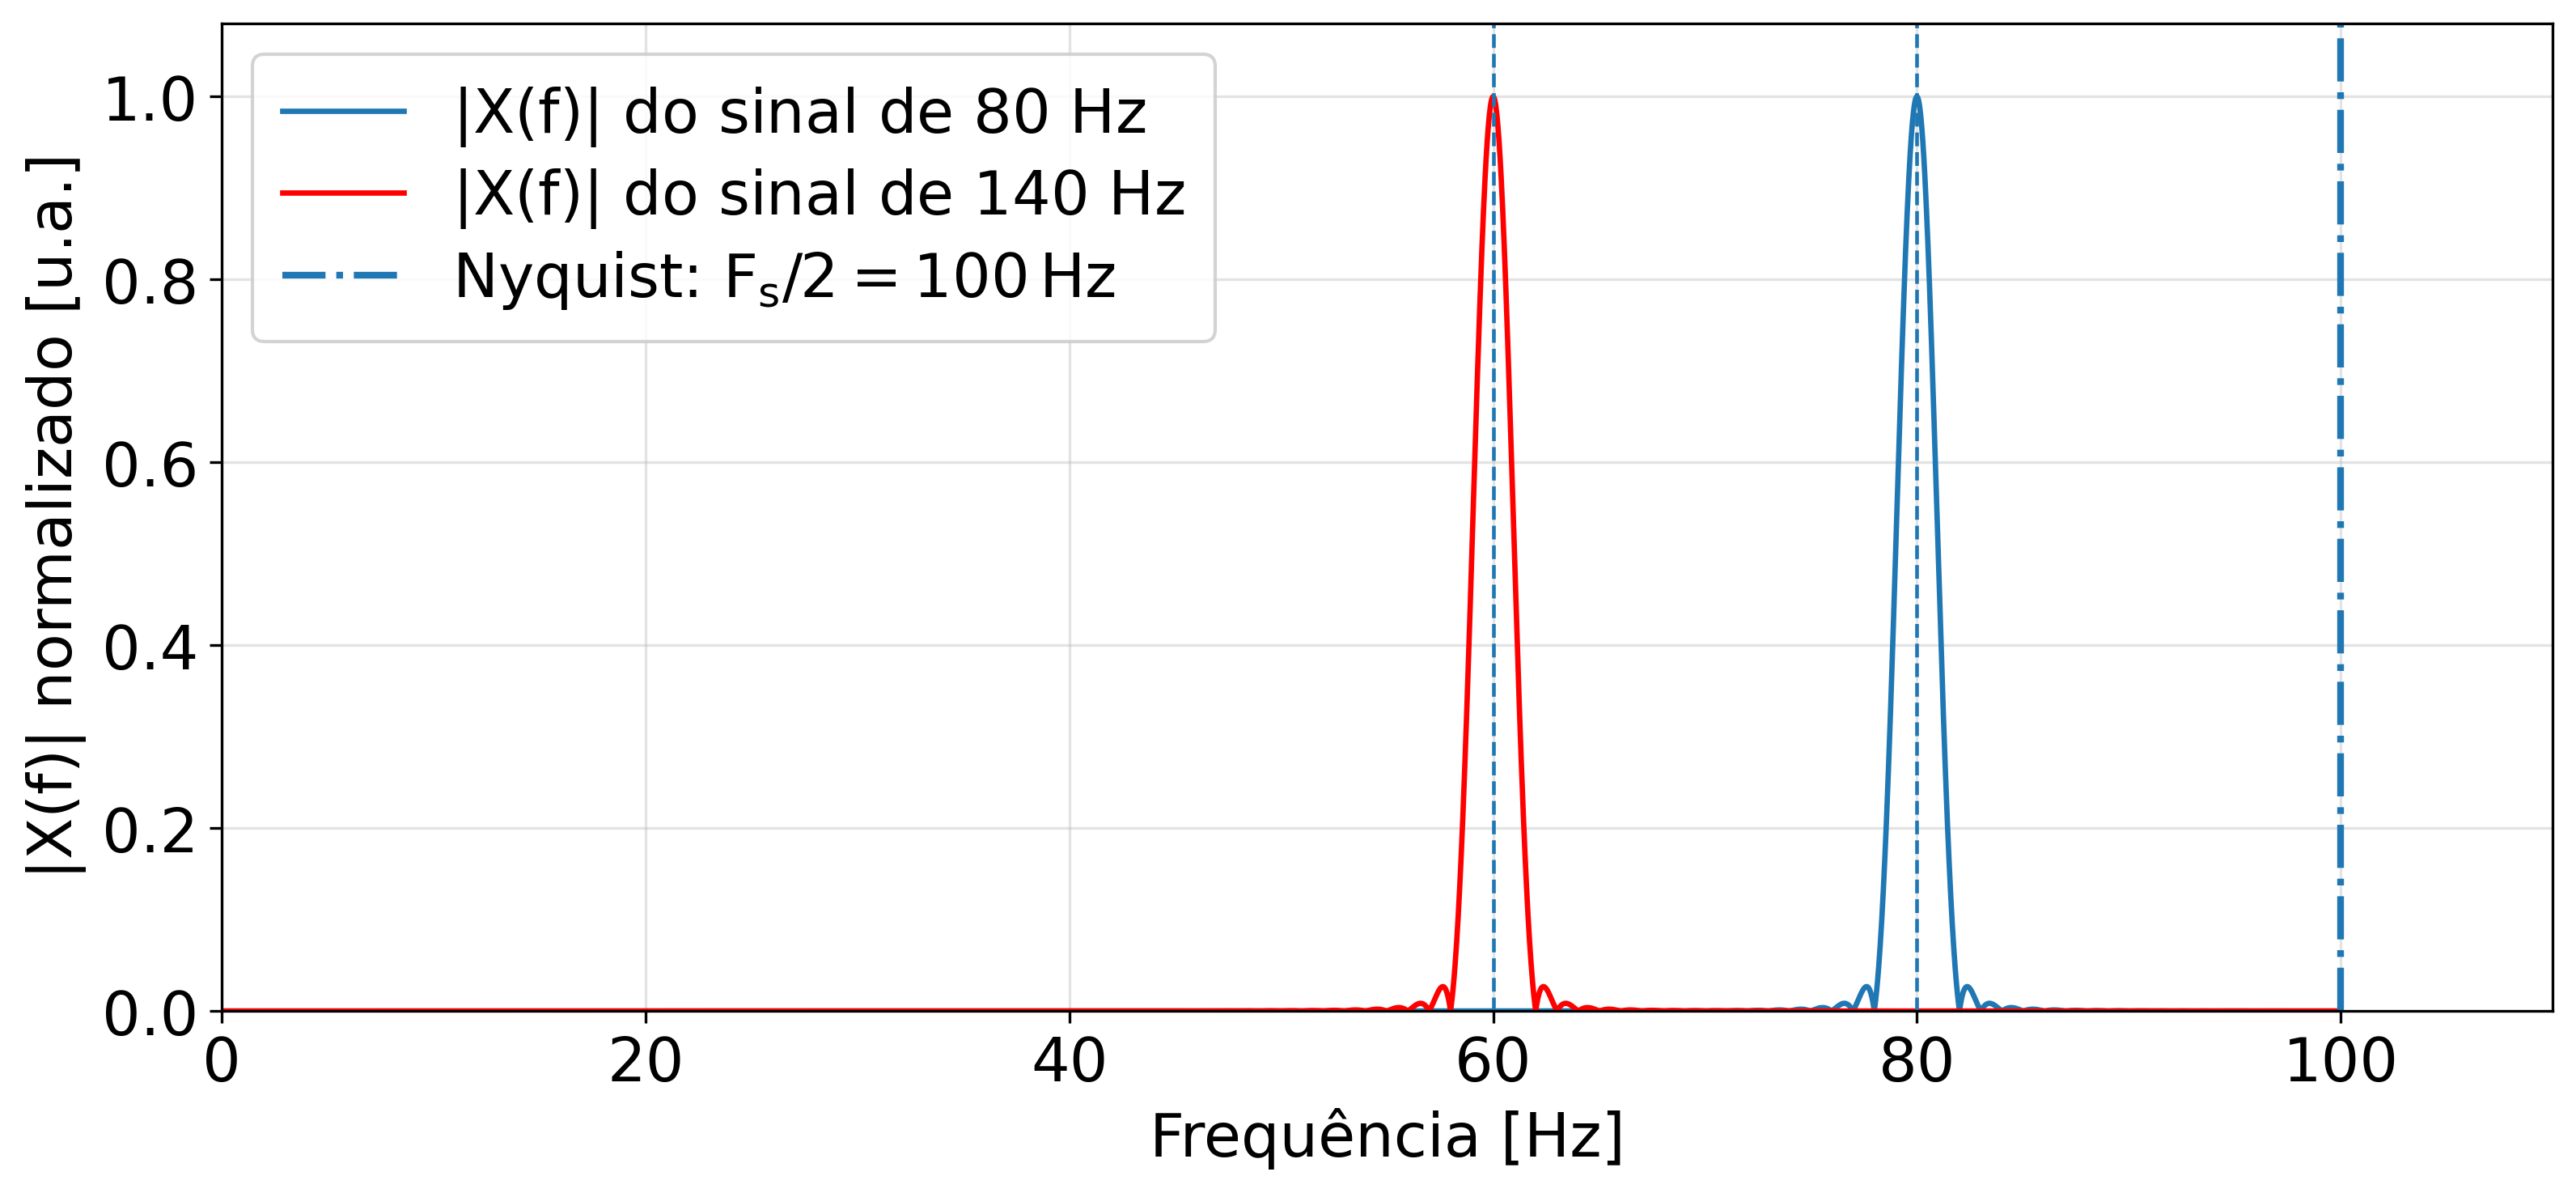
\includegraphics[width=\linewidth]{figuras/figura_dois_sinais.png}
    \caption[Aliasing na Transformada de Fourier de Sinais Amostrados]{Módulo normalizado da transformada de Fourier de dois sinais senoidais amostrados com frequência de amostragem $F_s=200$ Hz. O sinal original de 80 Hz é representado corretamente, pois sua frequência é inferior à frequência de Nyquist, dada por $F_s/2=100$ Hz. Por outro lado, o sinal original de 140 Hz excede o limite de Nyquist e sofre aliasing, aparecendo no espectro como um componente mascarado em 60 Hz, uma vez que $f_a=|140-200|=60$ Hz. As linhas tracejadas indicam as frequências observadas no espectro, enquanto a linha com traços e pontos representa a frequência de Nyquist.}
    \label{fig:aliasing}
\end{figure}

A definição da taxa de amostragem, portanto, não depende apenas de uma regra matemática geral, mas também das características fisiológicas do sinal, do tipo de análise pretendida e da arquitetura de aquisição adotada. Em uma plataforma modular como a desenvolvida neste trabalho, esse cuidado é ainda mais importante, pois diferentes módulos podem operar com sinais de naturezas bastante distintas, exigindo parâmetros de amostragem compatíveis com cada caso.

\subsection{Quantização, resolução e ruído de quantização}

Após a discretização temporal realizada pela amostragem, o sinal analógico também precisa ser discretizado em amplitude. Esse processo, denominado quantização, consiste em mapear o valor de cada amostra para o nível digital representável mais próximo. Esse mapeamento introduz uma diferença entre o valor analógico real da amostra e o valor digital selecionado, denominada erro de quantização. Em um conversor ideal, esse erro permanece limitado a aproximadamente metade do menor incremento representável pelo sistema, isto é, $\pm 1/2$ LSB~\cite{kester2008mt001}.

Considerando um conversor de $N$ bits e uma faixa de entrada de escala cheia $V_{FS}$, o tamanho de cada nível de quantização pode ser aproximado por

\begin{equation}
    \Delta = \frac{V_{FS}}{2^N},
\end{equation}

\noindent em que $\Delta$ representa a largura de um passo de quantização. Quanto maior o número de bits do conversor, menor é o valor de $\Delta$ e, consequentemente, maior é a capacidade do sistema de representar variações sutis do sinal analógico. Esse aspecto é particularmente relevante em sinais fisiológicos, pois muitos deles apresentam amplitudes reduzidas e podem ser degradados quando a resolução do sistema de aquisição é insuficiente.

Quando o erro de quantização é modelado como uma variável aleatória uniformemente distribuída entre $-\Delta/2$ e $+\Delta/2$, seu valor eficaz pode ser aproximado por

\begin{equation}
    e_{q,rms} = \frac{\Delta}{\sqrt{12}}.
\end{equation}

\noindent Essa aproximação permite relacionar a resolução do conversor à relação sinal-ruído teórica associada ao processo de quantização. Para um conversor ideal de $N$ bits e uma senoide de escala cheia, essa relação pode ser expressa por

\begin{equation}
    SNR \approx 6,02N + 1,76 \ \text{dB}.
\end{equation}

\noindent Assim, cada bit adicional na resolução do conversor aumenta a relação sinal-ruído teórica em cerca de 6 dB~\cite{kester2008mt001}. Essa relação, entretanto, representa uma condição ideal. Em sistemas reais, a qualidade da aquisição também é influenciada por ruído térmico, ruído da referência de tensão, não linearidades do conversor, interferências eletromagnéticas, ruído dos circuitos de condicionamento, artefatos de movimento e acoplamento da rede elétrica.

Em sinais fisiológicos, a relação entre a amplitude do sinal e a faixa de entrada do conversor é tão importante quanto a resolução nominal. Caso um sinal de baixa amplitude utilize apenas uma pequena parcela da faixa dinâmica disponível, parte da resolução efetiva do conversor deixa de ser aproveitada. Por isso, circuitos de condicionamento, amplificação e ajuste de faixa são frequentemente necessários antes da conversão analógico-digital, especialmente em sinais como ECG, PPG e outros sinais de baixa amplitude~\cite{charlton2022wearable_ppg,raus2025ecg_testing}.

Além da resolução nominal, deve-se considerar a resolução efetiva do sistema. Conversores de alta resolução podem apresentar número efetivo de bits inferior ao valor nominal em função de ruídos internos, taxa de amostragem selecionada, ganho programável, arquitetura de conversão e condições de operação. Por essa razão, parâmetros como número efetivo de bits, ruído referido à entrada e resolução livre de ruído são relevantes na avaliação prática de conversores analógico-digitais utilizados em sistemas de aquisição fisiológica~\cite{kester2008mt001}.

No contexto deste trabalho, esses conceitos justificam a escolha de um conversor de alta resolução e reforçam a necessidade de verificação experimental da cadeia de aquisição. A fidelidade final dos sinais adquiridos não depende apenas do número de bits especificado pelo fabricante, mas do comportamento integrado dos sensores, do condicionamento analógico, da conversão, da comunicação, do armazenamento e do processamento dos dados.

\subsection{Taxa de amostragem e conteúdo espectral}

A escolha da taxa de amostragem deve ser feita a partir do conteúdo espectral do sinal e do tipo de análise que se pretende realizar. Embora o critério de Nyquist-Shannon estabeleça uma condição mínima para evitar aliasing em sinais limitados em banda, a taxa de amostragem adotada em um sistema real normalmente deve considerar margens adicionais, limitações dos filtros anti-aliasing, resolução temporal desejada e preservação da morfologia do sinal~\cite{kester2008mt002}. Dessa forma, a escolha de $F_s$ não é apenas uma exigência matemática, mas uma decisão de projeto associada à qualidade da aquisição.

Sinais fisiológicos distintos apresentam conteúdos espectrais bastante diferentes. O ECG, por exemplo, concentra parcela relevante de sua energia em baixas frequências, mas a preservação adequada de componentes associados ao complexo QRS e à morfologia das ondas pode exigir taxas de amostragem superiores ao mínimo teórico~\cite{chu2023ecgsystem,su2023ecg_acquisition}. Em aplicações de monitoramento, taxas entre 250 Hz e 500 Hz são frequentemente utilizadas, enquanto aplicações que exigem maior detalhamento morfológico podem empregar taxas da ordem de 1 kHz~\cite{raus2025ecg_testing}. Assim, mesmo quando o conteúdo clínico principal se encontra em uma faixa relativamente baixa, a taxa de amostragem deve ser escolhida de modo a preservar as características temporais relevantes do sinal.

No caso do PPG, o sinal apresenta variações mais lentas quando comparado ao ECG, pois está associado às alterações de volume sanguíneo periférico durante o ciclo cardíaco. Ainda assim, a escolha da taxa de amostragem influencia a estimativa de frequência de pulso, variabilidade, forma de onda e parâmetros derivados~\cite{charlton2022wearable_ppg}. Estudos sobre variabilidade derivada de PPG indicam que a frequência mínima de amostragem deve ser avaliada conforme o parâmetro analisado e o erro tolerado, pois taxas muito baixas podem prejudicar a localização precisa dos pulsos e a análise temporal do sinal~\cite{beres2021ppg_sampling}.

A relação entre taxa de amostragem e conteúdo espectral também afeta a representação de formas de onda não senoidais. Sinais com transições rápidas, bordas abruptas ou componentes harmônicas relevantes exigem maior largura de banda para que sua morfologia seja preservada. Uma onda quadrada, por exemplo, pode ter frequência fundamental relativamente baixa, mas sua representação adequada depende da preservação de harmônicas ímpares de maior frequência. Quando essas componentes não são amostradas ou são atenuadas pelo sistema, a forma de onda digitalizada passa a apresentar bordas suavizadas e perda de detalhes temporais~\cite{kester2008mt002}.

Em arquiteturas multicanais, a taxa de amostragem deve ser analisada também em função da forma de aquisição dos canais. Quando um conversor analógico-digital multiplexado é utilizado para adquirir diferentes entradas de forma sequencial, a taxa máxima de conversão disponível precisa ser distribuída entre os canais ativos. Assim, a taxa efetiva por canal depende da taxa global de aquisição, do número de canais, do tempo de chaveamento, do tempo de estabilização do sinal e da rotina de comunicação com o microcontrolador. O assentamento após a comutação também pode depender da impedância de saída do circuito de condicionamento e das características da entrada do conversor. Esse aspecto é relevante para a proposta deste trabalho, pois a inclusão de novos sinais não deve comprometer a taxa mínima necessária para os canais já existentes~\cite{devi2020realtimedaq}.

Outro fator associado à taxa de amostragem é o volume de dados produzido. Desconsiderando o overhead do protocolo, a taxa bruta de dados pode ser estimada por

\begin{equation}
    R_d = N_c F_s N_b,
\end{equation}

\noindent em que $R_d$ é a taxa de dados, $N_c$ é o número de canais, $F_s$ é a taxa de amostragem por canal e $N_b$ é o número de bits transmitidos por amostra. Na implementação prática, devem ser acrescentados os campos de identificação, sequência, marcação temporal e verificação de integridade utilizados pelo protocolo. O aumento de $F_s$ melhora a resolução temporal e pode facilitar análises espectrais e morfológicas, mas também eleva a quantidade de dados transmitidos, armazenados e processados. Em sistemas portáteis e embarcados, essa decisão impacta a largura de banda da comunicação, o tamanho dos arquivos gerados, o consumo de memória, o processamento em tempo próximo ao real e o consumo de energia. Portanto, a taxa de amostragem deve ser definida como compromisso entre fidelidade do sinal, requisitos de análise, limitações da arquitetura e custo computacional da aquisição.

No contexto deste trabalho, a definição das taxas de amostragem deve considerar simultaneamente o conteúdo espectral de cada sinal fisiológico, a resolução desejada, a capacidade do conversor analógico-digital, a organização multicanal da aquisição e a necessidade de visualização em tempo próximo ao real. Essa abordagem permite que a plataforma seja configurada de forma compatível com diferentes módulos de aquisição, preservando a integridade temporal dos sinais e mantendo margem para expansão da arquitetura.


\section{Introdução à aquisição de sinais fisiológicos}

A aquisição de sinais fisiológicos constitui a base de sistemas de monitoramento biomédico, pois permite converter fenômenos associados ao funcionamento do corpo humano em informações observáveis, registráveis e passíveis de processamento. Como esses sinais podem ter naturezas elétricas, mecânicas, ópticas, térmicas ou químicas, sua aquisição exige cuidados específicos de instrumentação, condicionamento, amostragem, digitalização e filtragem. Em sistemas vestíveis e portáteis, esses elementos precisam ser considerados de forma integrada, uma vez que a qualidade final dos dados depende não apenas do sensor, mas de toda a cadeia de aquisição e processamento~\cite{ates2022wearable_sensors,vaghasiya2023wearable_telehealth}.

Nesta seção, são apresentados conceitos gerais relacionados aos sinais fisiológicos e à sua importância em aplicações de saúde, pesquisa e monitoramento. Em seguida, são discutidos os sinais de interesse para este trabalho, com ênfase em suas características fisiológicas, faixas típicas de frequência, requisitos de aquisição e principais desafios associados ao condicionamento e à digitalização.

\subsection{Definição e importância dos sinais fisiológicos na saúde e na pesquisa}

Sinais fisiológicos são manifestações elétricas, mecânicas, ópticas, térmicas ou químicas resultantes de processos biológicos do corpo humano. Esses sinais fornecem informações relevantes sobre o funcionamento de órgãos e sistemas, permitindo acompanhar respostas corporais a estímulos internos e externos. Em aplicações de monitoramento contínuo, sensores vestíveis e sistemas portáteis têm ampliado a possibilidade de registrar esses sinais fora de ambientes clínicos tradicionais, aproximando a aquisição das condições reais de rotina do usuário~\cite{ates2022wearable_sensors,vaghasiya2023wearable_telehealth}.

Na prática clínica, o monitoramento de parâmetros como frequência cardíaca, saturação periférica de oxigênio, temperatura corporal e ritmo respiratório contribui para observar alterações em relação a padrões esperados e acompanhar a evolução do estado fisiológico do paciente. Em pesquisa, esses sinais possibilitam o estudo de processos fisiológicos, o desenvolvimento de novas técnicas de aquisição, a validação de métodos de processamento e a construção de sistemas de apoio ao acompanhamento em saúde~\cite{huhn2022wearables_health_research,tan2024remote_patient_monitoring}.

Entretanto, a aquisição confiável desses sinais impõe desafios técnicos relevantes. Muitos sinais fisiológicos apresentam baixa amplitude, variações lentas, componentes transitórias ou morfologia sensível a ruídos e interferências. Além disso, podem ser afetados por artefatos de movimento, acoplamento da rede elétrica, instabilidade de contato entre sensor e corpo, variações individuais e limitações dos circuitos de condicionamento. Por esse motivo, a qualidade da aquisição depende da integração adequada entre sensor, condicionamento analógico, conversão analógico-digital, filtragem, armazenamento e processamento dos dados~\cite{ates2022wearable_sensors,charlton2022wearable_ppg}.

\subsection{Sinais empregados na avaliação experimental}

Embora a arquitetura proposta seja concebida para aquisição de diferentes sinais fisiológicos, a avaliação experimental deste trabalho concentra-se inicialmente em sinais eletrocardiográficos (ECG) e fotopletismográficos (PPG). Essa delimitação permite avaliar a cadeia de aquisição com sinais reais, de relevância fisiológica reconhecida, sem restringir a plataforma exclusivamente a essas duas modalidades. Ambos os sinais são amplamente utilizados em aplicações cardiovasculares e de monitoramento contínuo, além de apresentarem requisitos distintos de condicionamento, amostragem, resolução e filtragem, o que os torna adequados para demonstrar a flexibilidade inicial da arquitetura~\cite{hughes2023wearable_cardiovascular,charlton2022wearable_ppg}.

\subsubsection{Eletrocardiograma (ECG)}

O eletrocardiograma (ECG) é um dos sinais fisiológicos mais utilizados na análise da atividade elétrica cardíaca. Ele é obtido por meio de eletrodos posicionados na superfície corporal, que captam variações de potencial associadas aos processos de despolarização e repolarização do coração. O traçado eletrocardiográfico apresenta ondas, segmentos e intervalos de interesse fisiológico e clínico, entre os quais se destacam a onda P, associada à despolarização atrial, o complexo QRS, relacionado à despolarização ventricular, e a onda T, associada à repolarização ventricular~\cite{ardeti2023ecg,das2014ecg}. Uma representação esquemática desses elementos é apresentada na Figura~\ref{fig:rep_ecg}.

\begin{figure}[!htb]
    \centering
    \includegraphics[width=\linewidth]{figuras/ilustracao_ecg_ciclo_single.png}
    \caption[Representação esquemática do ciclo eletrocardiográfico, com identificação dos principais elementos.]{Representação esquemática do ciclo eletrocardiográfico, com identificação das ondas P, Q, R, S e T, do complexo QRS e dos intervalos PR e QT, além dos segmentos PR e ST. A onda P representa a despolarização atrial, o complexo QRS a despolarização ventricular e a onda T a repolarização ventricular.}
    \label{fig:rep_ecg}
\end{figure}

A análise da morfologia, da duração e da amplitude dessas componentes permite observar alterações associadas a diferentes condições cardíacas, como arritmias, bloqueios de condução e sinais compatíveis com isquemia~\cite{ardeti2023ecg}. Em sistemas com mais de uma derivação, a comparação entre sinais obtidos em posições distintas permite avaliar diferenças temporais e morfológicas da atividade cardíaca, ampliando as possibilidades de análise. Por esse motivo, o ECG é empregado tanto em equipamentos clínicos quanto em sistemas de monitoramento ambulatorial, vestível e contínuo~\cite{hughes2023wearable_cardiovascular}.

Para que as características do ECG sejam preservadas durante a digitalização, a taxa de amostragem deve ser compatível com a faixa de frequência de interesse e com o nível de detalhamento pretendido. Em aplicações de monitoramento, são frequentemente utilizadas taxas entre 250 Hz e 500 Hz, enquanto aplicações que exigem maior preservação morfológica podem empregar taxas da ordem de 1 kHz~\cite{chu2023ecgsystem,su2023ecg_acquisition,raus2025ecg_testing}. Essa escolha deve considerar não apenas o conteúdo espectral do sinal, mas também os filtros empregados, a resolução temporal desejada e os requisitos de processamento posterior.

Do ponto de vista da instrumentação, a aquisição do ECG impõe requisitos específicos ao sistema. Como se trata de um sinal de baixa amplitude e suscetível a interferências externas, a etapa analógica deve apresentar elevada impedância de entrada, alta rejeição de modo comum, baixa contribuição de ruído e capacidade de operar na presença de offsets de eletrodo. Esses aspectos são avaliados em normas e procedimentos de teste aplicáveis a equipamentos eletrocardiográficos, incluindo verificações de impedância de entrada, ruído, exatidão de amplitude, resposta em frequência e rejeição de interferências~\cite{raus2025ecg_testing}. Além disso, técnicas de filtragem analógica e digital são empregadas para reduzir interferência da rede elétrica, artefatos de movimento, deriva de linha de base e ruídos de alta frequência, buscando preservar a morfologia do sinal nos trechos associados às ondas, segmentos e intervalos utilizados em sua análise~\cite{ardeti2023ecg,chu2023ecgsystem}.

No contexto deste trabalho, o ECG é utilizado como um dos sinais principais de avaliação da arquitetura por combinar relevância fisiológica, disponibilidade de módulos de condicionamento e requisitos de aquisição suficientemente rigorosos para analisar a cadeia de conversão, comunicação, armazenamento e visualização. A presença de componentes morfológicas bem definidas no traçado também facilita a comparação temporal e morfológica entre o sinal adquirido pela plataforma e sinais de referência ou formas esperadas.

\subsubsection{Fotopletismografia (PPG)}

A fotopletismografia (PPG) é uma técnica óptica não invasiva empregada para detectar variações de volume sanguíneo em tecidos periféricos. Seu princípio de funcionamento baseia-se na emissão de luz sobre o tecido biológico e na medição da intensidade luminosa transmitida ou refletida, a qual varia em função das mudanças pulsáteis associadas ao fluxo sanguíneo~\cite{allen2007ppg}. A escolha do comprimento de onda depende do local de medição e do parâmetro fisiológico analisado. Em oximetria de pulso, são tipicamente utilizados emissores nas faixas do vermelho e do infravermelho, enquanto outras aplicações vestíveis de PPG, especialmente no punho, também podem empregar luz verde~\cite{charlton2022wearable_ppg}.

Esse sinal é amplamente empregado em dispositivos vestíveis e sistemas de monitoramento contínuo, pois permite acompanhar fenômenos relacionados ao pulso arterial de forma simples, portátil e pouco invasiva~\cite{charlton2022wearable_ppg,huhn2022wearables_health_research}. A partir da PPG, é possível obter informações associadas à frequência cardíaca, à perfusão periférica e à variabilidade do pulso. Em conjunto com medições ópticas em diferentes comprimentos de onda e modelos de processamento apropriados, a PPG também viabiliza aplicações como a oximetria de pulso~\cite{charlton2022wearable_ppg}. Além disso, por poder ser adquirida em diferentes regiões do corpo, como dedo, punho ou outras áreas periféricas, a técnica apresenta interesse em aplicações portáteis e de uso contínuo.

Do ponto de vista da aquisição, a PPG impõe desafios diferentes daqueles observados no ECG. Por se tratar de um sinal óptico, sua qualidade depende do acoplamento entre emissor, tecido e fotodetector, podendo ser afetada por artefatos de movimento, variações de contato, interferência luminosa ambiente, baixa perfusão periférica e diferenças individuais relacionadas às propriedades ópticas da pele e dos tecidos~\cite{charlton2022wearable_ppg,ates2022wearable_sensors}. Por esse motivo, são comuns estratégias como controle da intensidade luminosa, sincronização entre emissão e leitura, multiplexação de LEDs, filtragem digital e remoção de deriva de linha de base.

Em termos de digitalização, a componente pulsátil da PPG concentra-se tipicamente em baixas frequências, associadas ao ciclo cardíaco. Ainda assim, a taxa de amostragem deve ser escolhida conforme o tipo de análise pretendida, uma vez que estimativas de frequência de pulso, variabilidade e parâmetros derivados dependem da localização temporal adequada dos pulsos~\cite{beres2021ppg_sampling}. Taxas muito baixas podem prejudicar a identificação precisa dos máximos, mínimos e intervalos entre pulsos, enquanto taxas mais altas aumentam o volume de dados e o custo computacional da aquisição. Assim, a escolha da taxa de amostragem da PPG deve considerar o compromisso entre fidelidade temporal, ruído, processamento em tempo próximo ao real e capacidade de armazenamento.

No contexto deste trabalho, a PPG é utilizada como segundo sinal de avaliação por complementar o ECG na análise cardiovascular e por apresentar natureza física distinta, baseada em aquisição óptica. Essa diferença permite avaliar a arquitetura proposta em condições de aquisição mais amplas, envolvendo não apenas sinais elétricos de baixa amplitude, mas também sinais ópticos sujeitos a interferências mecânicas e ambientais. Dessa forma, a utilização conjunta de ECG e PPG contribui para demonstrar a adequação inicial da plataforma como base modular para aquisição contínua de múltiplos sinais fisiológicos.

\subsection{Sinais fisiológicos considerados para expansão da arquitetura}

Embora a avaliação experimental deste trabalho se concentre em ECG e PPG, a arquitetura proposta foi concebida como uma base modular para aquisição de diferentes sinais fisiológicos. Por essa razão, esta seção apresenta outros sinais relevantes como referência para expansão futura da plataforma. Esses sinais não constituem, nesta etapa, objeto de avaliação experimental completa, mas são discutidos por influenciarem requisitos gerais de projeto, como faixa de frequência, amplitude, taxa de amostragem, condicionamento analógico, resolução do conversor A/D e organização multicanal da aquisição.

\subsubsection{\texorpdfstring{Oximetria de pulso ($\mathrm{SpO}_2$)}{Oximetria de pulso (SpO2)}}

A oximetria de pulso é uma técnica não invasiva utilizada para estimar a saturação periférica de oxigênio no sangue, usualmente representada por $\mathrm{SpO}_2$. Seu princípio de funcionamento baseia-se na diferença de absorção óptica entre a oxi-hemoglobina e a desoxi-hemoglobina quando iluminadas em diferentes comprimentos de onda, tipicamente nas faixas do vermelho e do infravermelho~\cite{chan2013pulseox}. A partir da razão entre as componentes pulsáteis extraídas nesses dois comprimentos de onda, torna-se possível estimar a saturação de oxigênio associada ao pulso arterial.

Do ponto de vista instrumental, a oximetria está diretamente relacionada à fotopletismografia, uma vez que depende da aquisição confiável do sinal óptico pulsátil~\cite{chan2013pulseox,charlton2022wearable_ppg}. Por esse motivo, fatores como artefatos de movimento, variações de contato, interferência luminosa ambiente e baixos níveis de perfusão periférica, que afetam a PPG, também influenciam a qualidade da estimativa de $\mathrm{SpO}_2$. Em aplicações de monitoramento contínuo, isso torna necessário empregar estratégias de sincronização entre emissores ópticos e fotodetector, além de técnicas de filtragem e compensação que reduzam a degradação do sinal.

A relevância da oximetria para sistemas portáteis de monitoramento fisiológico decorre de sua ampla utilização no acompanhamento do estado respiratório e circulatório do usuário. Por se tratar de uma medição óptica não invasiva, compatível com módulos ópticos integrados e frequentemente associada à aquisição de PPG, a estimativa de $\mathrm{SpO}_2$ torna-se uma possibilidade natural de expansão para a arquitetura proposta.

\subsubsection{Temperatura corporal}

A temperatura corporal é um parâmetro fisiológico amplamente utilizado no acompanhamento do estado geral do organismo, podendo fornecer indícios de alterações metabólicas, inflamatórias e infecciosas. Sua medição pode ser realizada em superfícies cutâneas ou em regiões internas do corpo, dependendo do método empregado e do grau de precisão desejado. Em sistemas portáteis e de monitoramento contínuo, a medição em superfície tende a ser a abordagem mais viável, embora esteja mais sujeita à influência do ambiente, do local de posicionamento do sensor e das condições de contato com a pele~\cite{boano2011temperature,vaghasiya2023wearable_telehealth}.

Entre os sensores mais utilizados para esse tipo de aquisição estão os termistores e os termopares. O termistor apresenta variação de resistência em função da temperatura, enquanto o termopar gera uma força eletromotriz relacionada à diferença de temperatura entre a junção de medição e a junção de referência, sendo necessária a compensação da junção fria para uma estimativa adequada. Também é possível realizar medições sem contato, a partir da radiação térmica emitida pelo corpo, embora esse tipo de abordagem imponha cuidados adicionais de calibração, emissividade e sensibilidade ao ambiente~\cite{boano2011temperature}. Em todos os casos, a escolha do sensor depende do compromisso entre simplicidade de integração, precisão, tempo de resposta, consumo de energia e adequação à aplicação.

Do ponto de vista da aquisição, a temperatura impõe exigências menos severas de largura de banda do que sinais como ECG, PPG ou sEMG, uma vez que sua variação ocorre de forma relativamente lenta. Ainda assim, aspectos como resolução, calibração, estabilidade do contato com a pele e posição anatômica da medição permanecem fundamentais para a obtenção de dados confiáveis. Como diferentes regiões do corpo apresentam temperaturas distintas, a interpretação do sinal deve levar em conta o local em que a medição é realizada, especialmente em aplicações vestíveis. Para a arquitetura proposta, a temperatura representa um módulo de expansão de baixa taxa de amostragem, útil para avaliar a flexibilidade da plataforma em lidar com sinais de dinâmica lenta.

\subsubsection{Sinal respiratório}

O sinal respiratório corresponde às variações fisiológicas associadas ao ciclo de inspiração e expiração, podendo ser utilizado para acompanhar a frequência respiratória, a amplitude do movimento ventilatório e possíveis irregularidades no padrão de respiração~\cite{vitazkova2024resp}. Por se tratar de um parâmetro diretamente relacionado à função pulmonar e ao estado geral do organismo, sua observação contínua pode contribuir para o acompanhamento de diferentes condições clínicas e para a identificação de alterações respiratórias ao longo do tempo.

A aquisição desse sinal pode ser realizada de forma direta ou indireta. Entre os métodos diretos, destacam-se sensores de fluxo ou de pressão acoplados a máscaras, cânulas ou outros dispositivos específicos de medição respiratória. Já nos métodos indiretos, são frequentemente utilizadas bandas torácicas, sensores de deformação ou outros transdutores capazes de acompanhar a expansão e a contração do tórax ao longo do ciclo respiratório~\cite{vitazkova2024resp}. Em sistemas portáteis e vestíveis, abordagens indiretas tendem a ser mais compatíveis com a proposta de monitoramento contínuo, por oferecerem menor invasividade e maior conforto de uso.

Do ponto de vista da aquisição, o sinal respiratório apresenta componente predominante em baixas frequências, tipicamente inferior àquelas observadas em sinais cardíacos ou musculares. Essa característica reduz a exigência de largura de banda, mas não elimina os desafios de aquisição. A confiabilidade do sinal depende de estabilidade mecânica, posicionamento adequado do sensor e capacidade de distinguir o movimento respiratório de outras perturbações, como deslocamentos corporais e artefatos de movimento~\cite{vitazkova2024resp}. Assim, para a arquitetura proposta, o sinal respiratório representa uma possibilidade de expansão associada a baixas taxas de amostragem, mas com requisitos importantes de fixação, estabilidade e filtragem.

\subsubsection{Eletromiografia de superfície (sEMG)}

A eletromiografia de superfície, usualmente abreviada como sEMG, é uma modalidade não invasiva de eletromiografia (EMG) utilizada para registrar a atividade elétrica associada à contração muscular por meio de eletrodos posicionados sobre a pele. O sinal resulta da soma dos potenciais de ação das unidades motoras ativas na região de captação e pode fornecer informações sobre ativação muscular, esforço, fadiga, coordenação motora e resposta a protocolos de reabilitação~\cite{al_ayyad2023emg_rehabilitation,cheng2023flexible_semg}.

Em aplicações de monitoramento fisiológico, a sEMG pode ser útil em contextos como reabilitação, análise funcional, treinamento físico, controle de próteses e interfaces homem-máquina. Entretanto, sua aquisição impõe requisitos mais exigentes do que sinais de dinâmica lenta, como temperatura ou respiração. O conteúdo espectral da EMG de superfície ocupa uma faixa de frequência mais ampla, exigindo taxas de amostragem superiores às utilizadas em sinais como PPG e respiração. Além disso, a interpretação do sinal depende fortemente do posicionamento dos eletrodos, da distância intereletrodo, da preparação da pele, do músculo avaliado e da presença de interferência de músculos vizinhos~\cite{al_ayyad2023emg_rehabilitation,cheng2023flexible_semg}.

Do ponto de vista instrumental, a sEMG requer uma cadeia de aquisição com boa rejeição de modo comum, baixo ruído, largura de banda adequada e filtragem capaz de reduzir interferência da rede elétrica, artefatos de movimento e componentes indesejadas de baixa frequência. Em análises mais avançadas, o uso de múltiplos canais pode ampliar a informação disponível, permitindo avaliar diferenças espaciais de ativação e, em algumas configurações, estimar parâmetros relacionados à propagação dos potenciais ao longo do músculo. Essa característica aumenta a utilidade do sinal, mas também eleva a demanda sobre a arquitetura de aquisição, pois exige maior taxa global de amostragem, organização multicanal e maior volume de dados transmitidos e armazenados.

No contexto deste trabalho, a sEMG é tratada como uma possibilidade de expansão futura da plataforma, e não como parte do ensaio experimental principal. Sua inclusão como referência é relevante porque representa um caso mais exigente para a arquitetura modular: além de demandar condicionamento analógico específico, pode requerer múltiplos canais, maior largura de banda e maior taxa de amostragem efetiva por canal. Assim, a análise da sEMG contribui para avaliar a escalabilidade do sistema e os limites práticos da proposta quando novos sinais fisiológicos forem incorporados.

\section{Requisitos de aquisição dos sinais}

Os sinais fisiológicos discutidos neste capítulo apresentam naturezas distintas e, por isso, impõem exigências diferentes ao sistema de aquisição. Parâmetros como faixa de frequência, amplitude, resolução necessária, sensibilidade a ruídos, forma de acoplamento ao corpo e condições de posicionamento variam conforme o tipo de sinal e a aplicação pretendida. Dessa forma, o desenvolvimento de uma plataforma modular de monitoramento fisiológico exige que essas diferenças sejam consideradas desde a etapa de projeto, tanto na escolha dos sensores e circuitos de condicionamento quanto na definição da taxa de amostragem, da resolução da aquisição e das estratégias de filtragem.

Com o objetivo de sintetizar essas exigências e orientar as escolhas técnicas adotadas neste trabalho, a Tabela~\ref{tab:req-sinais} apresenta valores típicos de referência para os sinais utilizados na avaliação experimental e para os sinais considerados como possibilidades de expansão da arquitetura. Esses valores não constituem limites absolutos nem esgotam todas as possibilidades de projeto, pois podem variar conforme o sensor, a aplicação, o método de aquisição e o nível de fidelidade desejado. Ainda assim, fornecem um panorama comparativo útil para compreender as demandas de cada sinal e justificar a organização modular proposta para o sistema.

\begin{landscape}
\footnotesize
\begin{longtable}{
  @{}
  >{\raggedright\arraybackslash}m{0.10\linewidth}
  >{\centering\arraybackslash}m{0.15\linewidth}
  >{\centering\arraybackslash}m{0.16\linewidth}
  >{\centering\arraybackslash}m{0.13\linewidth}
  >{\raggedright\arraybackslash}m{0.18\linewidth}
  >{\raggedright\arraybackslash}m{0.19\linewidth}
  @{}
}
    \caption{Requisitos típicos de aquisição para os sinais fisiológicos considerados na plataforma}
    \label{tab:req-sinais}\\

    \toprule
    \textbf{Sinal} &
    \textbf{Faixa de frequência típica} &
    \textbf{Taxa de amostragem típica} &
    \textbf{Resolução da aquisição} &
    \textbf{Faixa do sinal / condição} &
    \textbf{Observações} \\
    \midrule
    \endfirsthead

    \toprule
    \textbf{Sinal} &
    \textbf{Faixa de frequência típica} &
    \textbf{Taxa de amostragem típica} &
    \textbf{Resolução da aquisição} &
    \textbf{Faixa do sinal / condição} &
    \textbf{Observações} \\
    \midrule
    \endhead

    \multicolumn{6}{@{}l}{\textit{Sinais utilizados na avaliação experimental}}\\
    \midrule

    \textbf{ECG} &
    $0,05$--$150\,\text{Hz}$ &
    $250$--$1000\,\text{Hz}$ &
    $12$ bits ou superior, condicionado à faixa de entrada, ao ganho e ao ruído &
    Baixa amplitude, tipicamente na ordem de $\mu\text{V}$ a poucos $\text{mV}$ &
    Requer elevada impedância de entrada, rejeição de modo comum, mitigação de interferência de rede, redução de deriva de linha de base e preservação morfológica do traçado~\cite{ardeti2023ecg,chu2023ecgsystem,raus2025ecg_testing}. \\

    \textbf{PPG} &
    Predominantemente baixa frequência; componente pulsátil associada ao ciclo cardíaco &
    Tipicamente dezenas a centenas de Hz, conforme o parâmetro analisado &
    $12$ bits ou superior, condicionado ao sensor, à faixa dinâmica e ao ruído &
    Aquisição óptica por LED e fotodetector em modo transmissivo ou reflexivo &
    Sensível a movimento, pressão de contato, luz ambiente, baixa perfusão e propriedades ópticas da pele; exige filtragem e, em muitos casos, sincronização entre emissão luminosa e leitura~\cite{charlton2022wearable_ppg,beres2021ppg_sampling}. \\

    \midrule
    \multicolumn{6}{@{}l}{\textit{Sinais considerados para expansão da arquitetura}}\\
    \midrule

    \textbf{Oximetria de pulso} &
    Relacionada à componente pulsátil da PPG &
    Dependente do sensor e da alternância entre comprimentos de onda &
    Definida pelo módulo óptico ou pelo conversor utilizado &
    Estimativa de $\mathrm{SpO}_2$ a partir de medições em vermelho e infravermelho &
    Depende da qualidade dos sinais ópticos pulsáteis, da separação entre componentes AC/DC, da baixa interferência por movimento e da calibração do método de estimação~\cite{chan2013pulseox,charlton2022wearable_ppg}. \\

    \textbf{Temperatura corporal} &
    Variação lenta, próxima de DC &
    $1$--$10\,\text{Hz}$, conforme aplicação &
    Definida conforme sensor; resolução térmica típica de interesse em torno de $0,1\,^\circ\text{C}$ &
    Medição cutânea ou interna; em aplicações vestíveis, usualmente superfície da pele &
    Exige calibração, estabilidade de contato, consideração do local anatômico de medição e compensação de influência ambiental~\cite{boano2011temperature,vaghasiya2023wearable_telehealth}. \\

    \textbf{Respiração} &
    Baixa frequência, geralmente inferior à de sinais cardíacos e musculares &
    $10$--$100\,\text{Hz}$, conforme sensor e análise pretendida &
    Definida conforme sensor e arquitetura &
    Aquisição por sensores de fluxo, pressão, deformação ou bandas torácicas &
    Requer estabilidade mecânica, posicionamento adequado e separação entre movimento respiratório e artefatos corporais~\cite{vitazkova2024resp}. \\

    \textbf{sEMG} &
    Aproximadamente $10$--$500\,\text{Hz}$ em aplicações de superfície &
    $1000$--$2000\,\text{Hz}$ ou superior, conforme aplicação &
    $12$ bits ou superior, condicionado à faixa de entrada, ao ganho e ao ruído &
    Baixa amplitude, tipicamente na ordem de $\mu\text{V}$ a poucos $\text{mV}$ &
    Exige alto ganho, boa rejeição de modo comum, largura de banda adequada, filtragem de interferência de rede e cuidado com posicionamento dos eletrodos; múltiplos canais podem ser necessários para análises mais avançadas~\cite{al_ayyad2023emg_rehabilitation,cheng2023flexible_semg}. \\

    \bottomrule
\end{longtable}

\begin{flushleft}
    \footnotesize
    \textit{Notas:} Os valores apresentados são referências típicas de projeto e podem variar conforme o sensor, a aplicação, o método de aquisição e o nível de fidelidade desejado. As referências apresentadas na coluna de observações estão associadas aos parâmetros indicados na respectiva linha. A resolução nominal, isoladamente, não determina o desempenho da aquisição, que também depende da faixa de entrada, do ganho, do ruído referido à entrada e do número efetivo de bits. A tabela distingue os sinais utilizados na avaliação experimental, ECG e PPG, dos sinais considerados como possibilidades de expansão da arquitetura modular.
\end{flushleft}

\normalsize
\end{landscape}

\section{Condicionamento e filtragem de sinais fisiológicos}

O condicionamento de sinais fisiológicos corresponde ao conjunto de etapas responsáveis por adaptar o sinal captado pelo sensor às condições necessárias para sua digitalização e processamento. Essa etapa pode envolver amplificação, limitação de banda, remoção de offset, rejeição de interferências, ajuste de faixa dinâmica, proteção das entradas do circuito e filtragem analógica. Em sinais de baixa amplitude, como ECG e sEMG, o condicionamento é especialmente relevante, pois pequenas interferências provenientes da rede elétrica, do movimento do usuário ou do acoplamento entre sensor e corpo podem comprometer a morfologia do sinal adquirido~\cite{ardeti2023ecg,raus2025ecg_testing}.

A filtragem, nesse contexto, não deve ser compreendida apenas como uma etapa de remoção de ruído, mas como parte do compromisso entre fidelidade do sinal, estabilidade da aquisição e preservação das componentes fisiológicas de interesse. Dependendo da arquitetura adotada, parte do tratamento pode ser realizada antes da conversão analógico-digital, por meio de circuitos analógicos, enquanto etapas adicionais podem ser implementadas digitalmente no microcontrolador ou no sistema computacional responsável pela visualização, armazenamento e processamento dos dados~\cite{chu2023ecgsystem,ardeti2023ecg}.

\subsection{Condicionamento e filtragem analógica}

Os filtros analógicos são empregados antes da digitalização com o objetivo de limitar a banda de entrada do conversor, reduzir interferências e evitar que componentes indesejadas sejam incorporadas ao sinal digitalizado. Uma função importante dessa etapa é a filtragem anti-aliasing, que atenua componentes acima da frequência de Nyquist antes da conversão A/D, reduzindo a possibilidade de que frequências superiores à banda de interesse sejam rebatidas para faixas mais baixas do espectro~\cite{kester2008mt002}. Assim, a filtragem analógica está diretamente relacionada à escolha da taxa de amostragem e à preservação do conteúdo espectral útil do sinal.

Em sinais fisiológicos, é comum empregar combinações de filtros passa-alta, passa-baixa e rejeita-faixa, escolhidos conforme o conteúdo espectral do sinal e as principais fontes de interferência presentes no sistema. Filtros passa-alta podem ser utilizados para reduzir deriva de linha de base, offsets lentos e variações associadas ao movimento ou ao contato imperfeito do sensor. Filtros passa-baixa, por sua vez, atenuam componentes de alta frequência que não pertencem à banda útil do sinal e contribuem para a limitação da banda antes da amostragem~\cite{chu2023ecgsystem,ardeti2023ecg}.

A interferência da rede elétrica, normalmente em 50 Hz ou 60 Hz, é uma fonte recorrente de ruído em sinais fisiológicos, especialmente em sinais bioelétricos adquiridos por eletrodos. Uma estratégia comum para atenuá-la é o uso de filtros rejeita-faixa, também chamados de filtros \textit{notch}. Entretanto, a aplicação desse tipo de filtro deve ser feita com cautela, pois a remoção de uma faixa estreita do espectro pode interferir em componentes úteis do sinal, dependendo da aplicação e da banda de interesse. No ECG, por exemplo, a redução da interferência de rede deve ser equilibrada com a preservação da morfologia das ondas, segmentos e intervalos utilizados na análise do traçado~\cite{ardeti2023ecg,raus2025ecg_testing}.

Além da filtragem, a etapa analógica também pode envolver amplificação e ajuste de faixa dinâmica. Como muitos sinais fisiológicos apresentam amplitudes reduzidas, é necessário adequar o nível do sinal à faixa de entrada do conversor A/D, evitando tanto a saturação quanto o uso de uma parcela muito pequena da faixa disponível. Esse ajuste é importante porque a resolução efetiva da aquisição depende não apenas do número de bits do conversor, mas também da relação entre a amplitude do sinal e a faixa de entrada utilizada~\cite{kester2008mt001}. Dessa forma, o condicionamento analógico contribui diretamente para a qualidade final da digitalização.

\subsection{Filtragem digital}

Após a conversão A/D, a filtragem digital amplia a capacidade de tratamento do sinal, permitindo maior flexibilidade no ajuste da resposta em frequência e na implementação de diferentes estratégias de processamento. Em arquiteturas embarcadas e modulares, como a adotada neste trabalho, essa etapa pode ser distribuída entre o microcontrolador e o sistema computacional responsável pela recepção, visualização e armazenamento dos dados. A definição do local de processamento depende da latência aceitável, do custo computacional, da taxa de amostragem, do número de canais e da necessidade de preservar dados brutos para análise posterior.

Entre as abordagens mais utilizadas estão os filtros IIR e FIR. Filtros IIR, do inglês \textit{Infinite Impulse Response}, geralmente exigem menor número de coeficientes para alcançar determinada resposta em frequência, o que os torna atrativos em sistemas com recursos computacionais limitados. Dependendo do projeto, esses filtros podem apresentar resposta de fase não linear, o que deve ser considerado quando a morfologia temporal do sinal é relevante. Filtros FIR, do inglês \textit{Finite Impulse Response}, podem ser projetados com fase linear, característica útil quando se deseja preservar relações temporais entre componentes do sinal, embora normalmente demandem maior ordem e maior custo de processamento.

A escolha entre filtros IIR e FIR depende do compromisso entre complexidade computacional, resposta em fase, estabilidade numérica e fidelidade do sinal processado. Em sinais fisiológicos, essa decisão deve considerar não apenas a atenuação desejada fora da banda útil, mas também o impacto da filtragem sobre parâmetros extraídos posteriormente, como intervalos temporais, amplitude de picos, morfologia de ondas e componentes espectrais. Em sinais como ECG e PPG, alterações excessivas na forma de onda podem comprometer análises baseadas em detecção de picos, intervalos e variabilidade~\cite{ardeti2023ecg,charlton2022wearable_ppg}.

No contexto deste trabalho, a filtragem digital é considerada uma etapa complementar ao condicionamento analógico. A arquitetura deve permitir tanto a visualização de sinais tratados para acompanhamento durante a aquisição quanto a preservação dos dados brutos para reprocessamento posterior. Essa separação é importante porque filtros aplicados durante a aquisição podem auxiliar na operação do sistema, mas a disponibilidade dos dados originais, acompanhados da versão do software e dos parâmetros de processamento, permite avaliar diferentes métodos, ajustar configurações e comparar resultados de forma reprodutível.



% ==============================================================================
% Metodologia
% ==============================================================================
\chapter{Materiais e Métodos}
\label{chap:MM}

\section{Visão geral dos Métodos Propostos}
\label{sec:visao_geral_metodologia}

Este capítulo apresenta os materiais utilizados, a arquitetura implementada, os blocos de hardware e software desenvolvidos e os procedimentos adotados para aquisição e validação dos sinais tratados neste trabalho. A plataforma foi organizada como um sistema modular de aquisição contínua, no qual módulos específicos de captação e condicionamento são conectados a um núcleo comum de digitalização, controle, processamento e visualização.

O desenvolvimento metodológico foi dividido em quatro etapas principais. A primeira correspondeu à definição e à integração da arquitetura de hardware. A segunda compreendeu a implementação do firmware responsável pelo controle do ADS1256, pela organização das amostras e pela transmissão dos dados. A terceira envolveu o desenvolvimento do programa de aquisição e visualização executado na Raspberry Pi. Por fim, a quarta etapa correspondeu à realização dos ensaios experimentais e à análise dos sinais obtidos.

A avaliação da plataforma foi organizada em duas frentes complementares. Na primeira, foram utilizados sinais conhecidos gerados em bancada. Esses sinais foram adquiridos simultaneamente pela plataforma desenvolvida e por um osciloscópio utilizado como instrumento de referência, permitindo comparar suas representações no domínio do tempo e da frequência. Na segunda frente, foram realizadas aquisições de ECG e PPG, com o objetivo de avaliar a capacidade funcional do sistema de registrar sinais fisiológicos, observar suas características morfológicas e identificar ruídos e artefatos presentes nas medições. Essa segunda etapa possui caráter instrumental e funcional, não constituindo validação clínica ou diagnóstica.


\section{Arquitetura geral do sistema}
\label{sec:arquitetura_geral}

A arquitetura geral do sistema é apresentada na Figura~\ref{fig:arquitetura}. A plataforma foi organizada em blocos funcionais distribuídos ao longo de uma cadeia de captação, condicionamento, conversão analógico-digital, controle, processamento e visualização. Inicialmente, os sinais fisiológicos são captados por módulos específicos, responsáveis por fornecer saídas analógicas compatíveis com a etapa de digitalização. Em seguida, esses sinais são encaminhados ao ADS1256, que realiza a conversão das tensões analógicas em valores quantizados.

\begin{figure}[!htb]
    \centering
    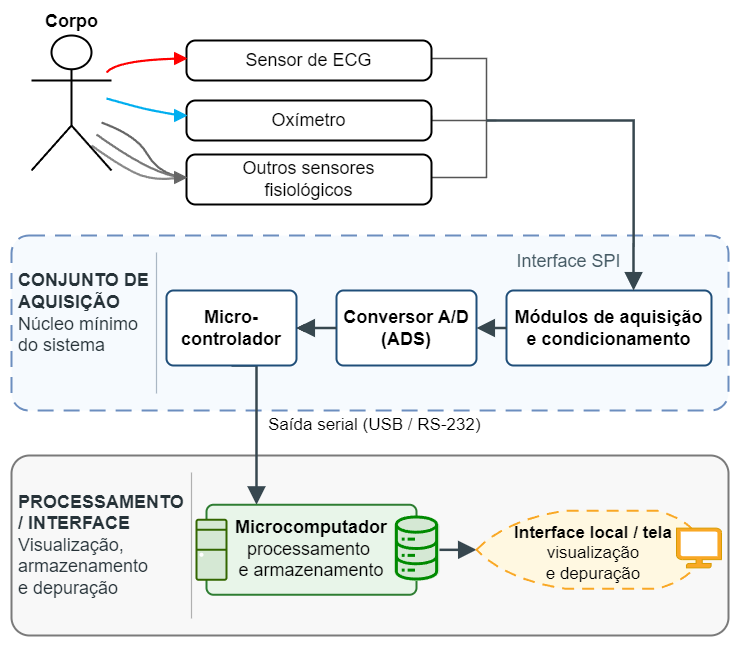
\includegraphics[width=\linewidth]{figuras/arquitetura_sistema.png}
    \caption[Arquitetura funcional da plataforma de aquisição de sinais fisiológicos]{Arquitetura funcional da plataforma de aquisição de sinais fisiológicos. Os sinais analógicos são digitalizados pelo ADS1256, enquanto a STM32 Black Pill controla a seleção dos canais, organiza as amostras e realiza sua transmissão serial. Na Raspberry Pi 3, os dados são separados, processados, visualizados nos domínios do tempo e da frequência e armazenados. A interação local com o sistema é feita por uma tela sensível ao toque.}
    \label{fig:arquitetura}
\end{figure}

A leitura do conversor é gerenciada por uma placa STM32 Black Pill. O microcontrolador controla a seleção das entradas do ADS1256, recebe as amostras digitalizadas, identifica o canal correspondente e organiza os dados para transmissão.

Os dados são encaminhados por comunicação serial à Raspberry Pi 3, na qual é executado o programa principal da plataforma. Essa etapa é responsável pela recepção e separação dos canais, aplicação dos procedimentos de processamento digital, visualização dos sinais no domínio do tempo, cálculo de sua representação espectral e armazenamento das aquisições. A Raspberry Pi também é conectada a uma tela sensível ao toque, utilizada para interação local com o sistema.

A distribuição das tarefas separa as operações sensíveis à temporização das operações de processamento e interface. A STM32 permanece responsável pelo controle do conversor e pelo transporte das amostras, enquanto a Raspberry Pi executa as tarefas de maior nível, como visualização, filtragem e armazenamento. Dessa forma, alterações na interface gráfica não exigem modificações na cadeia analógica de aquisição.

\section{Especificações e escolhas dos materiais}
\label{sec:materiais_hardware}

Esta seção apresenta os componentes de hardware utilizados na implementação do sistema, organizados conforme sua função na cadeia de aquisição. Inicialmente, são descritos os módulos responsáveis pela captação e pelo condicionamento dos sinais fisiológicos. Em seguida, são apresentados o conversor analógico-digital, o microcontrolador responsável pelo controle da aquisição, o microcomputador utilizado no processamento e na interface local e os instrumentos de bancada empregados nos ensaios experimentais.

As especificações apresentadas nesta seção correspondem às características relevantes dos componentes selecionados. Os parâmetros efetivamente configurados, as conexões elétricas e a distribuição dos canais são apresentados posteriormente, na Seção~\ref{sec:integracao_hardware}.

\subsection{Módulos de aquisição dos sinais}
\label{subsec:modulos_aquisicao}

A camada de entrada do sistema é formada por módulos específicos de aquisição, responsáveis por converter os fenômenos fisiológicos de interesse em sinais elétricos adequados à etapa de digitalização. A utilização de módulos distintos decorre das diferenças entre ECG e PPG quanto ao princípio físico de medição, à amplitude dos sinais, ao conteúdo espectral e aos requisitos de condicionamento. Neste trabalho, foram utilizados dois módulos para aquisição de ECG e um módulo para aquisição de PPG para a validação da arquitetura.

Para a aquisição dos dois canais de ECG, foram empregados dois módulos baseados no circuito integrado AD8232, cada um associado a um canal independente. O AD8232 é um circuito de condicionamento destinado à aquisição de ECG e de outros biopotenciais, integrando um amplificador de instrumentação, recursos configuráveis de filtragem, circuito de acionamento do eletrodo de referência e mecanismos de detecção de desconexão dos eletrodos~\cite{analogdevices_ad8232}.

O estágio de amplificação de instrumentação do AD8232 apresenta ganho interno igual a 100, rejeição de modo comum mínima de 80~dB entre corrente contínua e 60~Hz e impedância de entrada diferencial da ordem de gigaohms. O circuito integrado opera com alimentação entre 2,0~V e 3,5~V e possui consumo típico de 170~$\mu$A~\cite{analogdevices_ad8232}. Essas características são adequadas à aquisição de sinais de baixa amplitude captados por eletrodos superficiais.

A aquisição de PPG foi realizada com o Pulse Sensor Amped, desenvolvido pela World Famous Electronics. O módulo utiliza um emissor de luz verde e o sensor de luz ambiente APDS-9008 para detectar as variações de intensidade luminosa refletida pelo tecido periférico durante a propagação da onda de pulso~\cite{worldfamous_pulsesensor_amped}. A placa incorpora um circuito ativo de filtragem e amplificação, fornecendo em sua saída uma tensão analógica que varia de acordo com as alterações relativas da luz refletida.

O Pulse Sensor Amped admite alimentação entre 3~V e 5~V e apresenta consumo aproximado de 4~mA quando alimentado em 5~V. O circuito posiciona o sinal de saída em torno de metade da tensão de alimentação sobre o qual se manifesta a componente pulsátil do fotopletismograma~\cite{worldfamous_pulsesensor_amped}. A saída analógica do sensor é encaminhada ao ADS1256 para digitalização.

\subsection{Conversor A/D ADS1256}
\label{subsec:ads1256}

A digitalização dos sinais analógicos é realizada pelo ADS1256, fabricado pela Texas Instruments. Trata-se de um conversor A/D delta-sigma de quarta ordem, com resolução nominal de 24 bits, multiplexador de entradas, amplificador de ganho programável e filtro digital configurável~\cite{ti_ads1256}. A comunicação com o dispositivo é realizada por uma interface serial compatível com SPI.

O ADS1256 dispõe de oito entradas analógicas, que podem ser utilizadas como oito entradas referenciadas a um terminal comum ou organizadas como até quatro entradas diferenciais. Neste trabalho, foi selecionado o modo diferencial, no qual cada amostra representa a diferença de potencial entre duas entradas do multiplexador. Essa configuração permite associar um par de entradas a cada sinal adquirido, reduzindo a influência de tensões presentes simultaneamente nos dois terminais, desde que sejam respeitados os limites de modo comum do conversor.

O conversor apresenta taxas de saída de dados programáveis de até 30~mil amostras por segundo e amplificador de ganho programável com valores de até 64. O fabricante especifica resolução livre de ruído de até 23 bits em determinadas condições de operação~\cite{ti_ads1256}.

A alimentação analógica do circuito integrado é de 5~V, enquanto a alimentação digital pode variar entre 1,8~V e 3,6~V. Sua interface serial é tolerante a sinais de 5~V. O ADS1256 também oferece procedimentos internos de calibração de ganho e deslocamento, além de um indicador de dado disponível, utilizado para sinalizar a conclusão de uma conversão~\cite{ti_ads1256}.

\subsection{Microcontrolador STM32 Black Pill}
\label{subsec:stm32_blackpill}

O controle da conversão e da transmissão dos dados é realizado por uma placa Black Pill baseada no microcontrolador STM32F411CEU6, da STMicroelectronics. O dispositivo possui núcleo Arm Cortex-M4 de 32 bits, unidade de ponto flutuante, frequência máxima de operação de 100~MHz, 512~kB de memória de programa e 128~kB de memória de dados~\cite{st_stm32_modelo}. Esses recursos permitem controlar a leitura multicanal do ADS1256, organizar as amostras adquiridas e realizar sua transmissão contínua para a unidade de processamento.

A comunicação entre a STM32 e o ADS1256 é realizada por meio da interface SPI. Por essa interface, o microcontrolador configura os registradores do conversor, seleciona os pares de entradas diferenciais, aguarda a disponibilização de novas amostras e recebe os valores quantizados de 24 bits. A comunicação com a Raspberry Pi 3 Model B+ é realizada por USB CDC.

Na arquitetura proposta, a STM32 é responsável por inicializar e configurar o ADS1256, controlar o chaveamento das entradas, realizar a leitura das amostras, identificar o canal de origem e organizar os dados antes de sua transmissão.

Para diagnóstico e monitoramento, foi conectada à STM32 uma tela TFT de 1,8~polegadas com comunicação SPI. Essa tela foi empregada como recurso auxiliar de depuração, permitindo apresentar mensagens, estados internos da aquisição e resultados preliminares dos testes diretamente no conjunto formado pela STM32 e pelo ADS1256.

Essa divisão mantém no microcontrolador as tarefas diretamente relacionadas à regularidade temporal da aquisição. O processamento digital dos sinais, a interface gráfica principal e o armazenamento permanente dos registros são executados na Raspberry Pi, evitando que operações de visualização interfiram diretamente na rotina de leitura do conversor.

\subsection{Raspberry Pi e interface local}
\label{subsec:raspberry_interface}

O processamento principal da plataforma é realizado por uma Raspberry Pi 3 Model B+. Esse microcomputador utiliza o sistema em chip Broadcom BCM2837B0, composto por um processador de quatro núcleos e arquitetura de 64 bits, com frequência de operação de 1,4~GHz, e dispõe de 1~GB de memória~\cite{raspberrypi3_modelo}. Essas características permitem executar o sistema operacional, o programa de aquisição, os procedimentos de processamento digital e a interface gráfica local em uma mesma plataforma embarcada.

O sistema operacional utilizado é a distribuição Raspberry Pi OS Lite 32-bit, instalada em um cartão microSD com capacidade de 64~GB. O cartão é empregado tanto para armazenamento do sistema e do programa quanto para registro dos arquivos produzidos durante as aquisições.

A Raspberry Pi recebe os dados enviados pela STM32 pelo canal USB CDC. Após a recepção, o programa executado no microcomputador interpreta a estrutura dos dados transmitidos, identifica o canal de origem e encaminha as amostras aos módulos responsáveis pelo processamento, pela visualização e pelo armazenamento.

Na arquitetura desenvolvida, a Raspberry Pi é responsável por receber e interpretar os dados, aplicar os filtros selecionados, atualizar os gráficos e registrar as aquisições. A aplicação permite visualizar os sinais no domínio do tempo e da frequência, incluindo o cálculo da representação espectral por meio da Transformada Rápida de Fourier.

A interface local principal é constituída por uma tela sensível ao toque de 7~polegadas, identificada como 7inch LCD Display-C, revisão 3.3. O dispositivo possui resolução de 1024~$\times$~600 pixels, recebe o sinal de imagem por HDMI e transmite as informações da interface sensível ao toque por USB~\cite{waveshare_7inch_lcd_c}. A tela permite selecionar a porta de comunicação, configurar a sessão, iniciar ou interromper a aquisição, escolher os sinais exibidos e acompanhar os gráficos sem a necessidade de utilização permanente de outro computador.


\subsection{Instrumentação de bancada}
\label{subsec:instrumentacao_bancada}

A instrumentação de bancada utilizada no desenvolvimento e na validação do sistema foi composta por gerador de funções, osciloscópio digital, multímetro e elementos auxiliares de conexão. Esses equipamentos foram empregados para fornecer sinais de referência, observar formas de onda, verificar níveis elétricos e alimentar os módulos do protótipo durante os ensaios.

O gerador de funções utilizado foi o POL-40 da Politerm, identificado no painel frontal como \textit{DDS Signal Generator/Counter}. O equipamento possui duas saídas principais, identificadas como CH1 e CH2, além de uma entrada externa. O painel frontal disponibiliza controles para seleção da forma de onda, modulação, medição, configuração do sistema e ajuste independente dos canais. No contexto deste trabalho, o equipamento foi considerado por sua capacidade de gerar formas de onda senoidais, quadradas e formas programáveis utilizadas nos ensaios de bancada. As faixas nominais de frequência, amplitude, resolução e impedância de saída devem ser registradas conforme o manual técnico específico do modelo utilizado~\cite{politerm_pol40_manual}.

Como instrumento de medição de referência, foi utilizado um osciloscópio digital Minipa da série MVB-DSO. O equipamento possui dois canais de entrada, entrada de disparo externo, interface USB no painel frontal, impedância de entrada de $1~\text{M}\Omega$ em paralelo com aproximadamente $24~\text{pF}$ e limite indicado de entrada de 400~Vpp em categoria CAT~II. A série MVB-DSO possui taxa de amostragem em tempo real de até 1~GS/s, resolução vertical de 8 bits e largura de banda dependente da versão do equipamento, podendo corresponder a [50/70/100]~MHz conforme o modelo específico~\cite{minipa_mvb_dso_manual}. O equipamento também disponibiliza medições automáticas de parâmetros temporais e de tensão, como frequência, período, amplitude, valor máximo, valor mínimo, valor eficaz, tempo de subida, tempo de descida e razão cíclica.

O multímetro foi empregado como instrumento auxiliar para verificação das tensões de alimentação, continuidade das conexões, referência elétrica comum e conferência de pontos de teste da montagem. Também foram utilizados cabos coaxiais, pontas de prova, conectores, adaptadores, fios de ligação e elementos de fixação necessários à montagem.

Os principais componentes empregados na implementação e na validação são sintetizados na Tabela~\ref{tab:materiais_hardware}. As especificações apresentadas foram selecionadas de modo a permitir relacionar cada equipamento à sua função material no sistema.

\begin{table}[!htbp]
    \centering
    \caption{Principais componentes de hardware utilizados no sistema.}
    \label{tab:materiais_hardware}
    \renewcommand{\arraystretch}{1.15}
    \small
    \begin{tabularx}{\linewidth}{
        >{\raggedright\arraybackslash}p{2.5cm}
        >{\raggedright\arraybackslash}p{3.5cm}
        X
    }
        \toprule
        \textbf{Função} &
        \textbf{Componente} &
        \textbf{Características principais} \\
        \midrule

        Aquisição de ECG &
        2 módulos AD8232 &
        Condicionamento analógico de biopotenciais, ganho de 100 e saída analógica. \\

        Aquisição de PPG &
        Pulse Sensor Amped &
        Sensor óptico com emissor verde, filtragem ativa e saída analógica. \\

        Conversão A/D &
        ADS1256 &
        Conversor delta-sigma de 24 bits, até 30~kS/s, ganho programável e comunicação SPI. \\

        Controle &
        STM32F411CEU6 (Black Pill) &
        Microcontrolador Cortex-M4 de 100~MHz; controla a aquisição e transmite os dados por USB CDC. \\

        Visualização auxiliar &
        TFT de 1,8~polegadas &
        Interface SPI utilizada para exibir estados da aquisição e mensagens de diagnóstico. \\

        Processamento &
        Raspberry Pi 3 Model B+ &
        Computador de quatro núcleos responsável pelo processamento, armazenamento e visualização dos sinais. \\

        Interface local &
        LCD sensível ao toque de 7~polegadas &
        Resolução de 1024~$\times$~600 pixels, conexão HDMI e interface de toque por USB. \\

        Geração de sinais &
        Politerm POL-40 &
        Gerador DDS de dois canais utilizado na produção de sinais de teste configuráveis. \\

        Medição de referência &
        Minipa MVB-DSO Series &
        Osciloscópio digital de dois canais, até 1~GS/s, utilizado como instrumento de referência. \\

        \bottomrule
    \end{tabularx}
\end{table}

\section{Integração do hardware}
\label{sec:integracao_hardware}

Esta seção descreve como os componentes apresentados na Seção~\ref{sec:materiais_hardware} foram eletricamente interligados e configurados. Enquanto a seção anterior identifica os materiais e suas características técnicas, esta seção registra a distribuição dos canais, as conexões entre as placas, as tensões de alimentação e as condições de montagem utilizadas no protótipo.

\subsection{Integração dos módulos de ECG e PPG}
\label{subsec:integracao_modulos}

As saídas analógicas dos dois módulos AD8232 e do Pulse Sensor Amped foram conectadas às entradas do ADS1256, configuradas para operação em modo diferencial. O primeiro canal de ECG foi associado ao par formado pelas entradas AIN0 e AIN1, de modo que a amostra digital corresponde à diferença de potencial entre esses dois terminais. O segundo canal de ECG foi conectado de maneira equivalente ao par AIN2 e AIN3.

O sinal de PPG fornecido pelo Pulse Sensor Amped foi associado ao par diferencial AIN4 e AIN5. Dessa forma, foram utilizados três dos quatro pares diferenciais disponíveis no ADS1256: AIN0/AIN1 para o primeiro canal de ECG, AIN2/AIN3 para o segundo canal de ECG e AIN4/AIN5 para o canal de PPG. O par AIN6/AIN7 permaneceu disponível para ensaios, medições auxiliares ou expansões futuras da arquitetura.

% A distribuição adotada é sintetizada na Tabela~\ref{tab:distribuicao_canais_ads1256}. Essa organização permite identificar diretamente a origem de cada amostra durante o chaveamento do multiplexador e durante a posterior separação dos sinais no programa de aquisição.

% \begin{table}[!htbp]
%     \centering
%     \caption{Distribuição dos sinais entre os pares de entradas diferenciais do ADS1256.}
%     \label{tab:distribuicao_canais_ads1256}
%     \renewcommand{\arraystretch}{1.2}
%     \begin{tabular}{lll}
%         \hline
%         \textbf{Sinal} &
%         \textbf{Entradas do ADS1256} &
%         \textbf{Modo de aquisição} \\
%         \hline
%         Primeiro canal de ECG & AIN0/AIN1 & Diferencial \\
%         Segundo canal de ECG  & AIN2/AIN3 & Diferencial \\
%         Canal de PPG          & AIN4/AIN5 & Diferencial \\
%         Entrada disponível    & AIN6/AIN7 & Diferencial \\
%         \hline
%     \end{tabular}
% \end{table}

% Conforme apresentado na Tabela~\ref{tab:distribuicao_canais_ads1256}, cada sinal foi associado a um par próprio de entradas. Essa distribuição evita o compartilhamento físico de terminais entre os três canais e simplifica a identificação das amostras durante a aquisição sequencial realizada pelo conversor.

\subsection{Configuração das entradas do ADS1256}
\label{subsec:configuracao_ads1256}

O ADS1256 foi configurado para operar no modo diferencial, utilizando os pares para aquisição dos dois sinais de ECG e do sinal de PPG, respectivamente. O último par foi deixado livre para eventuais necessidades e possíveis validações. O ganho do amplificador programável foi ajustado para 1, a taxa de saída de dados foi definida em $30\,000$ amostras por segundo.

% Como o ADS1256 possui um único núcleo de conversão compartilhado pelo multiplexador de entradas, os quatro pares são lidos sequencialmente. A taxa efetiva de aquisição de cada sinal depende, portanto, da taxa de saída selecionada, do número de pares ativos, do tempo necessário à estabilização após cada mudança de entrada e da sequência de comandos executada pela STM32.

A rotina de aquisição realiza o chaveamento na ordem AIN0/AIN1, AIN2/AIN3, AIN4/AIN5 e AIN6/AIN7. Após a seleção de cada par, o microcontrolador aguarda a disponibilização da amostra correspondente antes de efetuar sua leitura e prosseguir para o canal seguinte.


\subsection{Comunicação entre o ADS1256 e a STM32}
\label{subsec:comunicacao_ads_stm32}

A comunicação entre o ADS1256 e a STM32 é realizada por meio da interface SPI, utilizando os sinais SCLK, DIN, DOUT e CS, além do terminal de indicação de dado disponível do conversor. A frequência do barramento foi configurada em 1,5 MHz, respeitando os requisitos temporais especificados pelo fabricante do ADS1256.

Durante a aquisição, a STM32 seleciona o par diferencial correspondente, aguarda a conclusão da conversão e realiza a leitura dos valores quantizados de 24 bits. A amostra é então associada ao respectivo canal de ECG ou PPG e preparada para transmissão à Raspberry Pi.

A comunicação entre a STM32 e a Raspberry Pi 3 Model B+ é realizada por USB CDC. A estrutura dos dados transmitidos, os delimitadores utilizados e os mecanismos de identificação dos canais são descritos na Seção~\ref{sec:firmware}.

\subsection{Alimentação e referências elétricas}
\label{subsec:alimentacao_referencias}

A alimentação da montagem foi centralizada na STM32 Black Pill, que atuou como ponto de distribuição das tensões utilizadas pelos demais módulos. A placa foi alimentada por meio de sua entrada USB-C, a partir de uma fonte externa de 5~V. A partir dessa alimentação, foram disponibilizadas as linhas de 5~V e 3,3~V empregadas na alimentação dos módulos de aquisição e do conversor A/D.

Os dois módulos baseados no AD8232 foram alimentados em 3,3~V, conforme a faixa de operação do circuito integrado. O Pulse Sensor Amped foi alimentado em 5~V, condição na qual sua saída analógica permanece centrada aproximadamente em metade da tensão de alimentação. O módulo ADS1256 também foi alimentado diretamente a partir da Black Pill, utilizando a linha de alimentação disponível na montagem. Dessa forma, a distribuição das tensões foi concentrada na placa microcontrolada, reduzindo a quantidade de fontes independentes conectadas ao protótipo.

Todos os módulos de aquisição, o ADS1256 e a STM32 Black Pill compartilham uma referência elétrica comum. Essa referência é necessária tanto para a correta interpretação das tensões diferenciais aplicadas às entradas do conversor quanto para a compatibilidade dos níveis lógicos utilizados nas interfaces de comunicação. Assim, os terminais de terra dos módulos AD8232, do Pulse Sensor Amped, do ADS1256 e da STM32 foram interligados na placa perfurada.


\subsection{Montagem física do protótipo}
\label{subsec:montagem_prototipo}

O núcleo de aquisição e controle foi montado em uma placa perfurada, na qual foram fixadas a STM32 Black Pill, o módulo ADS1256, a tela TFT auxiliar e os pontos de conexão necessários à alimentação e à comunicação entre os módulos. A utilização da placa perfurada permitiu estabelecer conexões soldadas mais estáveis que aquelas obtidas em placa de ensaio, reduzindo a ocorrência de maus contatos durante os testes, mas mantendo flexibilidade suficiente para alterações na fase de desenvolvimento.

A STM32 Black Pill foi posicionada como elemento central da montagem, pois concentra a alimentação do conjunto, a comunicação com o ADS1256 e a transmissão dos dados para a Raspberry Pi. O módulo ADS1256 foi fixado na mesma estrutura e conectado à STM32 por meio das linhas da interface SPI, além do terminal de indicação de dado disponível. A tela TFT auxiliar de 1,8~polegadas também foi conectada ao microcontrolador por SPI, sendo utilizada para exibir mensagens de inicialização, parâmetros de aquisição e informações de depuração.

A disposição física do núcleo de aquisição e controle é apresentada na Figura~\ref{fig:montagem_ads_stm32}. Nessa montagem, a placa perfurada funciona como base de interligação entre a Black Pill, o módulo ADS1256 e a tela TFT auxiliar.

\begin{figure}[!htb]
    \centering
    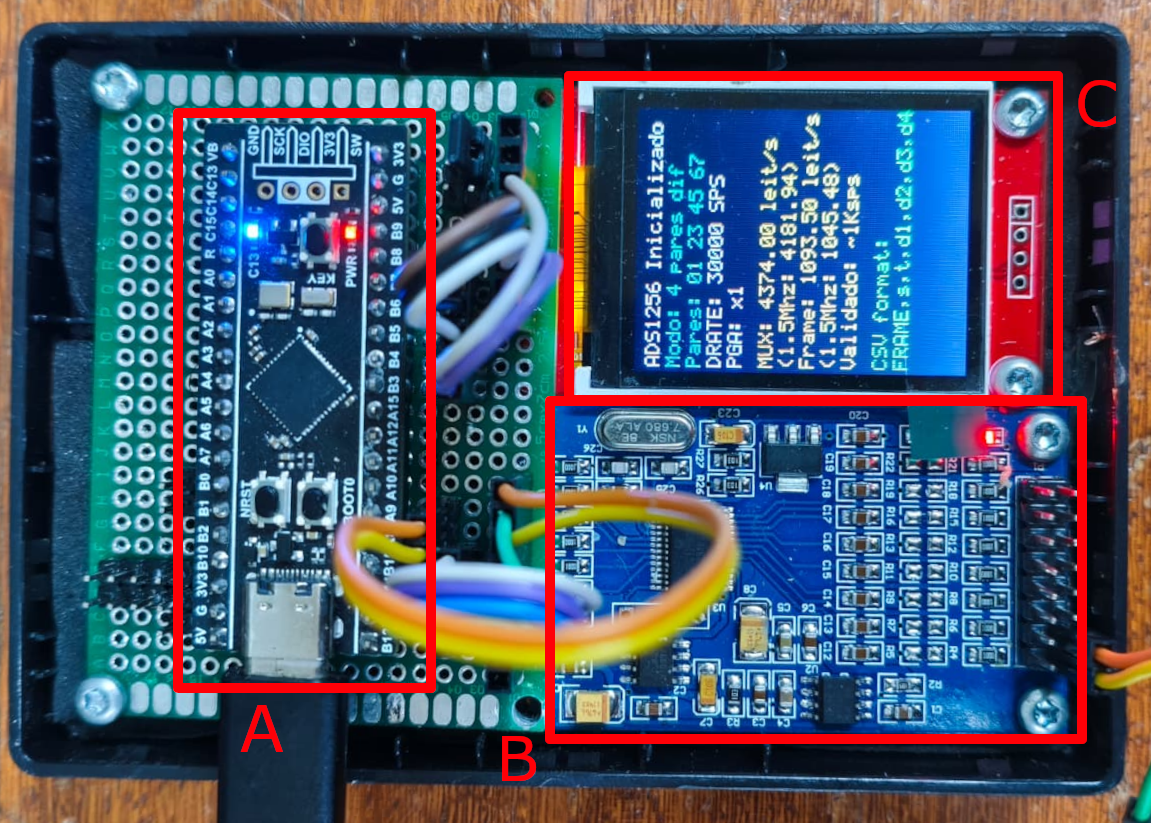
\includegraphics[width=0.75\linewidth]{figuras/montagem_ads1256_stm32_tft.png}
    \caption[Montagem do núcleo de aquisição e controle em placa perfurada]{Montagem do núcleo de aquisição e controle em placa perfurada. Em (A), apresenta-se a STM32 Black Pill, baseada no microcontrolador STM32F411CEU6, responsável pelo controle da aquisição e pela transmissão dos quadros à Raspberry Pi; em (B), o módulo conversor ADS1256, utilizado para digitalização dos sinais analógicos em pares diferenciais; e, em (C), a tela TFT auxiliar de 1,8~polegadas, empregada para exibição local de informações de depuração, como modo de aquisição, pares diferenciais configurados, taxa nominal, ganho programável e formato dos quadros transmitidos.}
    \label{fig:montagem_ads_stm32}
\end{figure}

A camada de processamento e interface foi mantida fisicamente separada do núcleo de aquisição. Essa camada é composta pela Raspberry Pi 3 Model B+, pela tela principal de 7~polegadas e pelo cartão microSD de 64~GB. A Raspberry Pi recebe os quadros transmitidos pela STM32 por meio da porta serial virtual criada pela comunicação USB CDC, executa o software de aquisição e visualização e armazena os dados registrados.

A separação física entre o núcleo de aquisição e a unidade de processamento contribui para organizar a montagem e reduzir a concentração de conexões digitais próximas às entradas analógicas do ADS1256. A Figura~\ref{fig:montagem_raspberry_interface} apresenta a integração entre a Raspberry Pi, a tela principal e o núcleo STM32/ADS1256 durante os testes de bancada.

\begin{figure}[!htb]
    \centering
    \includegraphics[width=0.85\linewidth]{figuras/montagem_raspberry_interface.jpg}
    \caption[Montagem da camada de processamento e interface local do sistema]{Montagem da camada de processamento e interface local do sistema. Em (A), apresenta-se a Raspberry Pi 3 Model B+, responsável pela execução do software de aquisição, visualização e armazenamento; em (B), a tela sensível ao toque de 7~polegadas, utilizada como interface gráfica local; e, em (C), o núcleo de aquisição e controle, composto pela STM32 Black Pill, pelo conversor ADS1256 e pela tela TFT auxiliar. A comunicação entre o núcleo de aquisição e a Raspberry Pi ocorre por USB CDC, enquanto a tela principal recebe o sinal de vídeo por HDMI e envia os eventos de toque por USB.}
    \label{fig:montagem_raspberry_interface}
\end{figure}

As imagens apresentadas nesta subseção têm função documental, mostrando a disposição física dos blocos principais do protótipo. As conexões elétricas, a distribuição dos pares diferenciais e os parâmetros de operação do conversor são descritos nas subseções anteriores, enquanto a montagem de bancada com gerador de funções e osciloscópio é apresentada posteriormente, nos procedimentos de aquisição e validação.

\section{Implementação do firmware}
\label{sec:firmware}

O firmware desenvolvido para a STM32 Black Pill é responsável pelo controle da cadeia de aquisição, pela comunicação com o conversor ADS1256, pela organização das amostras adquiridas e pela transmissão dos dados à Raspberry Pi. Além dessas funções, a implementação também controla uma tela auxiliar, utilizada para apresentar informações de estado, configuração e depuração da aquisição.

A implementação foi desenvolvida em linguagem C com o auxílio do STM32CubeIDE e das bibliotecas de abstração de hardware da STMicroelectronics. O código foi dividido em módulos específicos, buscando separar a lógica de comunicação com os periféricos da coordenação geral da aplicação. Essa organização reduz a concentração de responsabilidades no arquivo principal e facilita a substituição ou alteração individual dos componentes do sistema.

O código-fonte empregado neste trabalho encontra-se disponível em repositório público, incluindo os arquivos de configuração do projeto, os controladores do ADS1256 e da tela ST7735, o módulo de comunicação USB CDC, o módulo de atrasos em microssegundos e os arquivos de compilação para o STM32F411CEU6~\cite{firmware_blackpill_ads1256}.

\subsection{Arquitetura geral do firmware}
\label{subsec:arquitetura_firmware}

A arquitetura do firmware foi estruturada em torno de um arquivo principal e de módulos periféricos especializados. O arquivo \texttt{main.c} concentra a inicialização do microcontrolador, a configuração inicial dos periféricos e a execução do ciclo contínuo de aquisição. As operações específicas de comunicação com os dispositivos externos são implementadas em arquivos próprios, reduzindo o acoplamento entre a lógica principal e os detalhes de cada periférico.

O módulo \texttt{adc\_ads1256} implementa o controlador do conversor A/D. Ele contém as funções de envio de comandos, escrita e leitura de registradores, configuração do multiplexador, controle do ganho programável, seleção da taxa de dados, sincronização das conversões e leitura dos valores quantizados de 24 bits. Também é nesse módulo que se encontra o mapeamento dos pares diferenciais utilizados pelo sistema.

O módulo \texttt{display\_st7735} controla a tela auxiliar. Essa tela é utilizada para apresentar informações de inicialização, estado do ADS1256, taxa configurada, ganho, pares diferenciais ativos e formato dos quadros transmitidos.

O módulo \texttt{microsecond\_clock} fornece uma base de tempo em microssegundos a partir do contador de ciclos do núcleo ARM. Ele inicializa o contador \texttt{DWT->CYCCNT}, acumula os ciclos decorridos e converte esse valor para microssegundos com base na frequência de operação do sistema. Essa referência temporal é utilizada para medir intervalos e organizar o tempo de leitura dos dados do ADS1256.

O módulo \texttt{usb\_cdc\_serial} implementa a transmissão dos dados pela classe USB CDC. Por meio dessa interface, a STM32 é reconhecida pelo sistema operacional da Raspberry Pi como uma porta serial virtual, permitindo que o programa receptor leia os quadros de aquisição de maneira semelhante à leitura de uma porta serial convencional.

Por fim, o módulo \texttt{application\_error} concentra o tratamento de falhas críticas. Quando ocorre uma falha considerada não recuperável, como erro de comunicação com periféricos essenciais ou ausência de resposta do ADS1256 dentro do tempo esperado, a execução normal é interrompida e o LED integrado à placa passa a piscar rapidamente, fornecendo uma indicação visual da falha.

\subsection{Inicialização do microcontrolador e dos periféricos}
\label{subsec:inicializacao_firmware}

A inicialização do firmware ocorre de forma sequencial. Inicialmente, a tabela de vetores de interrupção é ajustada para o endereço \texttt{0x08004000}, utilizado em razão da presença do carregador de inicialização HID da placa Black Pill.

Após esse ajuste, são inicializadas a biblioteca de abstração de hardware, a interface de memória Flash e a base temporal do sistema. Em seguida, são configurados o sistema de clock, as portas de entrada e saída, as interfaces SPI e o periférico USB.

\subsubsection{Configuração do sistema de clock}

O sistema de clock utiliza o oscilador externo da placa como fonte para o circuito PLL. A configuração adotada gera frequência de 96~MHz para o núcleo do STM32F411CEU6 e frequência de 48~MHz para o periférico USB. A escolha de 96~MHz, embora inferior ao limite máximo nominal do microcontrolador, permite gerar adequadamente o clock exigido pela interface USB e mantém capacidade de processamento suficiente para a aquisição multicanal.

O barramento AHB opera na frequência do núcleo, enquanto o barramento APB1 é configurado com divisão por dois e o APB2 permanece sem divisão adicional. Essa configuração define as frequências de operação dos periféricos associados a cada barramento, incluindo as interfaces SPI utilizadas pelo ADS1256 e pela tela auxiliar.

\subsubsection{Configuração das interfaces SPI}

Foram utilizadas duas interfaces SPI independentes. A SPI2 é dedicada à comunicação com o ADS1256, enquanto a SPI3 é utilizada para controle da tela auxiliar. Essa separação evita que a atualização da tela compartilhe diretamente o mesmo barramento empregado na aquisição dos dados.

A SPI2 foi configurada no modo mestre, com transmissão de blocos de 8 bits, envio do bit mais significativo primeiro, polaridade de clock baixa e captura na segunda transição do sinal de clock. A seleção do ADS1256 é controlada por programa, por meio de um pino específico de seleção do dispositivo. Com o divisor configurado, a frequência do clock serial empregado na comunicação com o ADS1256 é de aproximadamente 1,5~MHz.

A SPI3 também opera como mestre, com blocos de 8 bits, sendo utilizada exclusivamente para a comunicação com a tela auxiliar. Essa interface permite apresentar mensagens de estado e informações resumidas sobre a aquisição sem interferir diretamente no barramento utilizado pelo conversor A/D.

\subsubsection{Configuração dos sinais de controle}

Além das linhas SPI, o firmware configura sinais digitais de controle associados ao ADS1256 e à tela auxiliar. No caso do ADS1256, são utilizados o sinal de seleção do dispositivo, o sinal de desligamento e o sinal de dado disponível. Durante a inicialização, esses pinos são colocados em estados conhecidos, evitando acionamentos indevidos.

O terminal de desligamento do ADS1256 é mantido em nível lógico alto, preservando o conversor em operação. O sinal de seleção permanece inicialmente desativado e é acionado apenas durante as transações SPI. O terminal \texttt{DRDY} é configurado como entrada e utilizado para indicar a conclusão de cada conversão.

\subsubsection{Inicialização da interface de comunicação}

A comunicação com a Raspberry Pi é implementada por meio da classe USB CDC. Após a inicialização do periférico USB, o firmware aguarda um intervalo para permitir que o sistema operacional reconheça o dispositivo e disponibilize a porta serial virtual correspondente.

% No sistema operacional da Raspberry Pi, essa interface pode ser acessada como uma porta serial virtual, normalmente associada a um caminho do tipo \texttt{/dev/ttyACM*}. Desse modo, o programa receptor pode utilizar bibliotecas usuais de comunicação serial para receber os dados, embora a transmissão física seja realizada pela interface USB.

\subsection{Driver de comunicação com o ADS1256}
\label{subsec:driver_ads1256}

O driver do ADS1256 foi implementado no módulo \texttt{adc\_ads1256}. Esse módulo concentra as funções de baixo nível necessárias para comunicação com o conversor, incluindo envio de comandos, escrita e leitura de registradores, seleção dos pares diferenciais, espera pelo sinal de dado disponível e leitura dos valores digitalizados.

\subsubsection{Comandos e acesso aos registradores}

O acesso ao ADS1256 é realizado por meio de comandos enviados pela interface SPI. O firmware implementa comandos de reinicialização, interrupção do modo de leitura contínua, escrita de registradores, leitura de registradores, sincronização, retomada da conversão, leitura de dados e autocalibração.

A escrita de registradores é utilizada para configurar o multiplexador de entrada, o ganho programável e a taxa de saída de dados. Após cada operação de escrita ou comando sensível à temporização, são aplicados pequenos atrasos em microssegundos, de modo a respeitar os tempos mínimos exigidos pelo conversor.

A leitura de registradores é utilizada como etapa de verificação. Após configurar o multiplexador, o firmware lê o valor do registrador correspondente e compara o resultado com o valor esperado. Caso seja encontrada divergência, uma mensagem de erro é enviada pela interface USB CDC, uma indicação é apresentada na tela auxiliar e a execução é direcionada ao tratamento de falha.

\subsubsection{Reinicialização, autocalibração e verificação}

A inicialização do ADS1256 começa com a liberação do sinal de seleção e a manutenção do terminal de desligamento em nível lógico alto. Em seguida, o conversor é reinicializado por comando SPI, uma vez que o módulo utilizado não expõe um pino físico de reinicialização dedicado.

Após a reinicialização, o firmware aguarda o sinal \texttt{DRDY}, indicando que o conversor concluiu sua etapa interna de estabilização. Caso o sinal não seja observado dentro do intervalo previsto, o firmware transmite uma mensagem de erro e interrompe a execução normal.

Com o conversor ativo, o firmware envia o comando para interromper qualquer modo de leitura contínua previamente habilitado. Em seguida, são configurados os registradores do multiplexador, do ganho programável e da taxa de saída de dados. Após essa configuração, o comando de autocalibração é executado, e o firmware novamente aguarda a indicação de conclusão por meio do sinal \texttt{DRDY}.

\subsection{Aquisição e chaveamento dos canais}
\label{subsec:aquisicao_chaveamento_firmware}

A aquisição é organizada em quadros. Cada quadro contém uma amostra de cada um dos quatro pares diferenciais configurados. Assim, a cada ciclo completo de leitura, são obtidos quatro valores: \texttt{d1}, \texttt{d2}, \texttt{d3} e \texttt{d4}. Esses valores correspondem, respectivamente, aos pares AIN0/AIN1, AIN2/AIN3, AIN4/AIN5 e AIN6/AIN7.

\subsubsection{Sincronização pelo sinal DRDY}

A sincronização das leituras utiliza o terminal \texttt{DRDY} do ADS1256. Esse sinal indica que uma nova conversão está disponível. Enquanto \texttt{DRDY} permanece em nível lógico alto, o firmware aguarda; quando o sinal muda para o estado ativo, a leitura pode ser realizada.

Essa estratégia evita que o microcontrolador leia o conversor antes da conclusão da conversão. Na inicialização e na autocalibração, a espera por \texttt{DRDY} possui tempo máximo definido, permitindo detectar falhas de resposta. Durante o ciclo normal de aquisição, a rotina aguarda a disponibilização dos dados antes de prosseguir com a leitura.

\subsubsection{Sequência de multiplexação}

A sequência de multiplexação percorre os quatro pares diferenciais na ordem AIN0/AIN1, AIN2/AIN3, AIN4/AIN5 e AIN6/AIN7. O firmware utiliza uma lógica encadeada: após uma conversão estar disponível para o canal atual, o próximo canal é selecionado, a conversão é sincronizada e o valor anteriormente disponibilizado é lido. Essa forma de operação reduz o tempo ocioso entre leituras e permite manter uma varredura contínua dos quatro pares diferenciais.

\subsubsection{Leitura das palavras de 24 bits}

Cada leitura do ADS1256 retorna três bytes, que representam uma palavra digital de 24 bits em complemento de dois. Após o envio do comando de leitura, o firmware gera os pulsos de clock necessários pela interface SPI e recebe os três bytes correspondentes ao valor convertido.

O valor bruto recebido é inicialmente reconstruído por concatenação dos três bytes. Em seguida, é realizada a extensão de sinal para 32 bits, permitindo armazenar corretamente valores positivos e negativos em uma variável inteira com sinal. Esse procedimento é necessário porque o conversor fornece resultados assinados em 24 bits, enquanto o microcontrolador manipula esses valores em variáveis de 32 bits.

\subsection{Organização das amostras e formação dos quadros}
\label{subsec:organizacao_quadros_firmware}

Após a leitura dos quatro pares diferenciais, as amostras são organizadas em um vetor local com quatro posições. Cada posição do vetor corresponde a um par diferencial específico, preservando a ordem definida no mapeamento de canais.

Além dos valores brutos do ADS1256, cada quadro recebe um número sequencial e uma marca temporal em microssegundos. O número sequencial é incrementado a cada quadro transmitido, permitindo ao programa receptor identificar eventuais saltos na sequência. A marca temporal é obtida a partir da base de tempo fornecida pelo módulo \texttt{microsecond\_clock}, por meio da função \texttt{MicrosecondClock\_Now()}, que retorna o tempo acumulado em microssegundos desde a inicialização do contador.

\subsection{Transmissão dos dados por USB CDC}
\label{subsec:transmissao_usb_cdc}

A transmissão dos dados é realizada pela classe USB CDC, que permite ao microcontrolador aparecer para a Raspberry Pi como uma porta serial virtual. Essa escolha simplifica a integração com o programa de recepção, pois permite utilizar bibliotecas usuais de leitura serial no ambiente Linux.

\subsection{Interface local de depuração}
\label{subsec:interface_depuracao_firmware}

A tela TFT ST7735 conectada à STM32 é utilizada como interface local de depuração. Durante a inicialização, ela apresenta mensagens relacionadas ao estado do ADS1256, ao modo de aquisição, aos pares diferenciais configurados, à taxa nominal selecionada, ao ganho programável e ao formato dos quadros transmitidos.

Essa interface auxiliar permite verificar rapidamente se o microcontrolador inicializou o conversor e se os parâmetros principais foram aplicados. Também facilita a identificação de falhas durante testes de bancada, especialmente quando o sistema ainda não está conectado à Raspberry Pi ou quando a comunicação USB CDC não foi iniciada corretamente.

\subsection{Tratamento de falhas}
\label{subsec:tratamento_falhas_firmware}

O tratamento de falhas da versão atual concentra-se em condições críticas de inicialização e comunicação com os periféricos. As chamadas às funções da biblioteca de abstração de hardware são verificadas, e uma falha nessas chamadas conduz à rotina de erro da aplicação.

No caso específico do ADS1256, o firmware verifica se o sinal \texttt{DRDY} é observado após o comando de reinicialização e após a autocalibração. Caso o sinal não seja detectado dentro do tempo máximo definido, uma mensagem de erro é transmitida pela interface USB CDC e a execução normal é interrompida.

Também é realizada a leitura de retorno do registrador do multiplexador após sua configuração inicial. Se o valor lido for diferente do valor esperado, o firmware transmite uma mensagem de erro, apresenta a falha na tela auxiliar e aciona o tratamento de erro.

Quando uma falha crítica é identificada, a rotina de erro desabilita a execução normal e utiliza o LED integrado da Black Pill como indicação visual. Esse comportamento permite distinguir uma falha de inicialização de uma simples ausência de dados no programa receptor.

\section{Implementação do software de aquisição, processamento e visualização}
\label{sec:software}

O software executado na Raspberry Pi foi desenvolvido para receber, processar, visualizar e armazenar continuamente os dados enviados pela STM32. A aplicação atua como a camada de mais alto nível da plataforma, recebendo os quadros multicanais transmitidos pelo firmware, validando sua estrutura, separando as amostras por canal e disponibilizando os sinais para visualização em forma online.

Foram utilizadas a linguagem Python e as bibliotecas PyQt5, para construção da
interface gráfica, PyQtGraph, para representação dos sinais, NumPy e SciPy, para
manipulação numérica e processamento digital, h5py, para armazenamento das sessões e PySerial, para acesso à comunicação serial. A escolha dessas ferramentas permitiu reunir, em uma mesma aplicação, os recursos de aquisição, processamento, visualização e gerenciamento
das sessões.

O código-fonte da aplicação encontra-se disponível em repositório público, contendo os módulos responsáveis pela leitura da comunicação serial virtual, interpretação dos quadros, gerenciamento da aquisição, armazenamento das sessões, processamento digital, visualização gráfica, exportação e validação automatizada~\cite{software_processamento_biomedico}.

\subsection{Arquitetura geral do software}
\label{subsec:arquitetura_software}

A arquitetura do software foi organizada em camadas, com separação entre aquisição, armazenamento, processamento e interface gráfica. Essa divisão foi adotada para evitar que a visualização dos sinais limitasse a aquisição ou comprometesse a gravação dos dados. Assim, a atualização dos gráficos, a aplicação de filtros e a inspeção visual dos registros são tratadas como produtos derivados da aquisição, e não como condição para que os dados sejam preservados.

A estrutura lógica do software pode ser sintetizada como mostrado na Figura~\ref{fig:fluxo-aquisicao}. O fluxo principal da aplicação inicia-se na leitura da porta serial virtual associada à STM32. As linhas recebidas são encaminhadas a um analisador de quadros, responsável por verificar o cabeçalho, a quantidade de campos, os valores numéricos, o número sequencial e a marca temporal. Os quadros aceitos seguem simultaneamente para uma memória circular, utilizada pela interface de visualização, e para o serviço de gravação contínua.

\begin{figure}[htbp]
    \centering

\begin{tikzpicture}[
        block/.style={
            rectangle,
            draw,
            rounded corners,
            align=center,
            font=\small,
            minimum width=3.0cm,
            minimum height=0.8cm
        },
        arrow/.style={
            -{Latex},
            thick
        },
        node distance=1.1cm and 1.3cm
    ]
    
        % Primeira linha
        \node[block] (stm32) {STM32};
        
        \node[block, right=of stm32] (serial) {Leitor serial +\\analisador de quadros};
        
        \node[block, right=of serial] (aquisicao) {Serviço de\\aquisição};
        
        % Segunda linha: fluxo para processamento
         
        \node[block, below=1.2cm of stm32] (gui) {Interface\\gráfica};
        
        \node[block, right=of gui] (processamento) {Processamento};
        
        \node[block, right=of processamento] (memoria) {Memória\\circular};
        
        % Terceira linha: fluxo para gravação
        \node[block, below=1.0cm of processamento] (hdf5) {Arquivo\\HDF5};
        
        \node[block, right=of hdf5] (gravacao) {Serviço de\\gravação};
        
        % Conexões da primeira linha
        \draw[arrow] (stm32) -- (serial);
        \draw[arrow] (serial) -- (aquisicao);
        
        % % Ramificações a partir do serviço de aquisição
        % \draw[arrow] (aquisicao.east) |- (memoria.east);
        % \draw[arrow] (aquisicao.east) |- (gravacao.east);
               
        % Ponto de ramificação
        \coordinate (ramo) at ($(aquisicao.east) + (0.45cm,0)$);
        
        % Ramificações a partir do serviço de aquisição
        \draw[thick] (aquisicao.east) -- (ramo);
        \draw[arrow] (ramo) |- (memoria.east);
        \draw[arrow] (ramo) |- (gravacao.east);
        
        % Fluxos inferiores
        \draw[arrow] (memoria) -- (processamento);
        \draw[arrow] (processamento) -- (gui);
        
        \draw[arrow] (gravacao) -- (hdf5);
    
    \end{tikzpicture}
    
    \caption[Fluxo de aquisição, armazenamento e processamento dos dados]{Arquitetura funcional do fluxo de aquisição, processamento e armazenamento de dados. O STM32 envia os dados por comunicação serial para o módulo de leitura e análise de quadros. Em seguida, o serviço de aquisição distribui os dados para dois caminhos: a memória circular, que disponibiliza as amostras ao processamento e posteriormente à interface gráfica, e o serviço de gravação, que persiste os dados em um arquivo HDF5.}
    \label{fig:fluxo-aquisicao}
\end{figure}

A memória circular armazena apenas a janela necessária à visualização ao vivo. Dessa forma, a quantidade de pontos exibida no gráfico pode ser limitada sem reduzir a extensão da sessão registrada. A gravação, por sua vez, ocorre de maneira independente, por meio de uma fila limitada e de um serviço de escrita em arquivo. Essa separação permite que a interface opere com uma janela reduzida, enquanto a sessão completa permanece registrada em disco.

\subsection{Configuração da sessão e dos canais}
\label{subsec:configuracao_sessao_software}

Antes do início da aquisição, o usuário configura a sessão por meio da interface gráfica. Nessa etapa, são definidos a porta de comunicação, a taxa base esperada, a janela temporal de visualização, a tensão de referência do ADS1256, o ganho global do amplificador programável e a ordem dos canais recebidos.

A ordem configurada na interface deve corresponder à ordem dos valores transmitidos pelo firmware. Cada canal pode ser configurado para visualização em contagem bruta ou em tensão diferencial na entrada do conversor. A contagem bruta preserva diretamente o valor assinado produzido pelo ADS1256, enquanto a tensão diferencial é calculada a partir da tensão de referência e do ganho programável informados na configuração. Essa seleção altera a grandeza utilizada pela interface e pelo processamento, mas não modifica o dado bruto armazenado.

A configuração também permite salvar predefinições de uso, facilitando a repetição de ensaios com a mesma ordem de canais, os mesmos parâmetros de conversão e as mesmas condições de visualização.

\subsection{Recepção e validação dos quadros}
\label{subsec:recepcao_validacao_software}

A comunicação entre a STM32 e a Raspberry Pi é acessada pelo software como uma porta serial, embora a transmissão física seja realizada por USB CDC. O leitor serial executa em uma linha de execução separada da interface gráfica, impedindo que a espera por dados bloqueie a interação do usuário com a aplicação.

O protocolo de comunicação utiliza linhas textuais no formato:

\begin{verbatim}
    FRAME,<sequence_id>,<timestamp_us>,<v0>,<v1>,...,<vN>
\end{verbatim}

O campo \texttt{FRAME} identifica o início de um quadro válido. O campo \texttt{sequence\_id} representa o número sequencial do quadro, enquanto o campo \texttt{timestamp\_us} representa a marca temporal associada ao ciclo de varredura. Os campos \texttt{v0} a \texttt{vN} armazenam os valores brutos dos canais, na ordem definida na interface.

O analisador de quadros verifica se a linha recebida possui cabeçalho válido, quantidade adequada de campos e valores numéricos compatíveis com os limites esperados. Linhas incompletas, campos ausentes, valores inválidos e estruturas incompatíveis são contabilizados como erros de protocolo e não são encaminhados ao processamento normal.

Além da validação estrutural, o software acompanha o comportamento do número sequencial e da marca temporal. A partir desses campos, são identificados quadros ausentes, duplicados, fora de ordem e regressões temporais. Essas informações são apresentadas como diagnóstico da comunicação, permitindo avaliar se a aquisição está ocorrendo de forma contínua e compatível com a taxa esperada.

\subsection{Armazenamento das aquisições}
\label{subsec:armazenamento_software}

O armazenamento das sessões foi implementado em arquivos HDF5. Durante a gravação, a sessão é criada inicialmente com extensão temporária e, ao ser finalizada corretamente, é consolidada com extensão definitiva. Essa estratégia reduz o risco de interpretar como completa uma sessão interrompida durante a escrita.

A estrutura principal do arquivo contém os conjuntos de dados referentes ao número sequencial, à marca temporal e aos valores brutos recebidos. Os valores dos canais são armazenados em uma matriz extensível, na qual cada linha corresponde a um quadro multicanal e cada coluna corresponde a um canal configurado.

O armazenamento preserva as contagens brutas recebidas do microcontrolador. A conversão para tensão, os filtros digitais, as métricas e o espectro são tratados como produtos derivados, podendo ser recalculados posteriormente a partir dos dados originais.

Os arquivos de sessão também armazenam metadados relevantes, como configuração da comunicação, ordem dos canais, tensão de referência, ganho, seleção de visualização por canal, filtros ativos, estado de encerramento da sessão e diagnósticos de comunicação. Esses metadados permitem reabrir a sessão posteriormente com informações suficientes para sua interpretação.

\subsection{Conversão das contagens do ADS1256}
\label{subsec:conversao_ads_software}

O microcontrolador transmite a contagem assinada de 24 bits produzida pelo ADS1256. Quando o usuário seleciona a visualização em tensão, o software converte essa contagem para tensão diferencial na entrada do conversor, considerando o modo diferencial de operação, a tensão de referência e o ganho global do amplificador programável.

A faixa nominal de entrada é definida por

\begin{equation}
    V_{\mathrm{FS}} =
    \pm \frac{2V_{\mathrm{REF}}}{G},
    \label{eq:vfs_ads1256_software}
\end{equation}

\noindent
em que $V_{\mathrm{REF}}$ é a tensão de referência e $G$ é o ganho programado no ADS1256.

Como o resultado do conversor é representado em complemento de dois com 24 bits, os extremos positivo e negativo possuem quantidades ligeiramente diferentes de níveis. Por esse motivo, o software trata separadamente as contagens positivas e negativas. Para contagens maiores ou iguais a zero, a tensão é calculada por

\begin{equation}
    V =
    \frac{\mathrm{count}\cdot V_{\mathrm{FS}}}{8388607}.
    \label{eq:conversao_ads_positiva}
\end{equation}

\noindent
Para contagens negativas, utiliza-se

\begin{equation}
    V =
    \frac{\mathrm{count}\cdot V_{\mathrm{FS}}}{8388608}.
    \label{eq:conversao_ads_negativa}
\end{equation}

\noindent
A tensão obtida corresponde à tensão diferencial na entrada do ADS1256, isto é, à diferença entre os terminais positivo e negativo do par selecionado.

\subsection{Processamento dos sinais}
\label{subsec:processamento_sinais_software}

O processamento digital é aplicado sobre o sinal base selecionado para cada canal, que pode corresponder à contagem bruta ou à tensão diferencial. A aplicação disponibiliza filtros configuráveis para remoção de linha de base, remoção de componente contínua, filtragem passa-altas, rejeição de 60~Hz, filtragem passa-faixa, filtragem passa-baixas, média móvel e cálculo de envelope.

Além dos filtros, o software calcula métricas básicas dos sinais apresentados, como média, valor eficaz, mínimo e máximo. Essas métricas auxiliam a inspeção do comportamento dos canais durante a aquisição e podem indicar saturação, deslocamento excessivo de nível, perda de contato ou aumento de ruído.

A análise espectral é realizada por meio da Transformada Rápida de Fourier. O espectro é calculado de forma unilateral, permitindo observar a frequência dominante, a magnitude de pico e a resolução espectral associada ao trecho selecionado. A visualização espectral pode ser aplicada ao sinal base ou ao sinal processado, conforme a escolha do usuário.

Para reduzir o custo computacional, o processamento completo é aplicado preferencialmente ao canal visível na interface. Assim, apenas a aba selecionada é convertida, filtrada, analisada e redesenhada continuamente. Essa escolha preserva a responsividade da interface e evita processamento desnecessário de canais que não estão sendo visualizados naquele instante.

\subsection{Sessões armazenadas e exportação}
\label{subsec:sessoes_exportacao_software}

Além da visualização ao vivo, a aplicação permite reabrir sessões previamente gravadas. Nessa etapa, o usuário pode selecionar um arquivo, verificar sua integridade, definir o trecho temporal de interesse e limitar a quantidade de pontos carregados para visualização. Essa abordagem evita que sessões longas sejam carregadas integralmente em memória apenas para inspeção gráfica.

Quando a sessão contém mais pontos do que o limite visual definido, a redução é aplicada apenas para exibição. O arquivo HDF5 permanece inalterado, preservando todos os quadros registrados. Essa distinção é importante porque a visualização reduzida não deve ser confundida com perda ou reamostragem permanente dos dados.

O software também permite exportar a sessão completa para CSV em blocos. Essa funcionalidade facilita a análise posterior em outros ambientes, como Python ou MATLAB, sem depender exclusivamente da interface gráfica desenvolvida no projeto.


\section{Ensaios de Validação da Arquitetura Desenvolvida}
\label{sec:procedimentos_aquisicao}

Os ensaios de validação foram organizados para verificar o funcionamento da cadeia completa de aquisição, desde a entrada analógica do ADS1256 até a recepção, visualização e armazenamento dos dados na Raspberry Pi. A validação foi dividida em duas etapas principais. A primeira compreendeu ensaios de bancada com sinais conhecidos, gerados por gerador de funções e observados por osciloscópio. A segunda correspondeu à aquisição de sinais fisiológicos, contemplando dois canais de ECG e um canal de PPG por meio dos módulos específicos integrados à plataforma.

Nos ensaios de bancada, os sinais foram aplicados ao sistema desenvolvido e simultaneamente observados no osciloscópio. Como o osciloscópio utilizado dispõe de dois canais de entrada, os sinais foram adquiridos em pares. Essa organização permitiu que cada sinal gerado fosse acompanhado por um canal do osciloscópio, mantendo uma referência visual e paramétrica para a forma de onda aplicada.

A validação foi realizada por meio dos parâmetros configurados no gerador de funções, das métricas apresentadas pelo osciloscópio e das grandezas extraídas dos arquivos registrados pelo sistema, como frequência estimada, amplitude, comportamento temporal e conteúdo espectral.

Durante os ensaios, foram registrados pares de sinais com diferentes formas de onda, amplitudes e frequências. Essa diversidade foi adotada para submeter a arquitetura a situações distintas de aquisição, incluindo sinais de baixa frequência, sinais com transições abruptas, sinais com conteúdo harmônico, sinais em frequência mais elevada e sinais com composição espectral mais complexa.

\subsection{Ensaios com sinais conhecidos}
\label{subsec:sinais_conhecidos}

Os ensaios com sinais conhecidos foram realizados por meio da aplicação de formas de onda produzidas pelo gerador de funções Politerm POL-40 às entradas diferenciais do ADS1256. Cada sinal aplicado ao sistema desenvolvido também foi encaminhado a um canal do osciloscópio, utilizado como referência experimental para conferência da forma de onda e de métricas como frequência, amplitude e nível médio.

Em todos os casos, os sinais foram aplicados aos pares diferenciais selecionados do ADS1256, respeitando-se os limites de tensão de entrada e de modo comum do conversor. O gerador de funções, o osciloscópio e o sistema de aquisição compartilharam a referência elétrica necessária à medição em bancada. Antes do início de cada registro, foram conferidas no osciloscópio a forma de onda, a frequência, a amplitude e a componente contínua configuradas no gerador. A montagem experimental utilizada nesses ensaios é apresentada na Figura~\ref{fig:montagem_bancada_validacao}.

\begin{figure}[!htb]
    \centering
    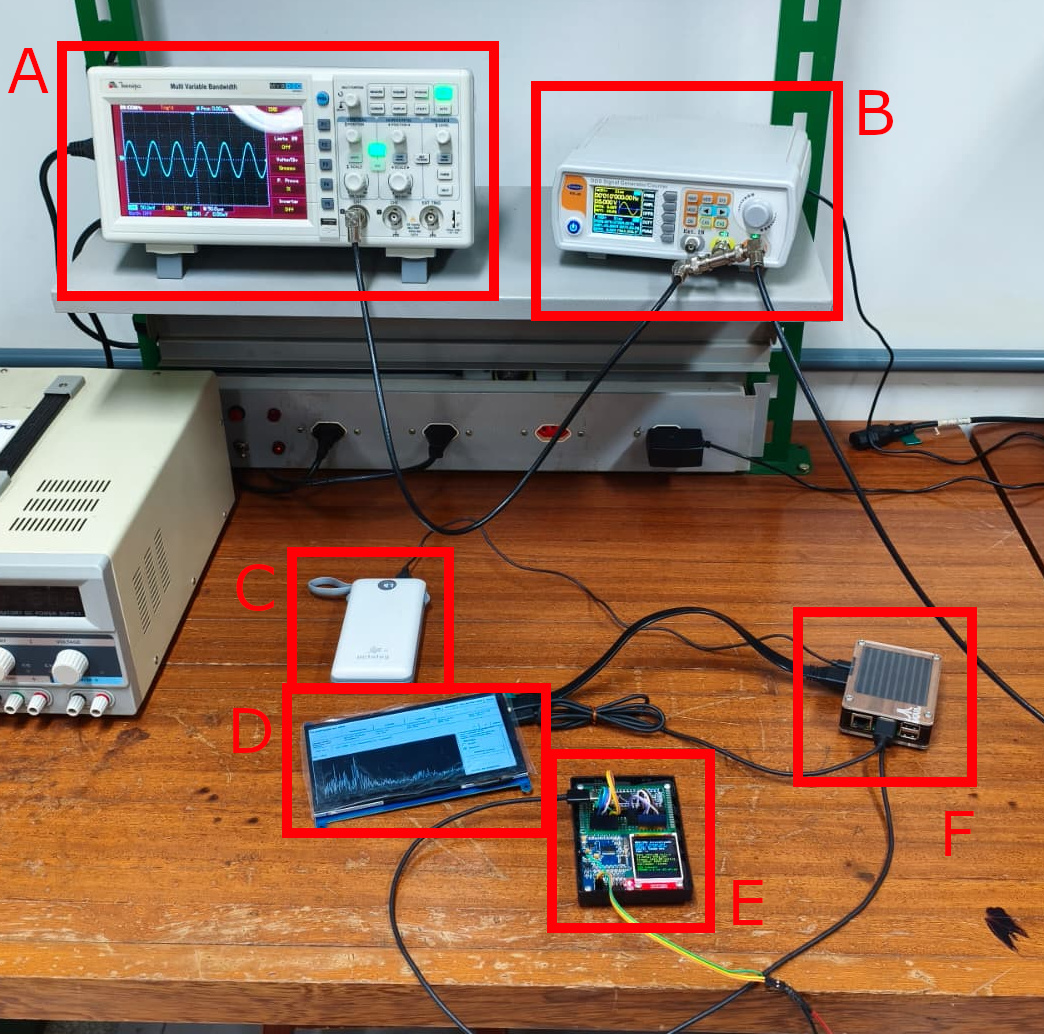
\includegraphics[width=0.92\textwidth]
    {figuras/montagem_bancada_validacao.jpeg}
    \caption[Montagem experimental utilizada nos ensaios de bancada]{Montagem experimental utilizada nos ensaios de bancada com sinais conhecidos, composta pelo osciloscópio, gerador de funções, fonte de alimentação, sistema de aquisição baseado no ADS1256, interface local de visualização e Raspberry Pi responsável pela recepção e pelo armazenamento dos dados.}
    \label{fig:montagem_bancada_validacao}
\end{figure}

Foram utilizadas formas de onda senoidais, quadradas, multitom e sinc. As senoides foram empregadas como referência inicial por apresentarem uma componente espectral dominante. As ondas quadradas foram utilizadas para avaliar a resposta da cadeia de aquisição diante de transições abruptas e maior conteúdo harmônico. Os sinais multitom e sinc foram incluídos para verificar a resposta do sistema diante de conteúdo espectral mais composto.

Conforme apresentado na Tabela~\ref{tab:sinais_bancada_adquiridos}, nem todos os sinais possuem a mesma função na validação. Os sinais senoidais são mais adequados para verificar frequência e amplitude de forma direta. As ondas quadradas permitem observar a resposta a harmônicos e transições. Já os sinais multitom e sinc são mais úteis para avaliar a representação espectral da cadeia de aquisição.

\begin{table}[!htb]
    \centering
    \caption{Pares de sinais conhecidos adquiridos nos ensaios de bancada.}
    \label{tab:sinais_bancada_adquiridos}
    \renewcommand{\arraystretch}{1.2}
    \begin{tabularx}{\textwidth}{p{4.2cm}p{4.2cm}X}
        \hline
        \textbf{Primeiro sinal} &
        \textbf{Segundo sinal} &
        \textbf{Finalidade do ensaio} \\
        \hline

        Senoidal, 100~Hz, amplitude 2~V &
        Senoidal, 450~Hz, amplitude 2~V &
        Verificar o comportamento da aquisição em frequências mais elevadas, especialmente em relação à taxa efetiva de amostragem. \\

        Quadrada, 5~Hz, amplitude 5~V &
        Quadrada, 50~Hz, amplitude 5~V &
        Avaliar a preservação dos patamares, das bordas e das componentes harmônicas de ondas quadradas em diferentes frequências. \\

        Multitom, 50~Hz, amplitude 5~V &
        Sinc, 50~Hz, amplitude 5~V &
        Avaliar a representação de sinais com conteúdo espectral composto e distribuição de energia em múltiplas componentes. \\
        \hline
    \end{tabularx}
\end{table}

Nos ensaios com dois sinais simultâneos, cada saída do gerador foi associada a um canal do osciloscópio e a um par diferencial do ADS1256. A associação entre os canais foi registrada na configuração da sessão, permitindo identificar posteriormente qual sinal corresponde a cada coluna do arquivo armazenado pelo software de aquisição.

Os arquivos gerados pelo sistema foram salvos em formato digital e posteriormente utilizados para análise temporal e espectral. A análise temporal considerou grandezas como valor máximo, valor mínimo, amplitude pico a pico, valor médio, período e frequência estimada. A análise espectral foi realizada por meio da Transformada Rápida de Fourier, permitindo verificar a posição da componente fundamental, a presença de harmônicos esperados e a ocorrência de componentes espúrias.

As capturas de tela do osciloscópio foram utilizadas como registro documental das condições de bancada e das métricas apresentadas pelo instrumento. Dessa forma, o osciloscópio serviu como referência visual e paramétrica, enquanto os arquivos adquiridos pelo sistema foram utilizados para os cálculos quantitativos detalhados.

\subsection{Aquisição de sinais fisiológicos}
\label{subsec:aquisicao_fisiologica}

Após os ensaios com sinais conhecidos, foram realizadas aquisições de dois canais de ECG e de um canal de PPG. Essa etapa teve como objetivo verificar o funcionamento da plataforma diante de sinais fisiológicos reais, sujeitos a variações de contato, interferência eletromagnética, artefatos de movimento e instabilidade da linha de base.

Os sinais de ECG foram adquiridos por dois módulos baseados no AD8232, alimentados em 3,3~V. Cada módulo foi associado a um canal independente do sistema, permitindo o registro simultâneo de dois sinais cardíacos. As saídas analógicas dos módulos foram encaminhadas aos pares diferenciais AIN0/AIN1 e AIN2/AIN3 do ADS1256. O sinal de PPG foi adquirido com o Pulse Sensor Amped, alimentado em 5~V. A saída analógica do sensor foi conectada ao par diferencial AIN4/AIN5 do ADS1256.

Durante as aquisições fisiológicas, os sinais foram visualizados pela interface local executada na Raspberry Pi e armazenados para análise posterior. A avaliação desses registros concentrou-se na identificação das estruturas esperadas dos sinais, na estabilidade da aquisição e na presença de ruídos ou artefatos. No caso do ECG, foram observados os complexos QRS, a linha de base e a interferência de rede. No caso do PPG, foram observados a componente pulsátil, a regularidade dos pulsos e a sensibilidade a movimento e variações de contato.

Essas aquisições tiveram caráter funcional e instrumental, não constituindo validação clínica ou diagnóstica do sistema. O objetivo foi verificar se a arquitetura desenvolvida é capaz de registrar sinais fisiológicos compatíveis com sua natureza esperada e disponibilizá-los para visualização e análise posterior.

\section{Estratégia de validação}
\label{sec:estrategia_validacao}

A estratégia de validação foi dividida em duas abordagens complementares. Para os sinais conhecidos gerados em bancada, a validação foi realizada por comparação paramétrica entre os valores configurados no gerador de funções, as métricas observadas no osciloscópio e as grandezas extraídas dos arquivos registrados pelo sistema desenvolvido. Para os sinais fisiológicos, a avaliação teve caráter funcional e instrumental, restrita à verificação de que os módulos de aquisição produziram sinais compatíveis com os fenômenos esperados e de que a arquitetura foi capaz de adquiri-los, separá-los por canal, visualizá-los e armazená-los corretamente.

O osciloscópio foi utilizado como instrumento de referência experimental para conferência visual das formas de onda e leitura de métricas, como frequência, período e amplitude. A análise quantitativa principal foi realizada sobre os dados armazenados pelo sistema desenvolvido. Esses registros permitiram calcular frequência estimada, amplitude pico a pico, valor médio, componentes espectrais e indicadores de continuidade da aquisição. As capturas de tela do osciloscópio foram utilizadas como documentação das condições de bancada e como referência independente para as métricas exibidas pelo instrumento.

\subsection{Validação no domínio do tempo}
\label{subsec:validacao_tempo}

No domínio do tempo, os sinais adquiridos pelo sistema foram avaliados quanto à forma de onda, frequência estimada, período, amplitude pico a pico, componente contínua, estabilidade da linha de base e presença de saturação. Esses parâmetros foram extraídos dos arquivos registrados pela plataforma e comparados com os valores configurados no gerador de funções e com as métricas apresentadas pelo osciloscópio.

A frequência de cada sinal foi estimada a partir dos dados adquiridos pelo sistema, utilizando a identificação de ciclos consecutivos no domínio do tempo ou, quando mais adequado, a frequência da componente dominante obtida na análise espectral. O erro relativo de frequência foi calculado por

\begin{equation}
    \varepsilon_f =
    \frac{\left|f_{\mathrm{sistema}}-f_{\mathrm{ref}}\right|}
    {f_{\mathrm{ref}}}
    \times 100\%,
    \label{eq:erro_frequencia}
\end{equation}

\noindent
em que $f_{\mathrm{sistema}}$ representa a frequência estimada a partir do registro do sistema e $f_{\mathrm{ref}}$ corresponde à frequência configurada no gerador de funções ou indicada pelo osciloscópio.

A amplitude foi avaliada preferencialmente pela tensão pico a pico, calculada a partir dos valores máximo e mínimo do trecho analisado. Quando os dados foram convertidos para tensão diferencial na entrada do ADS1256, o erro relativo de amplitude foi calculado por

\begin{equation}
    \varepsilon_A =
    \frac{\left|A_{\mathrm{sistema}}-A_{\mathrm{ref}}\right|}
    {A_{\mathrm{ref}}}
    \times 100\%,
    \label{eq:erro_amplitude}
\end{equation}

\noindent
em que $A_{\mathrm{sistema}}$ representa a amplitude pico a pico estimada a partir dos dados registrados e $A_{\mathrm{ref}}$ corresponde à amplitude configurada no gerador ou medida pelo osciloscópio.

Para sinais senoidais, a validação temporal concentrou-se na regularidade dos ciclos, na coerência da frequência, na amplitude pico a pico e na ausência de deformações perceptíveis. Para sinais quadrados, foram observados os patamares, as bordas de subida e descida e a preservação do período. Para sinais triangulares, foram avaliadas a linearidade aproximada das rampas, a simetria entre subida e descida e a preservação dos vértices. Nos sinais de maior frequência, a interpretação considerou a taxa efetiva de amostragem, pois a redução do número de amostras por ciclo afeta diretamente a representação temporal.

Também foi verificada a ocorrência de saturação. Essa verificação foi feita pela observação dos valores máximo e mínimo registrados e pela inspeção da forma de onda. Trechos com achatamento nos extremos, permanência prolongada em valores limite ou perda evidente da forma esperada foram interpretados como indícios de saturação ou inadequação da faixa de entrada.

\subsection{Validação no domínio da frequência}
\label{subsec:validacao_frequencia}

No domínio da frequência, os sinais registrados pelo sistema foram analisados por meio da Transformada Rápida de Fourier. Antes do cálculo da FFT, os trechos selecionados foram submetidos à remoção da componente média, de modo a reduzir a influência da componente de frequência nula. Quando necessário, também foi aplicada uma janela temporal para reduzir os efeitos de descontinuidade nas bordas do segmento analisado.

A resolução espectral foi determinada por

\begin{equation}
    \Delta f = \frac{f_s}{N},
    \label{eq:resolucao_espectral}
\end{equation}

\noindent
em que $f_s$ representa a taxa efetiva de amostragem do canal analisado e $N$ corresponde ao número de amostras utilizadas na FFT.

Para os sinais senoidais, verificou-se se a componente dominante do espectro coincidia com a frequência configurada no gerador de funções. Para as ondas quadradas, além da frequência fundamental, foram observadas as harmônicas ímpares esperadas, respeitando-se o limite imposto pela frequência de Nyquist. Nos sinais multitom e sinc, a avaliação concentrou-se na distribuição das componentes espectrais e na coerência entre o formato esperado e o espectro obtido.

A frequência de Nyquist foi considerada em todos os ensaios, especialmente naqueles com frequências mais elevadas. Para uma taxa efetiva de amostragem $f_s$, a maior frequência representável sem ambiguidade é dada por

\begin{equation}
    f_N = \frac{f_s}{2}.
    \label{eq:nyquist_validacao}
\end{equation}

\noindent
Assim, sinais próximos desse limite, como a senoide de 450~Hz quando adquirida com taxa efetiva próxima de 1~kS/s, foram tratados como ensaios de limite da arquitetura. Nesses casos, espera-se menor quantidade de amostras por ciclo, maior sensibilidade a variações temporais e maior possibilidade de deformação na representação temporal.

A análise espectral também permitiu identificar componentes não esperadas, especialmente interferências concentradas em 60~Hz e em seus múltiplos. Essas componentes foram interpretadas como indícios de acoplamento com a rede elétrica ou de ruídos introduzidos pela montagem, pelos cabos ou pelas referências elétricas compartilhadas.

\subsection{Validação da aquisição multicanal}
\label{subsec:validacao_multicanal}

Além da análise individual de cada forma de onda, a validação também considerou a capacidade do sistema de adquirir múltiplos sinais no mesmo registro. Essa verificação é necessária porque o ADS1256 foi utilizado em modo multiplexado, no qual os pares diferenciais são lidos sequencialmente. Portanto, os canais de um mesmo quadro representam amostras obtidas em instantes sucessivos, e não amostras fisicamente simultâneas.

A organização dos canais foi avaliada pela correspondência entre os sinais aplicados aos pares diferenciais e as colunas armazenadas no arquivo de aquisição. Em cada ensaio, verificou-se se a frequência e a forma de onda estimadas em cada canal eram compatíveis com o sinal conectado ao respectivo par de entrada.

A continuidade dos registros foi avaliada a partir do número sequencial transmitido pelo firmware. Saltos na sequência indicam perda de quadros, enquanto repetições ou inversões indicam inconsistências de comunicação ou interpretação. A taxa de perda de quadros pode ser estimada por

\begin{equation}
    L =
    \frac{
        N_{\mathrm{esperado}}-N_{\mathrm{recebido}}
    }
    {N_{\mathrm{esperado}}}
    \times 100\%,
    \label{eq:taxa_perda_quadros}
\end{equation}

\noindent
em que $N_{\mathrm{esperado}}$ corresponde ao número de quadros previsto para a duração do ensaio e $N_{\mathrm{recebido}}$ corresponde ao número efetivamente registrado.

A taxa efetiva de aquisição foi estimada a partir da quantidade de amostras registradas e do intervalo temporal do ensaio. Para cada canal $i$, a taxa efetiva foi calculada por

\begin{equation}
    f_{s,i} =
    \frac{N_i-1}
    {t_{i,\mathrm{final}}-t_{i,\mathrm{inicial}}},
    \label{eq:taxa_efetiva_canal}
\end{equation}

\noindent
em que $N_i$ representa o número de amostras registradas para o canal $i$. Essa taxa foi comparada com a taxa nominal configurada no ADS1256 e com a taxa de quadros recebida pelo software, permitindo avaliar o impacto da multiplexação, da comunicação USB CDC e do processamento no receptor.

\subsection{Avaliação dos sinais fisiológicos}
\label{subsec:avaliacao_fisiologica}

A avaliação dos sinais fisiológicos teve caráter funcional e instrumental. Seu objetivo foi verificar se o sistema era capaz de registrar sinais compatíveis com ECG e PPG, e não demonstrar precisão clínica ou capacidade diagnóstica.

Nos canais de ECG, foram observados a presença de complexos QRS, a estabilidade da linha de base, a ocorrência de interferência de rede, a presença de artefatos de movimento e a coerência geral da morfologia adquirida com um sinal eletrocardiográfico esperado. Quando possível, também foram observadas as ondas P e T, embora sua identificação possa ser dificultada pela presença de ruído, pela configuração dos eletrodos e pelas limitações do módulo de aquisição.

No canal de PPG, foram observados a presença de componente pulsátil, a regularidade dos pulsos, a estabilidade da linha de base e a sensibilidade do sinal a movimento, pressão de contato e iluminação ambiente.

Quando ECG e PPG foram adquiridos no mesmo registro, também foi verificada a coerência operacional da aquisição multicanal, incluindo identificação correta dos canais, separação dos registros no arquivo, continuidade temporal e preservação da sequência dos quadros. Essa análise permitiu avaliar a capacidade da arquitetura de lidar simultaneamente com sinais de naturezas distintas.

Os resultados obtidos nessa etapa não devem ser interpretados como equivalência a equipamentos médicos certificados. A avaliação fisiológica realizada neste trabalho demonstra apenas a viabilidade funcional da arquitetura proposta para adquirir, visualizar e armazenar sinais fisiológicos em ambiente experimental.


% ==============================================================================
% Resultados
% ==============================================================================

\chapter{Resultados e Discussões}
\label{cap:resultados}

Este capítulo apresenta os resultados obtidos com a implementação e a avaliação experimental da plataforma desenvolvida. Inicialmente, são descritos os registros e as condições gerais dos ensaios. Em seguida, são apresentados os resultados da implementação do protótipo, os ensaios realizados com sinais conhecidos, a avaliação do desempenho temporal e multicanal da aquisição e os registros dos sinais fisiológicos. Por fim, os resultados são discutidos de forma integrada em relação aos objetivos e às limitações do trabalho.

% ============================================================================
\section{Organização dos registros experimentais}
\label{sec:organizacao_registros}

Os registros utilizados na avaliação experimental foram organizados em dois grupos principais. O primeiro grupo correspondeu aos ensaios de bancada realizados com sinais conhecidos, empregados para avaliar o comportamento da cadeia de aquisição diante de diferentes formas de onda, frequências, amplitudes e distribuições espectrais. O segundo grupo compreendeu a aquisição de sinais fisiológicos reais, constituída por dois canais de eletrocardiograma (ECG) e um canal de fotopletismografia (PPG), registrados simultaneamente pela plataforma.

Nos ensaios de bancada, os sinais foram produzidos pelo gerador de sinais Politerm POL-40 e adquiridos em pares. Cada saída utilizada do gerador foi conectada simultaneamente a um canal do osciloscópio e a um par diferencial do ADS1256. Essa configuração permitiu registrar, para cada sinal adquirido pela plataforma, uma referência independente fornecida pelo osciloscópio, utilizada posteriormente para a comparação das características observadas nos domínios do tempo e da frequência.

Foram realizadas três configurações de ensaio com sinais conhecidos. Na primeira, foram aplicados sinais senoidais de 100~Hz e 450~Hz, ambos com amplitude configurada em 2~V. Esse ensaio permitiu observar o comportamento da cadeia de aquisição em frequências mais elevadas, incluindo uma condição próxima ao limite de Nyquist correspondente à taxa de amostragem empregada.

Na segunda configuração, foram utilizadas ondas quadradas de 5~Hz e 50~Hz, com amplitude configurada em 5~V. Esses registros foram destinados à avaliação dos patamares, do período, do ciclo de trabalho, das transições entre níveis e das componentes harmônicas características desse tipo de sinal.

A terceira configuração reuniu um sinal multitom e um sinal sinc, ambos configurados com frequência de 50~Hz e amplitude de 5~V no gerador. Esses sinais foram empregados para avaliar a capacidade da plataforma de adquirir formas de onda com distribuição espectral mais complexa do que aquela observada em sinais senoidais isolados.

Em todos os ensaios de bancada, a taxa nominal de aquisição foi configurada em 1~kS/s por canal. Cada par de sinais foi adquirido simultaneamente durante um intervalo nominal de 30~s, resultando em 30~s de registro para cada canal analisado. Dessa forma, os sinais pertencentes a uma mesma configuração foram submetidos às mesmas condições gerais de aquisição, transmissão, armazenamento e processamento.

Após os ensaios com sinais conhecidos, foi realizada a aquisição simultânea de dois canais de ECG e um canal de PPG. Os sinais de ECG foram obtidos por meio de dois módulos de condicionamento AD8232, enquanto o sinal de PPG foi fornecido pelo módulo Pulse Sensor Amped. Nessa configuração, os três canais também foram registrados com taxa nominal de 1~kS/s por canal e duração nominal de 30~s.

A Tabela~\ref{tab:organizacao_registros} sintetiza as configurações utilizadas na avaliação experimental. A identificação dos registros será utilizada nas seções seguintes para relacionar os sinais às respectivas análises temporais, espectrais e funcionais.

\begin{table}[!htbp]
    \centering
    \caption{Organização dos registros utilizados na avaliação experimental.}
    \label{tab:organizacao_registros}
    \small
    \begin{tabularx}{\linewidth}{c p{2.3cm} c p{1.8cm} c X}
        \hline
        \textbf{Registro} &
        \textbf{Sinais \mbox{adquiridos}} &
        \textbf{Amplitude} &
        \textbf{Taxa por canal} &
        \textbf{Duração} &
        \textbf{Finalidade principal} \\
        \hline

        R2 &
        Senoides de 100~Hz e 450~Hz &
        2~V &
        1~kS/s &
        30~s &
        Avaliação do comportamento em frequências elevadas e próximo ao limite
        de Nyquist. \\

        R3 &
        Ondas quadradas de 5~Hz e 50~Hz &
        5~V &
        1~kS/s &
        30~s &
        Avaliação dos patamares, das transições e das componentes harmônicas. \\

        R4 &
        Multitom de 50~Hz e sinc de 50~Hz &
        5~V &
        1~kS/s &
        30~s &
        Avaliação de sinais com conteúdo temporal e espectral composto. \\

        R5 &
        Dois canais de ECG e um canal de PPG &
        -- &
        1~kS/s &
        30~s &
        Avaliação funcional da aquisição simultânea de sinais fisiológicos reais. \\

        \hline
    \end{tabularx}
\end{table}

Os dados produzidos em cada registro foram armazenados pelo software de aquisição com a identificação dos canais e os metadados correspondentes à sessão. Posteriormente, os registros foram exportados e processados para a extração das métricas apresentadas neste capítulo, mantendo-se preservados os valores brutos adquiridos.

Nos ensaios de bancada, os resultados fornecidos pela plataforma foram analisados em conjunto com os registros e as medidas obtidas pelo osciloscópio. Para os sinais fisiológicos, a análise foi direcionada à verificação funcional e qualitativa da presença, da continuidade e das características esperadas dos sinais de ECG e PPG, sem atribuição de validade clínica ou diagnóstica aos registros obtidos.

% ============================================================================
\section{Resultado da implementação da plataforma}
\label{sec:resultado_implementacao}

A implementação resultou em uma plataforma integrada capaz de realizar a aquisição multicanal, a transmissão, a visualização, o processamento e o armazenamento de sinais. O sistema final foi constituído por um núcleo de conversão analógico-digital baseado no ADS1256, uma placa STM32 Black Pill responsável pelo controle da aquisição e uma Raspberry Pi 3 Model B+ utilizada como unidade de processamento, armazenamento e execução da interface gráfica.

A plataforma disponibilizou quatro pares de entradas diferenciais, permitindo a conexão de até quatro sinais analógicos independentes. Durante os ensaios de bancada, essas entradas foram utilizadas para receber os sinais produzidos pelo gerador. Na aquisição fisiológica, dois pares foram destinados aos módulos de ECG, um terceiro par foi utilizado para o módulo de PPG e o último permaneceu disponível para ensaios auxiliares ou para a integração futura de outro módulo.

Além da aquisição dos sinais, a implementação permitiu acompanhar os dados durante a coleta, aplicar operações de processamento digital, armazenar integralmente os valores recebidos e recuperar posteriormente as sessões. As subseções seguintes apresentam a configuração física do protótipo, o funcionamento obtido com o firmware e a comunicação, as funcionalidades do software e as características físicas e econômicas do sistema.

% ============================================================================
\subsection{Configuração final do protótipo}
\label{subsec:configuracao_final_prototipo}

O núcleo de aquisição e controle foi montado em placa perfurada, na qual foram integrados a STM32 Black Pill, o módulo ADS1256, a tela TFT auxiliar de 1,8~polegadas e os pontos de conexão necessários à alimentação, à comunicação e à ligação dos módulos de entrada. A utilização da placa perfurada substituiu as conexões provisórias empregadas durante as etapas iniciais do desenvolvimento e permitiu obter ligações soldadas mais estáveis, reduzindo a possibilidade de desconexões e maus contatos durante os ensaios.

O ADS1256 foi configurado para utilizar os quatro pares diferenciais disponíveis. Nos ensaios realizados com sinais conhecidos, os pares diferenciais foram conectados às saídas do gerador conforme a configuração definida para cada registro. Para os sinais fisiológicos, os dois sinais de ECG foram conectados aos pares  AIN0/AIN1 e AIN2/AIN3 primeiro e segundo par e o sinal de PPG foi conectado ao par r AIN4/AIN5. Os dois canais de ECG foram condicionados por módulos AD8232 independentes. O sinal de PPG foi fornecido por um módulo Pulse Sensor Amped, cuja saída analógica foi encaminhada ao ADS1256. 

A STM32 Black Pill atuou como elemento central da camada de aquisição. O microcontrolador realizou a comunicação com o ADS1256, controlou o chaveamento das entradas e transmitiu os quadros à Raspberry Pi por meio da interface USB CDC. A tela TFT auxiliar foi utilizada para apresentar informações de inicialização, parâmetros da aquisição e mensagens de depuração diretamente no núcleo formado pela STM32 e pelo conversor.

A camada de processamento foi constituída por uma Raspberry Pi 3 Model B+, equipada com cartão microSD de 64~GB. O microcomputador foi conectado a uma tela sensível ao toque de 7~polegadas, com resolução de 1024~$\times$~600 pixels. O sinal de imagem foi transmitido por HDMI, enquanto a interface de toque utilizou uma conexão USB. Essa configuração permitiu operar o programa localmente, sem a necessidade de manter um computador externo conectado ao sistema.

A alimentação foi distribuída entre as duas camadas da plataforma. A Raspberry Pi foi alimentada por uma bateria externa, enquanto a STM32 recebeu alimentação por cabo USB. O ADS1256 e as telas foram alimentados a partir do conjunto de alimentação associado à STM32. A bateria utilizada possuía [INSERIR MODELO E CAPACIDADE DA BATERIA]. [ph caso queira colocar os dados do powerbank.]

A Figura~\ref{fig:prototipo_final} apresenta a configuração física final da plataforma, incluindo o núcleo de aquisição em placa perfurada, a Raspberry Pi, as telas, os módulos de condicionamento, a bateria e as conexões entre os componentes.

\begin{figure}[!htbp]
    \centering


    % placeholder
    \fbox{
        \parbox[c][0.34\textheight][c]{0.88\textwidth}{
            \centering
            \textbf{PLACEHOLDER DA FOTOGRAFIA DO PROTÓTIPO FINAL}\\[0.5cm]

            Inserir fotografia mostrando a placa perfurada, o ADS1256, a STM32,\\
            a tela TFT auxiliar, a Raspberry Pi 3 B+, a tela de 7~polegadas,\\
            os módulos de ECG e PPG, a bateria e as conexões.
        }
    }

    % [ph Caso consiga terminar a montagem final a tempo. Só adicionar a imagem, apagar o placeholder e descomentar a linha de baixo. Se não ajusta essa parte pra ficar genérica mesmo.
    % \includegraphics[width=0.88\textwidth]{figuras/prototipo_final.jpg}

    \caption{Configuração física final da plataforma desenvolvida para aquisição, armazenamento, processamento e visualização de múltiplos sinais.}
    \label{fig:prototipo_final}
\end{figure}

A configuração obtida manteve fisicamente separadas a camada de aquisição e a camada de processamento. Essa divisão permitiu concentrar na STM32 as operações relacionadas à leitura do conversor e à transmissão dos quadros, enquanto a Raspberry Pi permaneceu responsável pelas operações de interface, processamento e armazenamento. A inclusão ou a substituição de um módulo de entrada não exigiu alterações na organização principal do sistema, desde que o novo sinal permanecesse compatível com os limites elétricos e com a taxa de aquisição disponível.

% ============================================================================
\subsection{Funcionamento do firmware e da comunicação}
\label{subsec:resultado_firmware}

O firmware implementado na STM32 realizou a inicialização dos periféricos, a configuração do ADS1256, o chaveamento das entradas diferenciais, a leitura das conversões, a formação dos quadros e a transmissão dos dados à Raspberry Pi. Sua estrutura foi dividida em módulos responsáveis pelo controle do conversor, pela comunicação USB CDC, pela geração de atrasos em microssegundos, pela exibição de informações na tela TFT e pelo tratamento das condições de erro.

A comunicação entre a STM32 e o ADS1256 foi realizada pela interface SPI2. A tela TFT auxiliar utilizou uma segunda interface SPI, correspondente à SPI3. Durante a inicialização, o microcontrolador configurou os registradores do ADS1256, definiu o ganho do amplificador programável, selecionou a taxa interna de conversão e executou a calibração necessária antes do início das leituras.

O ganho programável foi mantido em uma unidade. A taxa interna de saída de dados do ADS1256 foi configurada em 30~kS/s, enquanto o chaveamento sequencial, a estabilização após a troca do multiplexador, a leitura das conversões e a transmissão dos quadros resultaram em uma taxa nominal de aproximadamente 1~kS/s por canal na configuração utilizada nos ensaios.

Os quatro pares diferenciais foram percorridos sequencialmente. Ao final de cada ciclo de varredura, os valores dos canais foram reunidos em um quadro multicanal. Os resultados de 24~bits fornecidos pelo ADS1256 foram interpretados como valores assinados e armazenados em variáveis de 32~bits, preservando as contagens positivas e negativas produzidas pelo conversor.

O protocolo de transmissão foi organizado no formato textual

\begin{center}
    \texttt{FRAME,<sequence\_id>,<timestamp\_us>,<v0>,<v1>,<v2>,<v3>}.
\end{center}

O campo \texttt{sequence\_id} identificou a ordem dos quadros transmitidos, enquanto o campo \texttt{timestamp\_us} registrou em microssegundos o instante associado ao ciclo de aquisição. Os campos seguintes corresponderam aos valores dos canais na mesma ordem definida para a varredura. Dessa forma, cada linha transmitida representou um ciclo multicanal completo.

A transmissão entre a STM32 e a Raspberry Pi foi realizada pela interface USB CDC. A mesma conexão USB utilizada para a comunicação forneceu alimentação à STM32.

Durante os ensaios, o firmware foi capaz de inicializar o conversor, percorrer os quatro pares diferenciais, adquirir as conversões, manter a identificação dos canais e transmitir os quadros durante os intervalos experimentais. As variações da taxa efetiva e as descontinuidades observadas nos registros são avaliadas posteriormente na Seção~\ref{sec:desempenho_temporal}. Nesta etapa, o resultado principal correspondeu ao funcionamento integrado do conversor, do microcontrolador e da comunicação USB durante as sessões utilizadas para a análise experimental.

% ============================================================================
\subsection{Funcionamento do software de aquisição}
\label{subsec:resultado_software}

O software executado na Raspberry Pi 3 B+ integrou a configuração das sessões, a recepção dos quadros, a organização dos dados por canal, a visualização, o processamento e o armazenamento dos registros. A interface foi desenvolvida em PyQt5, com a utilização do PyQtGraph para a apresentação dos gráficos, e foi adaptada para operação na tela sensível ao toque de 7~polegadas.

O fluxo de dados foi estruturado de maneira que os quadros aceitos fossem encaminhados simultaneamente para uma memória circular, utilizada pela interface gráfica, e para uma fila independente, responsável pela gravação contínua. Essa separação permitiu limitar a quantidade de pontos exibidos e a frequência de atualização da tela sem reduzir a quantidade de dados preservada no arquivo da sessão.

Antes de aceitar um quadro, o programa verificou o cabeçalho, a quantidade de campos, a representação numérica dos valores e a consistência das informações de sequência e marcação temporal. Os registros aceitos foram organizados conforme a ordem dos canais definida na configuração da sessão. A interface também contabilizou quadros inválidos, duplicados, fora de ordem ou associados a descontinuidades na comunicação.

A página de visualização ao vivo foi organizada em abas correspondentes aos canais configurados. O usuário pôde selecionar individualmente cada canal e acompanhar seu sinal em uma janela temporal móvel. A interface também apresentou informações referentes ao estado da aquisição, à duração da sessão, à quantidade de quadros recebidos, ao número de registros inválidos, à ocupação da fila de gravação, ao tamanho do arquivo, ao espaço disponível em disco e ao uso dos recursos computacionais.

Para cada canal, a interface permitiu selecionar entre o sinal-base e o sinal processado. O sinal-base pôde ser apresentado como contagem bruta do ADS1256 ou como tensão diferencial calculada a partir da tensão de referência e do ganho global configurado para o conversor.

No domínio do tempo, os sinais foram apresentados em função das marcações temporais recebidas. A escala vertical pôde ser ajustada automaticamente à amplitude observada ou mantida na faixa completa configurada para o conversor. Controles de ampliação, redução, acompanhamento e foco permitiram inspecionar diferentes regiões do sinal sem interromper a recepção ou a gravação.

No domínio da frequência, o conteúdo espectral foi calculado por meio da Transformada Rápida de Fourier e pôde ser apresentado em magnitude linear ou em dBFS. A interface também disponibilizou métricas como frequência dominante, magnitude de pico e resolução espectral do trecho processado.

O processamento digital permitiu aplicar remoção da componente contínua, correção da linha de base, filtros passa-altas, passa-baixas, passa-faixa e rejeita-faixa em 60~Hz, além de operações como média móvel e envelope. Os filtros e as métricas foram tratados como produtos derivados da aquisição, de modo que os valores brutos permanecessem preservados para reprocessamento posterior.

A Figura~\ref{fig:interface_aquisicao} apresenta a página de visualização ao vivo. No exemplo mostrado, observa-se um sinal periódico no domínio do tempo, acompanhado das informações do canal e dos controles de visualização, conversão e processamento.

\begin{figure}[!htbp]
    \centering
    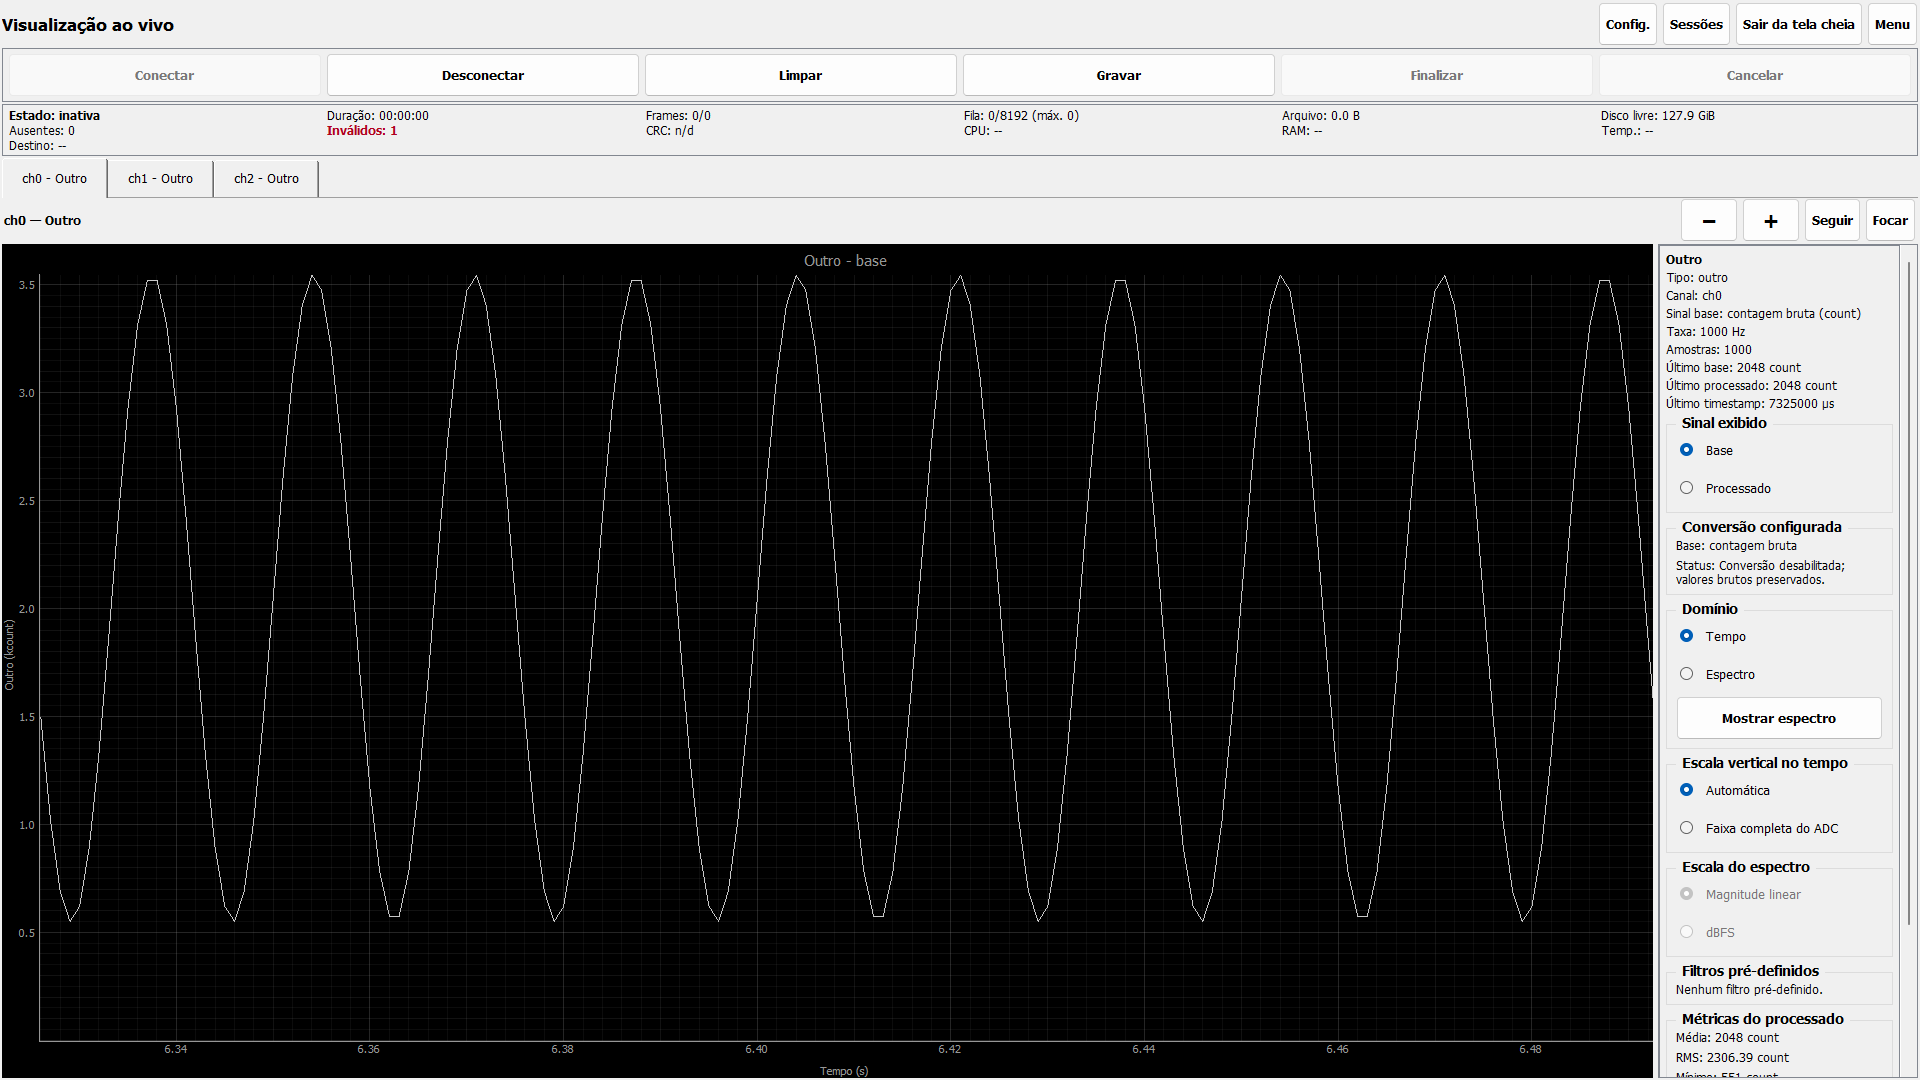
\includegraphics[width=\textwidth]{figuras/print_aquisicao.png} [ph só se der, tira um print da tela do programa funcionando na raspberry e coloca aqui]
    \caption[Interface de visualização ao vivo do software de aquisição]{Interface de visualização ao vivo do software de aquisição, com a apresentação de um sinal periódico no domínio do tempo e os controles de configuração, processamento e visualização do canal.}
    \label{fig:interface_aquisicao}
\end{figure}

A gravação foi realizada em arquivos HDF5 de forma independente do buffer utilizado pela interface. Durante uma sessão ativa, o arquivo recebeu temporariamente a extensão \texttt{.partial.h5}. Após o encerramento correto, o registro foi convertido em um arquivo \texttt{.h5} definitivo.

A estrutura HDF5 preservou separadamente o número sequencial, a marcação temporal em microssegundos e os valores brutos dos canais. Informações como tensão de referência, ganho do amplificador programável, configuração dos canais e filtros selecionados foram mantidas como metadados. A compressão GZIP foi empregada para reduzir o espaço ocupado sem alterar os dados armazenados.

As sessões concluídas puderam ser reabertas pelo próprio programa, verificadas quanto à integridade, visualizadas por intervalos e exportadas integralmente para arquivos CSV. A verificação de integridade utilizou um resumo SHA-256. Nos casos em que uma sessão era interrompida antes da finalização, o programa permitiu recuperar o conteúdo que havia sido confirmado no arquivo até o momento da interrupção.

Para os registros de 30~s realizados com taxa nominal de 1~kS/s por canal, os arquivos HDF5 apresentaram tamanho médio aproximado de 1,8~MB. Os arquivos CSV obtidos após a exportação também apresentaram tamanho médio próximo de 1,8~MB nas sessões consideradas. Embora os tamanhos tenham permanecido próximos nessa configuração, o HDF5 ofereceu uma estrutura mais adequada à escrita incremental, à organização interna dos dados, ao armazenamento de metadados e à recuperação das sessões.

A separação entre visualização, processamento e armazenamento permitiu executar a interface na Raspberry Pi 3 B+ sem condicionar a preservação integral dos dados à frequência de atualização gráfica. A redução da quantidade de pontos exibidos, portanto, não alterou os valores registrados nos arquivos.

% ============================================================================
\subsection{Características físicas e custo do sistema}
\label{subsec:caracteristicas_fisicas_custo}

A configuração final foi constituída pela placa perfurada de aquisição, pelo módulo ADS1256, pela STM32 Black Pill, pela tela TFT auxiliar, pela Raspberry Pi 3 B+, pela tela principal de 7~polegadas, pelos módulos de condicionamento, pela bateria e pelos elementos de alimentação e conexão.

As dimensões externas do conjunto foram de [INSERIR COMPRIMENTO]~cm por [INSERIR LARGURA]~cm por [INSERIR ALTURA]~cm. A massa total, considerando [INDICAR OS COMPONENTES INCLUÍDOS NA PESAGEM], foi de aproximadamente [INSERIR MASSA]~g. [ph se conseguir terminar a montagem dele completo, coloca as características aqui]

A Raspberry Pi utilizou um cartão microSD com capacidade de 64~GB, empregado tanto para o sistema operacional e para o programa quanto para o armazenamento das sessões. Como os arquivos HDF5 e CSV gerados nos registros de 30~s apresentaram tamanho médio próximo de 1,8~MB, o volume ocupado por uma sessão individual representou uma parcela reduzida da capacidade total disponível. A capacidade efetivamente destinada às aquisições, entretanto, foi inferior ao valor nominal do cartão devido ao espaço ocupado pelo sistema operacional, pelo programa e pelos demais arquivos da plataforma.

O custo do sistema foi estimado com base no custo médio de reposição dos componentes. Para essa estimativa, foram considerados preços de componentes novos, iguais ou tecnicamente equivalentes aos utilizados no protótipo, observados entre outubro e dezembro de 2025. O valor atribuído a cada item correspondeu à média dos preços encontrados no período considerado, sem a inclusão dos custos de frete.

A Tabela~\ref{tab:custo_plataforma} apresenta os valores utilizados na estimativa do custo de reposição da plataforma. [ph a gente fala no texto que era baixo custo, essa tabela é pra justificar isso. Caso não tenha ou não ache nescessário, troca isso por algo mais genérico]

\begin{table}[!htbp]
    \centering
    \caption{Custo médio de reposição dos componentes utilizados na plataforma, considerando preços observados entre outubro e dezembro de 2025.}
    \label{tab:custo_plataforma}
    \small
    \begin{tabular}{p{7.0cm} c c}
        \hline
        \textbf{Componente} &
        \textbf{Quantidade} &
        \textbf{Custo médio de reposição} \\
        \hline

        Módulo conversor ADS1256 &
        1 &
        R\$~[INSERIR VALOR] \\

        STM32 Black Pill com STM32F411 &
        1 &
        R\$~[INSERIR VALOR] \\

        Raspberry Pi 3 Model B+ &
        1 &
        R\$~[INSERIR VALOR] \\

        Tela sensível ao toque de 7~polegadas &
        1 &
        R\$~[INSERIR VALOR] \\

        Tela TFT auxiliar de 1,8~polegadas &
        1 &
        R\$~[INSERIR VALOR] \\

        Módulo AD8232 &
        2 &
        R\$~[INSERIR VALOR TOTAL] \\

        Pulse Sensor Amped &
        1 &
        R\$~[INSERIR VALOR] \\

        Bateria e elementos de alimentação &
        1 &
        R\$~[INSERIR VALOR] \\

        Cartão microSD de 64~GB &
        1 &
        R\$~[INSERIR VALOR] \\

        Placa perfurada, cabos, conectores e materiais auxiliares &
        -- &
        R\$~[INSERIR VALOR] \\

        \hline
        \textbf{Custo total médio de reposição} &
        -- &
        \textbf{R\$~[INSERIR VALOR TOTAL]} \\
        \hline
    \end{tabular}
\end{table}

A estimativa considerou apenas os componentes incorporados ao protótipo. Não foram incluídos os instrumentos de bancada utilizados nos ensaios, os custos de desenvolvimento, a mão de obra ou os custos associados à fabricação de uma estrutura mecânica definitiva. Dessa forma, o valor apresentado representa o custo aproximado de reposição do protótipo acadêmico, e não o custo de produção de uma versão comercial.

% ============================================================================
\section{Resultados dos ensaios com sinais conhecidos}
\label{sec:resultados_sinais_conhecidos}

Os ensaios com sinais conhecidos foram realizados para avaliar a capacidade da plataforma de preservar as características temporais e espectrais das formas de onda aplicadas às entradas do ADS1256. Os sinais foram produzidos pelo gerador Politerm POL-40 e encaminhados simultaneamente ao sistema desenvolvido e ao osciloscópio BK Precision 2530, utilizado como instrumento de referência. Essa configuração permitiu comparar as frequências, amplitudes e formas de onda obtidas pelas duas cadeias de medição sob as mesmas condições de geração.

Os registros foram analisados nos domínios do tempo e da frequência. No domínio do tempo, foram consideradas medidas como valores mínimo e máximo, amplitude pico a pico, componente contínua, valor eficaz, frequência estimada e ajuste da forma de onda. No domínio da frequência, foram avaliadas a localização e a amplitude da componente fundamental, as componentes espúrias, a faixa dinâmica livre de espúrios e a relação entre as frequências aplicadas e o limite de Nyquist da aquisição.

As análises foram realizadas sobre os dados convertidos para tensão, considerando a resolução de 24~bits do ADS1256, tensão de referência de 2,5~V e ganho unitário do amplificador de ganho programável. Quando os registros apresentaram descontinuidades temporais, os cálculos espectrais foram realizados sobre os segmentos contíguos identificados, evitando a introdução de transições artificiais entre trechos separados da aquisição.

% ----------------------------------------------------------------------------
\subsection{Sinais senoidais de 100 Hz e 450 Hz}
\label{subsec:senoides_alta_frequencia}

Nesta configuração, o gerador foi ajustado para produzir duas senoides com frequências nominais de 100~Hz e 450~Hz, amplitude configurada em 2~V e componente contínua nula. Os sinais foram adquiridos com taxa nominal de 1~kS/s por canal. A escolha dessas frequências permitiu comparar uma condição com quantidade relativamente elevada de amostras por período com outra próxima ao limite de Nyquist da aquisição.

A frequência média calculada a partir dos intervalos regulares entre quadros foi de aproximadamente 1000,14~Hz, resultando em uma frequência de Nyquist de 500,07~Hz. Dessa forma, a senoide de 100~Hz correspondeu a aproximadamente 20,00\% do limite de Nyquist, enquanto a senoide de 450~Hz correspondeu a aproximadamente 89,98\% desse limite.

\subsubsection{Resultados no domínio do tempo}
\label{subsubsec:senoides_altas_tempo}

Para a senoide de 100~Hz, foram observados valores mínimo e máximo de $-1,0272$~V e $1,0316$~V, respectivamente, resultando em uma amplitude pico a pico observada de 2,0588~V. A componente contínua foi de aproximadamente 7,94~mV, enquanto o valor eficaz total foi de 0,7272~V. O ajuste senoidal forneceu uma amplitude de pico de 1,0284~V, correspondente a 2,0569~V de pico a pico, e um valor eficaz fundamental de 0,7272~V.

A frequência estimada para esse canal foi de 99,9963~Hz, correspondente a um período de 10,0004~ms. A taxa efetiva de aquisição resultou em aproximadamente 10,00 amostras por período e em um avanço de fase de aproximadamente $35,99^{\circ}$ entre amostras consecutivas. O ajuste senoidal apresentou coeficiente de determinação de 0,99994 e erro quadrático médio normalizado de 0,7733\%, indicando elevada correspondência entre as amostras adquiridas e o modelo senoidal ajustado.

Para a senoide de 450~Hz, os valores mínimo e máximo foram de $-1,0180$~V e $1,0196$~V, resultando em uma amplitude pico a pico observada de 2,0375~V. A componente contínua foi de aproximadamente 9,31~mV e o valor eficaz total foi de 0,7186~V. O ajuste senoidal forneceu amplitude de pico de 1,0154~V, correspondente a 2,0308~V de pico a pico, e valor eficaz fundamental de 0,7180~V.

A frequência estimada para esse sinal foi de 449,9835~Hz, correspondente a um período de 2,2223~ms. Em razão da proximidade com o limite de Nyquist, foram obtidas apenas aproximadamente 2,22 amostras por período, com avanço de fase de $161,97^{\circ}$ entre amostras consecutivas. Apesar da baixa densidade temporal, o ajuste apresentou coeficiente de determinação de 0,99989 e erro quadrático médio normalizado de 1,0407\%.

A Figura~\ref{fig:amostragem_senoides_altas} apresenta as amostras adquiridas e as senoides ajustadas para os dois sinais. No sinal de 100~Hz, os pontos descrevem de forma direta a evolução da senoide ao longo de cada período. No sinal de 450~Hz, a quantidade reduzida de pontos por ciclo dificulta o reconhecimento visual da forma de onda quando são consideradas apenas as amostras isoladas, embora o ajuste demonstre a correspondência dessas amostras com uma componente senoidal de frequência próxima à configurada.

\begin{figure}[!htbp]
    \centering
    \begin{minipage}[t]{0.9\textwidth}
        \centering
        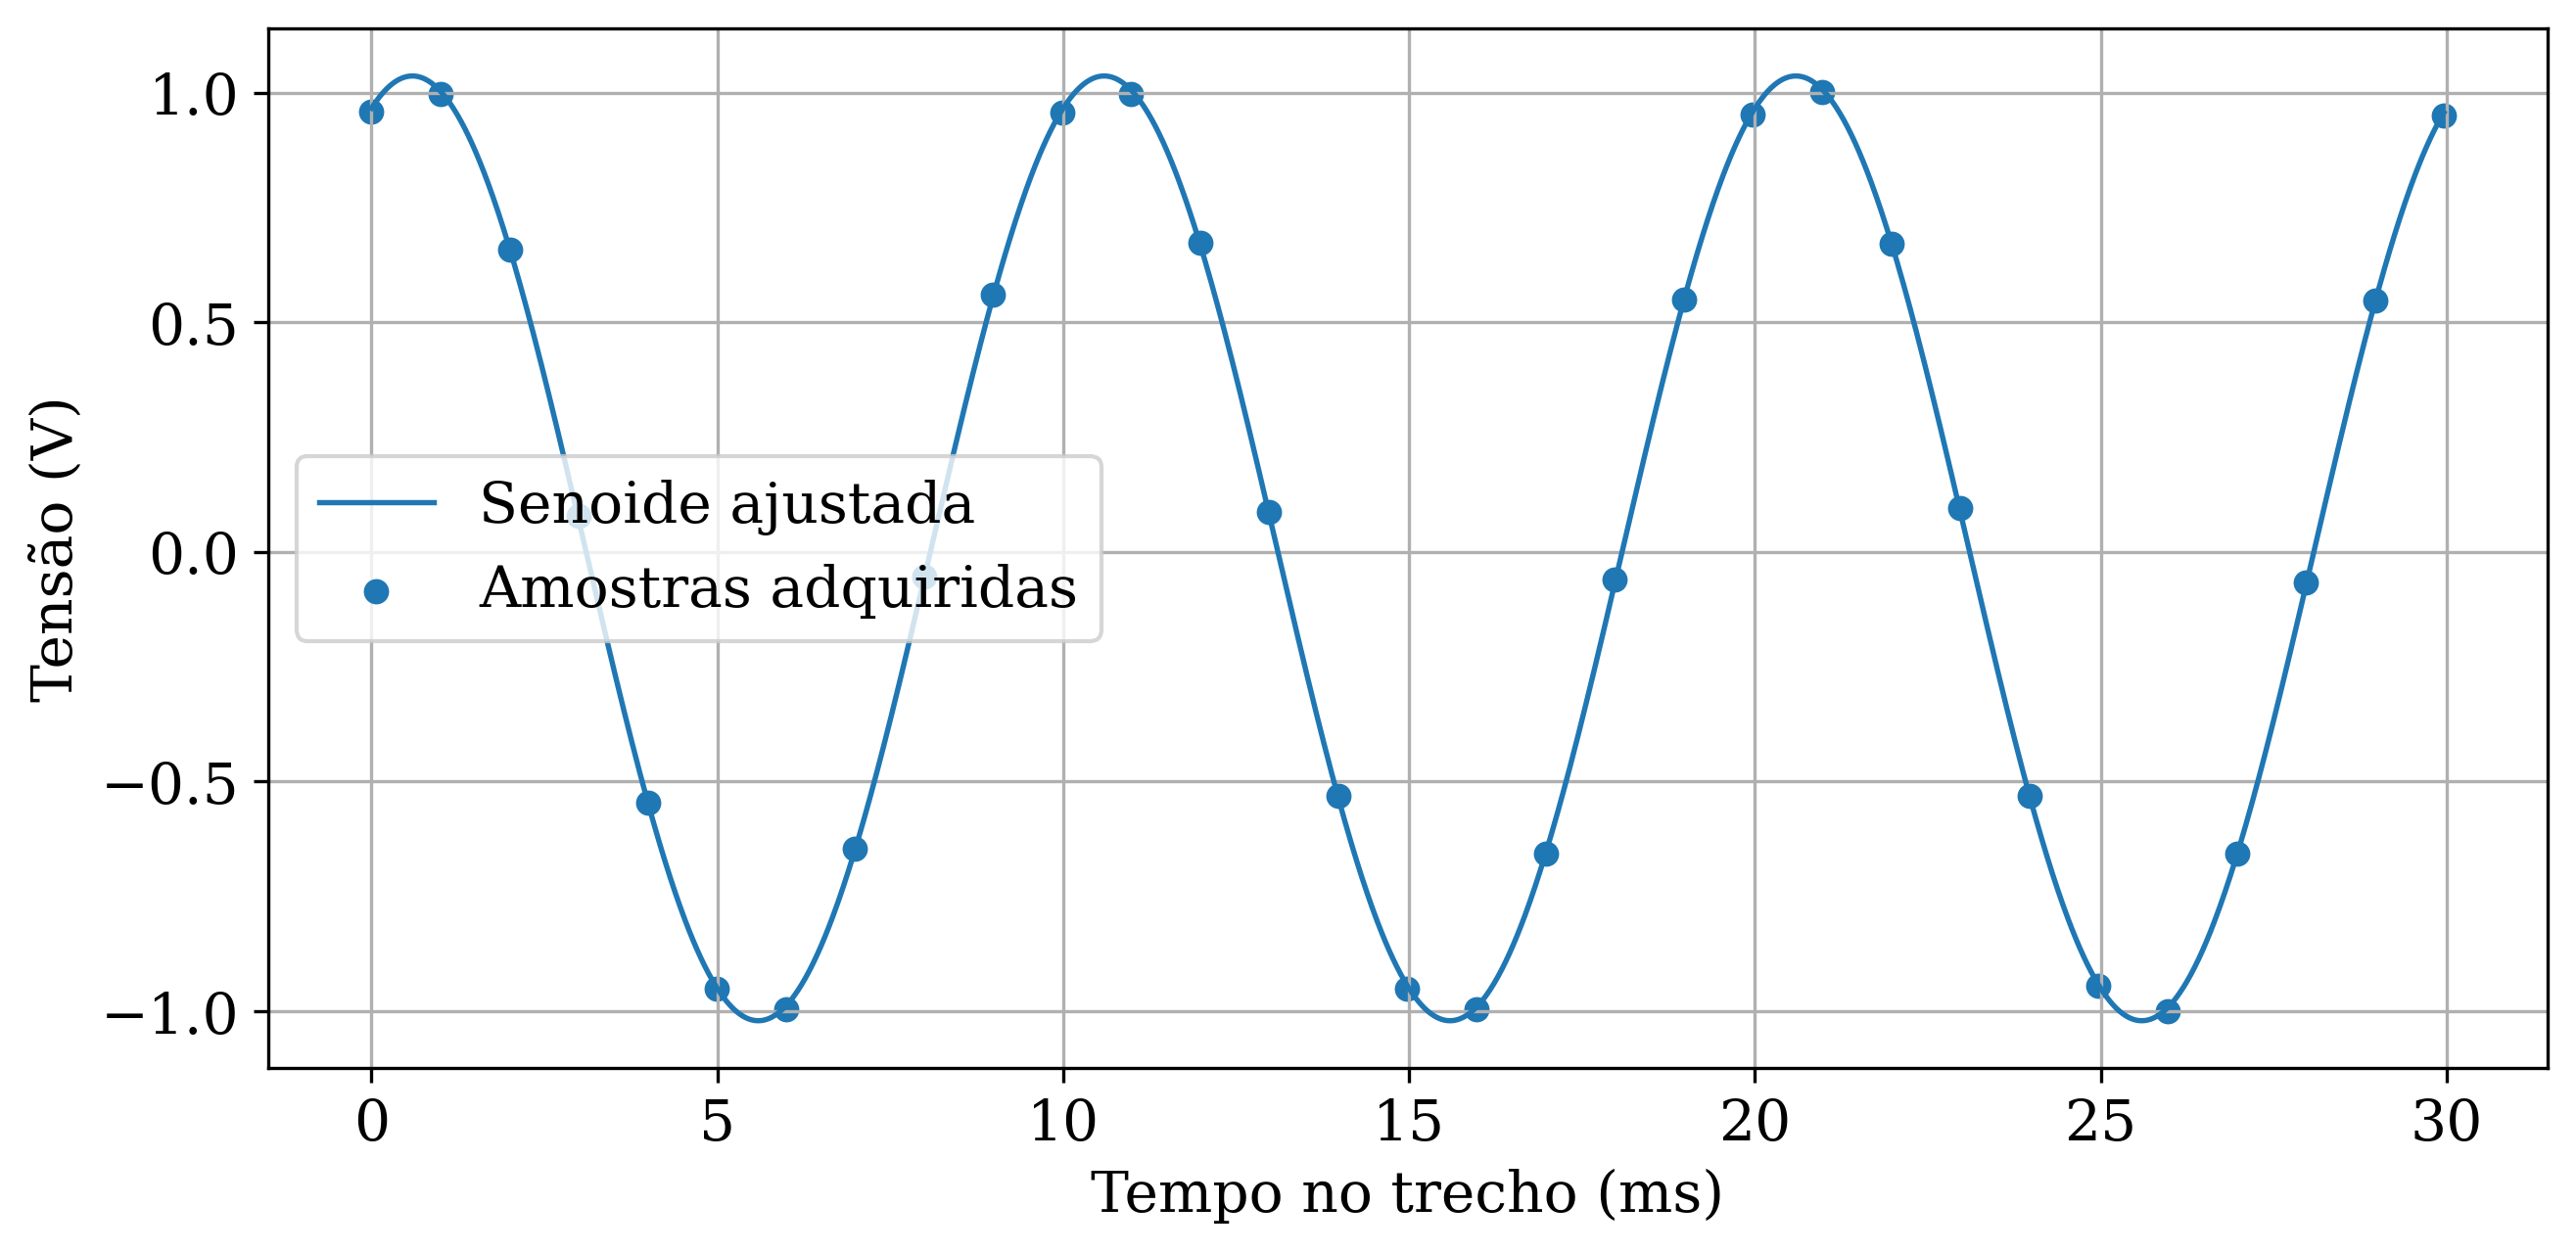
\includegraphics[width=\textwidth]{figuras/figura_amostragem_100Hz.png}
        \small (a) Sinal senoidal de 100~Hz.
    \end{minipage}

    \begin{minipage}[t]{0.9\textwidth}
        \centering
        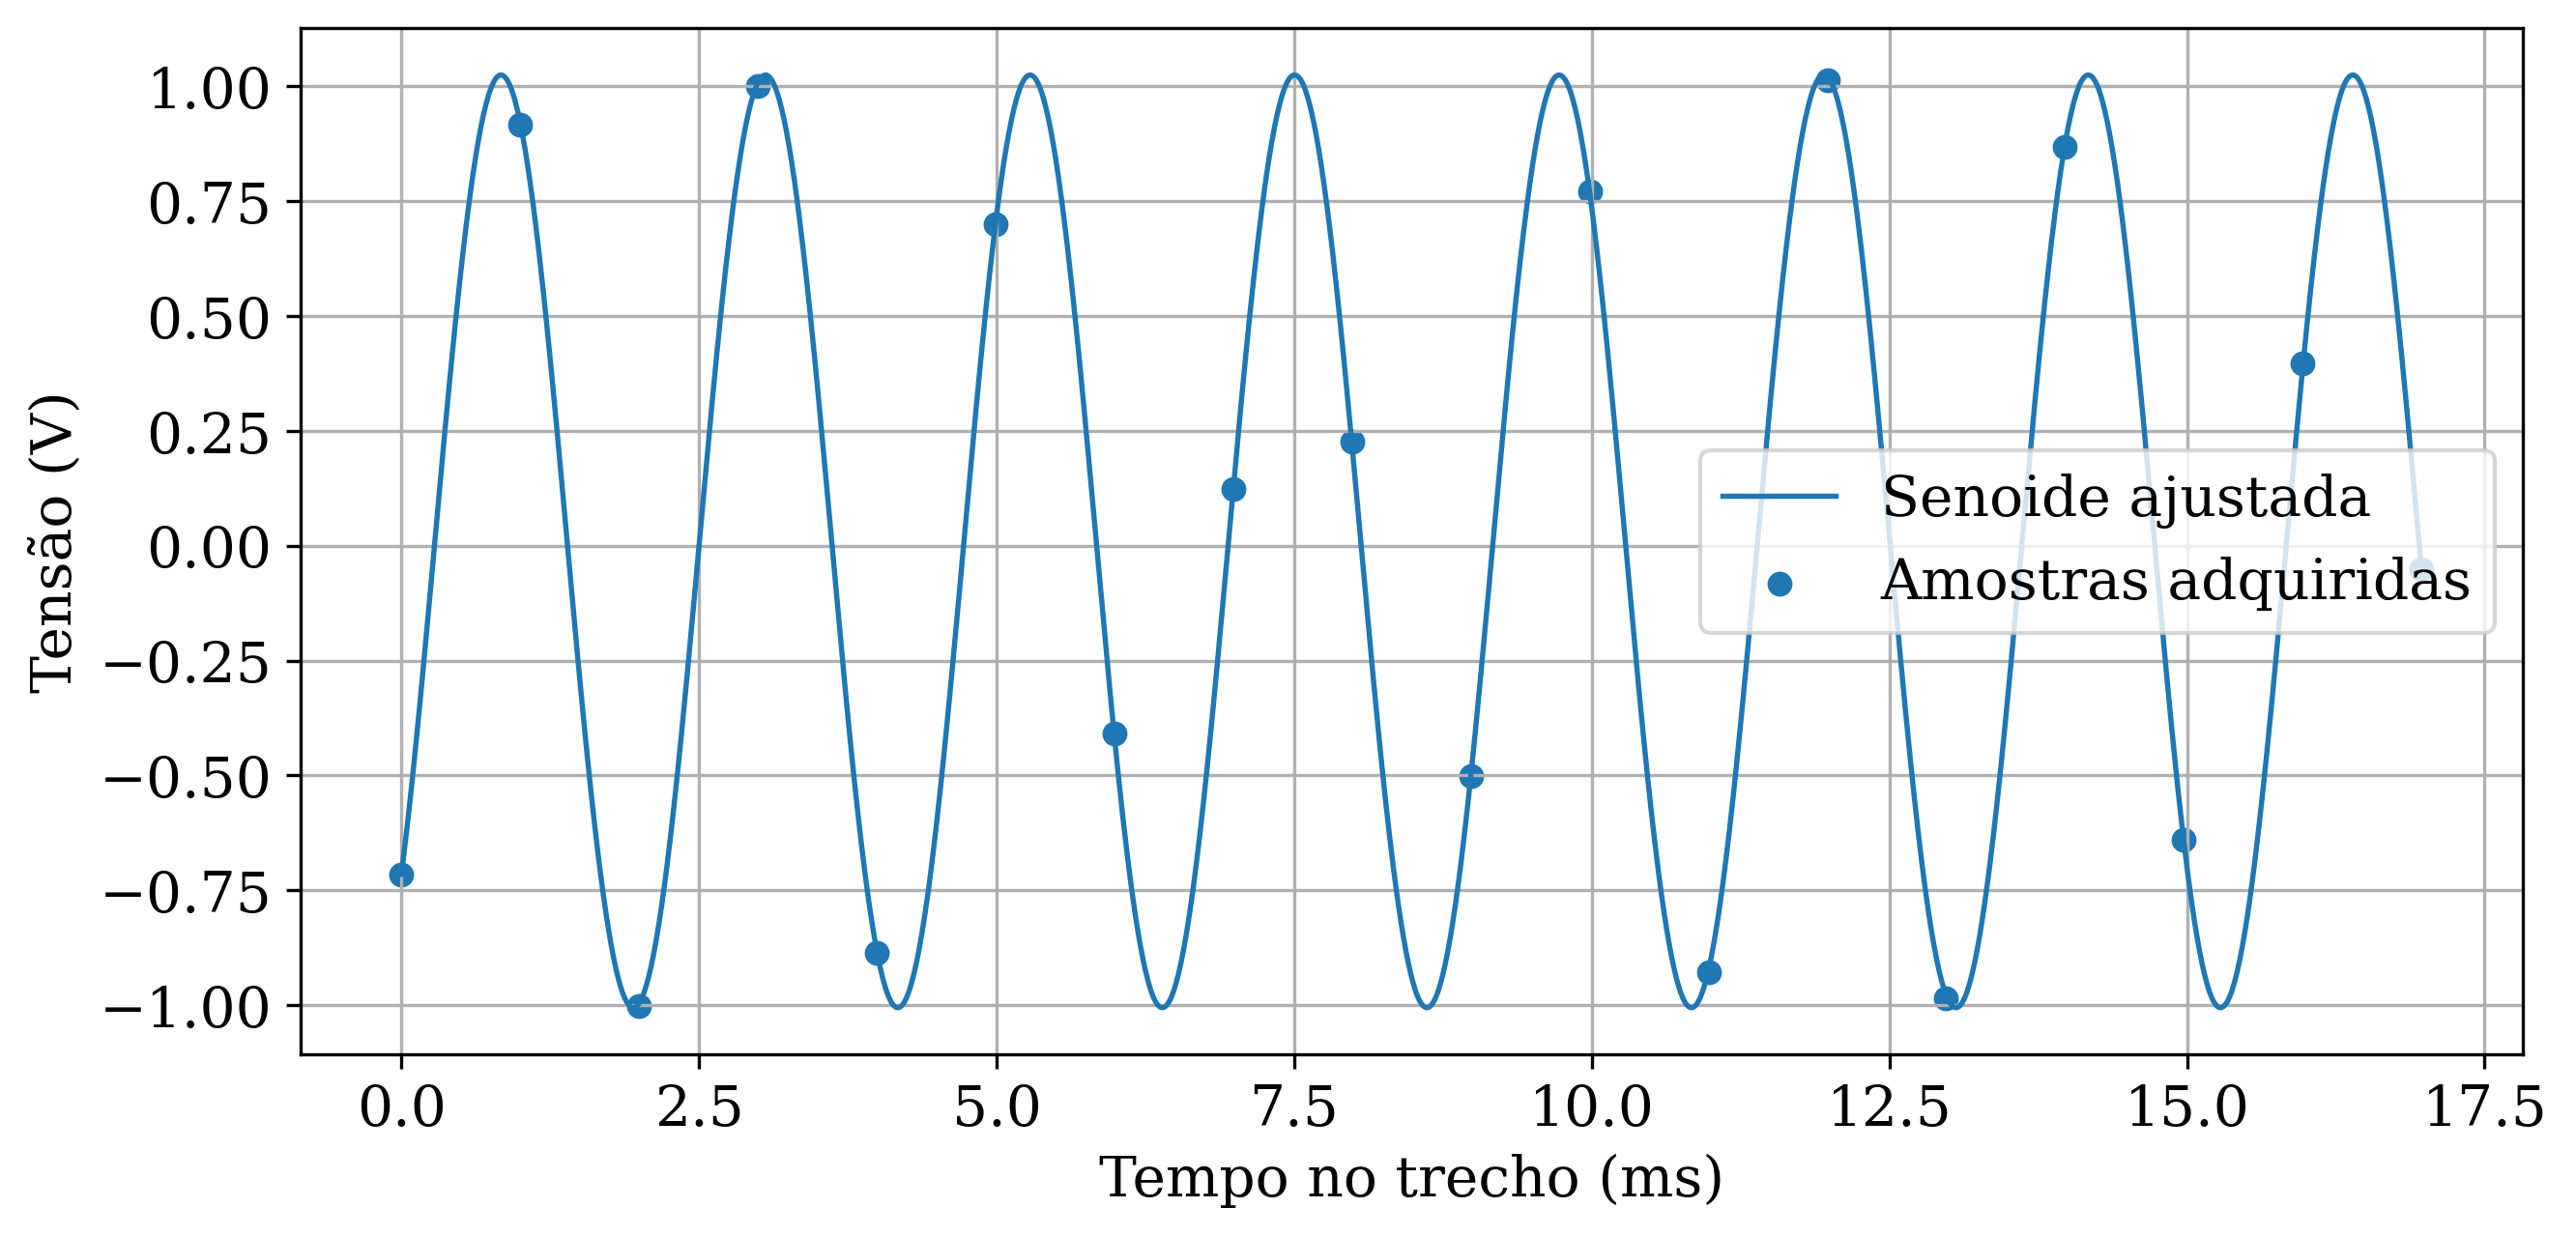
\includegraphics[width=\textwidth]{figuras/figura_amostragem_450Hz.png}
        \small (b) Sinal senoidal de 450~Hz.
    \end{minipage}

    \caption[Amostragem de senoides de 100 e 450~Hz]{
        Comparação entre as amostras adquiridas, representadas pelos marcadores, e as senoides ajustadas, representadas pelas linhas contínuas, para sinais de (a) 100~Hz e (b) 450~Hz, ambos amostrados à taxa de 1~kHz. Nessa taxa, o sinal de 100~Hz apresenta 10 amostras por período, enquanto o sinal de 450~Hz apresenta aproximadamente 2,22 amostras por período, evidenciando
        a redução da resolução temporal à medida que a frequência do sinal se aproxima da frequência de Nyquist, igual a 500~Hz.
    }
    \label{fig:amostragem_senoides_altas}
\end{figure}

A comparação direta entre os sinais no mesmo intervalo temporal é apresentada na Figura~\ref{fig:comparacao_temporal_senoides_altas}. A linha que conecta as amostras constitui apenas um recurso de visualização e não representa a reconstrução contínua dos sinais. Essa distinção é especialmente importante para a senoide de 450~Hz, cuja variação de fase entre amostras consecutivas se aproxima de $180^{\circ}$.

\begin{figure}[!htbp]
    \centering
    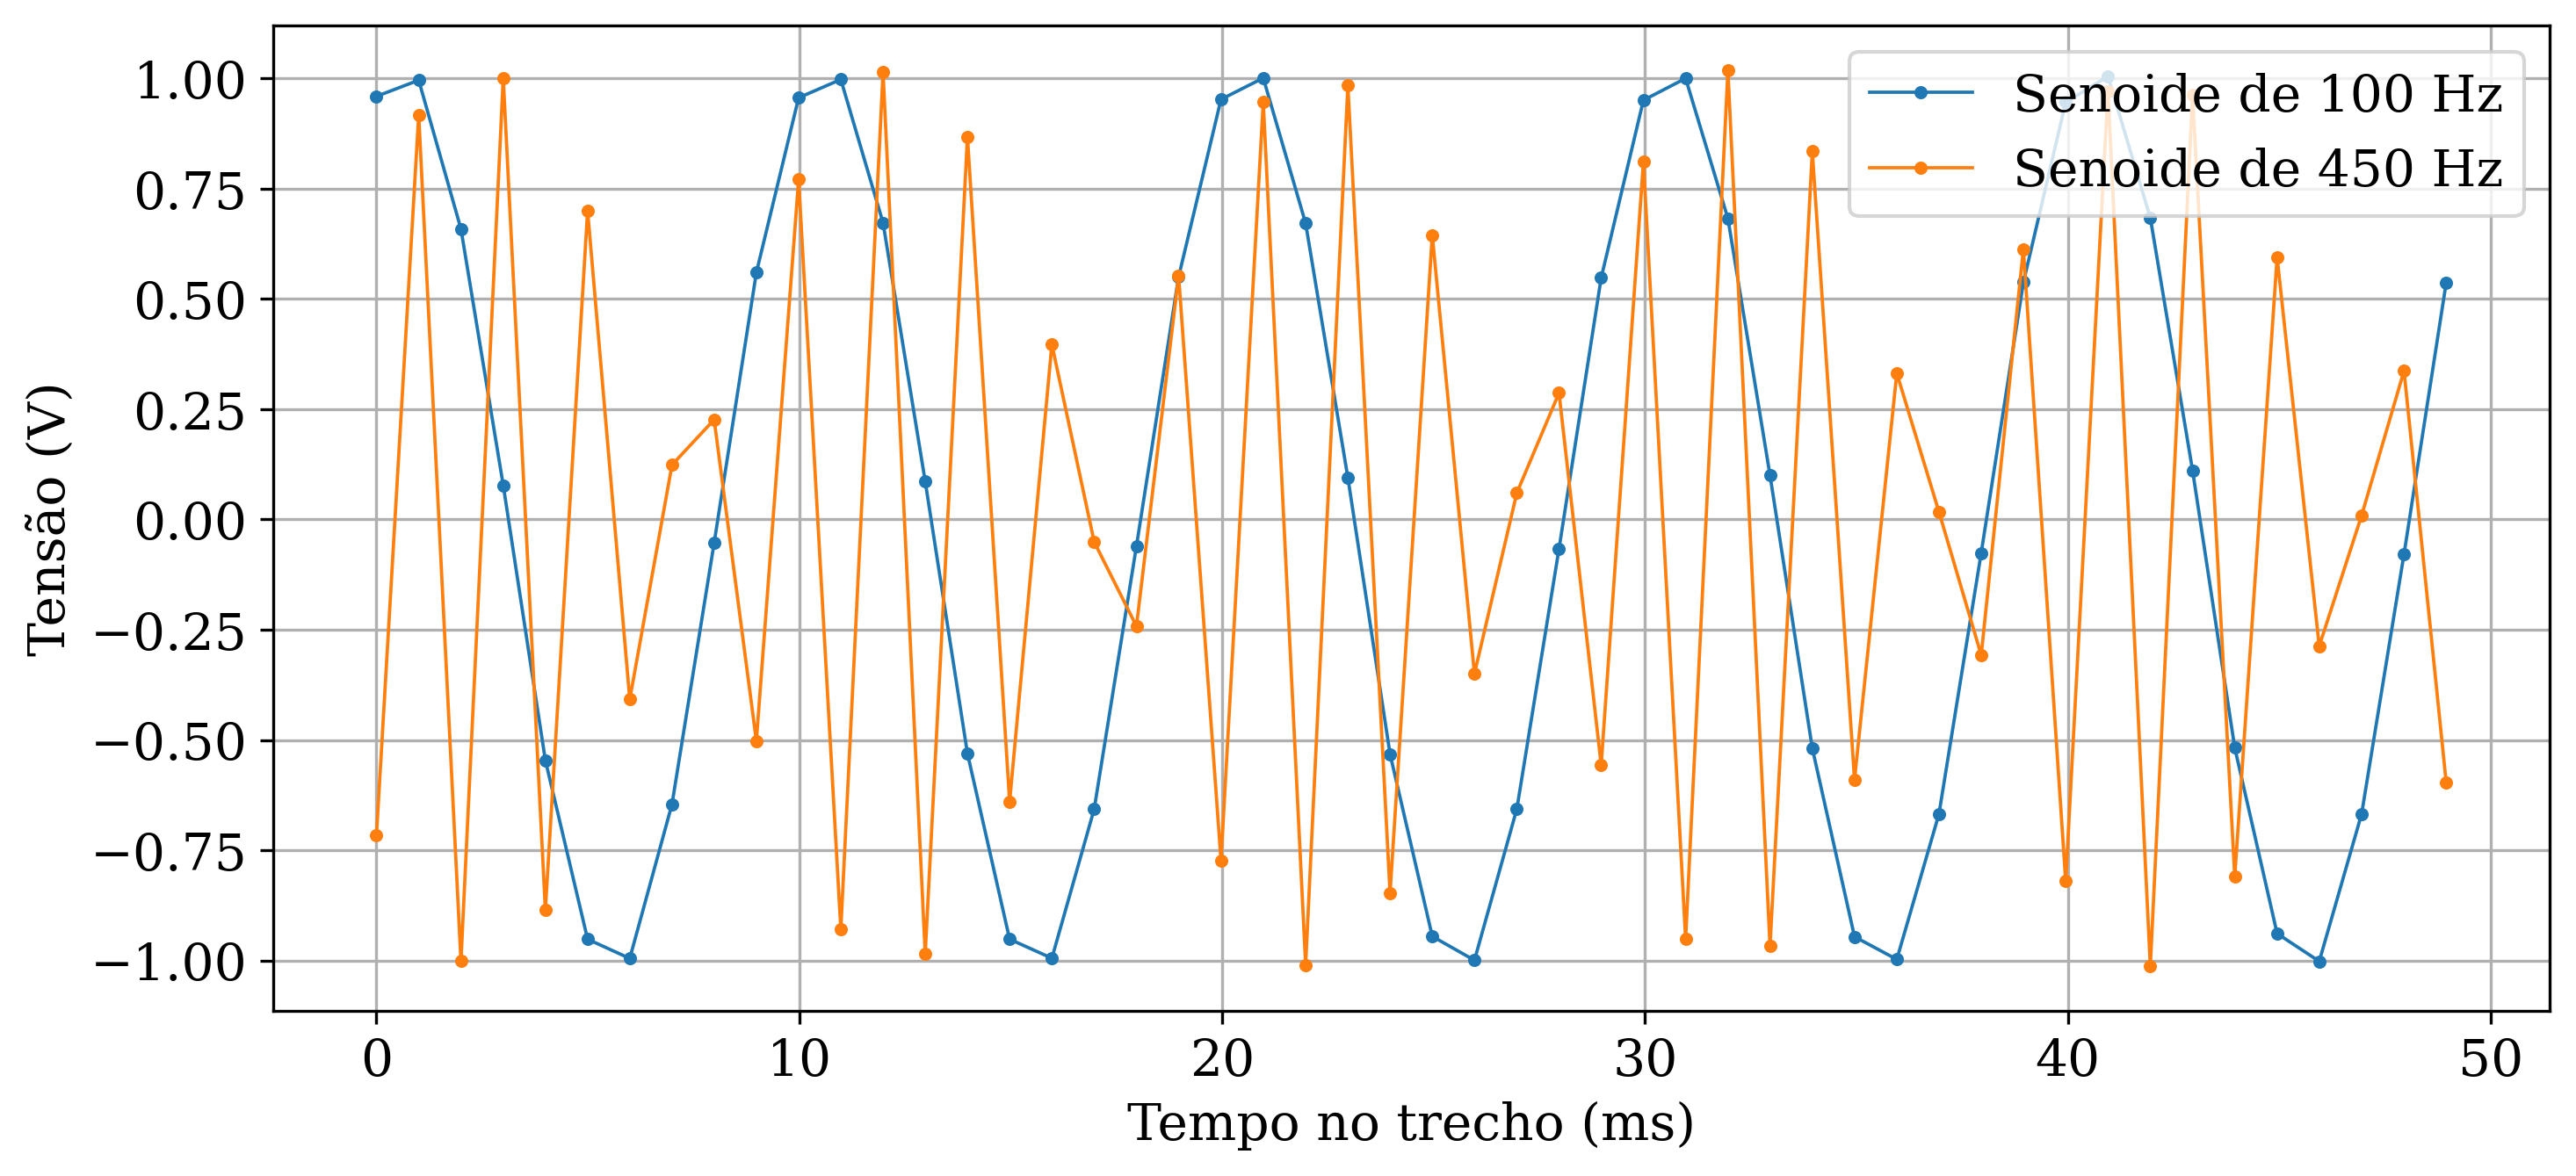
\includegraphics[width=\textwidth]{figuras/figura_tempo_comparativo_100Hz_450Hz.png}
    \caption[Comparação temporal de senoides de 100 e 450~Hz]{
        Comparação, em um trecho de 50~ms, entre as amostras de sinais senoidais de 100~Hz e 450~Hz adquiridas à taxa de amostragem de 1~kHz. Os marcadores representam as amostras consecutivas e as linhas apenas auxiliam na visualização de sua evolução temporal. O sinal de 100~Hz apresenta 10 amostras por período, resultando em uma representação temporal bem definida, enquanto o sinal de 450~Hz apresenta aproximadamente 2,22 amostras por período, evidenciando a representação mais esparsa de sinais com frequência próxima à frequência de Nyquist, igual a 500~Hz.
    }
    \label{fig:comparacao_temporal_senoides_altas}
\end{figure}

A Tabela~\ref{tab:metricas_tempo_senoides_altas} reúne as principais métricas temporais obtidas para os dois canais.

\begin{table}[!htbp]
    \centering
    \caption{Métricas no domínio do tempo para as senoides de 100~Hz e 450~Hz.}
    \label{tab:metricas_tempo_senoides_altas}
    \small
    \begin{tabular}{l c c c}
        \hline
        \textbf{Métrica} &
        \textbf{Unidade} &
        \textbf{100~Hz} &
        \textbf{450~Hz} \\
        \hline
        $V_{\mathrm{pp}}$ observado & V   & 2,0588   & 2,0375   \\
        $V_{\mathrm{pp}}$ ajustado  & V   & 2,0569   & 2,0308   \\
        RMS                         & V   & 0,7272   & 0,7186   \\
        Componente CC               & mV  & 7,94     & 9,31     \\
        Frequência                  & Hz  & 99,9963  & 449,9835 \\
        Período                     & ms  & 10,0004  & 2,2223   \\
        Amostras/período            & --  & 10,00    & 2,22     \\
        $R^2$                       & --  & 0,99994  & 0,99989  \\
        NRMSE                       & \%  & 0,7733   & 1,0407   \\
        \hline
    \end{tabular}
\end{table}


As capturas do osciloscópio utilizadas como referência são apresentadas nas Figuras~\ref{fig:osciloscopio_senoides_altas} e \ref{fig:osciloscopio_medidas_senoides_altas}. Na medição detalhada, o osciloscópio indicou frequência de 100,24~Hz para o primeiro canal e de 450,22~Hz para o segundo. Para ambos os sinais, foi registrada amplitude pico a pico de 2,24~V e valor eficaz de 706,54~mV.

\begin{figure}[!htbp]
    \centering
    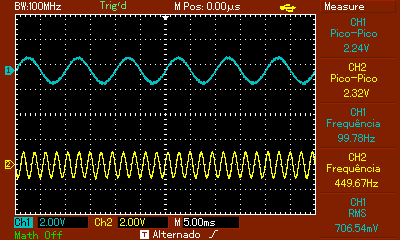
\includegraphics[width=0.9\textwidth]
    {figuras/osciloscopio_senoides_100Hz_450Hz.png}
    \caption[Senoides de 100 e 450~Hz no osciloscópio]{
        Visualização simultânea, no osciloscópio, dos sinais senoidais
        aplicados aos canais CH1 e CH2. O canal CH1, representado em ciano,
        corresponde ao sinal de aproximadamente 100~Hz, enquanto o canal
        CH2, representado em amarelo, corresponde ao sinal de aproximadamente
        450~Hz. As medições apresentadas na tela indicam frequências de
        99,78~Hz e 449,67~Hz, respectivamente, e tensão de pico a pico de
        2,24~V para ambos os sinais. A base de tempo de 5~ms por divisão
        permite observar aproximadamente cinco períodos do sinal de 100~Hz
        e 22,5 períodos do sinal de 450~Hz no intervalo exibido.
    }
    \label{fig:osciloscopio_senoides_altas}
\end{figure}

\begin{figure}[!htbp]
    \centering

    \begin{minipage}[t]{0.9\textwidth}
        \centering
        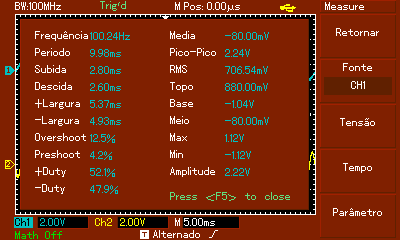
\includegraphics[width=\textwidth]
        {figuras/osciloscopio_medidas_100Hz.png}
        \small (a) Medições automáticas do sinal de aproximadamente 100~Hz
        no canal CH1.
    \end{minipage}

    \medskip

    \begin{minipage}[t]{0.9\textwidth}
        \centering
        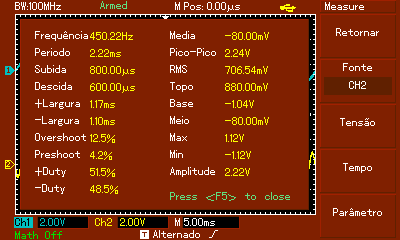
\includegraphics[width=\textwidth]
        {figuras/osciloscopio_medidas_450Hz.png}
        \small (b) Medições automáticas do sinal de aproximadamente 450~Hz
        no canal CH2.
    \end{minipage}

    \caption[Medições das senoides de 100 e 450~Hz]{
        Medições automáticas realizadas pelo osciloscópio para os sinais
        senoidais de (a) aproximadamente 100~Hz, aplicado ao canal CH1, e
        (b) aproximadamente 450~Hz, aplicado ao canal CH2. Para o primeiro
        sinal, foram obtidas frequência de 100,24~Hz e período de 9,98~ms;
        para o segundo, frequência de 450,22~Hz e período de 2,22~ms.
        Em ambas as medições, o osciloscópio indicou tensão de pico a pico
        de 2,24~V, tensão eficaz de aproximadamente 706,54~mV e amplitude
        total de 2,22~V.
    }
    \label{fig:osciloscopio_medidas_senoides_altas}
\end{figure}

Em relação aos valores nominais configurados no gerador, os erros de frequência do sistema foram de $-0,00365$\% para o sinal de 100~Hz e de $-0,00366$\% para o sinal de 450~Hz. Quando comparadas às medições detalhadas do osciloscópio, as diferenças foram de $-0,2431$\% e $-0,0525$\%, respectivamente.

As amplitudes pico a pico fundamentais estimadas pelo sistema ficaram 2,84\% acima do valor nominal de 2~V para o sinal de 100~Hz e 1,54\% acima para o sinal de 450~Hz. Em relação aos 2,24~V de pico a pico indicados pelo osciloscópio, os valores obtidos pelo sistema foram 8,18\% e 9,34\% menores. Os valores eficazes registrados pelo sistema ficaram 2,92\% acima da medição do osciloscópio para 100~Hz e 1,71\% acima para 450~Hz.

A diferença entre as comparações de amplitude pico a pico e de valor eficaz indica influência do método de medição empregado. A amplitude pico a pico do osciloscópio foi calculada a partir dos valores extremos observados, que podem incorporar ruído e pequenas variações locais, enquanto a amplitude fundamental do sistema foi obtida pelo ajuste da componente senoidal. O valor eficaz, por sua vez, representa o comportamento global das amostras ao longo do registro e apresentou diferença inferior à observada na comparação dos extremos.

\subsubsection{Resultados no domínio da frequência}
\label{subsubsec:senoides_altas_frequencia}

A análise espectral identificou componentes fundamentais em 99,9963~Hz e 449,9835~Hz. Os erros absolutos em relação às frequências configuradas foram de $-0,0037$~Hz e $-0,0165$~Hz, correspondendo a erros relativos próximos de $-0,00365$\% nos dois canais.

As amplitudes espectrais de pico foram de 1,0284~V para a componente de 100~Hz e de 1,0154~V para a componente de 450~Hz. Esses valores correspondem a amplitudes pico a pico fundamentais de 2,0569~V e 2,0308~V, respectivamente. A Figura~\ref{fig:espectros_senoides_altas} apresenta os espectros em escala linear e em dBc.

\begin{figure}[!htbp]
    \centering

    \begin{minipage}[t]{0.9\textwidth}
        \centering
        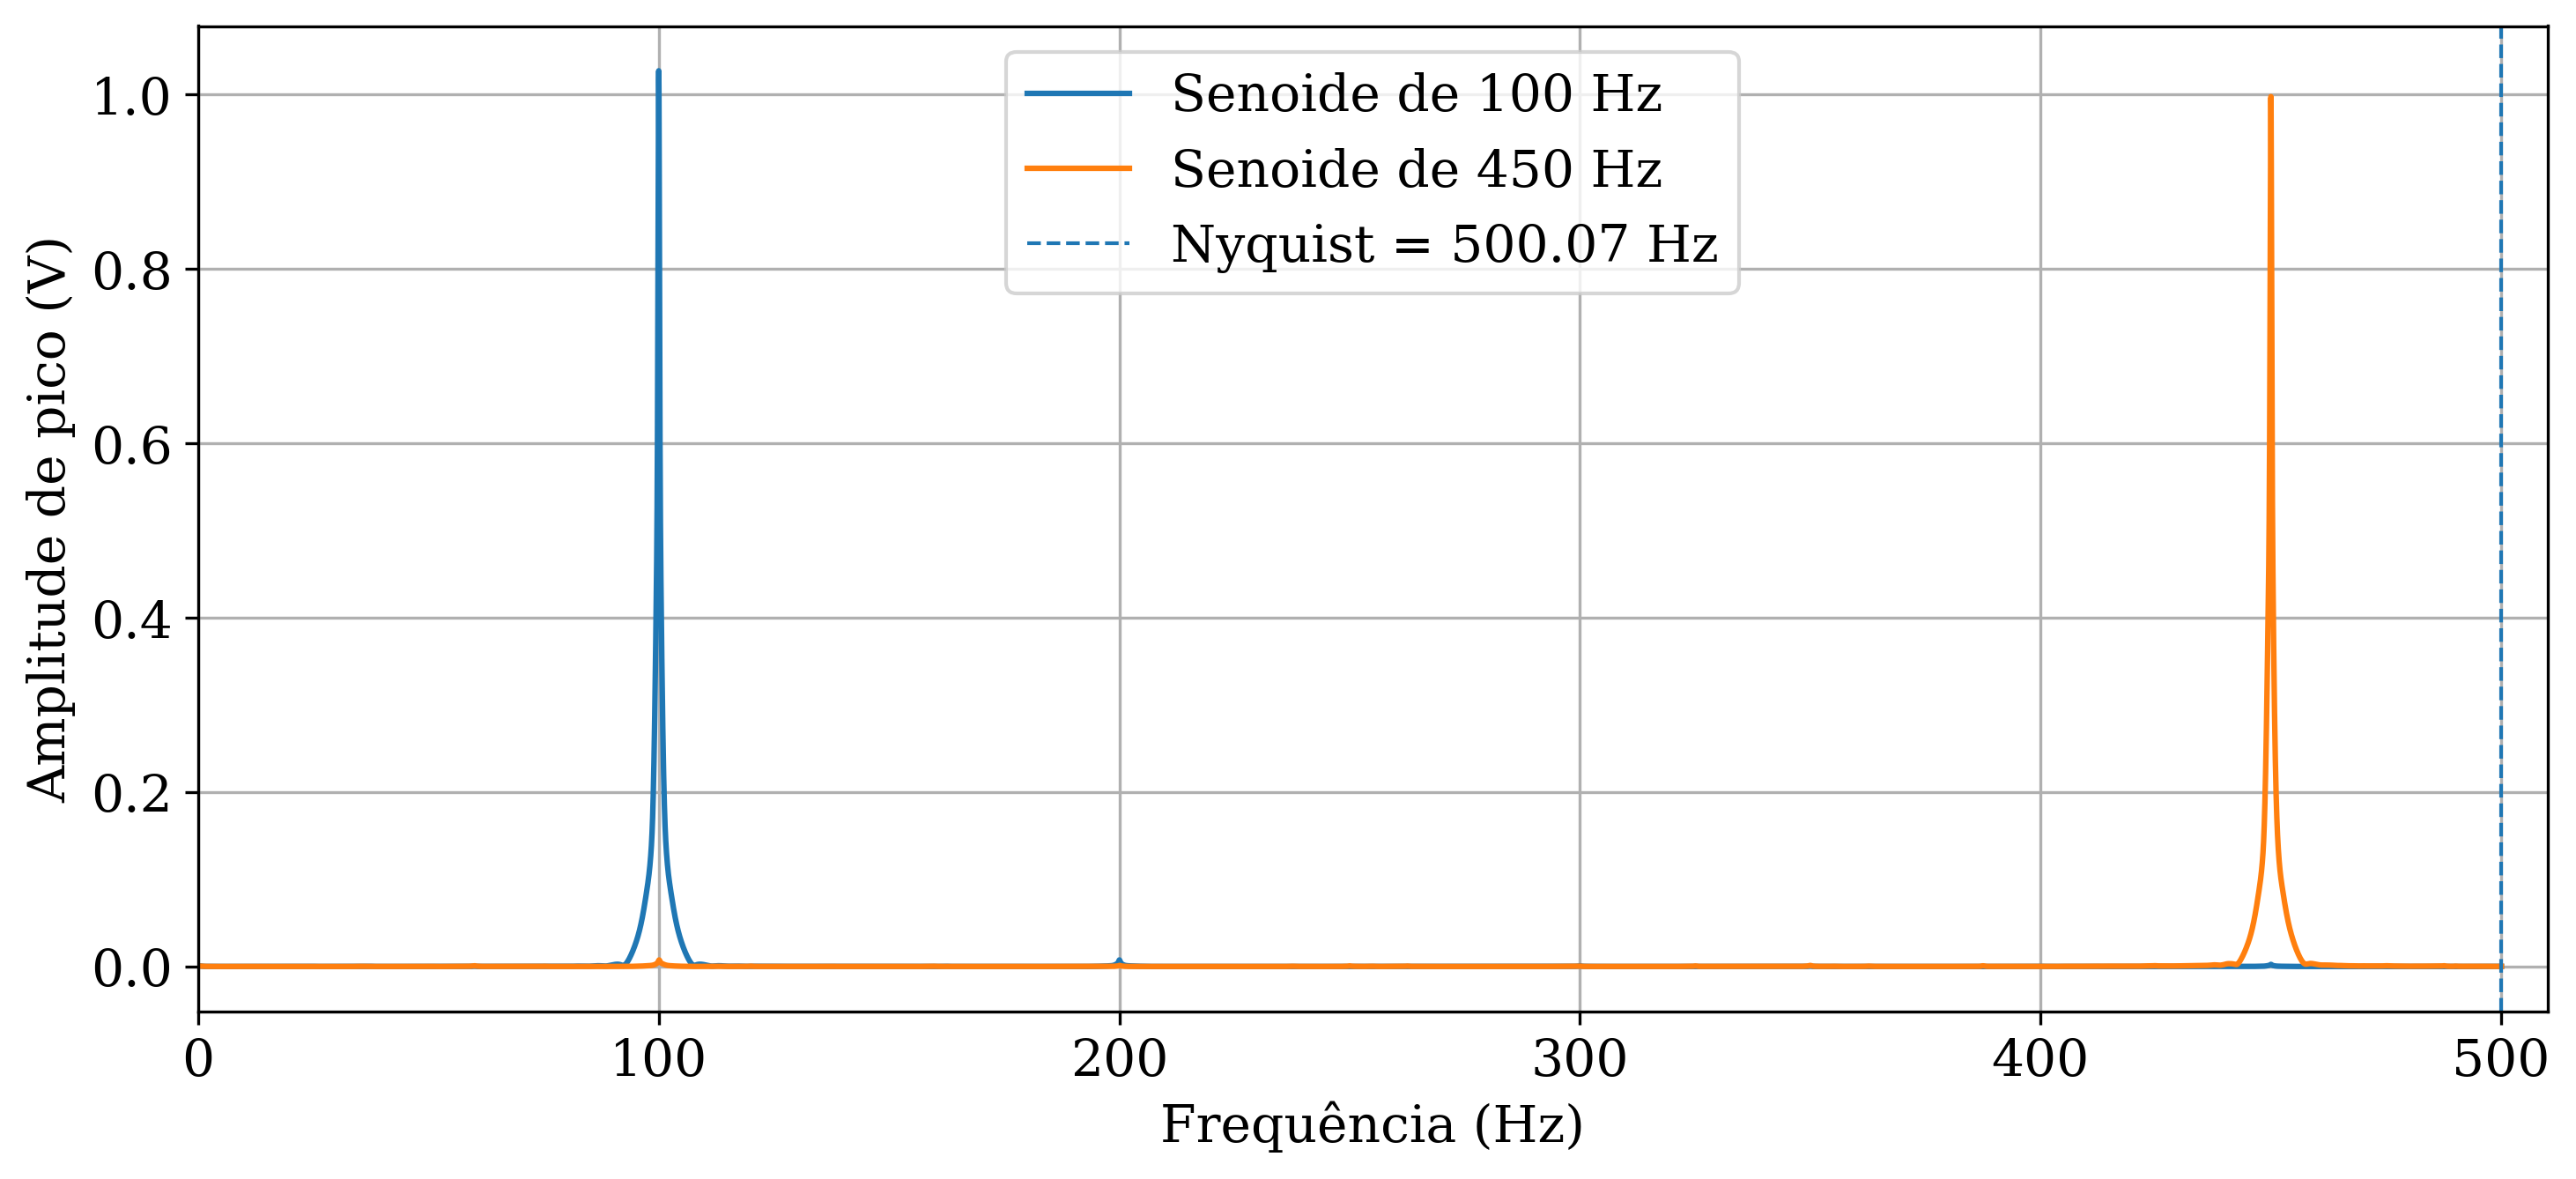
\includegraphics[width=\textwidth]
        {figuras/figura_espectro_linear_100Hz_450Hz.png}
        \small (a) Espectros em amplitude de pico, na escala linear.
    \end{minipage}

    \medskip

    \begin{minipage}[t]{0.9\textwidth}
        \centering
        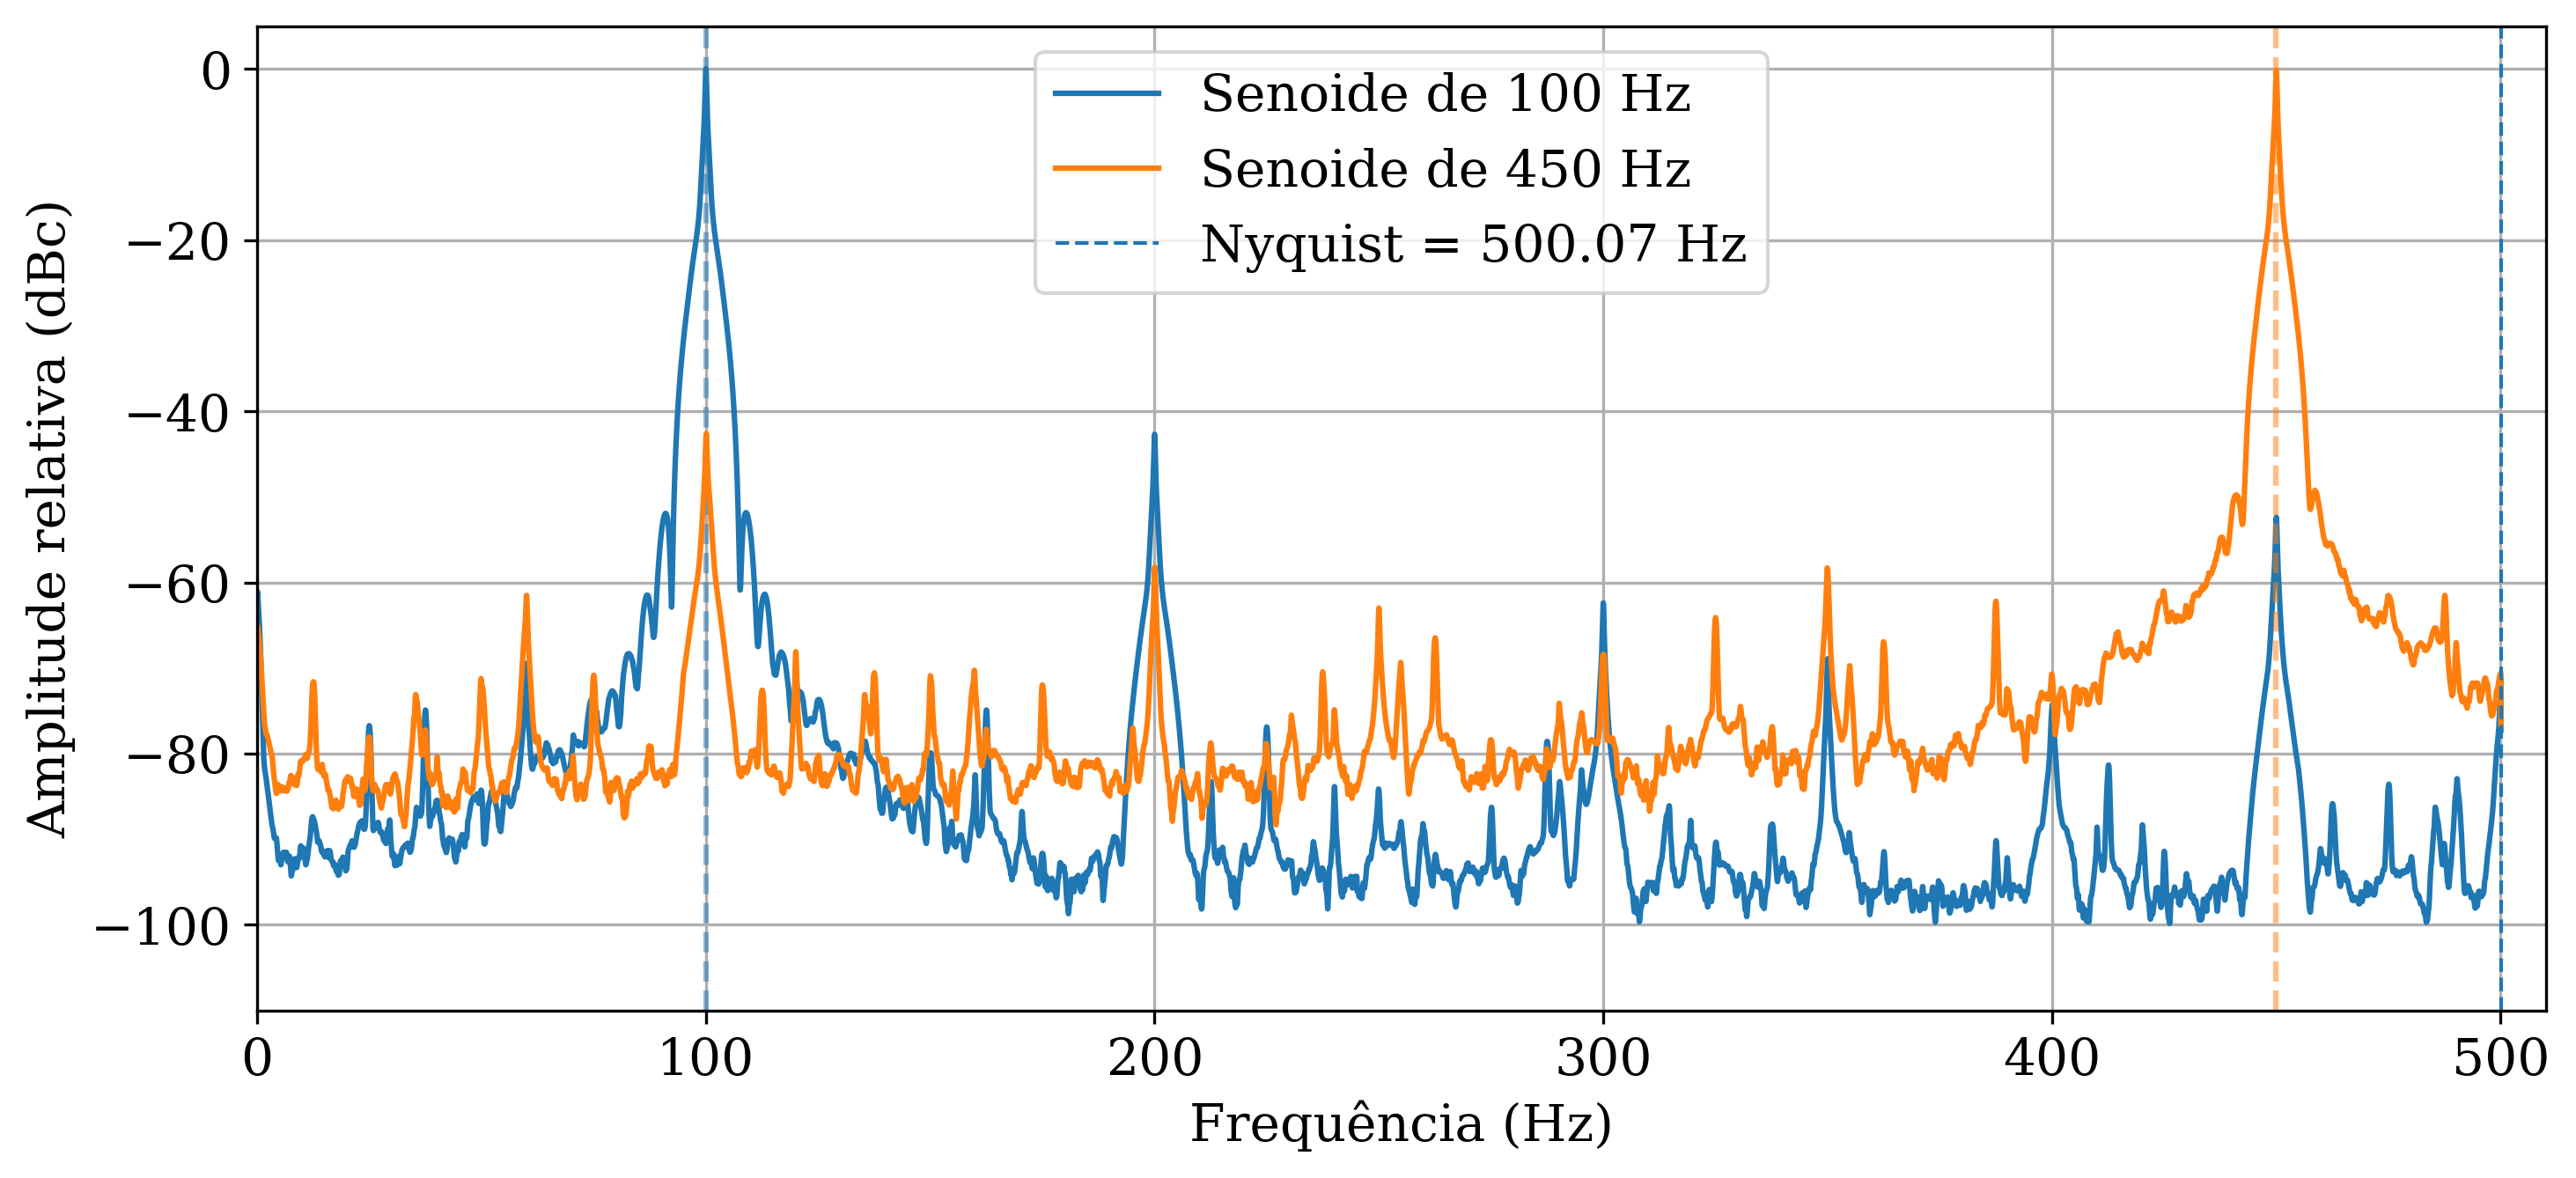
\includegraphics[width=\textwidth]
        {figuras/figura_espectro_dbc_100Hz_450Hz.png}
        \small (b) Espectros normalizados em relação às respectivas
        componentes fundamentais, em dBc.
    \end{minipage}

    \caption[Espectros das senoides de 100 e 450~Hz]{
        Espectros de frequência dos sinais senoidais de 100~Hz e 450~Hz
        adquiridos com frequência de amostragem de aproximadamente
        1~kHz. Em (a), a amplitude espectral é apresentada em escala
        linear, com picos principais próximos de 100~Hz e 450~Hz e
        amplitudes de pico próximas de 1~V. Em (b), cada espectro é
        normalizado em relação à sua respectiva componente fundamental,
        definida como 0~dBc, permitindo visualizar o piso de ruído e as
        demais componentes espectrais. A linha vertical tracejada em
        500,07~Hz indica a frequência de Nyquist; assim, a componente de
        450~Hz encontra-se próxima ao limite superior da faixa de
        frequências representável sem ambiguidade.
    }
    \label{fig:espectros_senoides_altas}
\end{figure}

Para a senoide de 100~Hz, a maior componente espúria foi identificada em 200,0093~Hz, com amplitude de pico de 7,38~mV e nível relativo de $-42,89$~dBc. Essa componente corresponde aproximadamente ao segundo harmônico da frequência fundamental. A componente observada nas proximidades de 450~Hz apresentou amplitude de 2,49~mV e nível relativo de $-52,33$~dBc.

Para a senoide de 450~Hz, a maior componente espúria foi identificada em 100,0962~Hz, com amplitude de pico de 7,94~mV e nível relativo de $-42,13$~dBc. A posição dessa componente é compatível com o dobramento espectral esperado para o segundo harmônico do sinal de 450~Hz. Como esse harmônico estaria localizado próximo de 900~Hz, acima da frequência de Nyquist, sua frequência rebatida para a primeira zona de Nyquist seria próxima de 100,17~Hz.

As relações entre a componente fundamental e a maior componente espúria, expressas pela faixa dinâmica livre de espúrios, foram de 42,89~dB para a senoide de 100~Hz e de 42,13~dB para a senoide de 450~Hz. A interferência próxima de 60~Hz foi observada em níveis de aproximadamente $-70,46$~dBc no canal de 100~Hz e $-60,69$~dBc no canal de 450~Hz.

A Tabela~\ref{tab:metricas_frequencia_senoides_altas} sintetiza os principais resultados espectrais.

\begin{table}[!htbp]
    \centering
    \caption{Métricas no domínio da frequência para as senoides de 100~Hz e 450~Hz.}
    \label{tab:metricas_frequencia_senoides_altas}
    \small
    \begin{tabular}{l c c}
        \hline
        \textbf{Métrica} &
        \textbf{100~Hz} &
        \textbf{450~Hz} \\
        \hline
        Fundamental (Hz)          & 99,9963  & 449,9835 \\
        Erro absoluto (Hz)        & $-0,0037$ & $-0,0165$ \\
        Erro relativo (\%)        & $-0,00365$ & $-0,00366$ \\
        Amplitude de pico (V)     & 1,0284   & 1,0154 \\
        Maior espúria (Hz)        & 200,0093 & 100,0962 \\
        Amplitude da espúria (mV) & 7,38     & 7,94 \\
        SFDR (dB)                 & 42,89    & 42,13 \\
        \hline
    \end{tabular}
\end{table}

A componente fundamental de 450~Hz permaneceu aproximadamente 50,09~Hz abaixo da frequência de Nyquist e foi identificada sem rebatimento para uma frequência inferior. Portanto, o fenômeno de aliasing observado nas proximidades de 100~Hz está associado principalmente às componentes harmônicas acima do limite de Nyquist, e não à componente fundamental de 450~Hz.

\subsubsection{Discussão dos resultados}
\label{subsubsec:discussao_senoides_altas}

O sinal de 100~Hz foi representado por aproximadamente dez amostras em cada período, permitindo que sua forma senoidal fosse reconhecida diretamente no domínio do tempo. A frequência, a amplitude e o valor eficaz obtidos permaneceram próximos aos valores configurados e às medidas de referência, enquanto o ajuste senoidal apresentou erro normalizado inferior a 1\%.

No sinal de 450~Hz, a taxa de aquisição forneceu pouco mais de duas amostras por período. Essa condição representa uma margem reduzida em relação ao critério de Nyquist e impede que a forma contínua do sinal seja inferida visualmente apenas pela ligação direta entre amostras consecutivas. Ainda assim, a frequência permaneceu abaixo do limite de Nyquist e foi identificada com erro relativo inferior a 0,004\%. O elevado coeficiente de determinação do ajuste demonstra que, mesmo com a baixa densidade temporal, a sequência de amostras permaneceu compatível com uma senoide de aproximadamente 450~Hz.

A amplitude fundamental da senoide de 450~Hz apresentou redução de aproximadamente 1,3\% em relação àquela obtida para 100~Hz, considerando as amplitudes de pico ajustadas. Essa diferença é pequena, mas pode estar relacionada à resposta em frequência da cadeia de aquisição, às características de saída do gerador e à proximidade do sinal com o limite de Nyquist. A comparação com o osciloscópio também indicou que os dois canais apresentaram amplitudes menores quando avaliados pelo pico a pico, embora seus valores eficazes tenham permanecido próximos à referência.

No domínio da frequência, as duas componentes fundamentais foram separadas e identificadas corretamente. A componente espúria próxima de 200~Hz no canal de 100~Hz foi compatível com o segundo harmônico desse sinal. No canal de 450~Hz, a componente próxima de 100~Hz foi compatível com o rebatimento do segundo harmônico, que estaria originalmente acima da frequência de Nyquist. Como essa frequência também coincide com o sinal aplicado ao outro canal, sua origem não pode ser atribuída exclusivamente à distorção harmônica ou ao acoplamento entre canais com base apenas neste ensaio.

Os resultados demonstraram que a plataforma foi capaz de adquirir e identificar corretamente sinais senoidais até 450~Hz na configuração de 1~kS/s por canal. Entretanto, a aquisição de componentes tão próximas ao limite de Nyquist oferece baixa redundância temporal, reduz a qualidade da representação direta da forma de onda e permite que harmônicos superiores sejam rebatidos para a banda analisada. Dessa forma, embora a frequência fundamental de 450~Hz tenha sido preservada, taxas de aquisição superiores ou uma filtragem anti-aliasing mais restritiva seriam recomendáveis quando a análise exigir reconstrução temporal mais detalhada ou quantificação de componentes harmônicas próximas ao limite da banda.

% ----------------------------------------------------------------------------
\subsection{Ondas quadradas de 5 Hz e 50 Hz}
\label{subsec:ondas_quadradas}

Nesta configuração, o gerador foi ajustado para produzir duas ondas quadradas com frequências nominais de 5~Hz e 50~Hz, amplitude pico a pico de 5~V, componente contínua nula e ciclo de trabalho de 50\%. Os dois sinais foram adquiridos simultaneamente com taxa nominal de 1~kS/s por canal. A taxa média calculada nos intervalos regulares foi de aproximadamente 1000,15~Hz, correspondente a uma frequência de Nyquist de aproximadamente 500,07~Hz.

A utilização das duas frequências permitiu avaliar a preservação dos patamares e das transições em condições distintas de resolução temporal. A onda de 5~Hz apresentou aproximadamente 200 amostras por período, enquanto a onda de 50~Hz apresentou aproximadamente 20 amostras por período. Essa diferença também modificou a quantidade de componentes harmônicas ímpares localizadas abaixo do limite de Nyquist.

\subsubsection{Resultados no domínio do tempo}
\label{subsubsec:quadradas_tempo}

Para a onda quadrada de 5~Hz, os patamares inferior e superior foram estimados em $-2,4805$~V e $2,6217$~V, respectivamente, resultando em uma amplitude entre patamares de 5,1022~V. Os valores extremos observados foram de $-2,5255$~V e $2,7049$~V, correspondendo a uma amplitude pico a pico total de 5,2304~V. A diferença entre a amplitude entre patamares e o valor pico a pico decorreu principalmente das pequenas excursões observadas nas proximidades das transições.

A frequência estimada para esse canal foi de 4,99995~Hz, correspondente a um período de 200,0020~ms e a um erro relativo de $-0,00101$\% em relação ao valor configurado. As larguras médias dos patamares alto e baixo foram de 99,9971~ms e 100,0054~ms, respectivamente, resultando em um ciclo de trabalho de 49,9978\%. O valor médio foi de 62,45~mV e o valor eficaz total foi de 2,5512~V.

Para a onda quadrada de 50~Hz, os patamares inferior e superior foram estimados em $-2,4545$~V e $2,5792$~V, resultando em uma amplitude entre patamares de 5,0337~V. Os extremos observados foram de $-2,4985$~V e $2,5834$~V, correspondendo a uma amplitude pico a pico de 5,0819~V. A frequência estimada foi de 49,99964~Hz, associada a um período de 20,0001~ms e a um erro relativo de $-0,00072$\%.

As larguras médias dos níveis alto e baixo da onda de 50~Hz foram de 9,9983~ms e 10,0017~ms, respectivamente, resultando em um ciclo de trabalho de 49,9913\%. O valor médio do sinal foi de 61,89~mV e o valor eficaz total foi de 2,5105~V.

A Figura~\ref{fig:tempo_ondas_quadradas} apresenta separadamente os trechos temporais das duas ondas. Em ambos os casos, foram observados patamares bem definidos e alternância regular entre os níveis inferior e superior. A maior quantidade de amostras por ciclo no sinal de 5~Hz tornou seus patamares mais extensos, enquanto a onda de 50~Hz apresentou aproximadamente dez amostras em cada semiciclo.

\begin{figure}[!htbp]
    \centering

    \begin{minipage}[t]{0.9\textwidth}
        \centering
        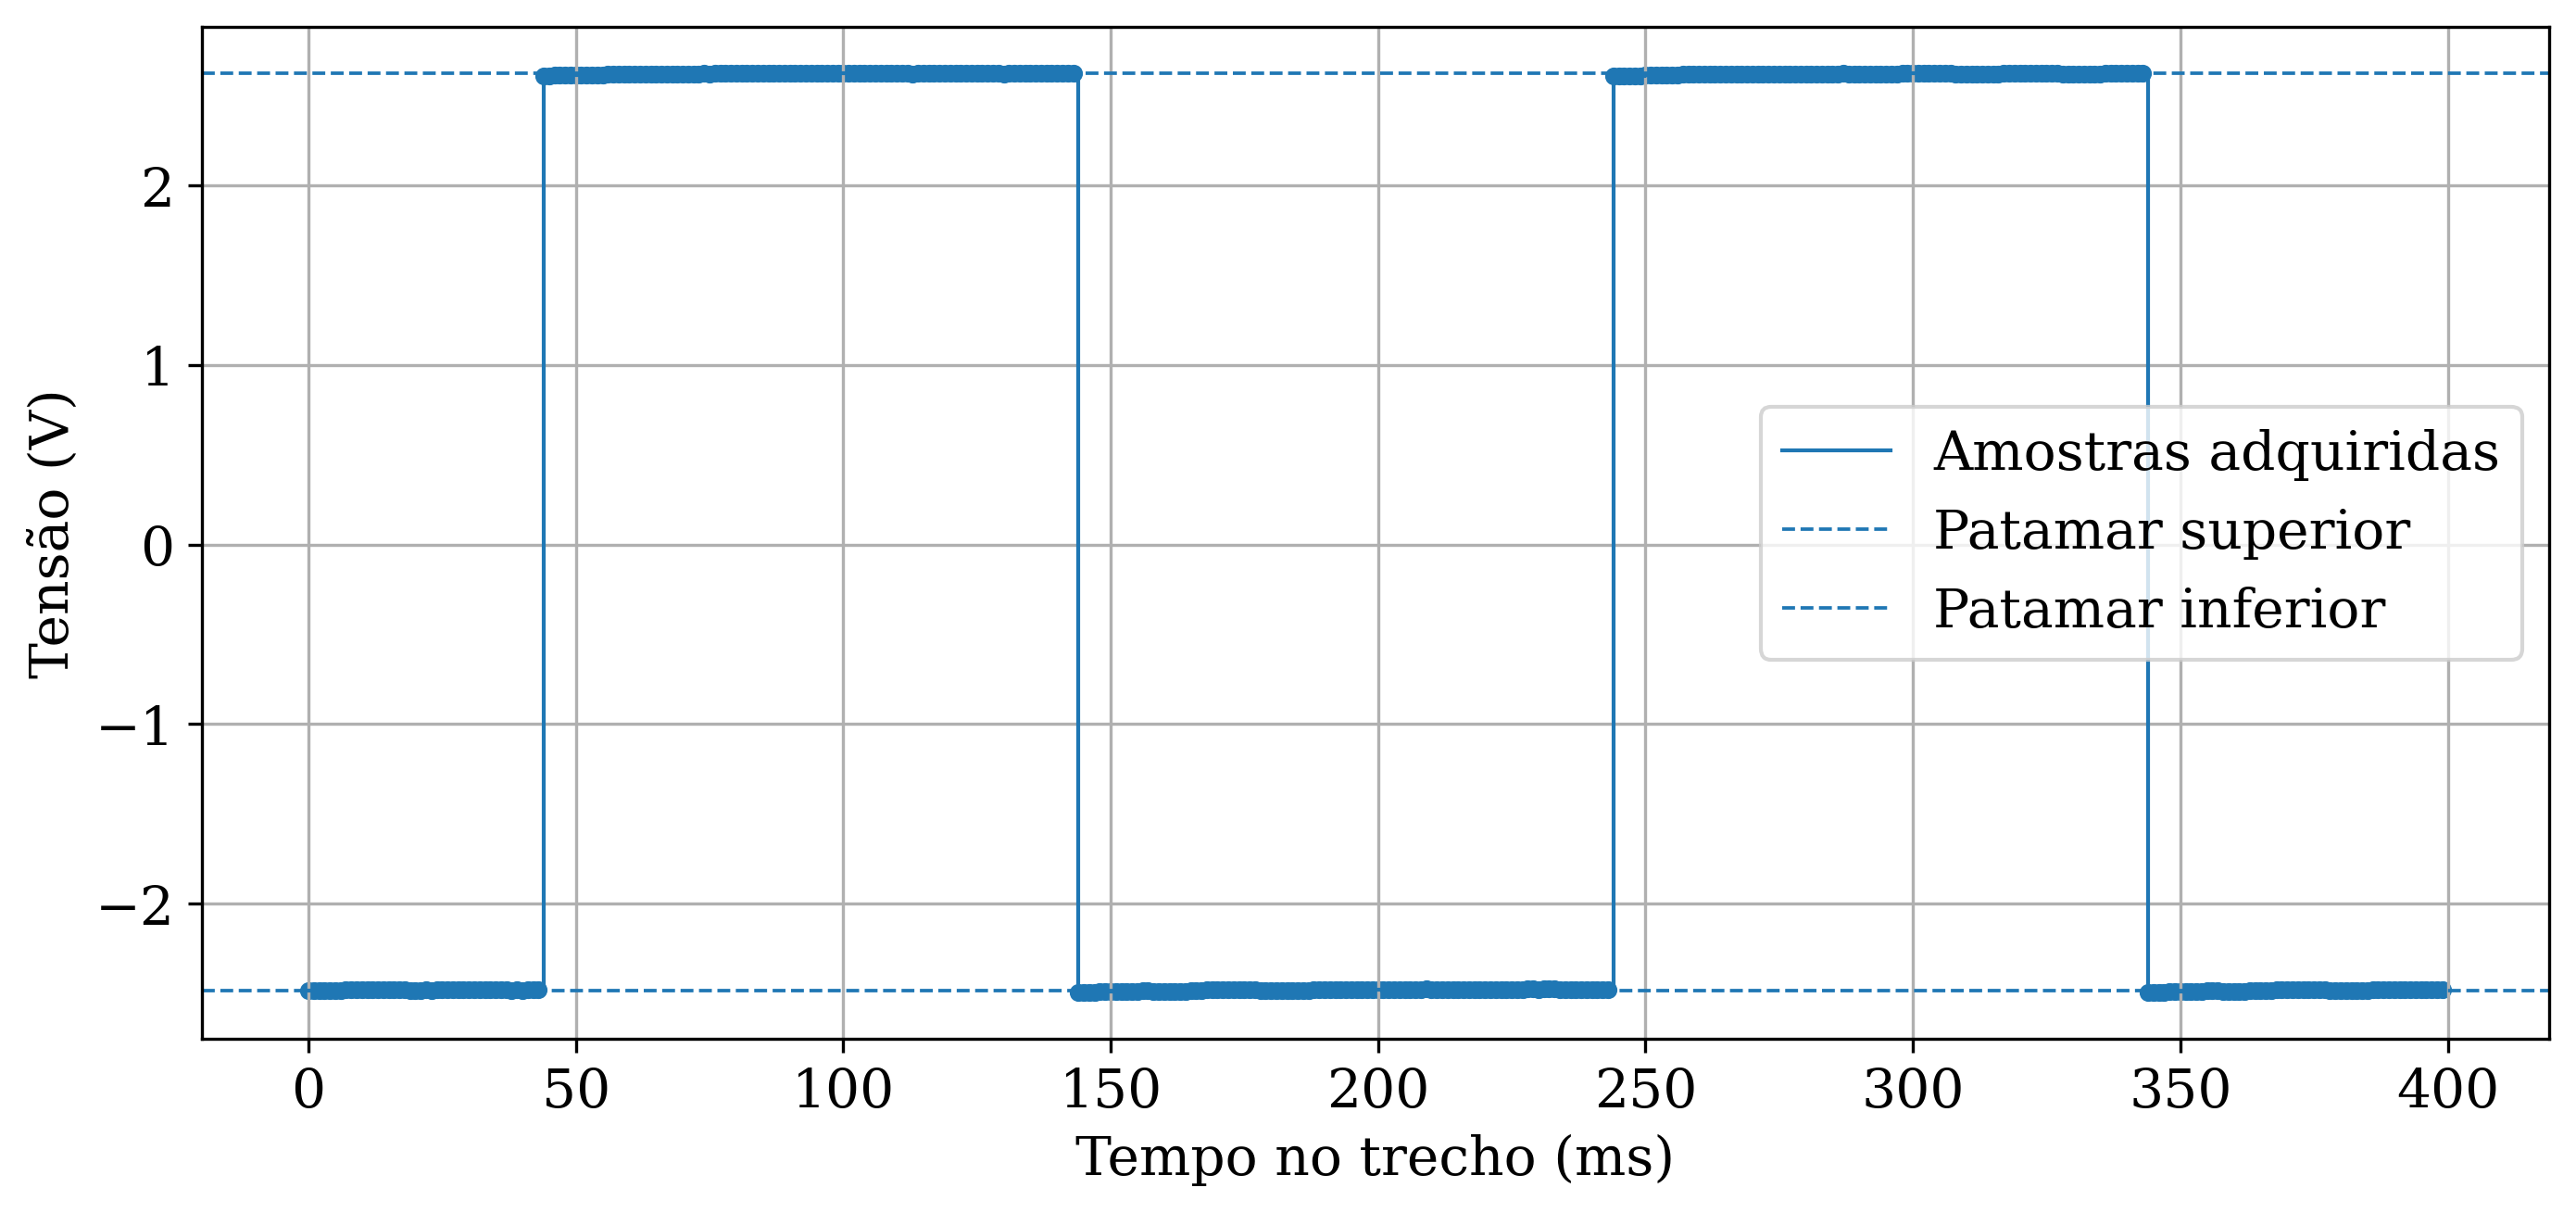
\includegraphics[width=\textwidth]
        {figuras/figura_tempo_5Hz.png}
        \small (a) Onda quadrada de 5~Hz em um trecho de 400~ms.
    \end{minipage}

    \medskip

    \begin{minipage}[t]{0.9\textwidth}
        \centering
        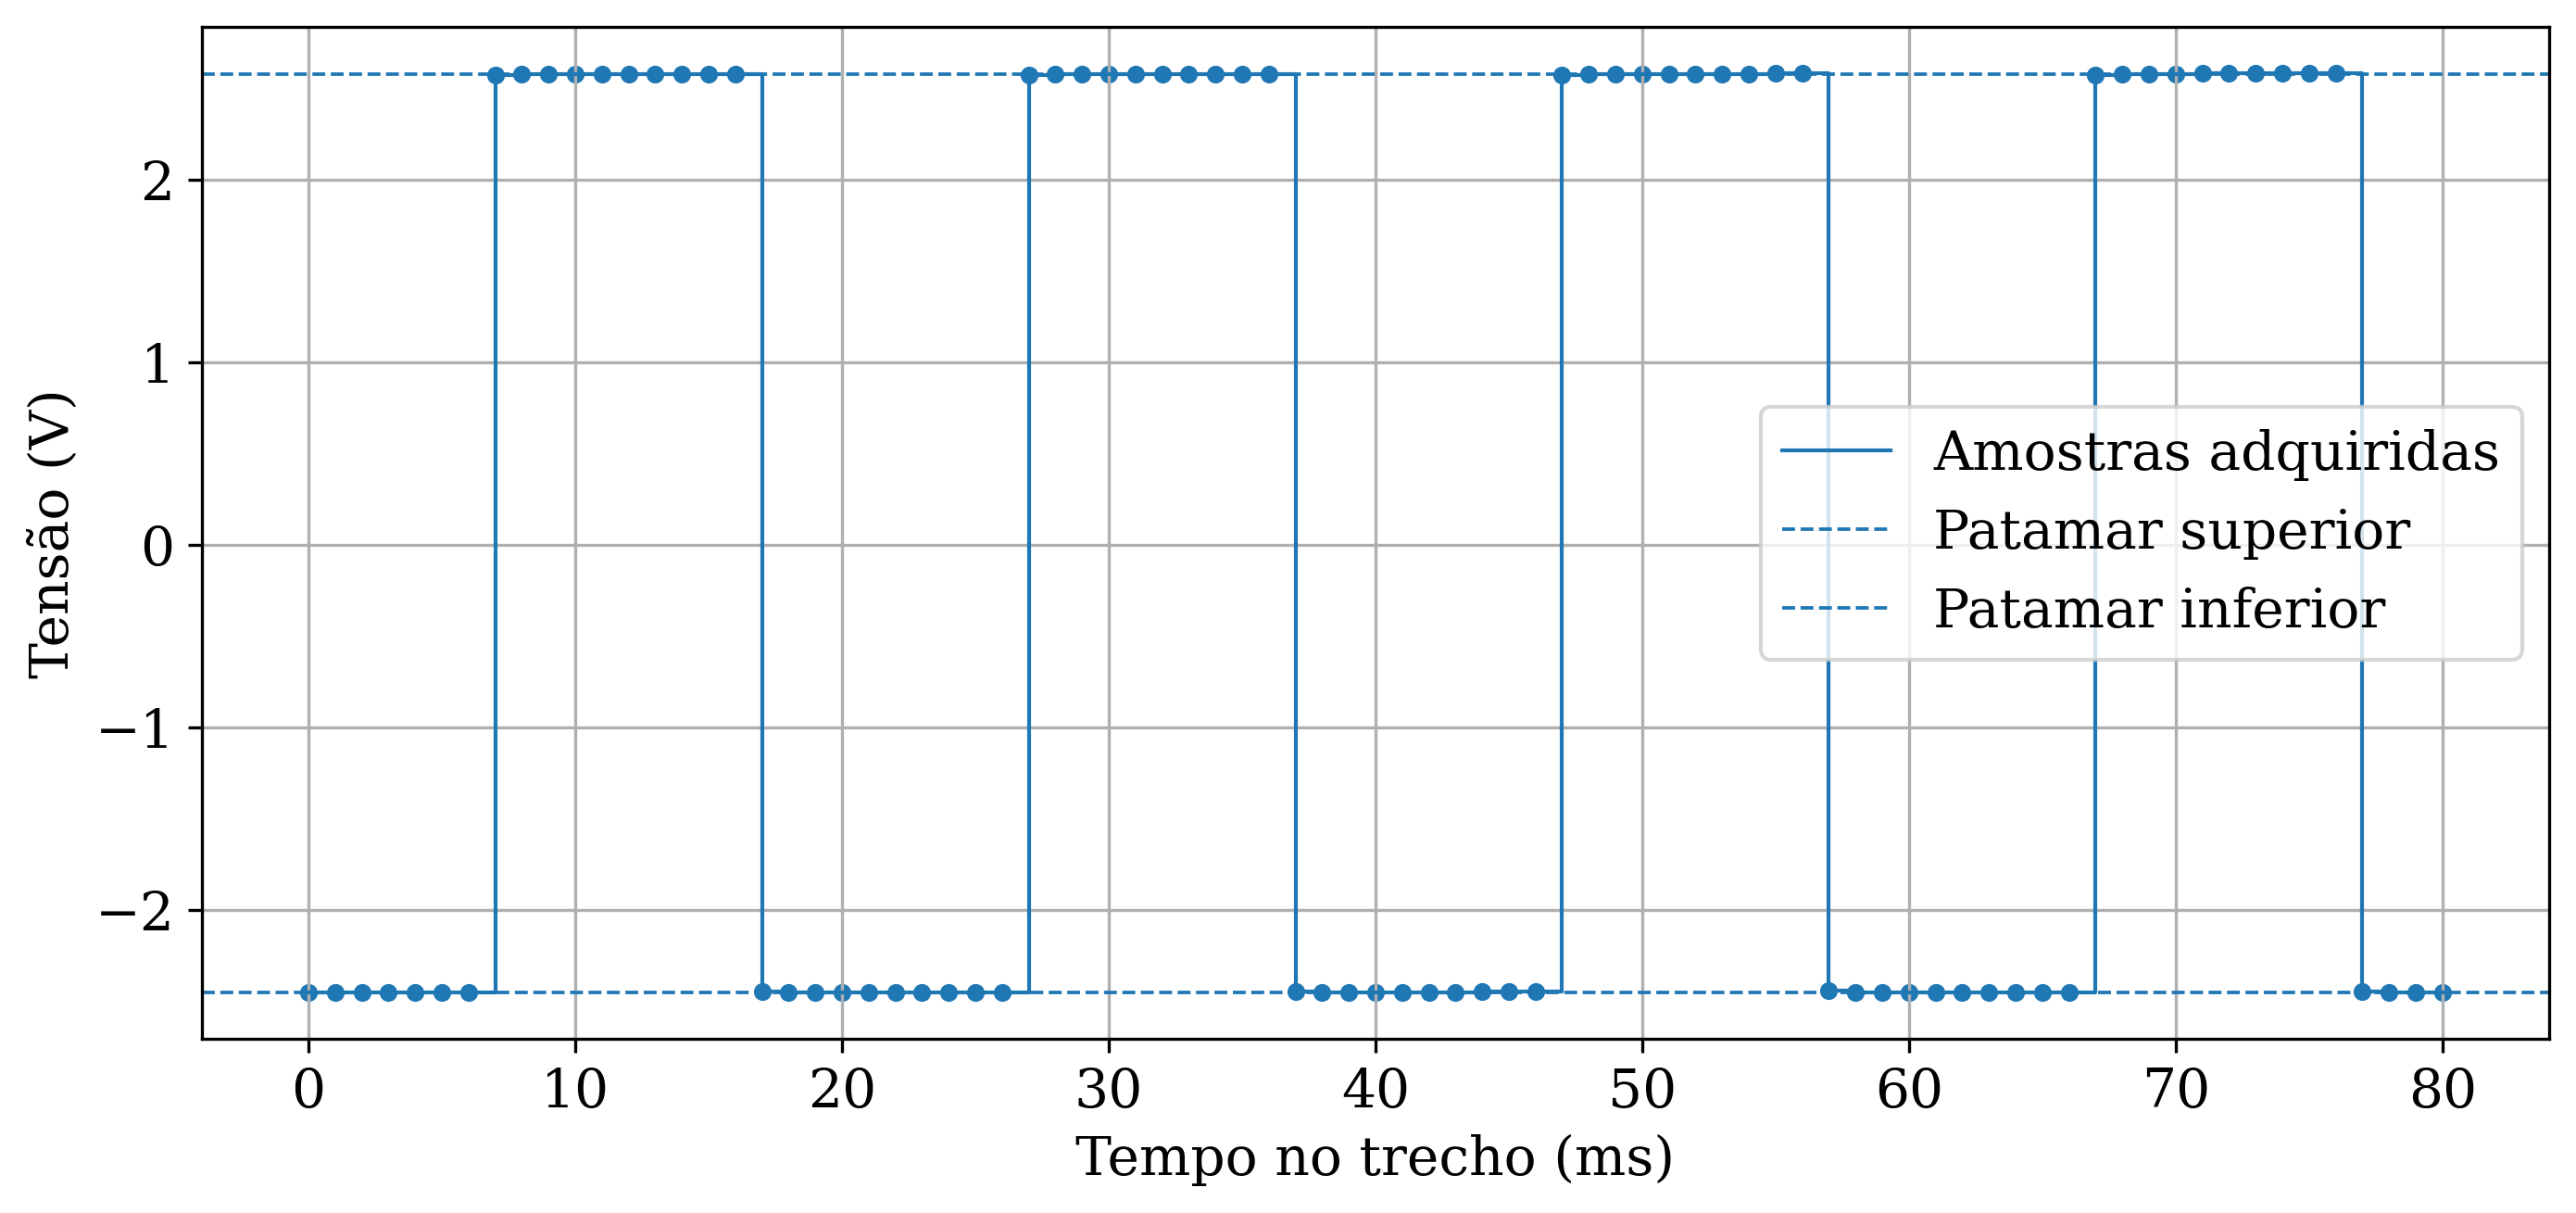
\includegraphics[width=\textwidth]
        {figuras/figura_tempo_50Hz.png}
        \small (b) Onda quadrada de 50~Hz em um trecho de 80~ms.
    \end{minipage}

    \caption[Ondas quadradas de 5 e 50~Hz no domínio do tempo]{
        Representação temporal das amostras adquiridas para ondas quadradas de (a) 5~Hz e (b) 50~Hz. Os marcadores indicam as amostras de tensão, enquanto as linhas contínuas auxiliam na visualização das transições entre os níveis lógicos. As linhas tracejadas horizontais representam os patamares superior e inferior estimados, situados em aproximadamente $+2,6$~V e $-2,5$~V, respectivamente. O sinal de 5~Hz apresenta período de aproximadamente 200~ms, enquanto o sinal de 50~Hz apresenta período de aproximadamente 20~ms; ambos possuem razão cíclica próxima de 50\%.
    }
    \label{fig:tempo_ondas_quadradas}
\end{figure}

A Figura~\ref{fig:tempo_comparativo_quadradas} apresenta os dois sinais em uma mesma base temporal. Durante o intervalo de aproximadamente 400~ms, foram observados dois períodos completos da onda de 5~Hz e aproximadamente vinte períodos da onda de 50~Hz, em concordância com a razão de dez entre suas frequências.

\begin{figure}[!htbp]
    \centering

    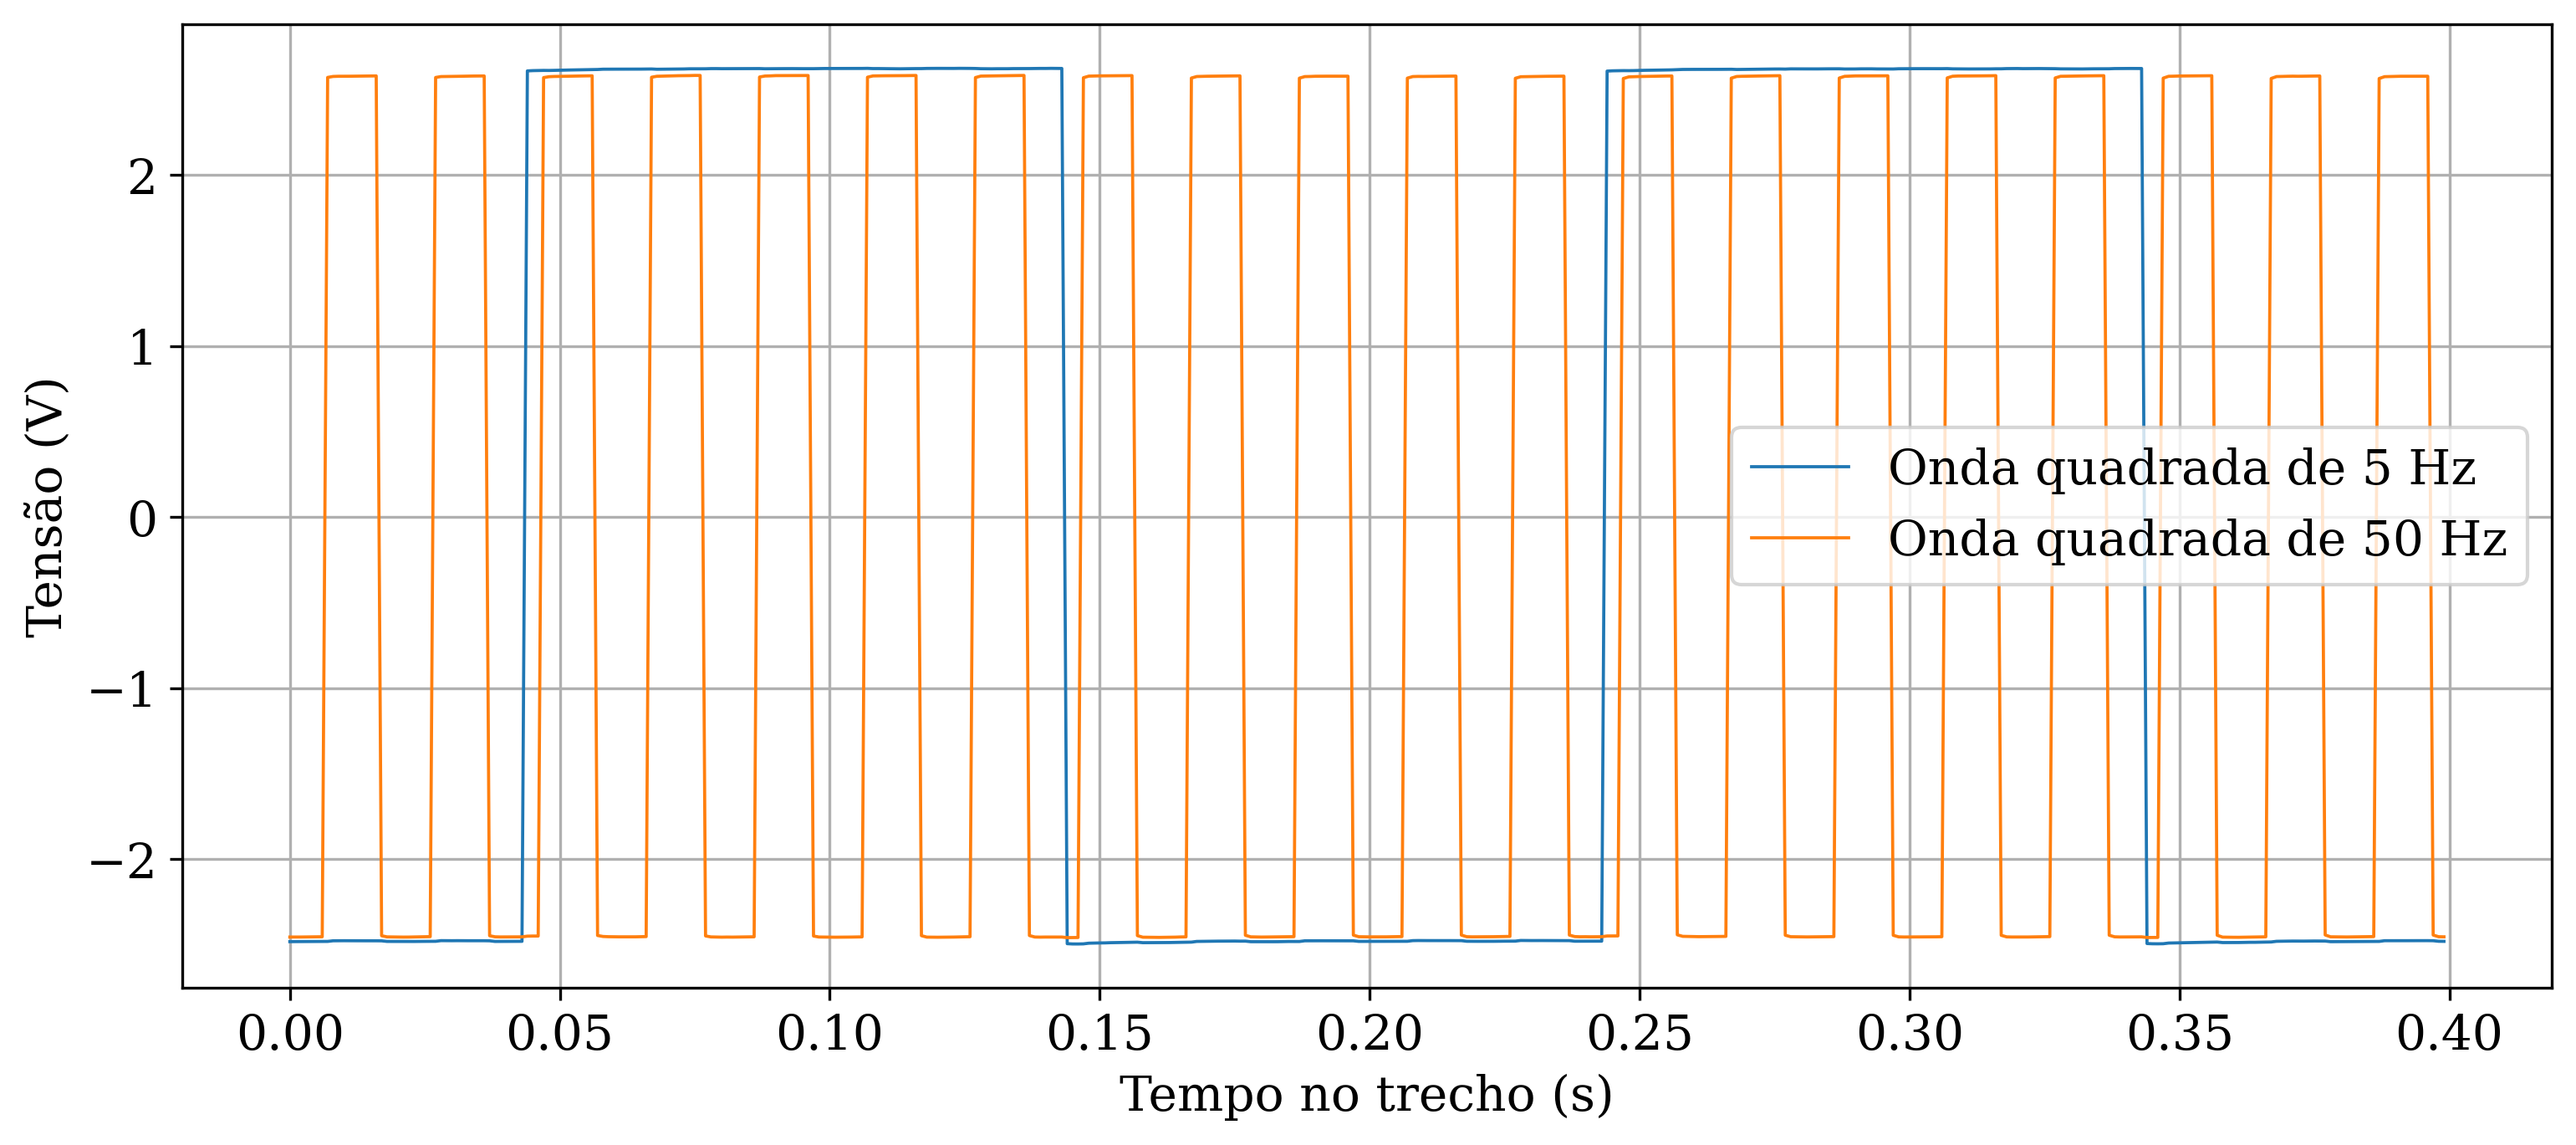
\includegraphics[width=\textwidth]{figuras/figura_tempo_comparativo_5Hz_50Hz.png}

    \caption[Comparação temporal de ondas quadradas de 5 e 50~Hz]{
        Comparação, em um intervalo de 400~ms, entre as ondas quadradas de 5~Hz e 50~Hz adquiridas simultaneamente. As curvas representam a evolução temporal das tensões amostradas, com patamares próximos de $+2,6$~V e $-2,5$~V e razão cíclica próxima de 50\%. Nesse intervalo, observam-se aproximadamente dois períodos do sinal de 5~Hz, cujo período é de 200~ms, e vinte períodos do sinal de 50~Hz, cujo período é de 20~ms, evidenciando a diferença de uma década entre as frequências dos sinais.
    }

    \label{fig:tempo_comparativo_quadradas}
\end{figure}

A comparação com um modelo quadrado ideal resultou em erro quadrático médio normalizado de 0,6852\% para a onda de 5~Hz e de 2,2335\% para a onda de 50~Hz. O aumento do erro no sinal de maior frequência esteve associado à maior proporção de amostras localizadas nas proximidades das transições e à redução da quantidade de pontos disponíveis em cada patamar.

Os tempos de subida entre 10\% e 90\% foram estimados em 0,8021~ms para a onda de 5~Hz e 0,8010~ms para a onda de 50~Hz. Os tempos de descida correspondentes foram de 0,7976~ms e 0,8002~ms. Entretanto, esses valores corresponderam a aproximadamente 0,8 amostra em todos os casos, uma vez que o intervalo nominal entre amostras foi próximo de 1~ms. Portanto, os resultados foram obtidos por interpolação entre duas amostras adjacentes e não devem ser interpretados como uma medição precisa do tempo analógico de transição. Nas duas ondas, a transição ocorreu entre uma amostra ainda localizada no patamar inferior e a amostra seguinte já posicionada no patamar superior, sem que fossem registrados pontos intermediários suficientes para caracterizar o formato real da borda.

Na onda de 5~Hz, o \textit{overshoot} global foi de 1,6310\% e o \textit{undershoot} global foi de 0,8811\%. Quando consideradas individualmente todas as transições, o \textit{overshoot} mediano foi nulo e o \textit{undershoot} mediano foi de 0,2996\%, indicando que os valores globais estiveram associados às maiores excursões observadas no registro e não ao comportamento típico de todas as bordas.

Para a onda de 50~Hz, o \textit{overshoot} global foi de 0,0829\% e o \textit{undershoot} global foi de 0,8756\%. As medianas por borda foram de 0\% e 0,0058\%, respectivamente. A reduzida quantidade de amostras nas transições também limita a detecção de picos transitórios estreitos, que podem ocorrer entre duas amostras consecutivas sem serem registrados pelo sistema.

O ruído eficaz combinado nos patamares correspondeu a aproximadamente 0,1170\% da amplitude da onda de 5~Hz e a 0,0443\% da amplitude da onda de 50~Hz. Os valores indicaram baixa dispersão das amostras enquanto os sinais permaneceram nos níveis inferior e superior.

A Tabela~\ref{tab:metricas_tempo_quadradas} reúne as principais métricas temporais obtidas para os dois sinais.

\begin{table}[!htbp]
    \centering
    \caption{Principais métricas no domínio do tempo para as ondas quadradas de 5~Hz e 50~Hz.}
    \label{tab:metricas_tempo_quadradas}
    \small
    \begin{tabular}{l c c}
        \hline
        \textbf{Métrica} & \textbf{5~Hz} & \textbf{50~Hz} \\
        \hline
        Patamar inferior (V)      & $-2,4805$ & $-2,4545$ \\
        Patamar superior (V)      & $2,6217$  & $2,5792$  \\
        Amplitude (V)             & $5,1022$  & $5,0337$  \\
        Frequência (Hz)           & $4,99995$ & $49,99964$ \\
        Período (ms)              & $200,0020$ & $20,0001$ \\
        Ciclo de trabalho (\%)    & $49,9978$ & $49,9913$ \\
        RMS (V)                   & $2,5512$  & $2,5105$  \\
        Amostras por período      & $200,03$  & $20,00$   \\
        \hline
    \end{tabular}
\end{table}

As medições realizadas pelo osciloscópio indicaram frequências de 5,00~Hz e 50,00~Hz e ciclos de trabalho de 50\% para os dois sinais. Para a onda de 5~Hz, o osciloscópio registrou patamares de aproximadamente $-2,64$~V e 2,32~V, amplitude entre patamares de 4,96~V, amplitude pico a pico de 5,28~V e valor eficaz de 2,47~V. Para a onda de 50~Hz, foram registrados patamares de aproximadamente $-2,64$~V e 2,24~V, amplitude entre patamares de 4,88~V, amplitude pico a pico de 5,20~V e valor eficaz de 2,45~V.

Em relação ao osciloscópio, as amplitudes entre patamares obtidas pelo sistema foram 2,87\% superiores para a onda de 5~Hz e 3,15\% superiores para a onda de 50~Hz. As amplitudes pico a pico totais foram 0,94\% e 2,27\% inferiores às referências, respectivamente. Os valores eficazes medidos pelo sistema foram 3,29\% superiores para 5~Hz e 2,47\% superiores para 50~Hz.

A Tabela~\ref{tab:comparacao_osciloscopio_quadradas} sintetiza a comparação das principais medidas temporais. Os tempos de subida e descida não foram incluídos como medidas diretamente comparáveis, pois a taxa de aquisição do sistema não forneceu resolução suficiente para caracterizar as transições com a mesma precisão do osciloscópio.

\begin{table}[!htbp]
    \centering
    \caption{Comparação entre as principais métricas das ondas quadradas obtidas pelo sistema e pelo osciloscópio.}
    \label{tab:comparacao_osciloscopio_quadradas}
    \begin{tabularx}{\textwidth}{l c c c c}
        \hline
        \multirow{2}{*}{\textbf{Métricas}} &
        \multicolumn{2}{c}{\textbf{5~Hz}} &
        \multicolumn{2}{c}{\textbf{50~Hz}} \\
        &
        \textbf{Sistema} &
        \textbf{Osciloscópio} &
        \textbf{Sistema} &
        \textbf{Osciloscópio} \\
        \hline
        Amplitude entre patamares (V)
            & 5,1022 & 4,9600 & 5,0337 & 4,8800 \\
        Pico a pico (V)
            & 5,2304 & 5,2800 & 5,0819 & 5,2000 \\
        RMS (V)
            & 2,5512 & 2,4700 & 2,5105 & 2,4500 \\
        Ciclo de trabalho (\%)
            & 49,9978 & 50,0000 & 49,9913 & 50,0000 \\
        \hline
    \end{tabularx}

\end{table}

\subsubsection{Resultados no domínio da frequência}
\label{subsubsec:quadradas_frequencia}

Os espectros confirmaram a componente fundamental e a sequência de harmônicas ímpares esperada para uma onda quadrada simétrica, cujas frequências obedecem à relação $f_n=n f_0$, com $n=1,3,5,\ldots$. Dessa forma, o espaçamento entre componentes ímpares consecutivas foi de 10~Hz para o sinal de 5~Hz e de 100~Hz para o sinal de 50~Hz. As frequências e amplitudes das cinco primeiras componentes são reunidas na Tabela~\ref{tab:harmonicas_quadradas}.

A Figura~\ref{fig:espectros_quadradas} apresenta os espectros em escala linear e em dBc. A primeira representação evidencia a redução da amplitude com o aumento da ordem harmônica, enquanto a normalização pela fundamental permite comparar diretamente os dois sinais.

\begin{figure}[!htbp]
\centering

\begin{minipage}[t]{0.9\textwidth}
    \centering
    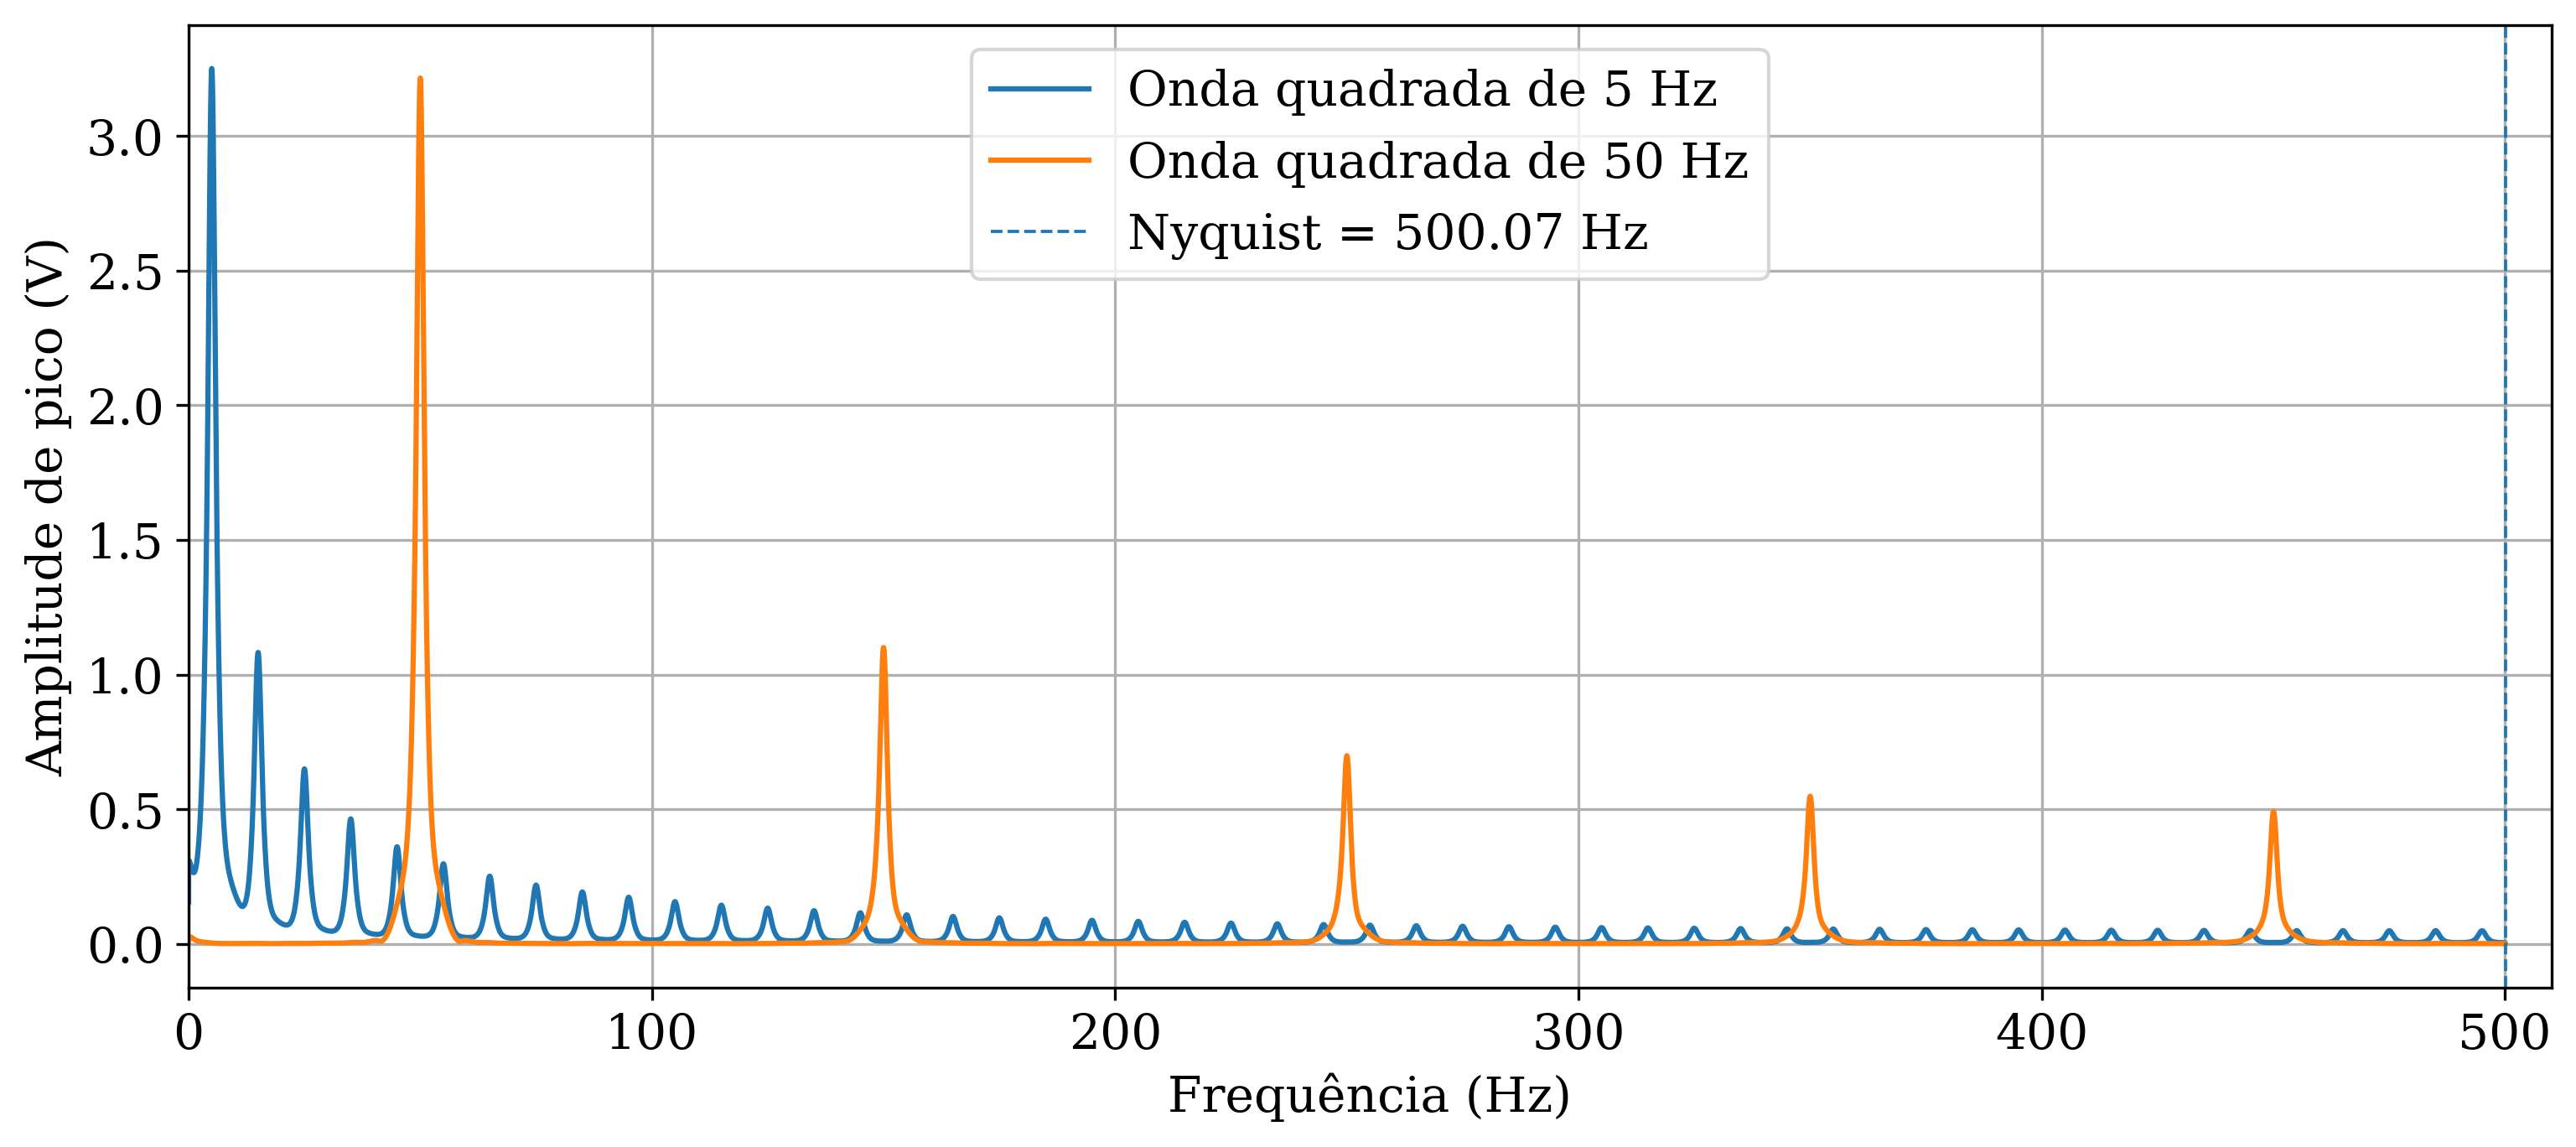
\includegraphics[width=\textwidth]{figuras/figura_espectro_linear_5Hz_50Hz.png}

    \small (a) Espectros em amplitude de pico, na escala linear.
\end{minipage}

\medskip

\begin{minipage}[t]{0.9\textwidth}
    \centering
    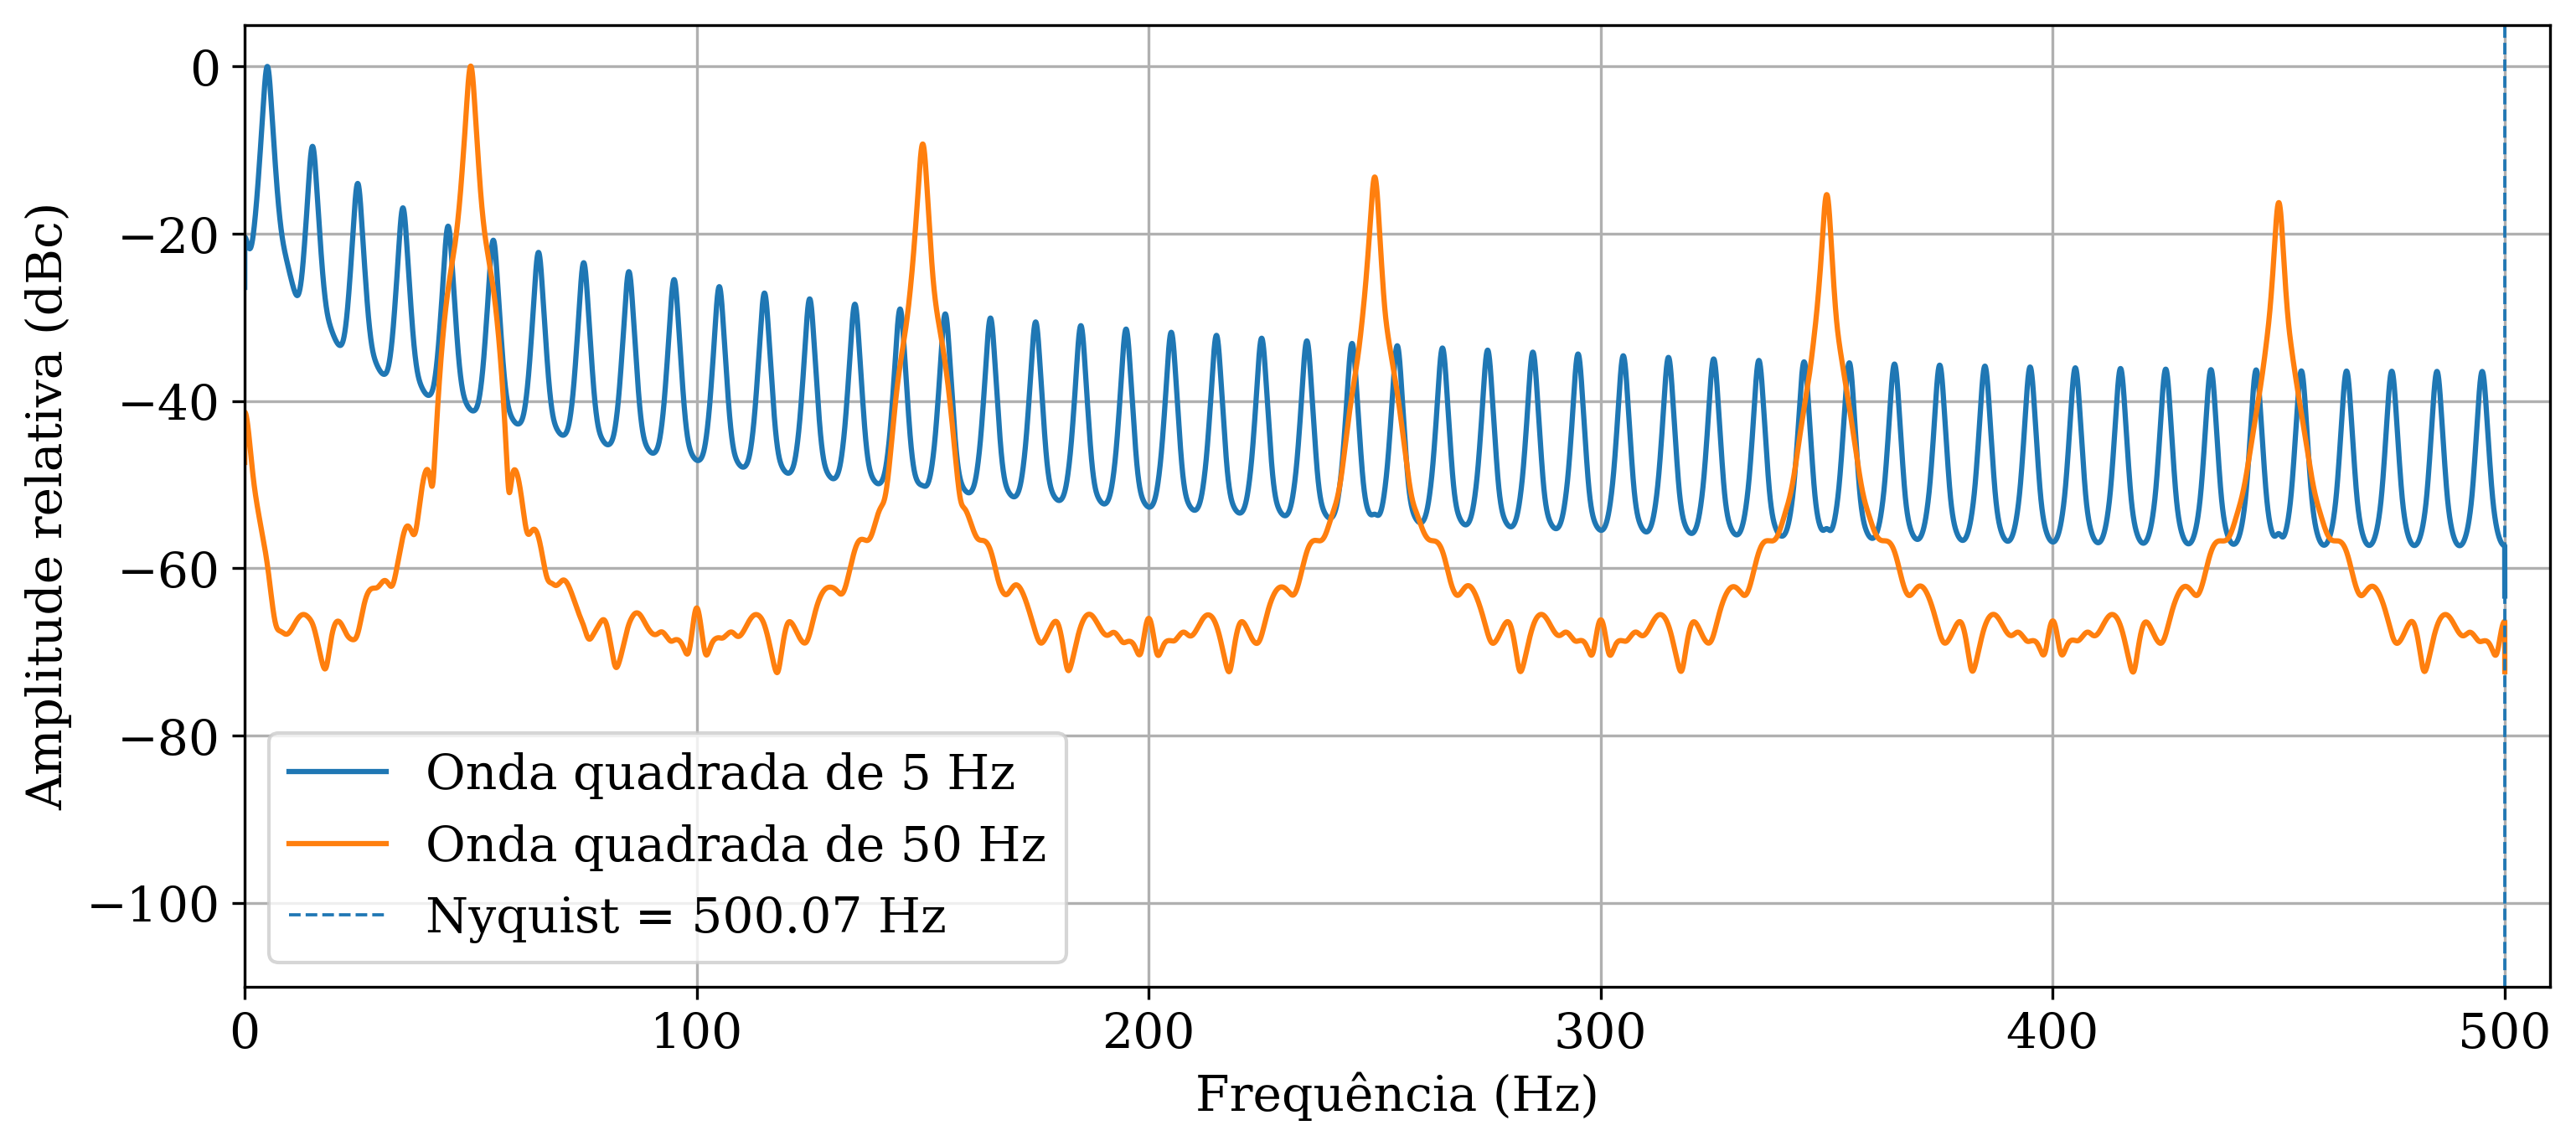
\includegraphics[width=\textwidth]{figuras/figura_espectro_dbc_5Hz_50Hz.png}

    \small (b) Espectros normalizados em relação às respectivas componentes fundamentais, em dBc.
\end{minipage}

\caption[Espectros das ondas quadradas de 5 e 50~Hz]{
    Espectros de frequência das ondas quadradas de 5~Hz e 50~Hz, adquiridas com frequência de amostragem de aproximadamente 1~kHz. Em (a), são apresentadas as amplitudes de pico em escala linear; em (b), cada espectro é normalizado pela respectiva componente fundamental, definida como 0~dBc. A linha vertical tracejada em 500,07~Hz indica a frequência de Nyquist e o limite superior da faixa espectral analisada.
}

\label{fig:espectros_quadradas}

\end{figure}

As amplitudes de pico das componentes fundamentais foram de 3,2477~V e 3,1962~V para as ondas de 5~Hz e 50~Hz, respectivamente. No primeiro caso, as harmônicas analisadas permaneceram a menos de 0,06~dB dos valores ideais. No segundo, a atenuação adicional aumentou com a ordem, passando de aproximadamente 0,19~dB na terceira harmônica para 1,55~dB na nona.

A Figura~\ref{fig:harmonicas_impares_quadradas} sintetiza essa comparação. O sinal de 5~Hz permaneceu praticamente sobreposto à resposta teórica, enquanto o de 50~Hz apresentou afastamento crescente nas frequências mais elevadas.

\begin{figure}[!htbp]
\centering

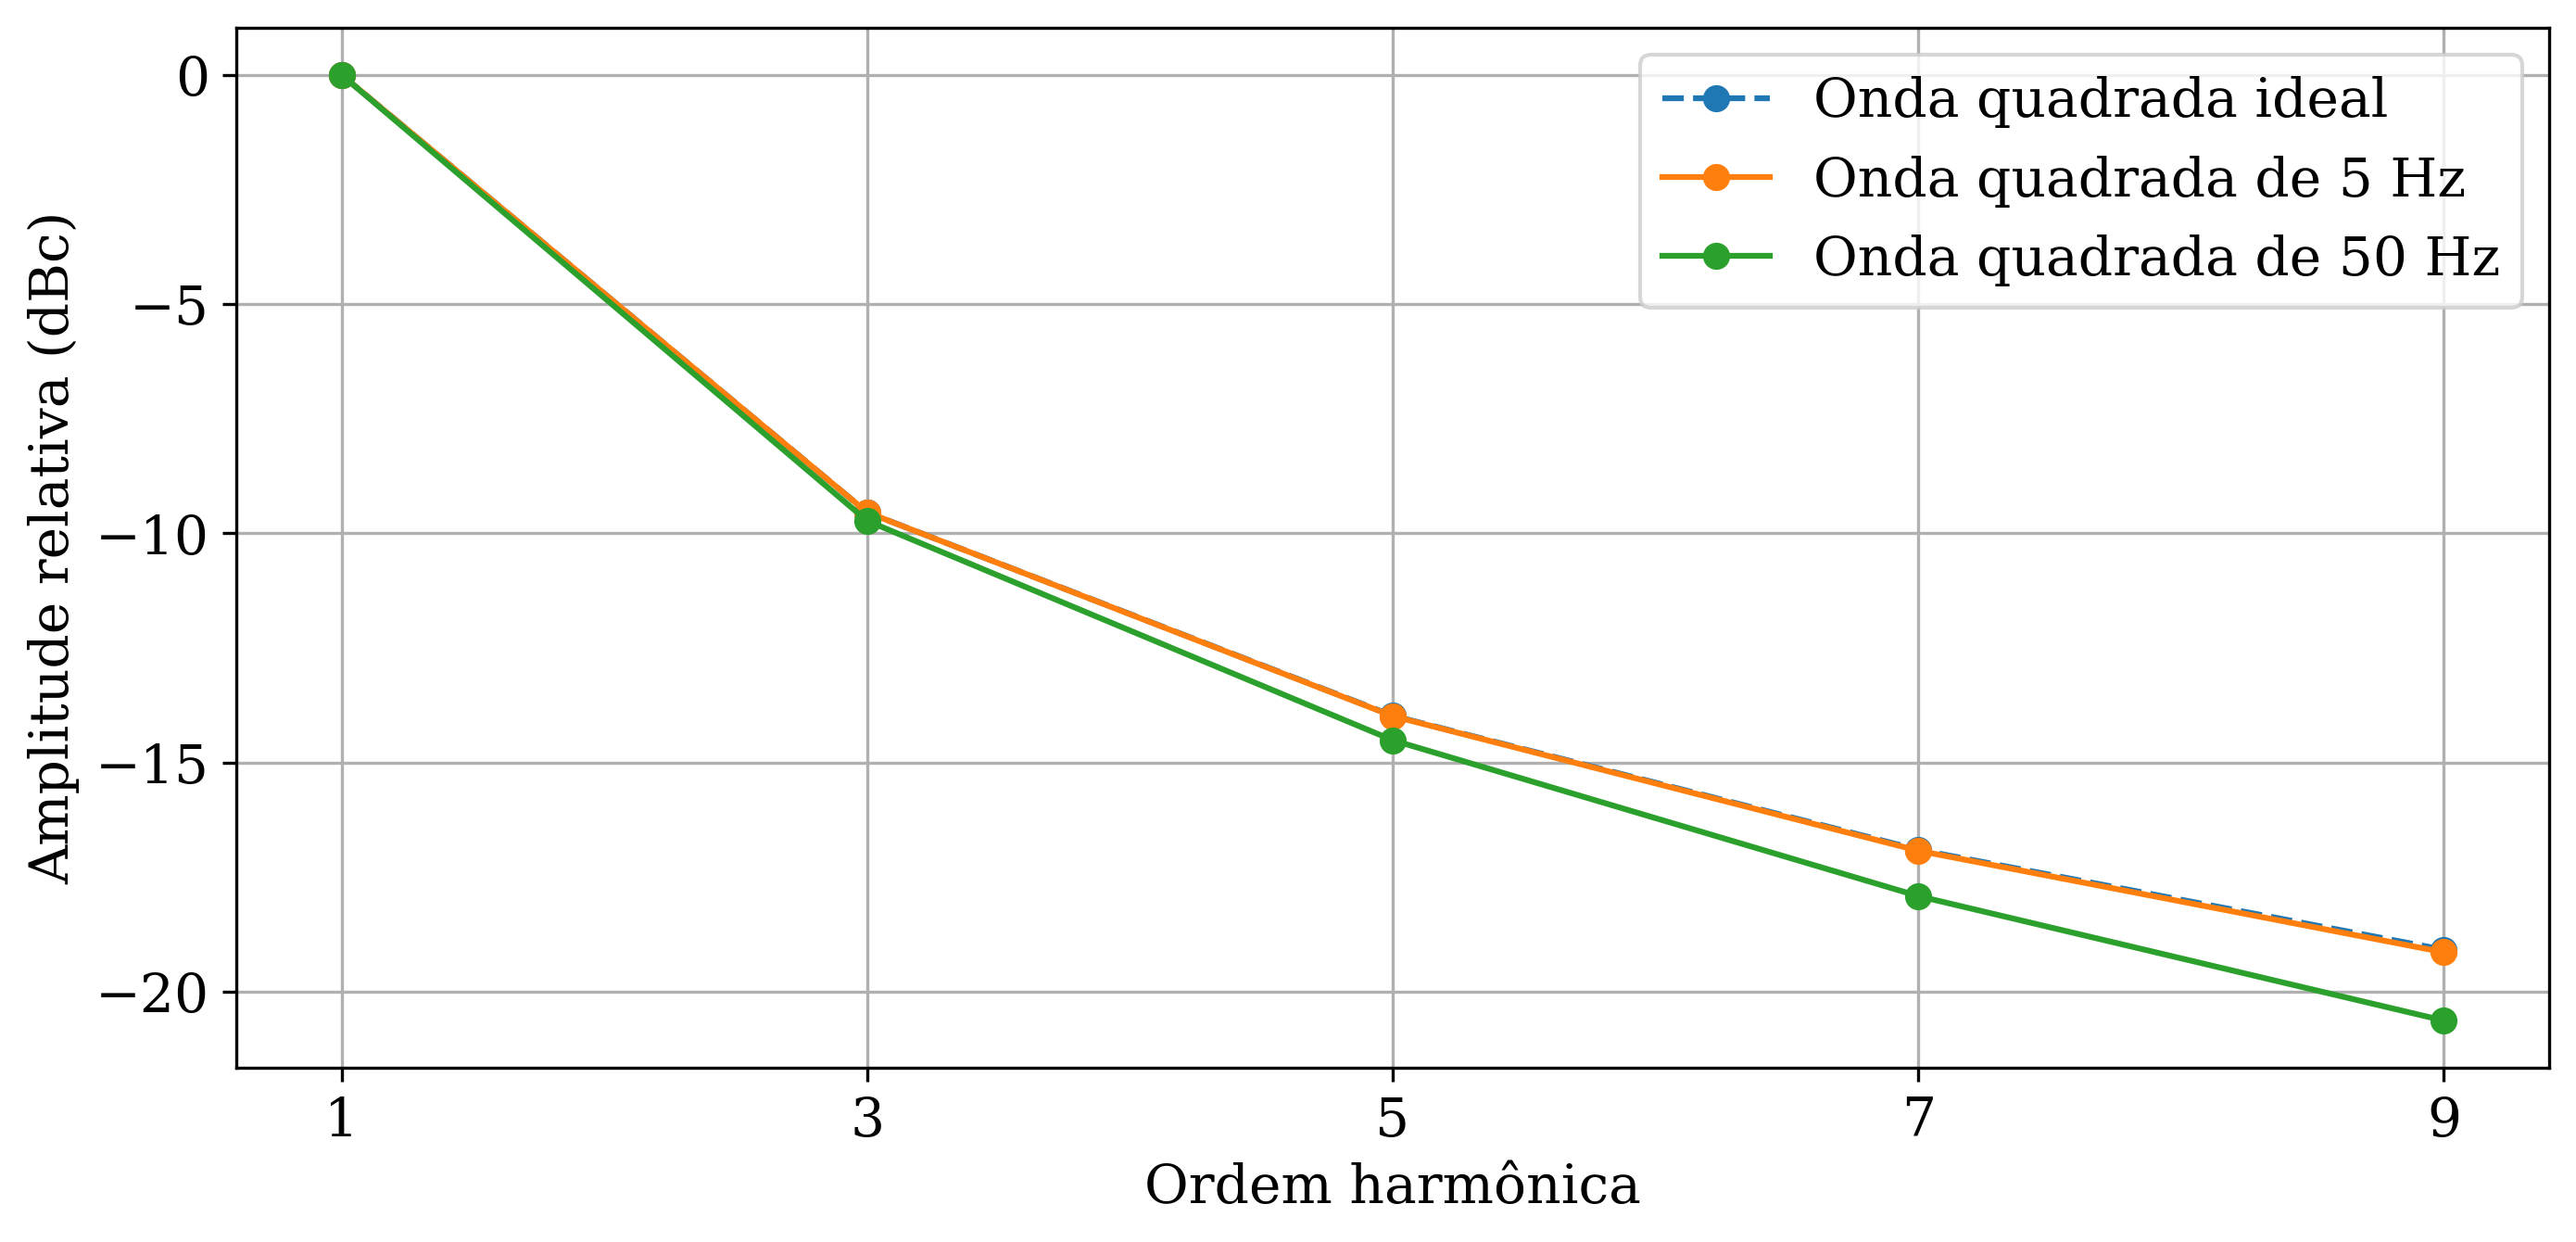
\includegraphics[width=\textwidth]{figuras/figura_harmonicas_impares_5Hz_50Hz.png}

\caption[Harmônicas ímpares das ondas quadradas de 5 e 50~Hz]{
    Comparação entre as amplitudes relativas das cinco primeiras componentes ímpares das ondas quadradas de 5~Hz e 50~Hz e a resposta de uma onda quadrada ideal. Os níveis foram normalizados pela fundamental, definida como 0~dBc. Para o modelo ideal, a amplitude decresce proporcionalmente a $1/n$, ou seja, o nível relativo é dado por $-20\log_{10}(n)$.
}

\label{fig:harmonicas_impares_quadradas}

\end{figure}

A Tabela~\ref{tab:harmonicas_quadradas} reúne as frequências nominais e os níveis relativos utilizados na comparação.

\begin{table}[!htbp]
    \centering
    
    \caption{Frequências e amplitudes relativas das primeiras harmônicas ímpares das ondas quadradas.}
    \label{tab:harmonicas_quadradas}
    \small
    
    \setlength{\tabcolsep}{5pt}
    \begin{tabular}{c c c c c c}
        \hline
        \textbf{Ordem} &
        \textbf{Ideal} &
        \multicolumn{2}{c}{\textbf{Onda de 5~Hz}} &
        \multicolumn{2}{c}{\textbf{Onda de 50~Hz}} \\
        \textbf{harmônica} &
        \textbf{(dBc)} &
        \textbf{Frequência (Hz)} &
        \textbf{Nível (dBc)} &
        \textbf{Frequência (Hz)} &
        \textbf{Nível (dBc)} \\
        \hline
        1 & 0,0000     & 5   & 0,0000     & 50  & 0,0000 \\
        3 & $-9,5424$  & 15  & $-9,5435$  & 150 & $-9,7278$ \\
        5 & $-13,9794$ & 25  & $-13,9879$ & 250 & $-14,5136$ \\
        7 & $-16,9020$ & 35  & $-16,9244$ & 350 & $-17,9139$ \\
        9 & $-19,0849$ & 45  & $-19,1396$ & 450 & $-20,6304$ \\
        \hline
    \end{tabular}
\end{table}

As harmônicas pares apresentaram níveis reduzidos. A segunda harmônica foi a maior entre as primeiras ordens, atingindo aproximadamente $-57,54$~dBc em 10~Hz no sinal de 5~Hz e $-66,64$~dBc em 100~Hz no sinal de 50~Hz. Esse resultado é compatível com o ciclo de trabalho próximo de 50\% e com a simetria entre os semiciclos.

No canal de 5~Hz, a principal componente não associada à sequência ímpar prevista apareceu em 249,96~Hz, com aproximadamente $-53,53$~dBc. Componentes mais fracas também ocorreram nas proximidades de 350~Hz e 450~Hz. Como essas frequências coincidem com harmônicas do sinal de 50~Hz adquirido simultaneamente, os resultados sugerem possível acoplamento entre canais, embora o ensaio não permita confirmar essa origem.

No canal de 50~Hz, as maiores componentes espúrias ocorreram em 40,37~Hz e 59,72~Hz, ambas em torno de $-48,2$~dBc, enquanto as demais permaneceram abaixo de aproximadamente $-54,9$~dBc. A proximidade de uma delas com 60~Hz sugere contribuição da rede elétrica, mas o registro isolado não permite determinar sua origem.

A menor frequência fundamental do sinal de 5~Hz manteve diversas harmônicas ímpares abaixo da frequência de Nyquist, preservando uma parcela maior de seu conteúdo espectral. Para o sinal de 50~Hz, somente as componentes até a nona ordem permaneceram diretamente abaixo de 500,07~Hz; as ordens superiores ultrapassaram esse limite e ficaram sujeitas a aliasing.

\subsubsection{Discussão dos resultados}
\label{subsubsec:discussao_quadradas}

Os dois sinais apresentaram frequências, períodos e ciclos de trabalho muito próximos aos valores configurados. Os erros relativos de frequência permaneceram inferiores a 0,002\%, e os desvios do ciclo de trabalho em relação a 50\% foram menores que 0,01 ponto percentual. Esses resultados indicam que a organização temporal dos patamares foi preservada nas duas condições avaliadas.

As amplitudes entre patamares permaneceram próximas dos 5~V configurados no gerador, com desvios de aproximadamente 2,04\% para a onda de 5~Hz e 0,67\% para a de 50~Hz. As diferenças em relação ao osciloscópio foram um pouco maiores porque os níveis medidos pelos dois equipamentos não eram perfeitamente simétricos em torno de zero e porque as métricas de amplitude entre patamares e de pico a pico respondem de maneira distinta às excursões transitórias.

Os patamares foram preservados sem arredondamento gradual claramente resolvido pelas amostras. Isso, contudo, não demonstra que as bordas analógicas fossem instantâneas. Com período de amostragem próximo de 1~ms, as transições ocorreram entre pontos adjacentes, impedindo a caracterização precisa de tempos de subida ou descida dessa mesma ordem ou inferiores.

O osciloscópio indicou tempos de subida e descida próximos de 2~ms, enquanto a interpolação das amostras do sistema resultou em cerca de 0,8~ms. A diferença decorre da baixa quantidade de pontos nas transições e dos métodos de medição empregados, não de uma resposta mais rápida da plataforma. Pela mesma razão, os valores de \textit{overshoot} e \textit{undershoot} calculados pelo sistema podem subestimar excursões estreitas registradas pelo osciloscópio.

No domínio da frequência, a onda de 5~Hz reproduziu as primeiras harmônicas ímpares com elevada concordância em relação ao modelo ideal. Como sua fundamental estava distante do limite de Nyquist, um número maior de componentes permaneceu disponível para representar as transições e os patamares.

Para a onda de 50~Hz, o afastamento em relação ao modelo aumentou com a ordem harmônica, em consonância com a aproximação ao limite superior da banda, a resposta em frequência da cadeia de aquisição e a menor quantidade de amostras por período. A nona harmônica, em 450~Hz, ficou a apenas cerca de 50~Hz da frequência de Nyquist, enquanto as componentes a partir da décima primeira ordem ficaram sujeitas a aliasing.

De forma geral, a plataforma adquiriu adequadamente as duas ondas quadradas, preservando seus níveis, períodos, ciclos de trabalho e principais componentes espectrais. A onda de 5~Hz apresentou maior concordância com a distribuição ideal, ao passo que a de 50~Hz evidenciou as limitações de banda impostas pela taxa de amostragem.


% ----------------------------------------------------------------------------
\subsection{Sinal multitom}
\label{subsec:sinal_multitom}

O sinal multitom foi produzido no primeiro canal do gerador Politerm POL-40 com frequência-base de 50~Hz, amplitude pico a pico configurada em 5~V e componente contínua nula. A forma de onda gerada foi constituída por cinco componentes senoidais principais, localizadas nominalmente em 50, 100, 150, 200 e 250~Hz. A aquisição foi realizada simultaneamente ao sinal sinc, aplicado ao segundo canal do sistema, com taxa nominal de 1~kS/s por canal.

A Figura~\ref{fig:configuracao_gerador_multitom_sinc} apresenta a configuração utilizada no gerador para os dois sinais complexos. No primeiro canal, observa-se a seleção da forma de onda multitom, enquanto o segundo canal foi configurado para produzir o sinal sinc. Ambos os canais foram ajustados para 50~Hz, amplitude de 5~V e offset de 0~V.

\begin{figure}[!htbp]
    \centering

    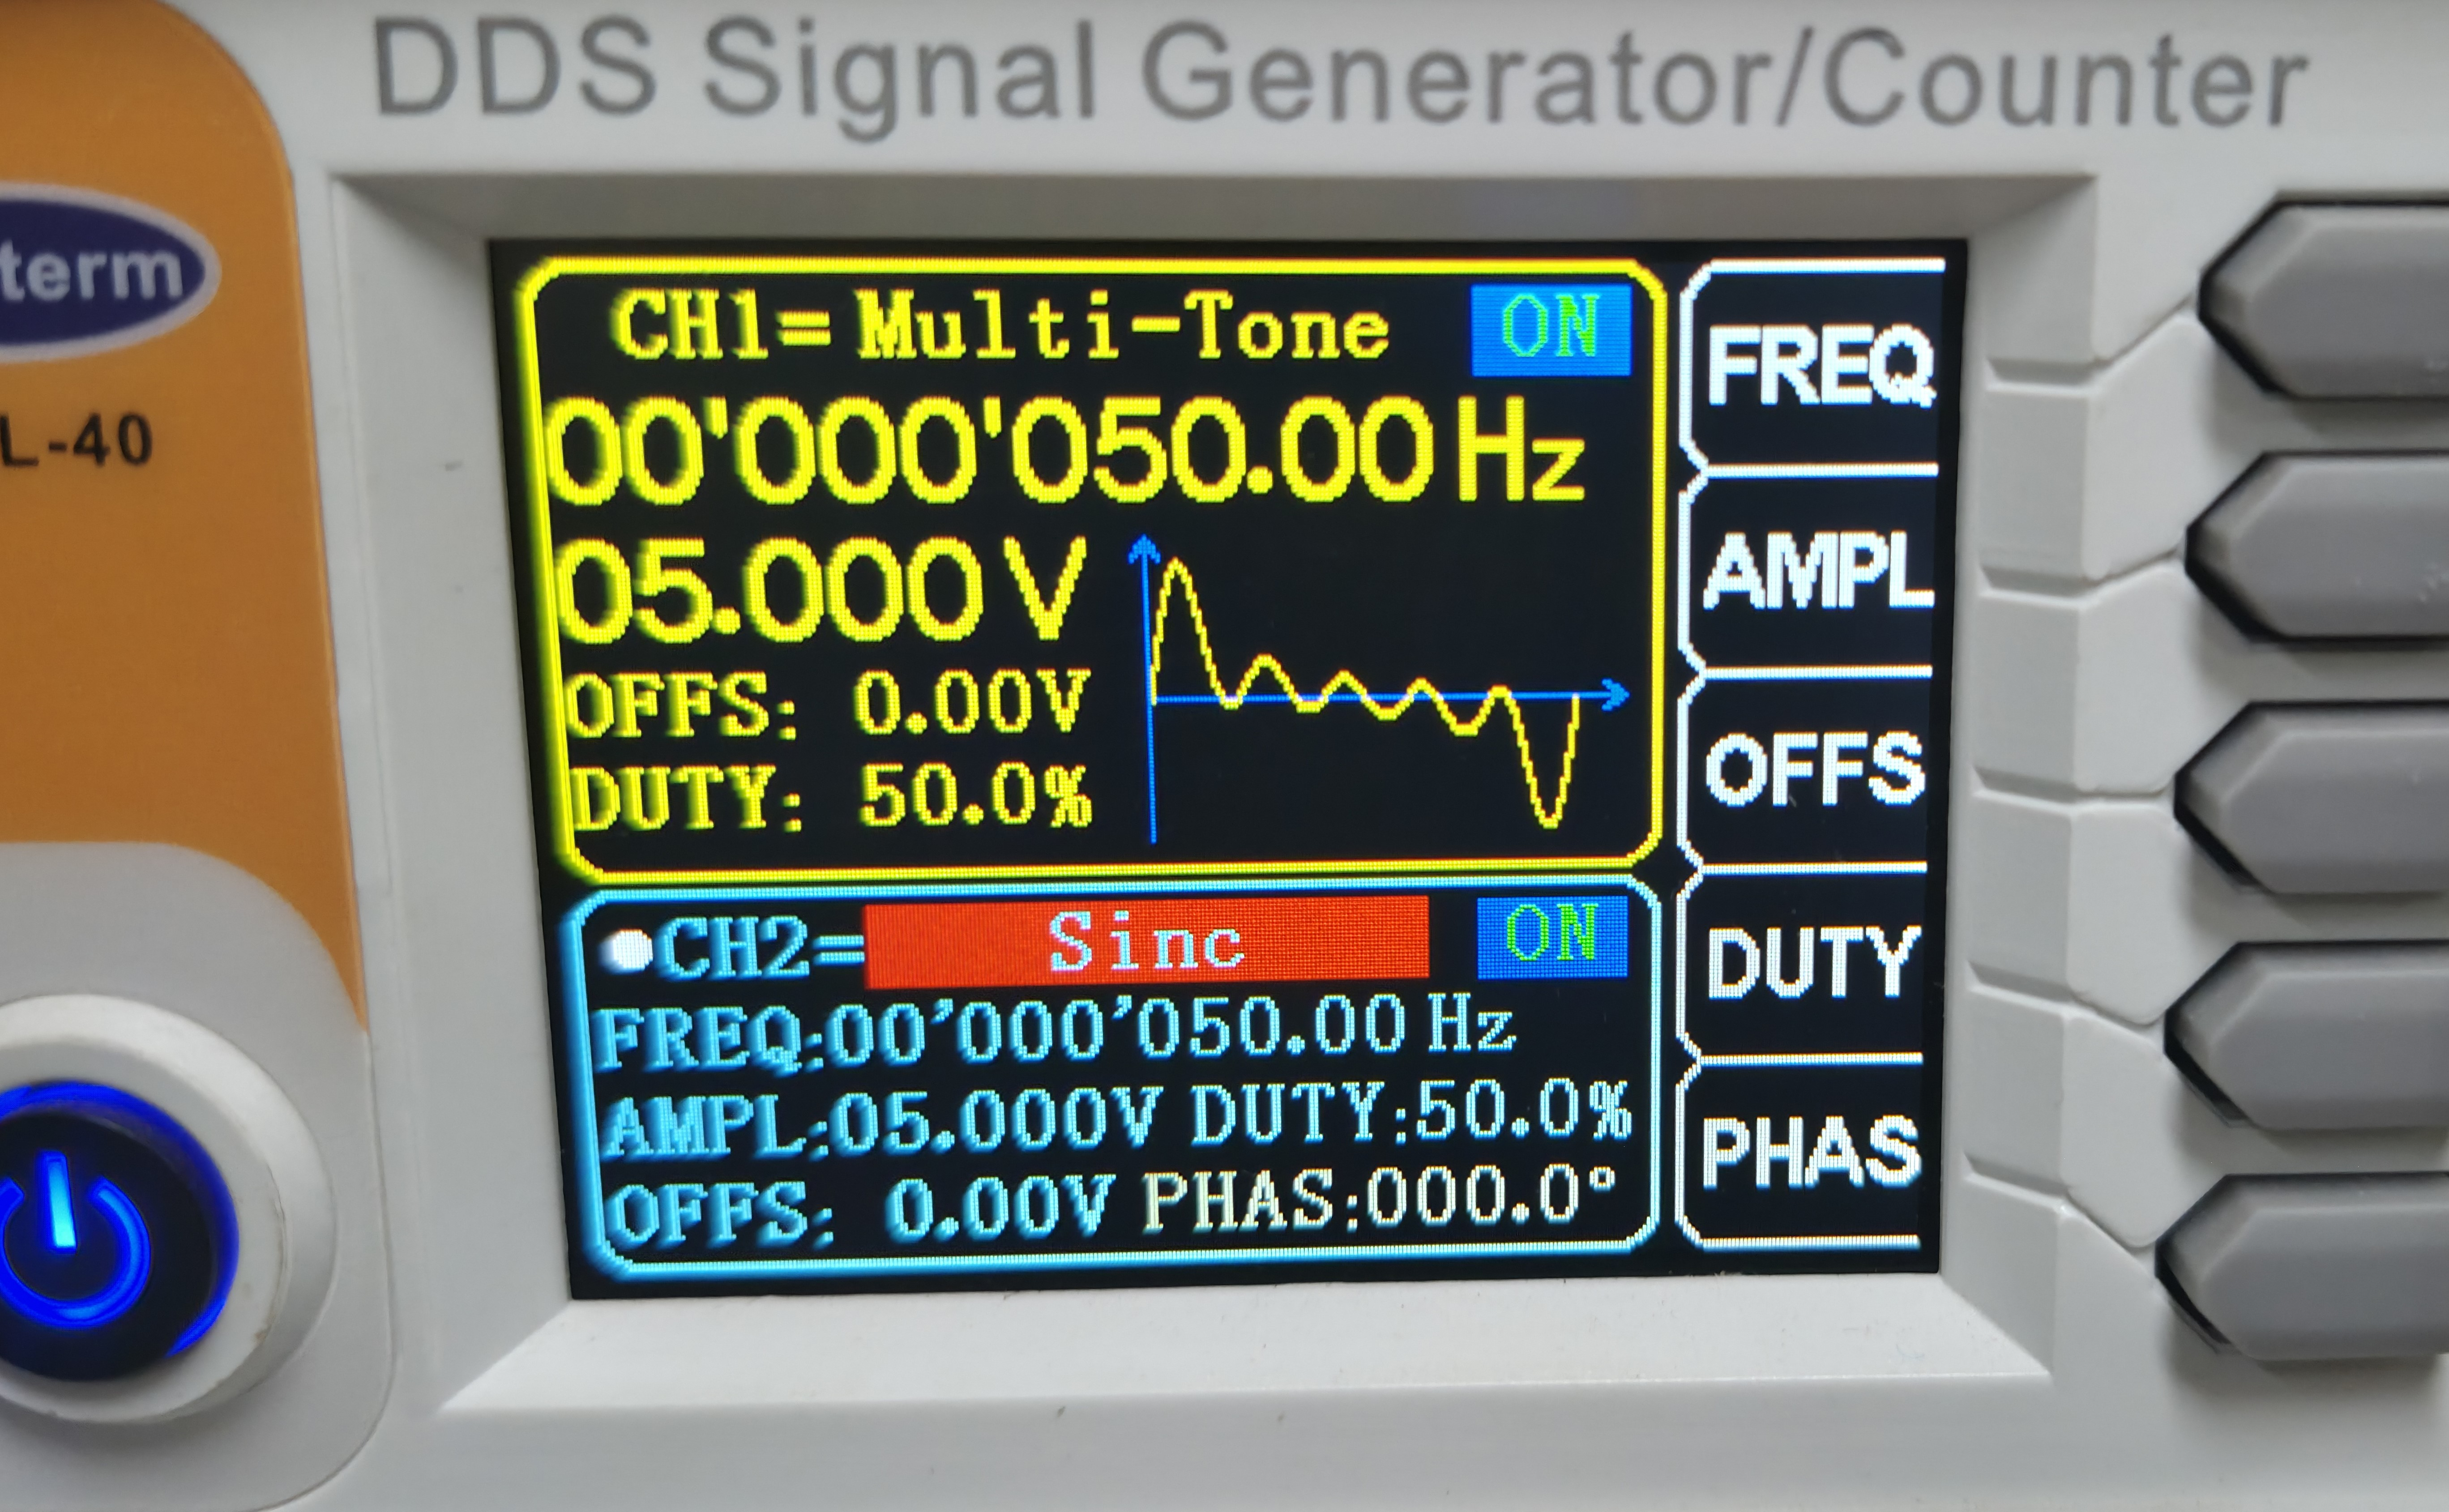
\includegraphics[width=0.82\textwidth]{figuras/configuracao_gerador_multitom_sinc.jpg}

    \caption[Configuração do gerador para sinais multitom e sinc]{
        Configuração do gerador de sinais Politerm POL-40 para a geração simultânea de um sinal multitom no canal CH1 e de um sinal sinc no canal CH2. Ambos os canais foram habilitados com frequência ajustada para 50~Hz, amplitude de 5~V, deslocamento contínuo nulo e razão cíclica de 50\%. Para o sinal sinc do canal CH2, a fase foi ajustada para $0^\circ$.
    }

    \label{fig:configuracao_gerador_multitom_sinc}
\end{figure}

A Figura~\ref{fig:osciloscopio_multitom_sinc} apresenta a visualização simultânea dos dois sinais no osciloscópio. A forma multitom é mostrada no primeiro canal, enquanto o sinal sinc é apresentado no segundo. As leituras automáticas de frequência do osciloscópio para o sinal multitom variaram conforme a configuração de medição, pois a forma composta apresenta múltiplos cruzamentos por zero e diferentes máximos locais em cada período.

\begin{figure}[!htbp]
    \centering

    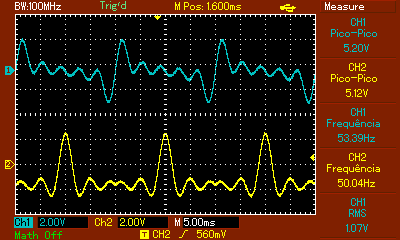
\includegraphics[width=0.68\textwidth]{figuras/osciloscopio_multitom_sinc.png}

    \caption[Visualização dos sinais multitom e sinc no osciloscópio]{
        Visualização simultânea, no osciloscópio de referência, do sinal multitom aplicado ao canal CH1, representado em ciano, e do sinal sinc aplicado ao canal CH2, representado em amarelo. As medições automáticas indicaram frequências de 50,39~Hz e 50,04~Hz e tensões de pico a pico de 5,20~V e 5,12~V para os canais CH1 e CH2, respectivamente. Ambos os canais foram exibidos com escala vertical de 2~V por divisão e base de tempo de 5~ms por divisão.
    }

    \label{fig:osciloscopio_multitom_sinc}
\end{figure}

\subsubsection{Resultados no domínio do tempo}
\label{subsubsec:multitom_tempo}

A forma de onda adquirida apresentou valores mínimo e máximo de $-2,5175$~V e 2,5672~V, respectivamente, resultando em uma amplitude pico a pico de 5,0847~V. O valor médio foi de 61,75~mV e o valor eficaz total foi de 1,0164~V. Em relação à amplitude de 5~V configurada no gerador, a amplitude pico a pico adquirida apresentou diferença de 1,69\%.

A frequência-base estimada foi de 49,9981~Hz, correspondente a um período de repetição de 20,0007~ms. O erro relativo em relação aos 50~Hz configurados foi de $-0,00371$\%. Embora o sinal possua componentes até 250~Hz, a repetição de sua forma composta ocorre a cada período da componente fundamental de 50~Hz.

A Figura~\ref{fig:multitom_tempo} apresenta um trecho contendo três períodos da forma de onda. O traçado evidencia a combinação das cinco componentes senoidais, produzindo regiões de interferência construtiva, nas quais a amplitude se aproxima dos valores extremos, e regiões de interferência destrutiva, nas quais o sinal permanece próximo de zero.

\begin{figure}[!htbp]
    \centering

    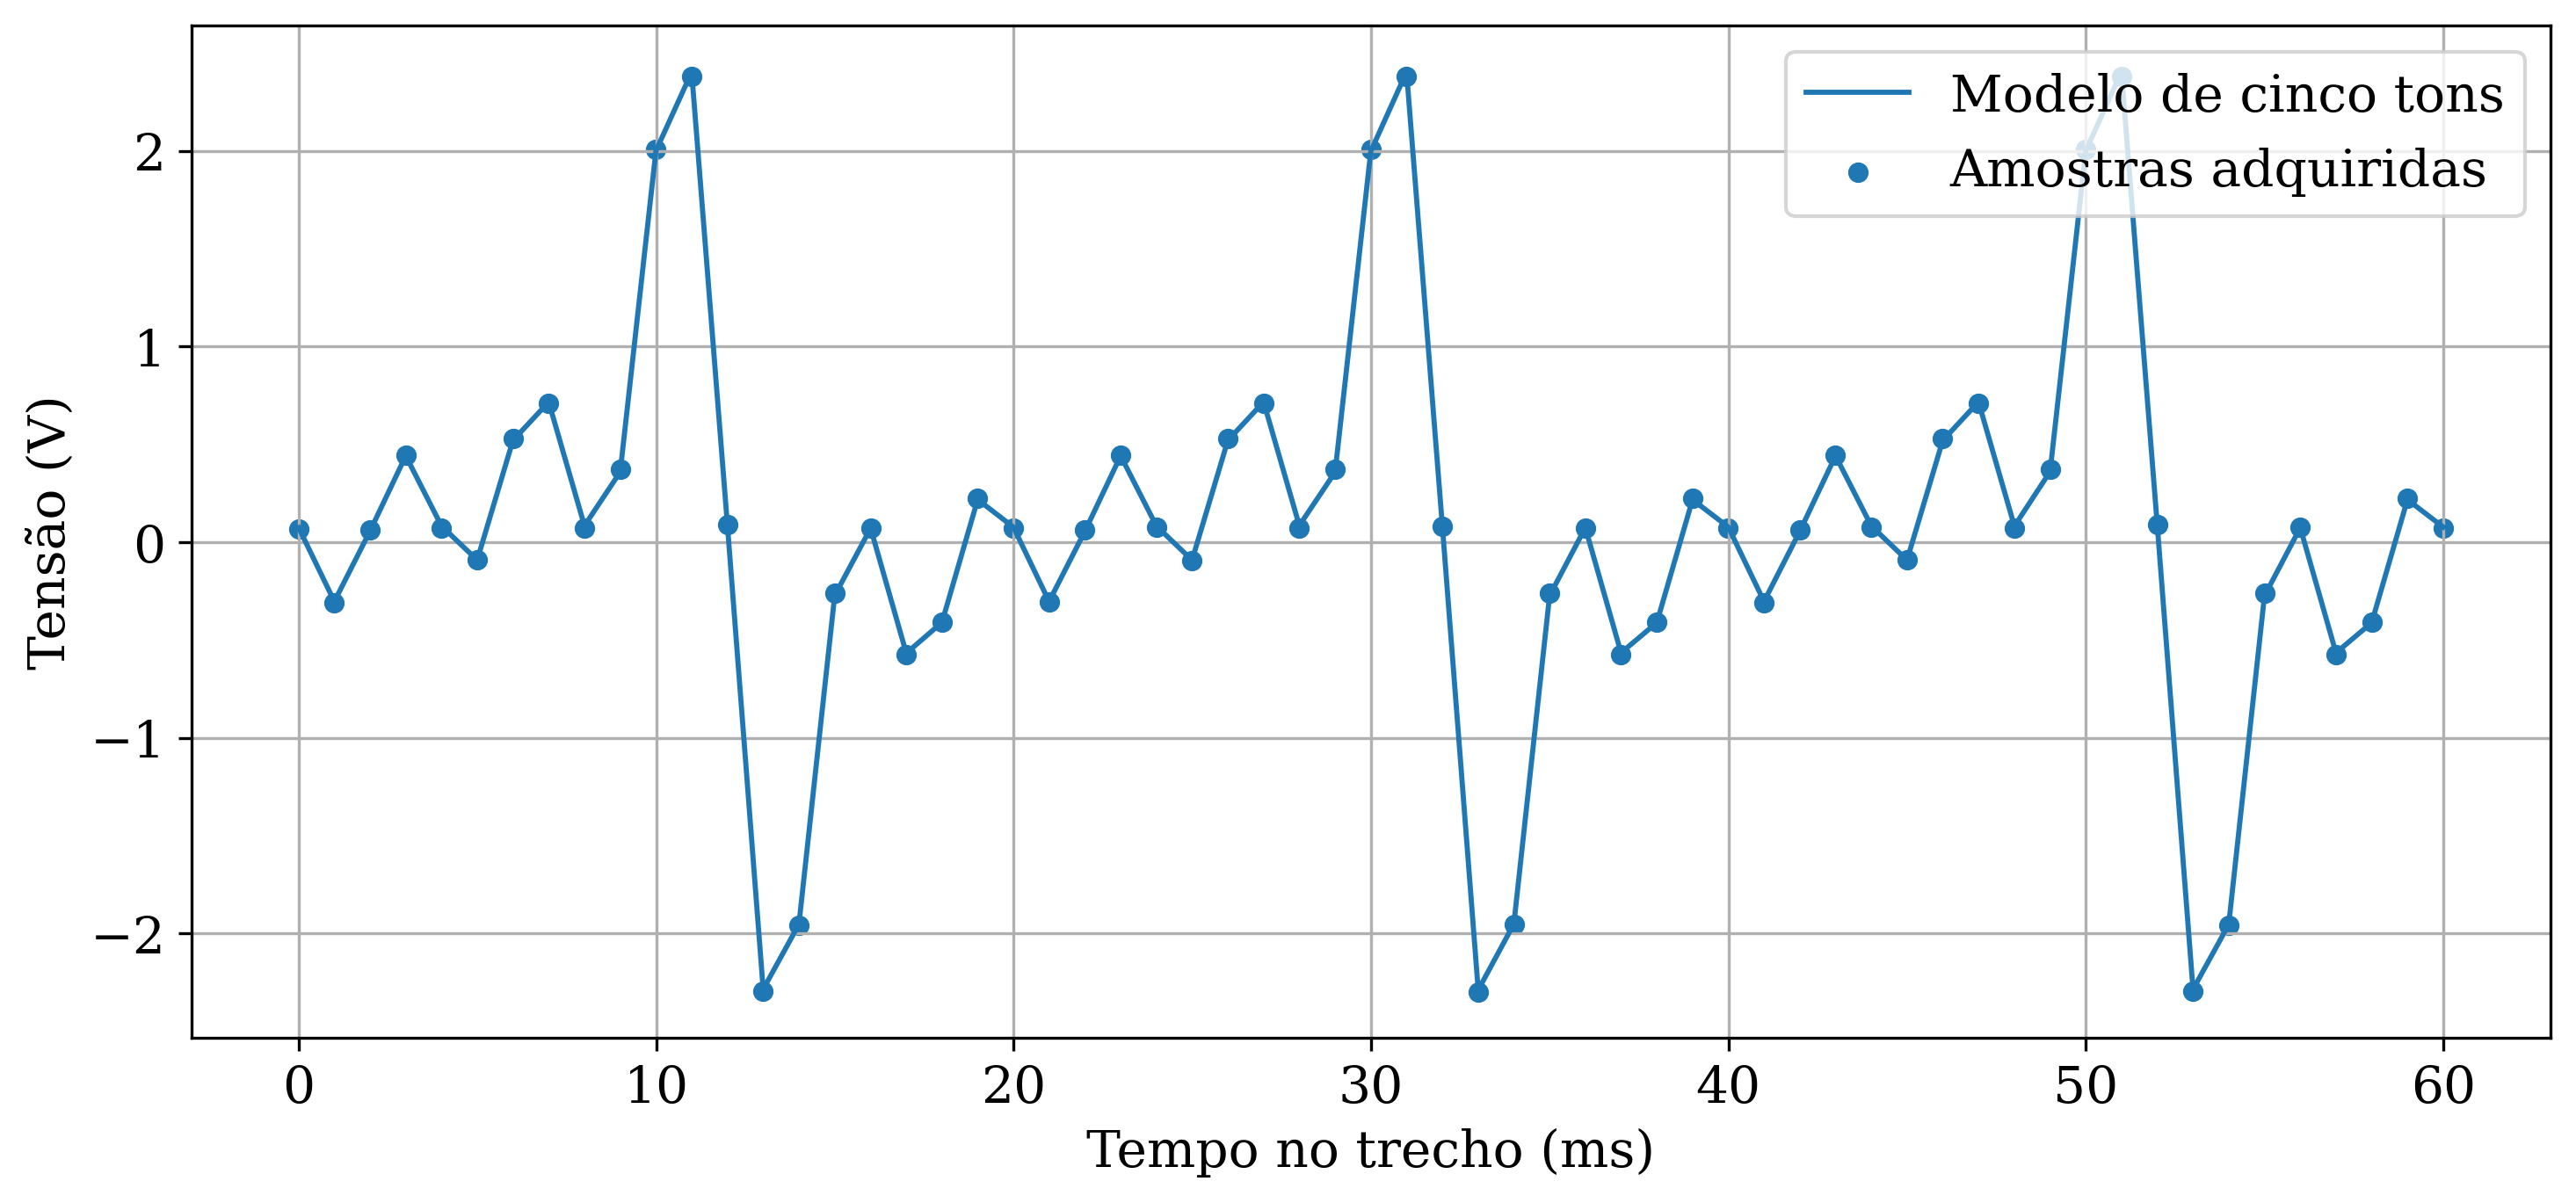
\includegraphics[width=\textwidth]{figuras/figura_multitom_tempo.png}

    \caption[Sinal multitom adquirido e modelo de cinco tons]{
        Representação, no domínio do tempo, do sinal multitom adquirido durante um intervalo de 60~ms e do modelo ajustado pela soma de cinco componentes senoidais. Os marcadores representam as amostras de tensão adquiridas, enquanto a linha contínua corresponde ao modelo de cinco tons. A sobreposição entre os dados experimentais e o modelo evidencia a concordância do ajuste com a forma de onda medida e sua repetição aproximadamente periódica ao longo do trecho analisado.
    }

    \label{fig:multitom_tempo}
\end{figure}

O ajuste realizado com as cinco componentes esperadas apresentou coeficiente de determinação de 0,99989 e erro quadrático médio normalizado de 1,0513\%. Esses valores indicam que a maior parte da variação temporal do sinal adquirido foi explicada pelas componentes de 50, 100, 150, 200 e 250~Hz.

Na medição detalhada do osciloscópio, foram observados valor máximo de 2,56~V, valor mínimo de $-2,64$~V, amplitude pico a pico de 5,20~V e valor eficaz de 1,07~V. O valor máximo obtido pelo sistema diferiu em aproximadamente 0,28\% da referência, enquanto o valor mínimo apresentou diferença de aproximadamente 4,64\% em módulo. A amplitude pico a pico adquirida foi 2,22\% inferior à medida pelo osciloscópio, e o valor eficaz foi aproximadamente 5,01\% inferior.

As frequências automáticas apresentadas pelo osciloscópio foram de 53,39~Hz na tela de visão geral e de 46,67~Hz na tela detalhada. Essa variação decorreu do algoritmo de medição automática aplicado a uma forma de onda com múltiplos picos e cruzamentos por nível em cada período. Por esse motivo, a frequência-base do sinal multitom foi determinada principalmente pela separação entre suas componentes espectrais e pelo ajuste do modelo de cinco tons, e não pela leitura automática de frequência do osciloscópio.

\begin{figure}[!htbp]
    \centering

    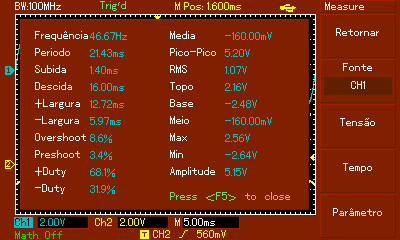
\includegraphics[width=0.68\textwidth]{figuras/osciloscopio_multitom_detalhado.png}

    \caption[Medições automáticas do sinal multitom]{
        Medições automáticas fornecidas pelo osciloscópio de referência para o sinal multitom aplicado ao canal CH1. O instrumento indicou frequência de 46,67~Hz, período de 21,43~ms, tensão de pico a pico de 5,20~V, valor eficaz de 1,07~V e amplitude de 5,15~V, com níveis superior e inferior estimados em 2,61~V e $-2,48$~V, respectivamente. A tela também apresenta razão cíclica positiva de 68,1\% e negativa de 31,9\%. Como o sinal resulta da composição de cinco componentes senoidais e não possui forma senoidal ou quadrada simples, as medições de frequência, período e razão cíclica dependem do algoritmo de detecção empregado pelo osciloscópio e não representam individualmente as frequências dos tons que compõem o sinal.
    }

    \label{fig:osciloscopio_multitom_detalhado}
\end{figure}

\subsubsection{Resultados no domínio da frequência}
\label{subsubsec:multitom_frequencia}

A análise no domínio da frequência identificou cinco componentes principais próximas das frequências esperadas de 50, 100, 150, 200 e 250~Hz. As frequências ajustadas foram de 49,9981, 99,9963, 149,9944, 199,9926 e 249,9907~Hz, respectivamente. Todas apresentaram erro relativo de aproximadamente $-0,00371$\%, compatível com a diferença entre a taxa efetiva e a taxa nominal utilizada na análise.

A Figura~\ref{fig:multitom_espectro} apresenta o espectro adquirido e as amplitudes obtidas pelo ajuste das cinco componentes. Os picos permaneceram claramente separados, com espaçamento de aproximadamente 50~Hz, sem sobreposição relevante entre os lóbulos espectrais associados a cada tom.

\begin{figure}[!htbp]
    \centering

    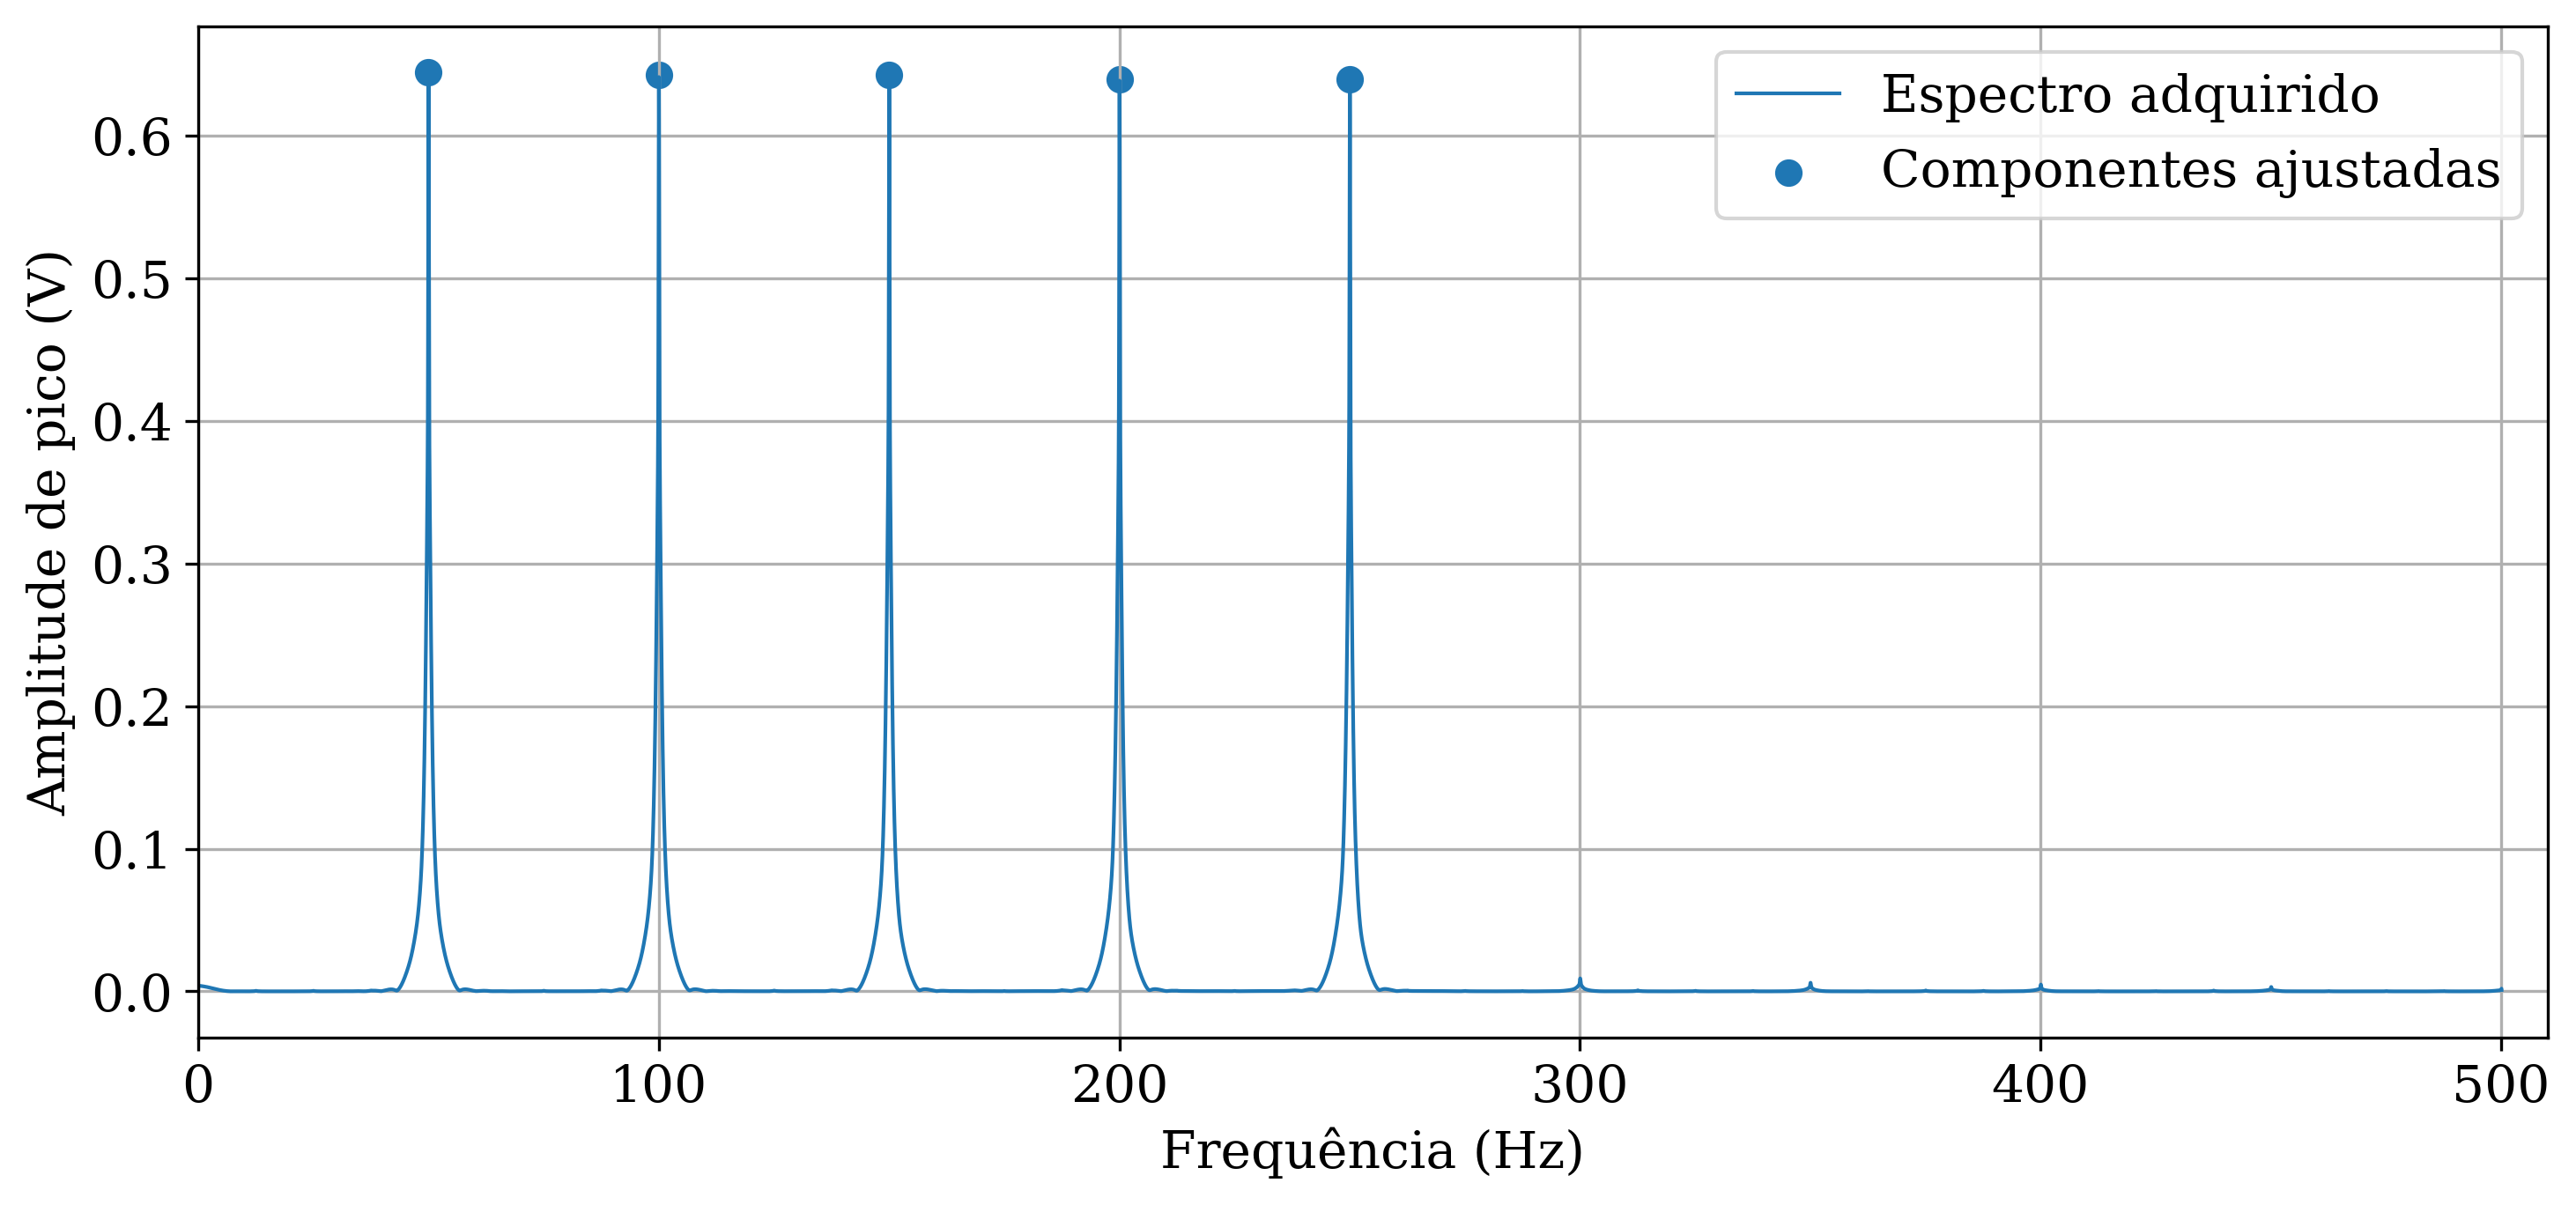
\includegraphics[width=\textwidth]{figuras/figura_multitom_espectro.png}

    \caption[Espectro do sinal multitom e componentes ajustadas]{
        Espectro em amplitude de pico do sinal multitom adquirido, com cinco componentes principais aproximadamente equiespaçadas em 50, 100, 150, 200 e 250~Hz. A linha contínua representa o espectro calculado a partir das amostras, enquanto os marcadores indicam as frequências e amplitudes estimadas pelo modelo de cinco tons. As componentes apresentam amplitudes próximas de 0,64~V, e a coincidência dos marcadores com os respectivos picos espectrais evidencia a concordância entre o modelo ajustado e o sinal medido. As componentes de menor amplitude observadas acima de 250~Hz correspondem a resíduos presentes no espectro adquirido.
    }

    \label{fig:multitom_espectro}
\end{figure}

As amplitudes de pico ajustadas foram de 0,6445~V para 50~Hz, 0,6425~V para 100~Hz, 0,6424~V para 150~Hz, 0,6395~V para 200~Hz e 0,6394~V para 250~Hz. Tomando a componente de 50~Hz como referência, as demais apresentaram níveis relativos de $-0,0274$, $-0,0290$, $-0,0686$ e $-0,0700$~dBc.

A diferença entre a maior e a menor amplitude foi de apenas 0,0700~dB. Esse resultado demonstra que as cinco componentes foram adquiridas com amplitudes praticamente uniformes, conforme esperado para a configuração multitom utilizada.

\begin{figure}[!htbp]
    \centering
    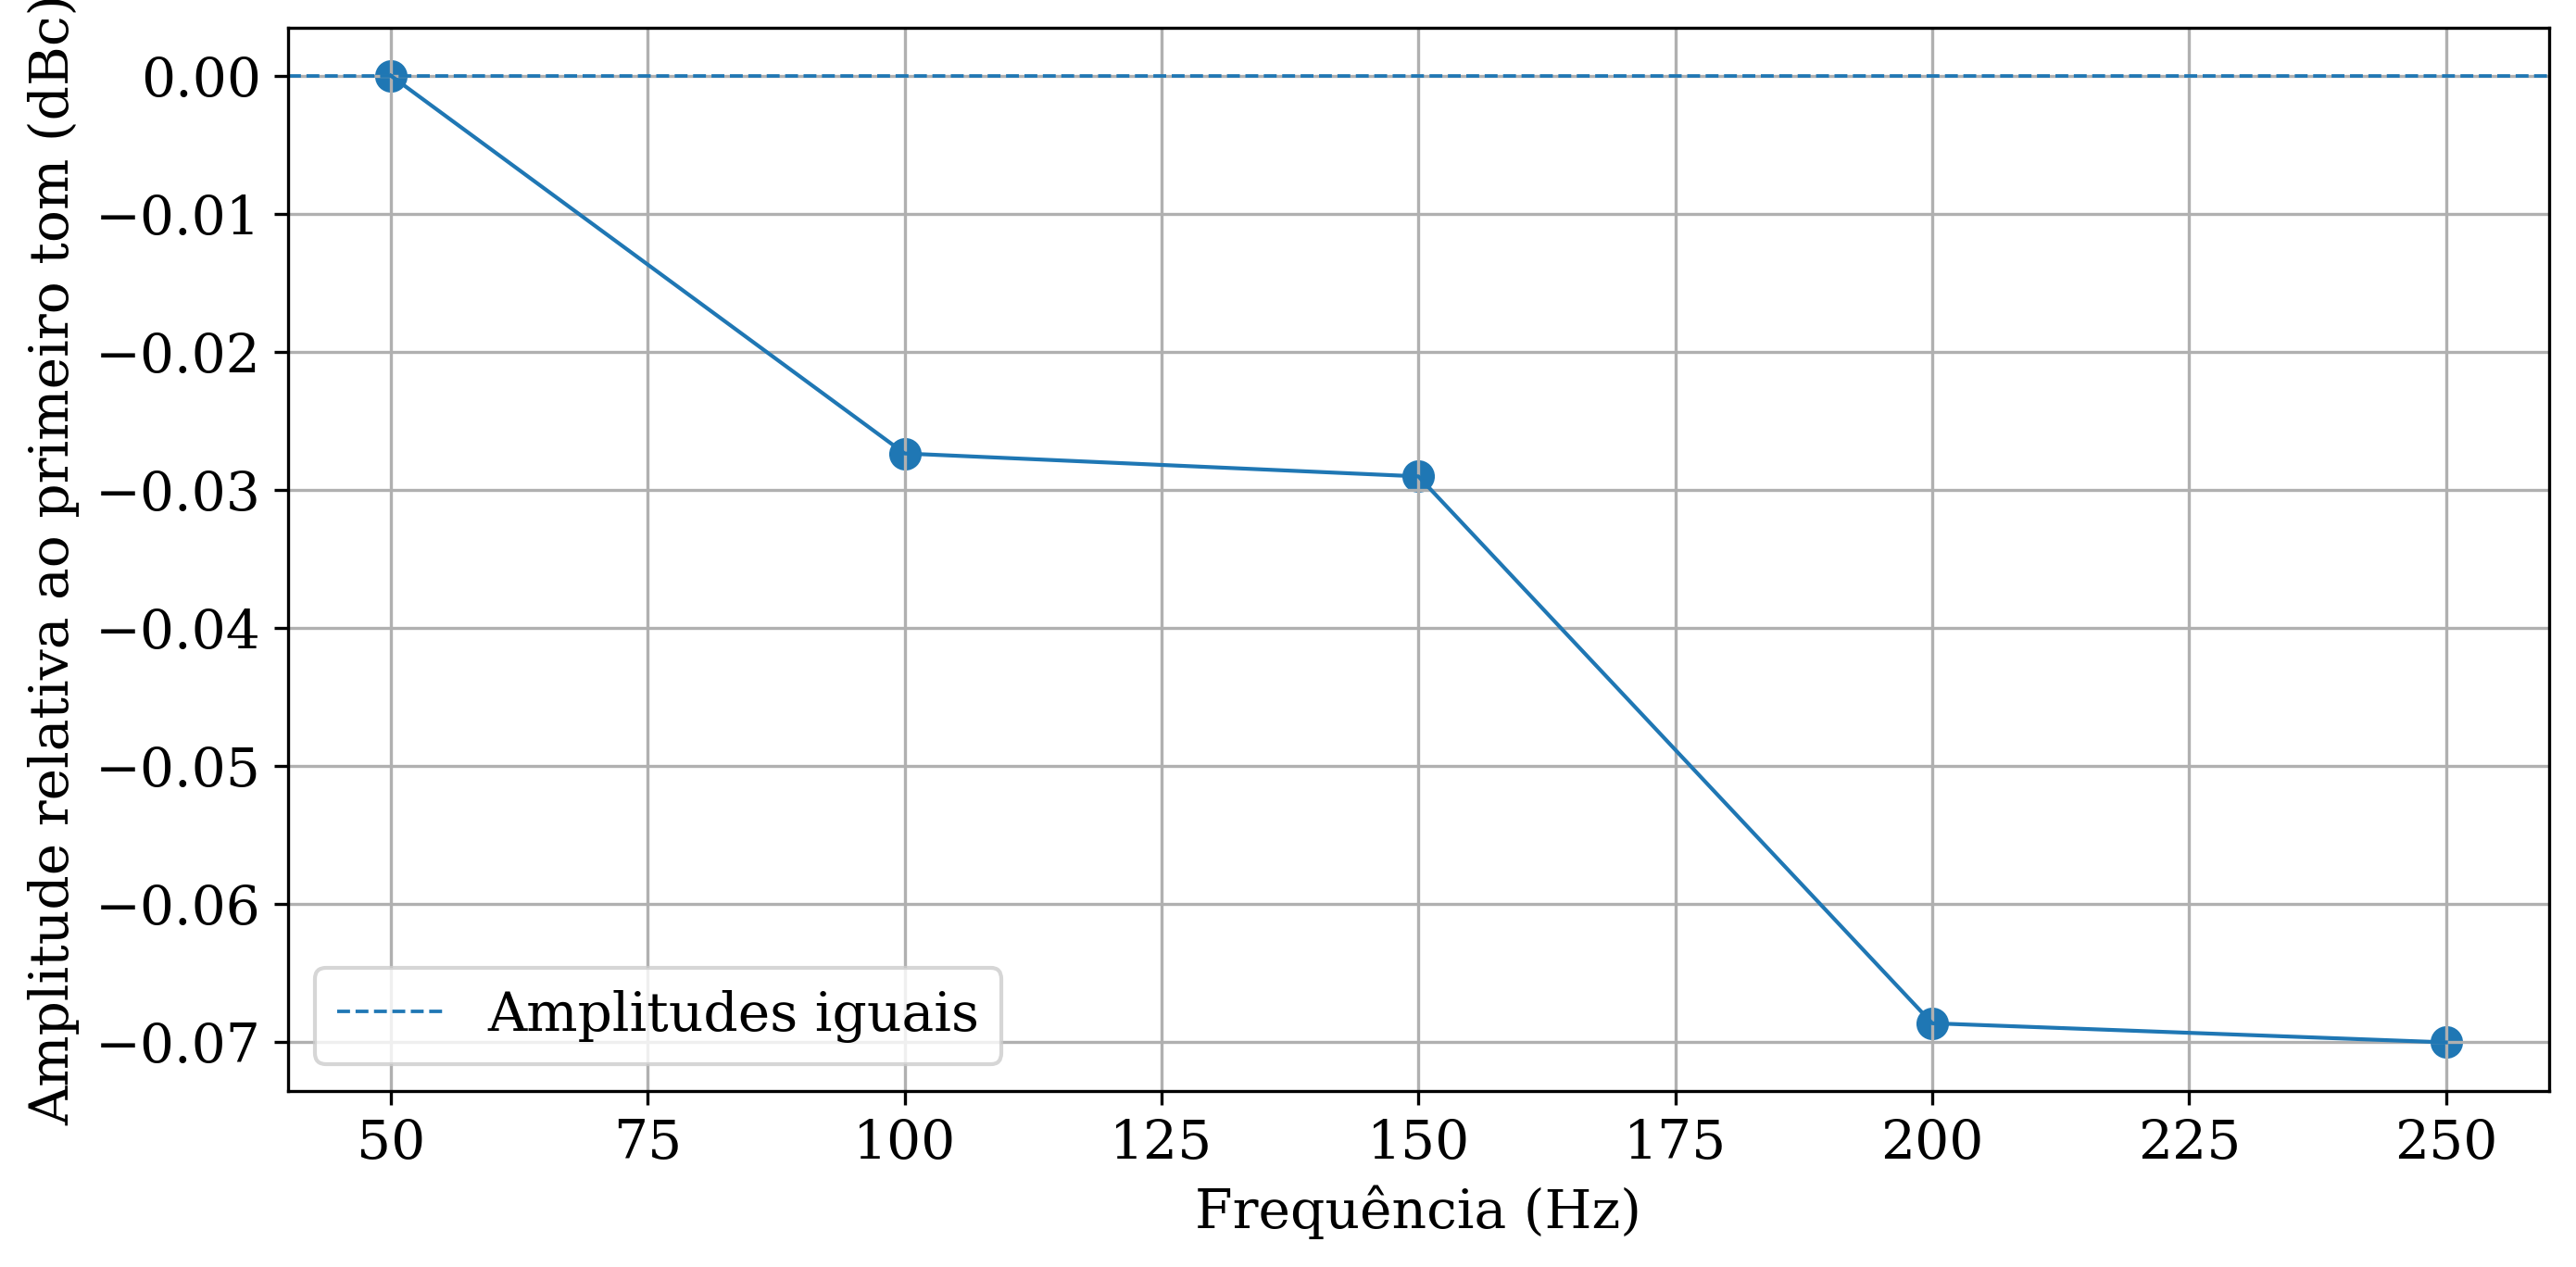
\includegraphics[width=\textwidth]{figuras/figura_multitom_componentes_relativas.png}
    \caption[Amplitude relativa das componentes do sinal multitom]
    {Amplitude relativa das cinco componentes do sinal multitom, localizadas em 50, 100, 150, 200 e 250~Hz, expressa em relação ao primeiro tom, de 50~Hz, definido como 0~dBc. A linha tracejada em 0~dBc representa a condição ideal de amplitudes iguais. As diferenças observadas são inferiores a 0,07~dB, indicando elevada uniformidade entre as amplitudes das componentes.}
    \label{fig:multitom_componentes_relativas}
\end{figure}

A Tabela~\ref{tab:componentes_multitom} sintetiza as frequências e amplitudes obtidas para cada componente.

\begin{table}[!htbp]
    \centering
    \caption{Componentes principais identificadas no sinal multitom.}
    \label{tab:componentes_multitom}
    \small
        \begin{tabular}{c c c c c c}
            \hline
            \textbf{Componente} &
            \textbf{1} &
            \textbf{2} &
            \textbf{3} &
            \textbf{4} &
            \textbf{5} \\
            \hline
            \textbf{Frequência esperada (Hz)}
            & 50 & 100 & 150 & 200 & 250 \\

            \textbf{Frequência ajustada (Hz)}
            & 49,9981 & 99,9963 & 149,9944 & 199,9926 & 249,9907 \\

            \textbf{Erro relativo (\%)}
            & $-0,00371$ & $-0,00371$ & $-0,00371$
            & $-0,00371$ & $-0,00371$ \\

            \textbf{Amplitude de pico (V)}
            & 0,6445 & 0,6425 & 0,6424 & 0,6395 & 0,6394 \\

            \textbf{Amplitude relativa (dBc)}
            & 0,0000 & $-0,0274$ & $-0,0290$ & $-0,0686$ & $-0,0700$ \\
            \hline
        \end{tabular}

\end{table}



Após a remoção das cinco componentes principais do modelo, a maior componente residual foi encontrada em aproximadamente 300,04~Hz, com amplitude de pico de 9,64~mV e nível relativo de $-36,50$~dBc. Outras componentes foram observadas próximas de 350,05, 400,06, 450,07 e 500,07~Hz, com níveis progressivamente menores, entre aproximadamente $-40,10$ e $-48,44$~dBc.

A componente próxima de 60~Hz apresentou nível de aproximadamente $-66,54$~dBc, permanecendo significativamente abaixo dos cinco tons principais. A faixa dinâmica entre os tons modelados e a maior componente residual foi de aproximadamente 36,50~dB.

\subsubsection{Discussão dos resultados}
\label{subsubsec:discussao_multitom}

Os resultados demonstraram que a plataforma foi capaz de adquirir simultaneamente cinco componentes espectrais distintas e preservar sua separação no domínio da frequência. Os erros relativos das frequências permaneceram inferiores a 0,004\%, enquanto a diferença máxima entre as amplitudes dos tons foi inferior a 0,1~dB.

A elevada correspondência entre o sinal adquirido e o modelo de cinco tons também foi observada no domínio do tempo, no qual o coeficiente de determinação foi superior a 0,9998. A forma composta, incluindo seus máximos, mínimos e regiões de cancelamento parcial, foi preservada ao longo dos períodos analisados.

As componentes residuais acima de 250~Hz apresentaram amplitudes pelo menos 36,5~dB inferiores às componentes principais. Sua presença pode estar relacionada ao conteúdo adicional produzido pelo gerador, às não linearidades da cadeia de aquisição, ao vazamento espectral residual ou ao acoplamento com outros sinais. Entretanto, essas componentes não comprometeram a identificação dos cinco tons esperados.

A comparação com o osciloscópio apresentou maior concordância para os valores extremos e para a amplitude pico a pico do que para a frequência automática. Isso ocorreu porque a medição automática de frequência do osciloscópio não distinguiu diretamente a frequência fundamental da forma composta, enquanto a análise espectral permitiu identificar individualmente cada componente.

De forma geral, o ensaio confirmou que o sistema foi capaz de adquirir sinais compostos por múltiplas componentes, preservar suas frequências e manter pequenas diferenças relativas de amplitude ao longo da banda entre 50 e 250~Hz.

% ----------------------------------------------------------------------------
\subsection{Sinal sinc}
\label{subsec:sinal_sinc}

O sinal sinc foi produzido no segundo canal do gerador com frequência de repetição nominal de 50~Hz, amplitude pico a pico configurada em 5~V e offset nulo. Como o gerador produziu uma forma sinc periódica, sua representação no domínio da frequência ocorreu por meio de linhas discretas separadas pela frequência de repetição, distribuídas sob um envelope espectral associado à forma do pulso.

A polaridade do sinal armazenado foi invertida apenas durante a apresentação e o ajuste, com o objetivo de alinhar sua orientação àquela mostrada pelo osciloscópio. Essa alteração correspondeu à multiplicação dos valores por $-1$ e não modificou a amplitude pico a pico, o valor eficaz, a largura temporal ou as amplitudes relativas das componentes espectrais.

\subsubsection{Resultados no domínio do tempo}
\label{subsubsec:sinc_tempo}

Após o alinhamento de polaridade, o sinal apresentou valores mínimo e máximo de $-2,5437$~V e 2,5251~V, respectivamente, resultando em uma amplitude pico a pico de 5,0688~V. O valor médio foi de $-1,2271$~V e o valor eficaz total foi de 1,7365~V.

A frequência de repetição estimada foi de 49,9982~Hz, correspondente a um período de 20,0007~ms e a um erro relativo de $-0,00369$\% em relação aos 50~Hz configurados. A amplitude máxima do pulso principal ajustado foi de 2,5192~V, enquanto o menor valor do ciclo médio foi de aproximadamente $-2,5351$~V.

A Figura~\ref{fig:sinc_tempo} apresenta as amostras adquiridas ao longo de um período e o modelo periódico ajustado. O pulso principal foi observado próximo do centro do ciclo, acompanhado de oscilações laterais de menor amplitude distribuídas antes e depois do máximo.

\begin{figure}[!htbp]
    \centering
    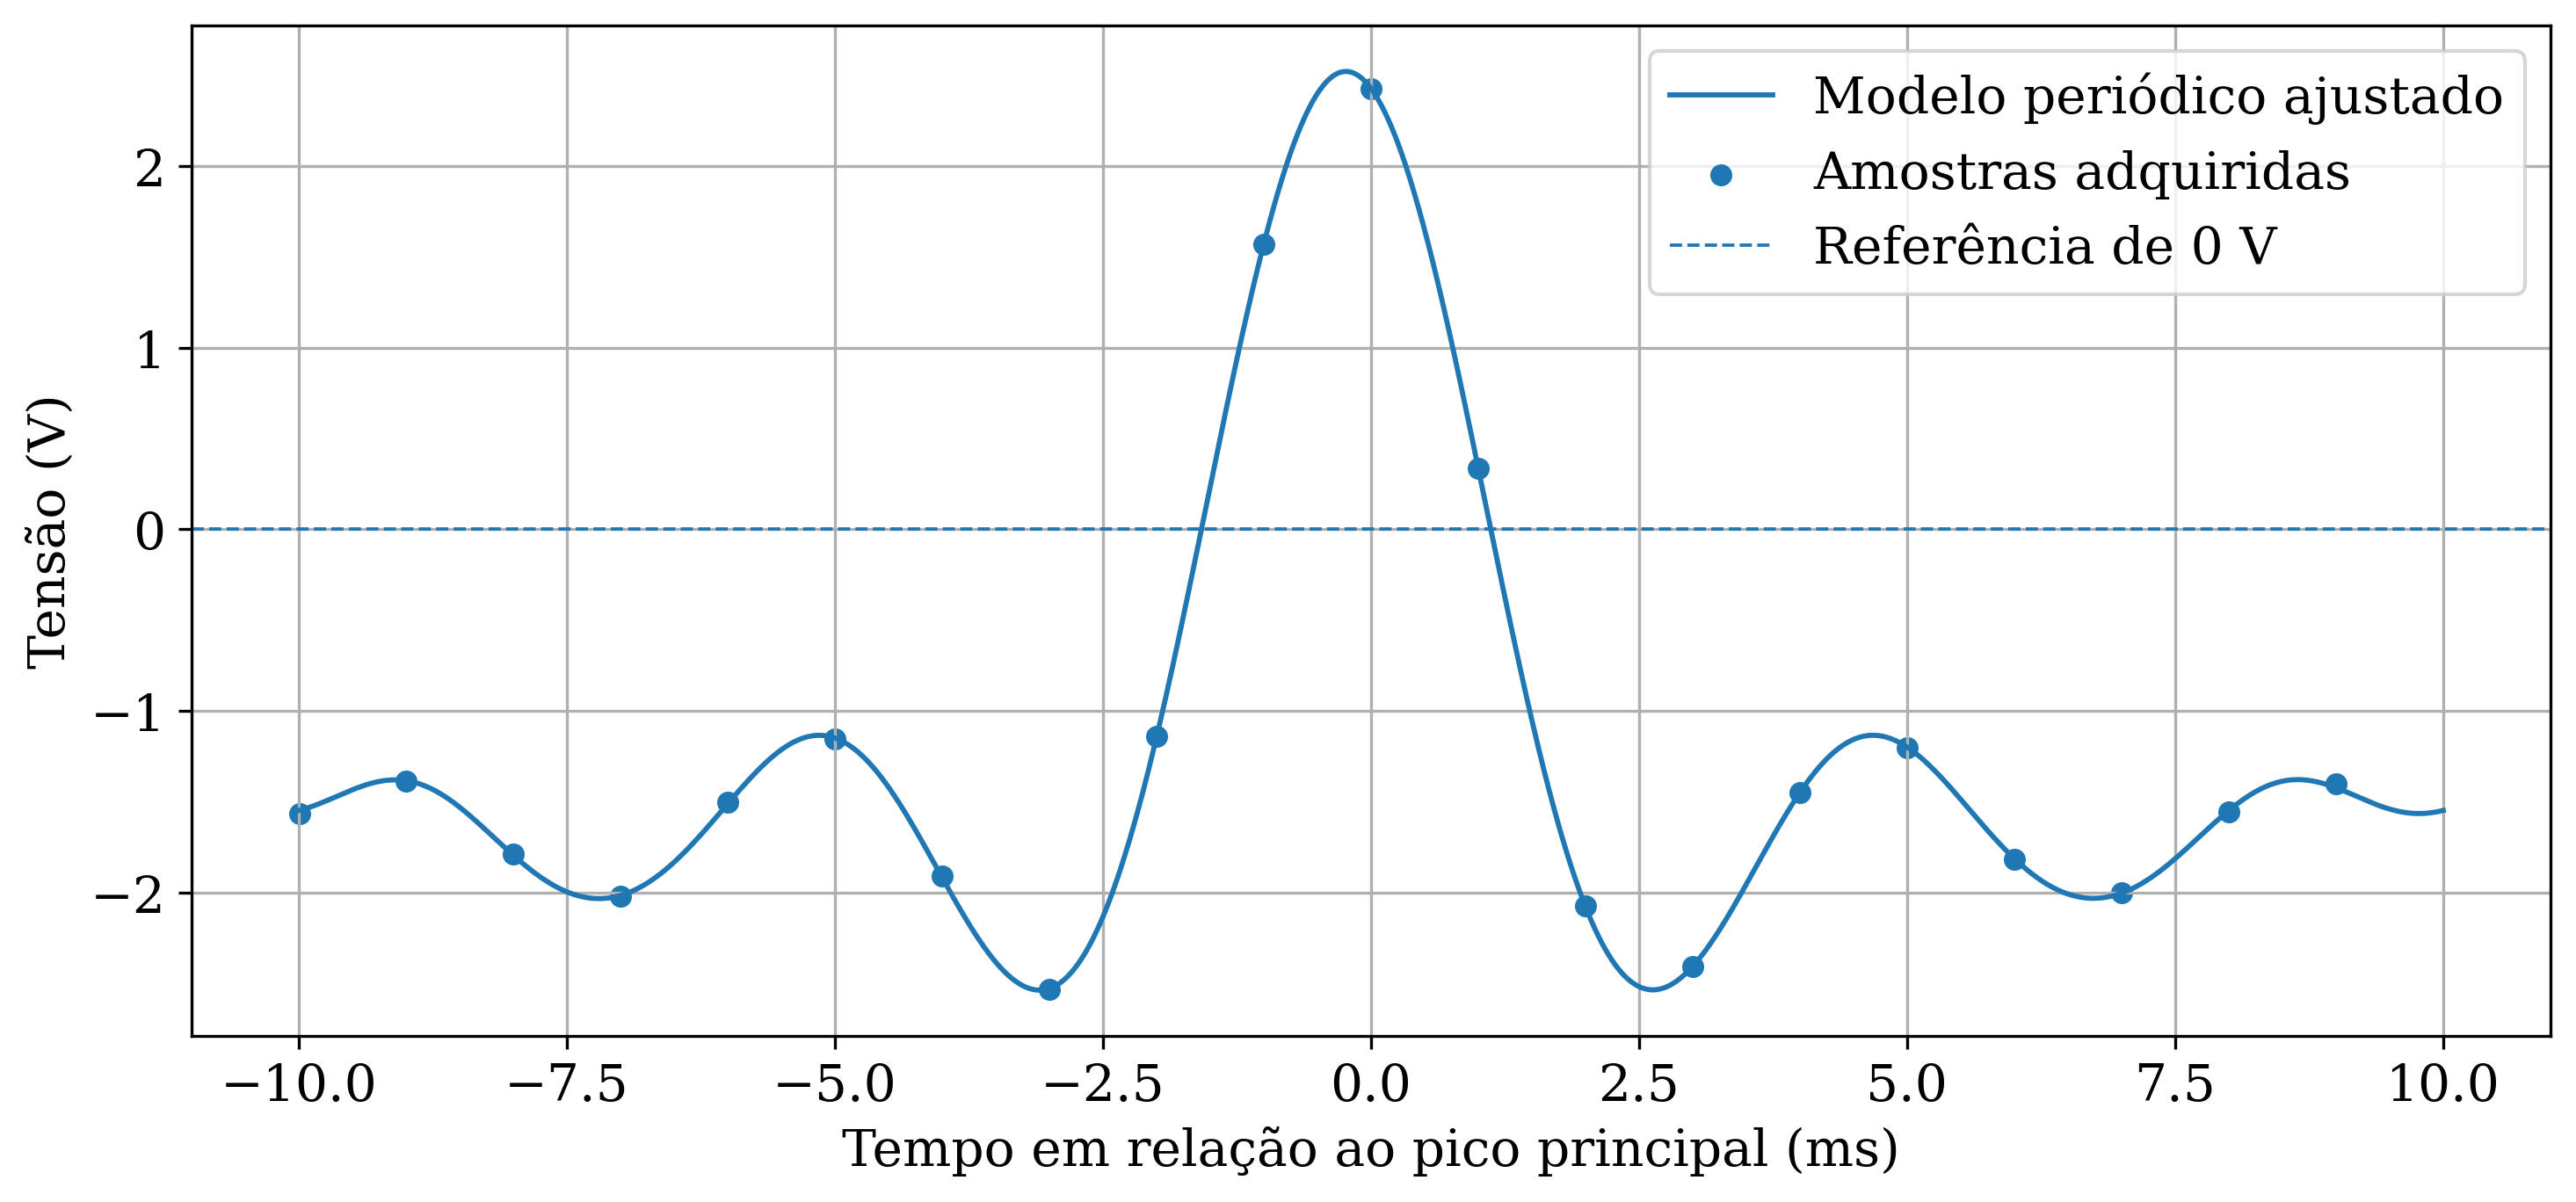
\includegraphics[width=\textwidth]{figuras/figura_sinc_tempo.png}
    \caption[Representação temporal do sinal sinc e do modelo ajustado]
    {Representação temporal, em volts, do sinal sinc adquirido no intervalo de $-10$ a $10$~ms, com o tempo expresso em relação ao pico principal. Os marcadores representam as amostras adquiridas, a linha contínua corresponde ao modelo periódico ajustado e a linha tracejada indica a referência de $0$~V.}
    \label{fig:sinc_tempo}
\end{figure}

O modelo periódico apresentou coeficiente de determinação de 0,99993 e erro quadrático médio normalizado de 0,8351\%. A elevada correspondência indica que o pulso principal e os lóbulos laterais permaneceram regulares ao longo dos ciclos considerados.

Os primeiros cruzamentos por zero em torno do pulso principal foram estimados em $-1,3481$~ms e 1,3511~ms em relação ao máximo. A largura do lóbulo principal entre esses cruzamentos foi, portanto, de 2,6992~ms. A largura medida à meia altura foi de aproximadamente 1,7906~ms.

Os primeiros mínimos laterais foram identificados em aproximadamente $-2,8577$~ms e 2,8623~ms, com amplitudes de $-2,5351$~V e $-2,5335$~V. Os máximos laterais seguintes foram observados em aproximadamente $-4,9130$~ms e 4,9150~ms, com amplitudes próximas de $-1,133$~V. A simetria entre as posições dos lóbulos à esquerda e à direita do pulso principal indica que a organização temporal da forma de onda foi preservada.

Na medição detalhada do osciloscópio, foram obtidas frequência de 49,98~Hz, amplitude pico a pico de 5,20~V, valor eficaz de 1,69~V, valor médio de $-1,28$~V, máximo de 2,56~V e mínimo de $-2,64$~V. A largura positiva informada pelo instrumento foi de aproximadamente 2,84~ms.

A frequência estimada pelo sistema diferiu em aproximadamente 0,036\% da leitura detalhada do osciloscópio. A amplitude pico a pico foi 2,52\% inferior à referência, enquanto o valor eficaz foi 2,75\% superior. O valor médio diferiu em aproximadamente 4,13\%, e os valores máximo e mínimo apresentaram diferenças de aproximadamente 1,36\% e 3,65\%, respectivamente.

A largura de 2,6992~ms calculada entre os cruzamentos por zero foi aproximadamente 4,96\% inferior à largura positiva de 2,84~ms apresentada pelo osciloscópio. Essa comparação deve ser interpretada com cautela, pois o sistema utilizou diretamente os cruzamentos interpolados por 0~V, enquanto a largura automática do osciloscópio foi determinada pelo algoritmo interno do instrumento.

\begin{figure}[!htbp]
    \centering
    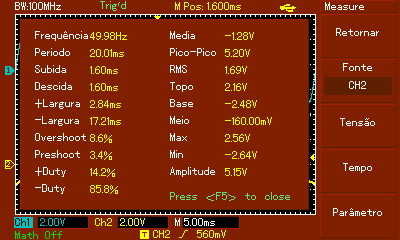
\includegraphics[width=0.68\textwidth]{figuras/osciloscopio_sinc_detalhado.png}
    \caption[Medições automáticas do sinal sinc no osciloscópio]
    {Painel de medições automáticas do osciloscópio para o sinal sinc adquirido no canal CH2. Foram obtidos frequência de 49,98~Hz, período de 20,01~ms, tensão pico a pico de 5,20~V, valor eficaz de 1,69~V e valor médio de $-1,28$~V. Os valores máximo e mínimo medidos foram, respectivamente, 2,56~V e $-2,64$~V, enquanto os tempos de subida e de descida foram ambos de 1,60~ms.}
    \label{fig:osciloscopio_sinc_detalhado}
\end{figure}

\begin{table}[!htbp]
    \centering
    \caption{Comparação das principais métricas temporais do sinal sinc.}
    \label{tab:comparacao_sinc_osciloscopio}
    \small
    \begin{tabular}{p{5.5cm} c c}
        \hline
        \textbf{Métrica} &
        \textbf{Sistema desenvolvido} &
        \textbf{Osciloscópio} \\
        \hline
        Frequência de repetição & 49,9982~Hz & 49,98~Hz \\
        Amplitude pico a pico & 5,0688~V & 5,20~V \\
        Valor eficaz & 1,7365~V & 1,69~V \\
        Valor médio & $-1,2271$~V & $-1,28$~V \\
        Valor máximo & 2,5251~V & 2,56~V \\
        Valor mínimo & $-2,5437$~V & $-2,64$~V \\
        Largura do pulso & 2,6992~ms & 2,84~ms \\
        \hline
    \end{tabular}
\end{table}

\subsubsection{Resultados no domínio da frequência}
\label{subsubsec:sinc_frequencia}

Por se tratar de uma forma sinc repetida periodicamente a aproximadamente 50~Hz, o espectro adquirido foi constituído por linhas discretas separadas por aproximadamente 49,9982~Hz. As componentes foram observadas próximas de 50, 100, 150, 200, 250, 300, 350, 400, 450 e 500~Hz.

A Figura~\ref{fig:sinc_espectro} apresenta o espectro em escala linear. As maiores componentes foram encontradas entre 50 e 200~Hz, enquanto uma redução acentuada ocorreu a partir da componente de 250~Hz.

\begin{figure}[!htbp]
    \centering
    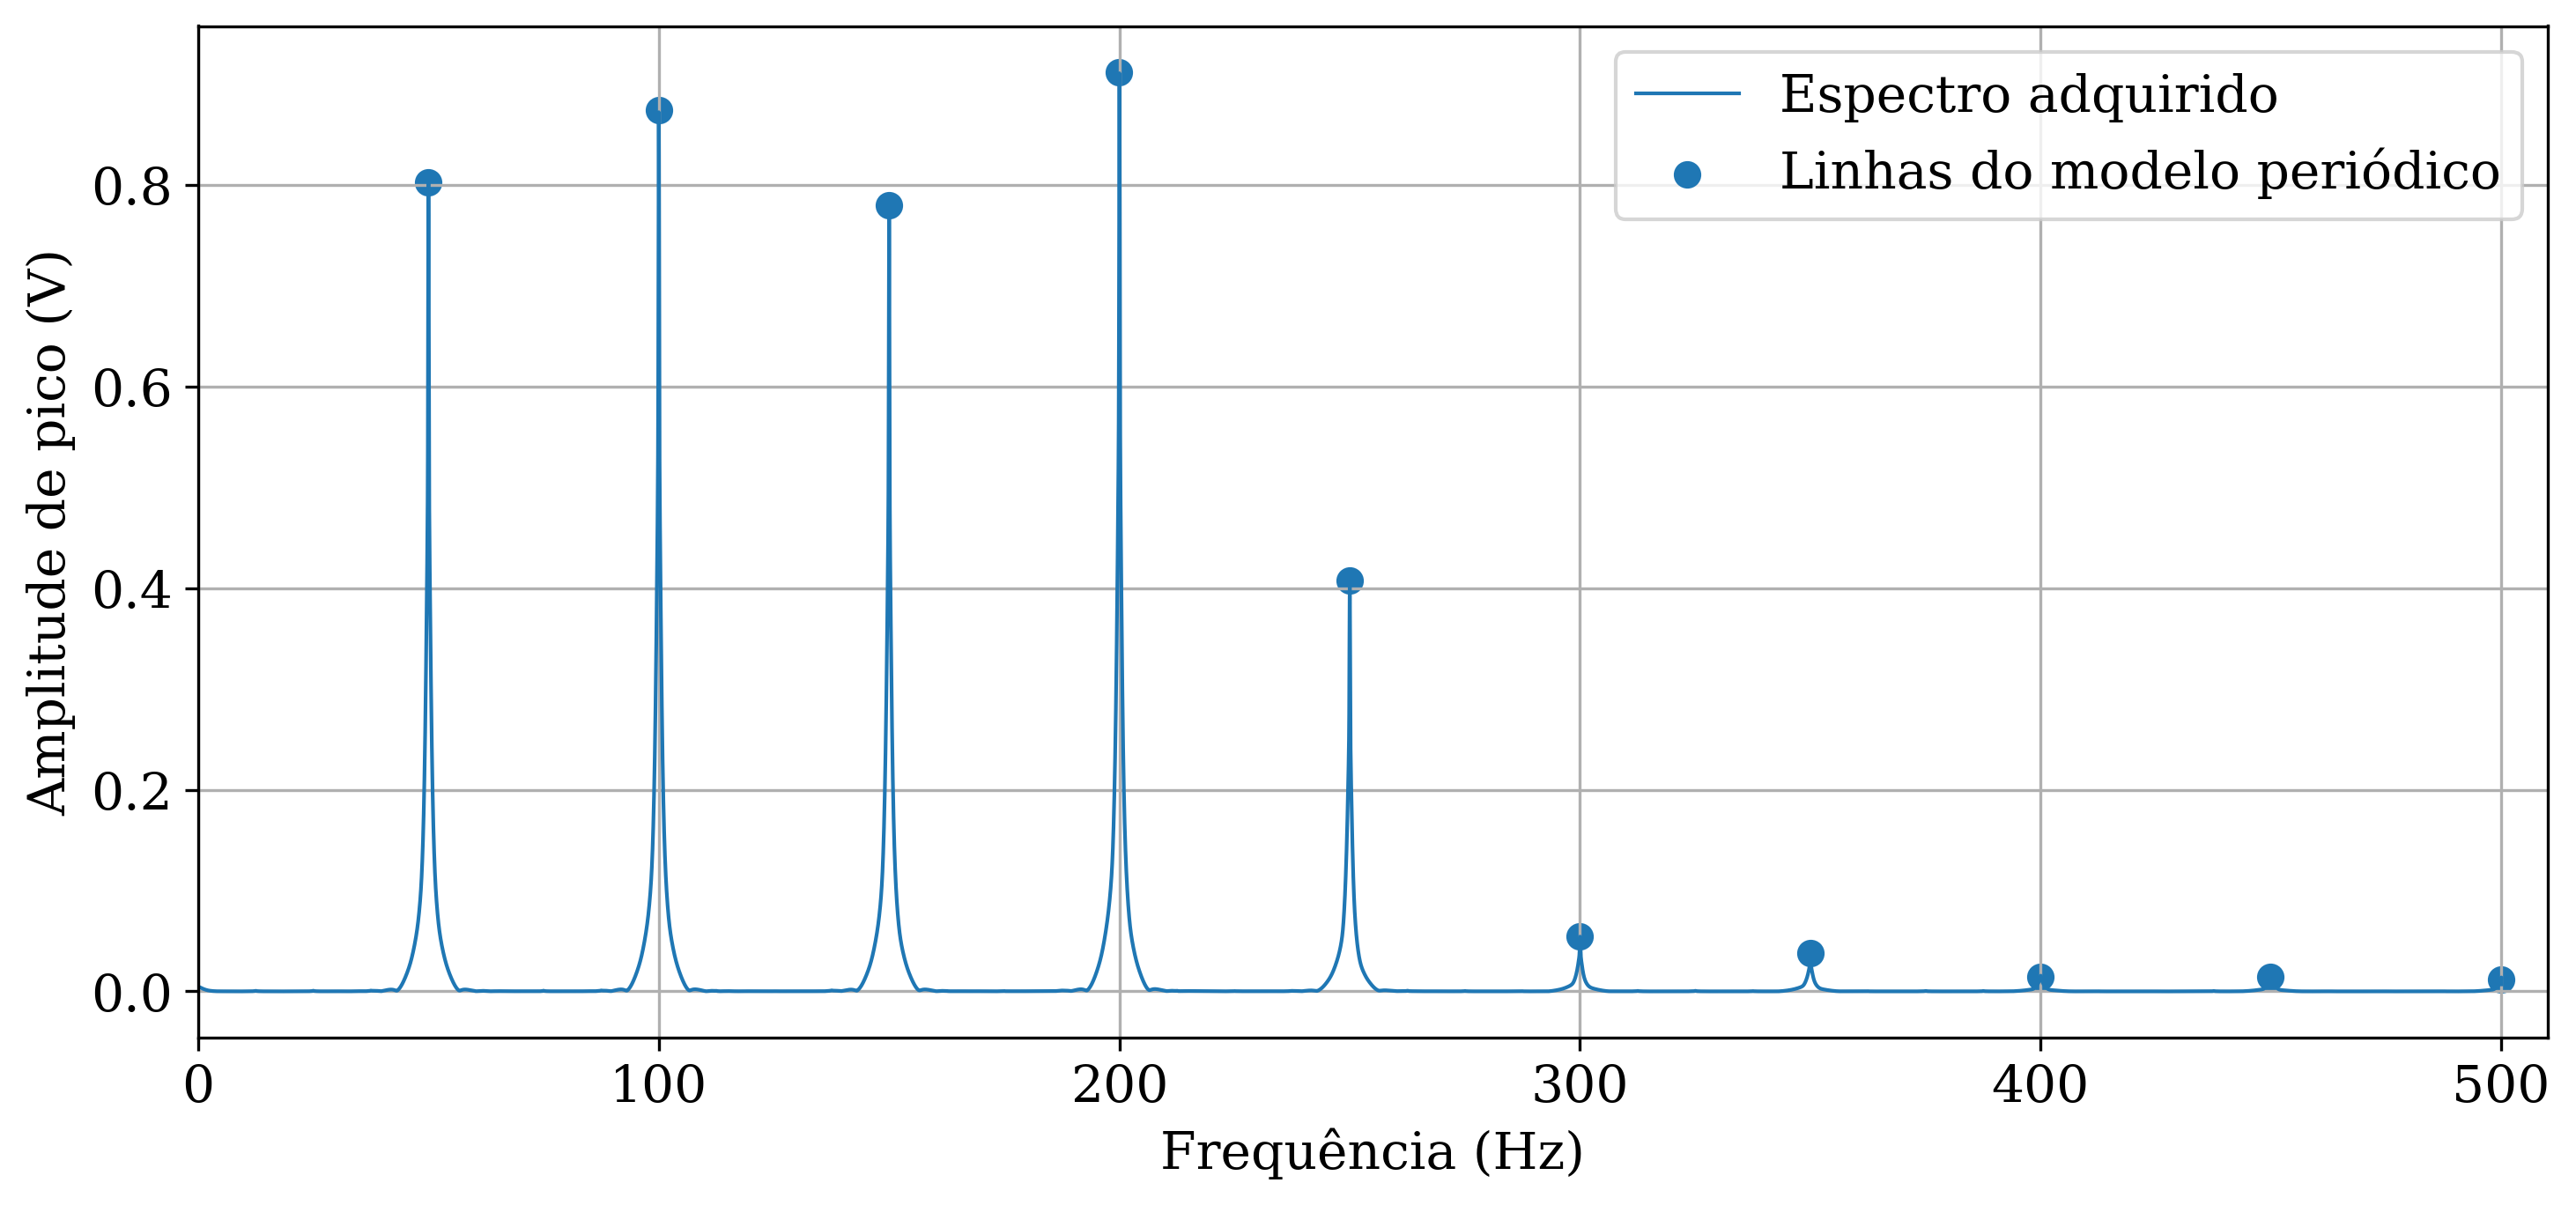
\includegraphics[width=\textwidth]{figuras/figura_sinc_espectro.png}
    \caption[Espectro do sinal sinc periódico]
    {Espectro de amplitude do sinal sinc periódico no intervalo de 0 a 500~Hz. A linha contínua representa o espectro adquirido, enquanto os marcadores indicam as linhas espectrais do modelo periódico, posicionadas em múltiplos de aproximadamente 50~Hz, correspondente à frequência de repetição do sinal. Observa-se maior amplitude nas componentes entre 50 e 200~Hz, seguida de acentuada redução a partir de 250~Hz.}
    \label{fig:sinc_espectro}
\end{figure}

A maior linha espectral foi identificada em 199,9926~Hz, com amplitude de pico de 0,9118~V. Em relação a essa componente, as linhas de 50, 100 e 150~Hz apresentaram níveis de $-1,1138$, $-0,3700$ e $-1,3643$~dBc, respectivamente.

A componente de aproximadamente 250~Hz apresentou nível de $-6,9899$~dBc, indicando o início da redução mais acentuada do envelope espectral. A última linha localizada acima do nível de $-3$~dB ocorreu em aproximadamente 200~Hz. A interpolação entre as linhas de 200 e 250~Hz resultou em uma frequência de corte aproximada de 221,45~Hz.

A borda nominal considerada para o lóbulo espectral principal foi de aproximadamente 249,99~Hz. A primeira linha fortemente atenuada foi encontrada em aproximadamente 299,99~Hz, com nível de $-24,48$~dBc. As componentes de 350, 400, 450 e 500~Hz permaneceram entre aproximadamente $-27,65$ e $-38,05$~dBc.

A largura unilateral aproximada do lóbulo principal foi de 249,99~Hz, correspondendo a uma largura bilateral próxima de 499,98~Hz. Esse valor se aproximou do limite de Nyquist de aproximadamente 500,08~Hz utilizado na análise.

A Figura~\ref{fig:sinc_componentes_relativas} apresenta as amplitudes relativas das linhas espectrais e evidencia a transição entre a região principal, a componente de 250~Hz e a região fortemente atenuada iniciada em 300~Hz.

\begin{figure}[!htbp]
    \centering
    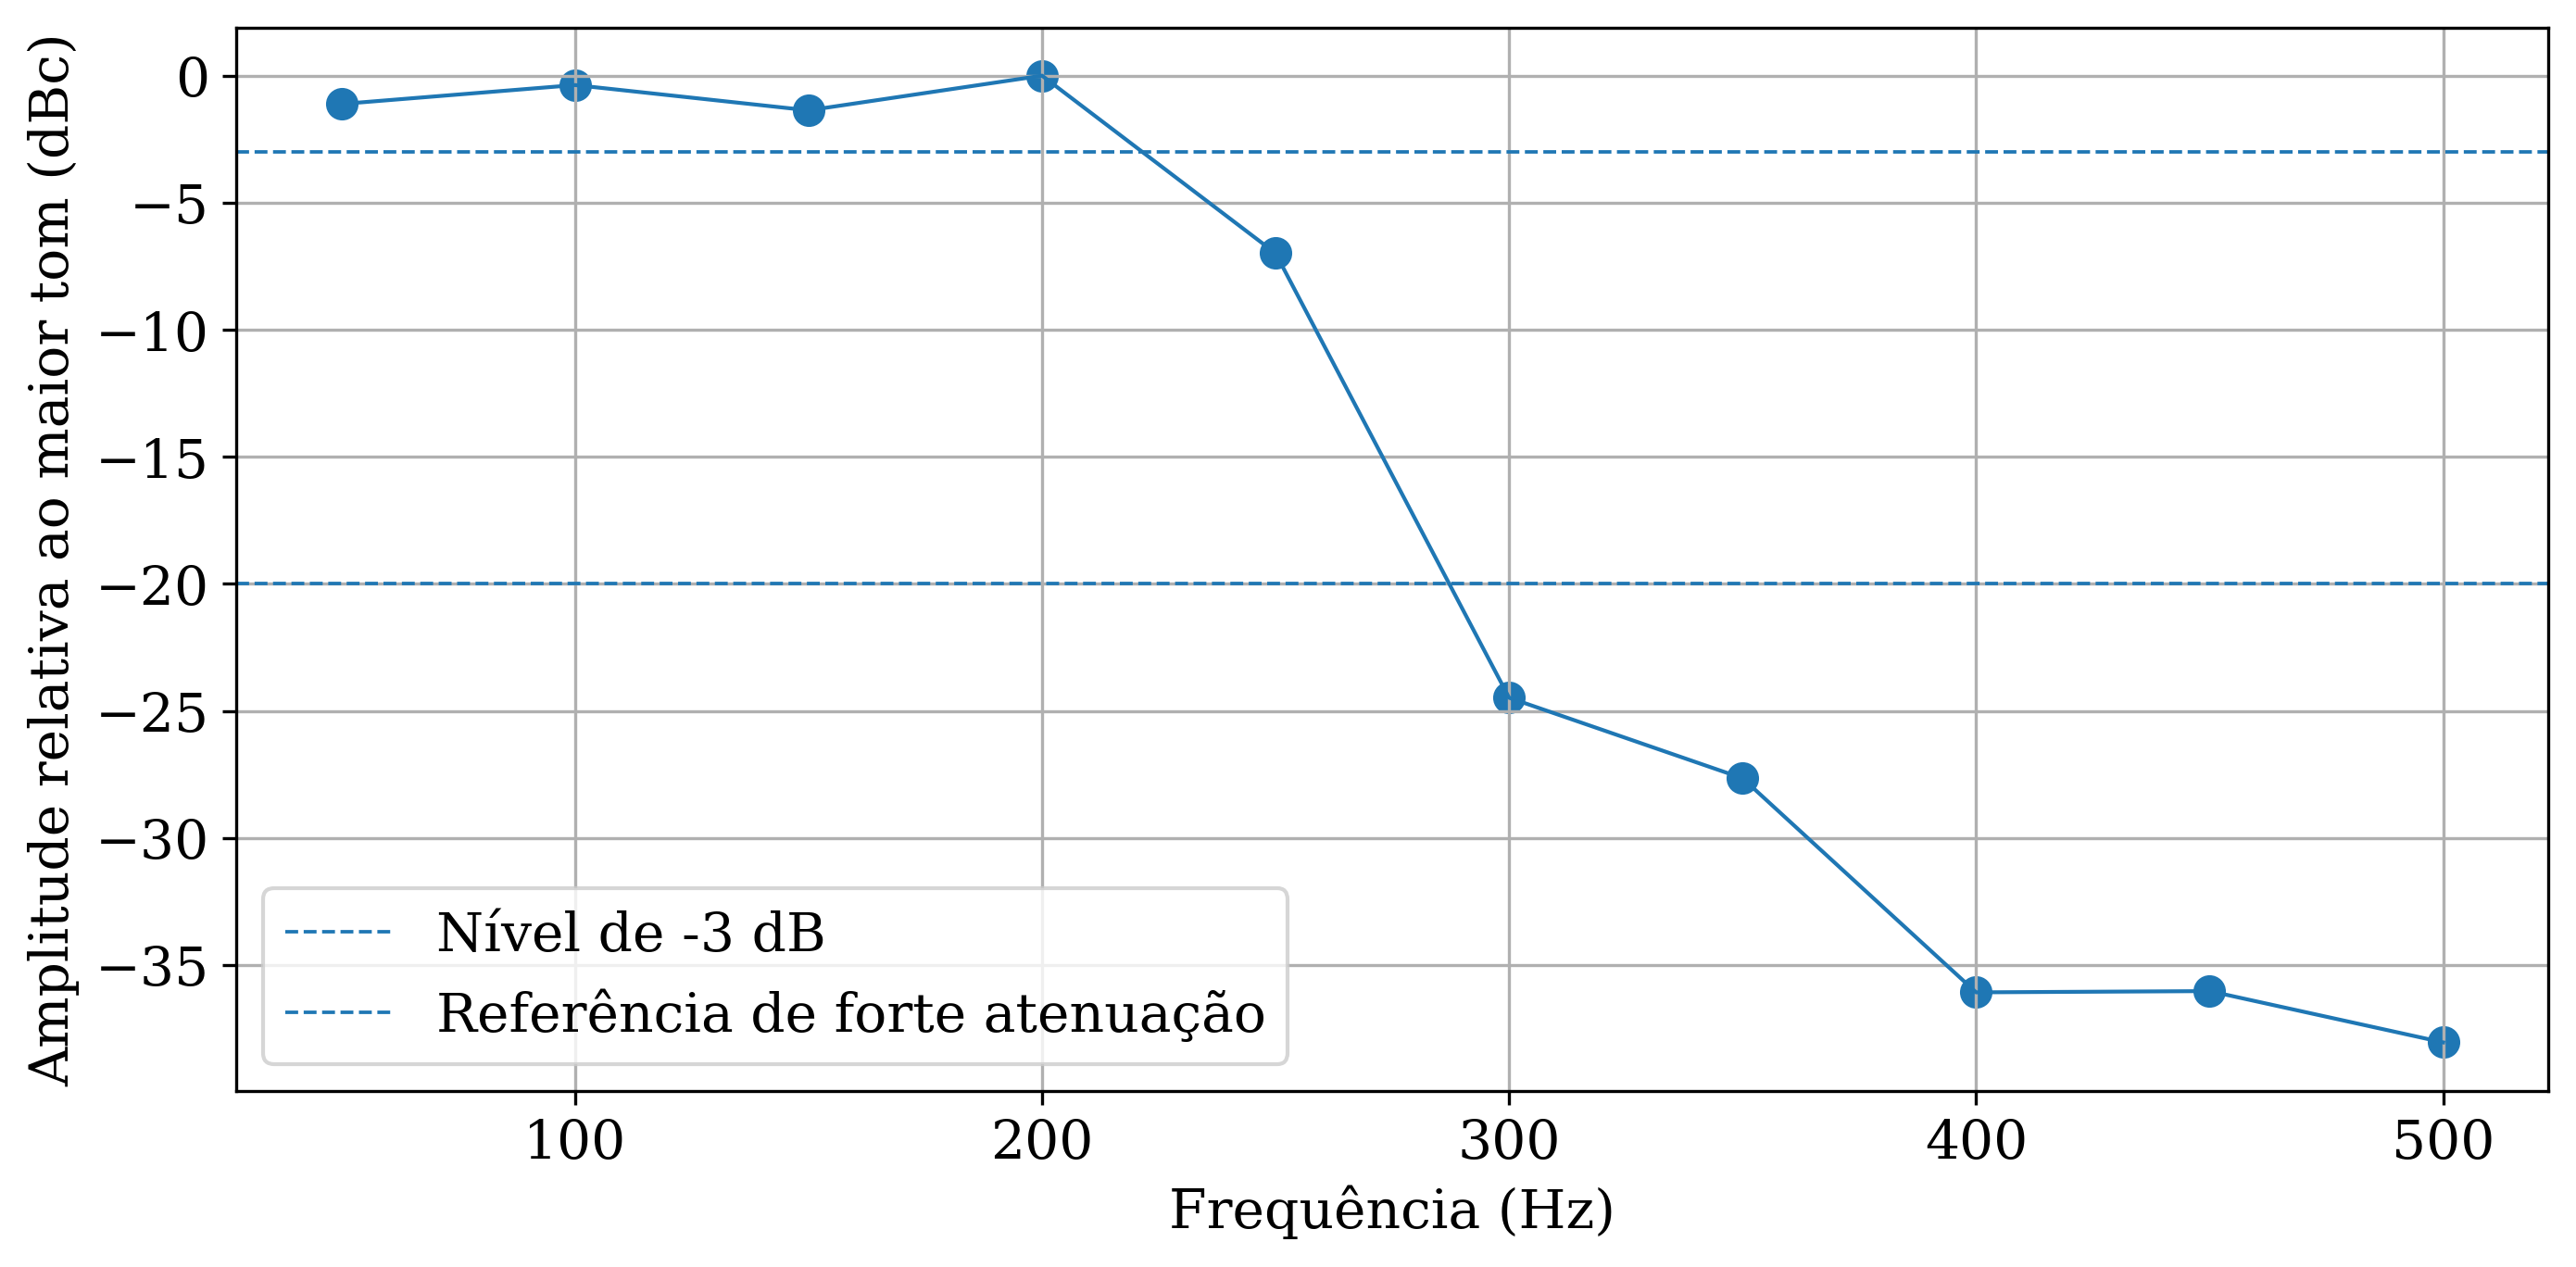
\includegraphics[width=\textwidth]{figuras/figura_sinc_componentes_relativas.png}
    \caption{Amplitudes relativas das linhas espectrais do sinal sinc, utilizando a componente de aproximadamente 200~Hz como referência.}
    \label{fig:sinc_componentes_relativas}
\end{figure}

A Tabela~\ref{tab:componentes_sinc} sintetiza as linhas espectrais identificadas.

\begin{table}[!htbp]
    \centering
    \caption{Componentes espectrais do sinal sinc periódico.}
    \label{tab:componentes_sinc}
    \small
    \begin{tabularx}{\textwidth}{c X X p{2.2cm} p{3.9cm}}
        \hline
        \textbf{Ordem} &
        \textbf{Frequência \mbox{esperada} (Hz)} &
        \textbf{Frequência \mbox{ajustada} (Hz)} &
        \textbf{Amplitude de pico (V)} &
        \textbf{Nível relativo (dBc)} \\
        \hline
        1  & 50  & 49,9982  & 0,8021 & $-1,1138$ \\
        2  & 100 & 99,9963  & 0,8738 & $-0,3700$ \\
        3  & 150 & 149,9945 & 0,7793 & $-1,3643$ \\
        4  & 200 & 199,9926 & 0,9118 & 0,0000 \\
        5  & 250 & 249,9908 & 0,4078 & $-6,9899$ \\
        6  & 300 & 299,9889 & 0,0544 & $-24,4811$ \\
        7  & 350 & 349,9871 & 0,0378 & $-27,6505$ \\
        8  & 400 & 399,9852 & 0,0143 & $-36,0760$ \\
        9  & 450 & 449,9834 & 0,0144 & $-36,0269$ \\
        10 & 500 & 499,9815 & 0,0114 & $-38,0452$ \\
        \hline
    \end{tabularx}
\end{table}

Após a remoção do modelo periódico, a maior componente residual foi encontrada em aproximadamente 387,56~Hz, com nível de $-63,49$~dBc em relação à maior linha do sinal. As demais componentes residuais permaneceram abaixo de aproximadamente $-64,3$~dBc, indicando elevada correspondência entre o registro e o modelo periódico utilizado.

\subsubsection{Discussão dos resultados}
\label{subsubsec:discussao_sinc}

O sinal adquirido preservou o pulso principal, os cruzamentos por zero e a sequência de lóbulos laterais observada no osciloscópio. A simetria aproximada das posições dos mínimos e máximos laterais em torno do pulso principal indicou que a estrutura temporal da forma sinc foi mantida pela cadeia de aquisição.

A largura do lóbulo principal foi representada por pouco menos de três intervalos de amostragem. Embora o ajuste periódico tenha permitido estimar os cruzamentos por zero com resolução inferior ao período de amostragem, essa estimativa depende de interpolação e apresenta menor confiabilidade do que uma medição realizada com taxa de aquisição mais elevada.

A relação entre os domínios do tempo e da frequência foi observada pela presença de um pulso temporal relativamente estreito acompanhado de uma distribuição espectral ampla. Como a forma sinc foi repetida a cada 20~ms, o espectro não apareceu como uma função contínua, mas como linhas espaçadas em aproximadamente 50~Hz sob o envelope espectral da forma gerada.

As componentes entre 50 e 200~Hz permaneceram próximas do nível máximo, enquanto a componente de 250~Hz já apresentou redução de aproximadamente 7~dB. A atenuação superior a 24~dB observada em 300~Hz indicou a passagem para a região externa ao lóbulo espectral principal.

A frequência de corte interpolada de aproximadamente 221,45~Hz deve ser interpretada como uma estimativa baseada em linhas separadas por 50~Hz. A resolução contínua da borda espectral é limitada pela frequência de repetição do sinal, ainda que o espaçamento dos pontos calculados pela FFT seja inferior a esse valor.

A proximidade da largura bilateral estimada com a frequência de Nyquist demonstra que parte do conteúdo associado às frequências mais elevadas foi avaliada próxima ao limite disponível. Consequentemente, uma taxa de aquisição superior permitiria caracterizar com maior margem a região de forte atenuação e verificar a presença de componentes além de 500~Hz sem a possibilidade de sobreposição espectral.

A comparação com o osciloscópio apresentou diferenças inferiores a aproximadamente 5\% para as métricas temporais consideradas. Parte dessas diferenças esteve associada aos diferentes critérios automáticos utilizados para determinar largura, valores extremos e nível médio. Apesar dessas limitações, a forma geral, o período de repetição, a amplitude e a organização temporal e espectral do sinal permaneceram compatíveis com a referência.

De forma geral, o ensaio demonstrou que a plataforma foi capaz de adquirir uma forma de onda com estrutura temporal e espectral mais complexa, preservando o pulso principal, os lóbulos laterais, a frequência de repetição e a distribuição das principais linhas espectrais.

% ----------------------------------------------------------------------------
\subsection{Síntese dos ensaios com sinais conhecidos}
\label{subsec:sintese_sinais_conhecidos}

Os ensaios com sinais conhecidos permitiram avaliar a plataforma diante de formas de onda com diferentes frequências, amplitudes e distribuições espectrais. As senoides possibilitaram verificar diretamente a frequência, a amplitude e a distorção introduzida pela cadeia de aquisição. As ondas quadradas foram utilizadas para avaliar a preservação dos patamares, do ciclo de trabalho, das transições e das componentes harmônicas. Os sinais multitom e sinc, por sua vez, permitiram analisar a resposta do sistema diante de formas de onda com conteúdo espectral composto.

A Tabela~\ref{tab:sintese_sinais_conhecidos} reúne as principais métricas quantitativas obtidas. Para permitir uma comparação uniforme entre os ensaios, as frequências e amplitudes de referência correspondem aos valores configurados no gerador. As comparações específicas com as medidas fornecidas pelo osciloscópio foram apresentadas nas subseções de cada sinal.

Para as senoides, o sinal multitom e o sinal sinc, a amplitude apresentada na tabela corresponde à amplitude pico a pico observada no registro. Para as ondas quadradas, foi utilizada a diferença entre os patamares superior e inferior, por representar melhor a amplitude regular da forma de onda sem incorporar diretamente as excursões transitórias de \textit{overshoot} e \textit{undershoot}. No sinal multitom, a frequência indicada corresponde à frequência-base e ao espaçamento nominal entre os tons. Para o sinal sinc, corresponde à frequência de repetição dos pulsos.

\begin{landscape}
\begin{table}[p]
    \centering
    \caption{Síntese das principais métricas obtidas nos ensaios com sinais conhecidos.}
    \label{tab:sintese_sinais_conhecidos}
    \small
    \renewcommand{\arraystretch}{1.25}
    \begin{tabularx}{\linewidth}{p{2.0cm} c c p{1.5cm} c c p{1.5cm} X}
        \hline
        \textbf{Sinal} &
        \textbf{$f_{\mathrm{ref}}$ (Hz)} &
        \textbf{$f_{\mathrm{med}}$ (Hz)} &
        \textbf{Erro de $f$ (\%)} &
        \textbf{$A_{\mathrm{ref}}$ (V)} &
        \textbf{$A_{\mathrm{med}}$ (V)} &
        \textbf{Erro de $A$ (\%)} &
        \textbf{Principal observação} \\
        \hline

        Senoide de 100~Hz &
        100,0000 &
        99,99635 &
        $-0,00365$ &
        2,000 &
        2,0588 &
        $+2,94$ &
        A forma temporal foi representada por aproximadamente dez amostras por período, com elevada correspondência ao ajuste senoidal e SFDR de 42,89~dB. \\

        Senoide de 450~Hz &
        450,0000 &
        449,98355 &
        $-0,00366$ &
        2,000 &
        2,0375 &
        $+1,88$ &
        A frequência fundamental foi preservada, mas o sinal apresentou somente 2,22 amostras por período, dificultando sua representação temporal e permitindo o rebatimento de componentes harmônicas. \\

        Onda quadrada de 5~Hz &
        5,0000 &
        4,99995 &
        $-0,00101$ &
        5,000 &
        5,1022 &
        $+2,04$ &
        Os patamares, o período e o ciclo de trabalho foram preservados. As primeiras harmônicas ímpares apresentaram amplitudes praticamente coincidentes com os valores teóricos. \\

        Onda quadrada de 50~Hz &
        50,0000 &
        49,99964 &
        $-0,00072$ &
        5,000 &
        5,0337 &
        $+0,67$ &
        A frequência, a amplitude e o ciclo de trabalho apresentaram elevada correspondência, mas as harmônicas de maior ordem sofreram atenuação crescente com a aproximação do limite de Nyquist. \\

        Multitom &
        50,0000 &
        49,9981 &
        $-0,00371$ &
        5,000 &
        5,0847 &
        $+1,69$ &
        As cinco componentes entre 50 e 250~Hz foram separadas e identificadas. A diferença máxima entre suas amplitudes relativas foi de aproximadamente 0,07~dB. \\

        Sinc periódico &
        50,0000 &
        49,9982 &
        $-0,00369$ &
        5,000 &
        5,0688 &
        $+1,38$ &
        O pulso principal, os cruzamentos por zero e os lóbulos laterais foram preservados. O espectro apresentou linhas discretas sob um envelope amplo, com atenuação acentuada acima de aproximadamente 250~Hz. \\

        \hline
    \end{tabularx}
\end{table}
\end{landscape}

Os erros relativos de frequência permaneceram inferiores a 0,004\% em todos os ensaios. O menor erro foi observado para a onda quadrada de 50~Hz, com diferença de aproximadamente $-0,00072$\%, enquanto os maiores valores ocorreram no sinal multitom e no sinal sinc, ainda assim inferiores a 0,004\%. Essa proximidade foi observada desde os sinais de baixa frequência até a senoide de 450~Hz, demonstrando que a plataforma manteve a identificação das componentes fundamentais em toda a faixa avaliada.

As amplitudes medidas também permaneceram próximas dos valores configurados no gerador. Considerando os critérios adotados para cada forma de onda, os erros variaram entre aproximadamente 0,67\% e 2,94\%. A menor diferença foi observada na onda quadrada de 50~Hz, enquanto a maior ocorreu na senoide de 100~Hz. Todos os sinais apresentaram amplitudes medidas ligeiramente superiores aos valores de referência adotados na tabela.

A senoide de 100~Hz apresentou uma das melhores correspondências gerais entre forma temporal, frequência e modelo ajustado. A presença de aproximadamente dez amostras por período permitiu reconhecer diretamente a forma senoidal, enquanto o erro normalizado do ajuste permaneceu inferior a 1\%. A senoide de 450~Hz também apresentou frequência e amplitude próximas aos valores configurados, mas a disponibilidade de apenas 2,22 amostras por período restringiu a representação direta da forma de onda.

As ondas quadradas evidenciaram o efeito da frequência sobre a representação espectral. Na onda de 5~Hz, as primeiras harmônicas ímpares permaneceram praticamente coincidentes com a distribuição teórica de uma onda quadrada ideal. Na onda de 50~Hz, os patamares e o ciclo de trabalho foram preservados, mas as harmônicas de quinta, sétima e nona ordens apresentaram atenuação progressiva. Esse comportamento decorreu da aproximação dessas componentes ao limite de Nyquist e da resposta em frequência da cadeia de aquisição.

O sinal multitom apresentou a melhor evidência de separação de componentes simultâneas. Os cinco tons esperados foram identificados individualmente, com pequena variação de amplitude ao longo da faixa entre 50 e 250~Hz. O sinal sinc demonstrou a capacidade de adquirir uma forma com pulso principal estreito, lóbulos laterais e conteúdo espectral distribuído por uma faixa ampla. Em ambos os casos, as características temporais e espectrais principais permaneceram compatíveis com os sinais observados no osciloscópio.

De forma geral, os ensaios demonstraram que a plataforma foi capaz de identificar corretamente as frequências fundamentais, preservar amplitudes próximas das configurações do gerador e representar formas de onda com diferentes níveis de complexidade. As principais limitações foram observadas nos sinais de maior amplitude, nas formas de onda com transições rápidas e nas componentes localizadas próximas ao limite de Nyquist. Esses resultados indicam que a configuração de 1~kS/s por canal foi adequada para a identificação das componentes principais avaliadas, mas deve ser acompanhada de margens adicionais de amostragem e de controle da faixa de entrada quando forem necessárias maior fidelidade morfológica, caracterização de transições ou análise de harmônicas de ordem elevada.

% ============================================================================
\section{Avaliação do desempenho temporal da aquisição}
\label{sec:desempenho_temporal}

O desempenho temporal da plataforma foi avaliado a partir dos registros produzidos nos ensaios com as senoides de 100~Hz e 450~Hz, com as ondas quadradas de 5~Hz e 50~Hz e com os sinais multitom e sinc. A análise considerou a regularidade dos intervalos entre quadros, a taxa efetiva durante os períodos regulares, a continuidade dos registros e o comportamento da identificação dos canais durante a aquisição multicanal.

Em todas as sessões, a taxa nominal foi configurada em 1~kS/s por canal. Como cada quadro continha os valores associados aos canais adquiridos em um mesmo ciclo de varredura, as marcações temporais permitiram avaliar tanto o espaçamento regular entre quadros consecutivos quanto a ocorrência de intervalos superiores ao período esperado. Os valores apresentados nesta seção foram obtidos diretamente dos registros armazenados, sem interpolação das regiões identificadas como descontínuas.

\subsection{Taxa efetiva de aquisição}
\label{subsec:taxa_efetiva}

A taxa efetiva calculada exclusivamente a partir dos intervalos considerados regulares permaneceu próxima da taxa nominal de 1~kS/s nas três sessões analisadas. No ensaio com as senoides de 100~Hz e 450~Hz, o período médio entre quadros regulares foi de 999,862~$\mu$s, correspondente a uma taxa média de 1000,138~Hz. No ensaio com as ondas quadradas, o período médio foi de 999,852~$\mu$s, resultando em 1000,148~Hz. Para os sinais multitom e sinc, foi obtido período médio de 999,838~$\mu$s e taxa efetiva de 1000,162~Hz.

Os erros relativos da taxa média nos intervalos regulares foram de $+0,0138$\%, $+0,0148$\% e $+0,0162$\%, respectivamente. Dessa forma, a maior diferença em relação ao valor nominal permaneceu inferior a 0,017\%, indicando que, durante os trechos sem lacunas temporais, o ciclo de aquisição manteve frequência próxima à configuração prevista.

A dispersão dos intervalos regulares também apresentou comportamento semelhante entre as sessões. Os percentis de 95\% permaneceram entre 1003 e 1004~$\mu$s, enquanto os percentis de 99\% ficaram entre 1005 e 1006~$\mu$s. Os menores intervalos observados variaram entre 934 e 935~$\mu$s. Esses resultados mostram que a maior parte dos intervalos permaneceu concentrada nas proximidades de 1~ms.

Os maiores intervalos registrados foram de 107,733~ms no ensaio com as senoides, 99,057~ms no ensaio com as ondas quadradas e 223,310~ms no ensaio com os sinais complexos. Esses valores não representam a dispersão típica dos intervalos regulares, mas correspondem às lacunas temporais discutidas na Subseção~\ref{subsec:continuidade_registros}.

A Tabela~\ref{tab:taxa_efetiva_sessoes} apresenta as principais métricas associadas à taxa de aquisição.

\begin{table}[!htbp]
    \centering
    \caption{Taxa efetiva e distribuição dos intervalos entre quadros nas sessões analisadas.}
    \label{tab:taxa_efetiva_sessoes}
    \small
        \begin{tabularx}{\textwidth}{p{4.5cm} X X X}
            \hline
            \textbf{Ensaio} &
            \textbf{Senoides de 100 e 450~Hz} &
            \textbf{Ondas quadradas de 5 e 50~Hz} &
            \textbf{Multitom e sinc} \\
            \hline
            \textbf{Taxa nominal (Hz)}
            & 1000,000 & 1000,000 & 1000,000 \\

            \textbf{Período médio ($\mu$s)}
            & 999,862 & 999,852 & 999,838 \\

            \textbf{Taxa regular (Hz)}
            & 1000,138 & 1000,148 & 1000,162 \\

            \textbf{Erro da taxa (\%)}
            & $+0,0138$ & $+0,0148$ & $+0,0162$ \\

            \textbf{$\Delta t_{\min}$ ($\mu$s)}
            & 934 & 935 & 934 \\

            \textbf{$P_{95}$ ($\mu$s)}
            & 1003 & 1003 & 1004 \\

            \textbf{$P_{99}$ ($\mu$s)}
            & 1005 & 1005 & 1006 \\

            \textbf{$\Delta t_{\max}$ (ms)}
            & 107,733 & 99,057 & 223,310 \\
            \hline
        \end{tabularx}
\end{table}

Quando a taxa foi calculada pela razão entre a quantidade total de quadros recebidos e a duração completa de cada registro, incluindo as lacunas, foram obtidos valores inferiores: 969,66~Hz para as senoides, 926,40~Hz para as ondas quadradas e 964,95~Hz para os sinais complexos. A diferença entre a taxa regular e a taxa global demonstra que o espaçamento entre quadros permaneceu próximo de 1~ms durante a operação normal, enquanto as interrupções ocasionais reduziram a quantidade efetiva de dados recebidos ao longo de toda a sessão.

\subsection{Continuidade dos registros}
\label{subsec:continuidade_registros}

O registro das senoides de 100~Hz e 450~Hz apresentou duração temporal de 32,603~s, durante a qual foram recebidos 31.615 quadros. A estimativa baseada na grade temporal indicou 32.610 quadros esperados e 995 quadros ausentes, correspondentes a 3,051\% do total estimado. Foram identificados 13 intervalos com perdas, que dividiram o registro em 14 segmentos contíguos. O maior intervalo observado foi de 107,733~ms, associado a uma estimativa de 107 quadros ausentes, enquanto o maior trecho contínuo apresentou duração de 6,812~s.

No ensaio com as ondas quadradas de 5~Hz e 50~Hz, a duração temporal foi de 31,092~s. Foram recebidos 28.805 quadros diante de uma estimativa de 31.098 quadros esperados, resultando em 2.293 quadros ausentes e percentual de perda estimado em 7,373\%. Foram encontrados 31 intervalos com perdas e 32 segmentos contíguos. A maior lacuna foi de 99,057~ms, correspondente a aproximadamente 98 quadros ausentes, e o maior segmento contínuo apresentou duração de 1,570~s.

A sessão com os sinais multitom e sinc apresentou duração temporal de 42,277~s e 40.796 quadros recebidos. A quantidade estimada de quadros esperados foi de 42.284, resultando em 1.488 quadros ausentes e percentual de perda de 3,519\%. Foram identificados 16 intervalos com perdas e 17 segmentos contíguos. O maior intervalo observado foi de 223,310~ms, associado a aproximadamente 222 quadros ausentes. Apesar dessa lacuna, a sessão apresentou o maior trecho contínuo entre os ensaios, com duração de 10,220~s.

A Tabela~\ref{tab:continuidade_sessoes} sintetiza as métricas de continuidade dos registros.

\begin{table}[!htbp]
    \centering
    \caption{Continuidade temporal das sessões utilizadas na avaliação da aquisição.}
    \label{tab:continuidade_sessoes}
    \small
    \begin{tabularx}{\textwidth}{
        >{\raggedright\arraybackslash}p{5.2cm}
        *{3}{>{\centering\arraybackslash}X}
    }
        \hline
        \textbf{Ensaio} &
        \textbf{Senoides de 100~Hz e 450~Hz} &
        \textbf{Ondas quadradas de 5~Hz e 50~Hz} &
        \textbf{Multitom e sinc} \\
        \hline

        \textbf{Duração (s)}
        & 32,603 & 31,092 & 42,277 \\

        \textbf{Quadros recebidos}
        & 31.615 & 28.805 & 40.796 \\

        \textbf{Quadros esperados}
        & 32.610 & 31.098 & 42.284 \\

        \textbf{Perdas estimadas}
        & 995 & 2.293 & 1.488 \\

        \textbf{Perda (\%)}
        & 3,051 & 7,373 & 3,519 \\

        \textbf{Lacunas}
        & 13 & 31 & 16 \\

        \textbf{Maior lacuna (ms)}
        & 107,733 & 99,057 & 223,310 \\

        \textbf{Maior trecho contínuo (s)}
        & 6,812 & 1,570 & 10,220 \\

        \hline
    \end{tabularx}
\end{table}

Considerando conjuntamente as três sessões, foram recebidos 101.216 quadros diante de uma estimativa de 105.992 quadros esperados. A diferença acumulada foi de 4.776 quadros, correspondente a aproximadamente 4,506\%. Foram identificadas 60 lacunas temporais ao longo dos registros analisados. Esse valor agregado deve ser interpretado apenas como síntese do conjunto experimental, pois as sessões apresentaram durações e distribuições de lacunas distintas.

Não foram observados saltos nos campos \texttt{sample\_index} ou \texttt{sequence\_id}, nem marcações temporais não monotônicas. Dessa forma, os quadros efetivamente armazenados mantiveram ordenação crescente e coerência interna. As descontinuidades se manifestaram predominantemente pelo aumento do intervalo temporal entre quadros consecutivos, sem inversão da ordem ou repetição dos identificadores registrados.

Embora as lacunas tenham reduzido a continuidade global, todas as sessões apresentaram segmentos contíguos suficientes para a extração das métricas temporais e espectrais utilizadas nos ensaios com sinais conhecidos. As análises de frequência foram realizadas separadamente sobre os segmentos identificados, evitando a união direta de trechos separados por intervalos ausentes.

\subsection{Comportamento da aquisição multicanal}
\label{subsec:desempenho_multicanal}

Os ensaios foram realizados com dois sinais de referência aplicados simultaneamente a pares diferenciais distintos do ADS1256. Cada quadro transmitido manteve posições fixas para os valores dos canais, de modo que a associação física definida na configuração da sessão foi preservada nos arquivos armazenados. A inspeção temporal e espectral não indicou troca de canais ao longo dos registros.

Nas sessões analisadas, os valores dos diferentes canais compartilharam o mesmo número sequencial e a mesma marcação temporal de quadro. Essa organização permitiu comparar diretamente os sinais adquiridos no mesmo ciclo de varredura e preservou o alinhamento entre os canais nos arquivos exportados.

No ensaio com as senoides, a componente de aproximadamente 450,01~Hz observada no canal de 100~Hz apresentou nível de $-52,33$~dBc em relação à sua componente fundamental. No canal de 450~Hz, foi encontrada uma componente próxima de 100,10~Hz com nível de $-42,13$~dBc. Entretanto, essa segunda componente também é compatível com o rebatimento do segundo harmônico de 450~Hz, originalmente localizado próximo de 900~Hz. Assim, sua presença não pode ser atribuída exclusivamente ao acoplamento entre canais.

No ensaio com as ondas quadradas, o canal de 5~Hz apresentou componentes próximas de 249,96, 350,03 e 450,03~Hz, com níveis entre aproximadamente $-53,53$ e $-55,84$~dBc. Essas frequências coincidem com harmônicas ímpares do sinal de 50~Hz adquirido simultaneamente, o que sugere uma possível contribuição de acoplamento entre os canais. No canal de 50~Hz, as maiores componentes não previstas foram observadas próximas de 40,37 e 59,72~Hz, ambas em torno de $-48,2$~dBc. A proximidade de uma dessas componentes com 60~Hz também permite considerar a interferência da rede elétrica como possível origem.

Na aquisição simultânea do multitom e do sinal sinc, cada canal manteve características temporais e espectrais distintas. O multitom apresentou componentes principais entre 50 e 250~Hz, enquanto o sinal sinc apresentou linhas distribuídas sob um envelope espectral próprio. A preservação dessas estruturas distintas nos respectivos canais demonstrou que a organização multicanal foi mantida durante a aquisição.

\subsection{Síntese do desempenho da aquisição}
\label{subsec:sintese_desempenho_aquisicao}

A Tabela~\ref{tab:sintese_desempenho_aquisicao} reúne os principais indicadores temporais obtidos nas três sessões.

\begin{table}[!htbp]
    \centering
    \caption{Síntese do desempenho temporal da aquisição nos ensaios realizados.}
    \label{tab:sintese_desempenho_aquisicao}
    \small
    \begin{tabularx}{\textwidth}{
        >{\raggedright\arraybackslash}p{5.3cm}
        *{3}{>{\centering\arraybackslash}X}
    }
        \hline
        \textbf{Ensaio} &
        \textbf{Senoides de 100~Hz e 450~Hz} &
        \textbf{Ondas quadradas de 5~Hz e 50~Hz} &
        \textbf{Multitom e sinc} \\
        \hline

        \textbf{Taxa nominal (Hz)}
        & 1000,000 & 1000,000 & 1000,000 \\

        \textbf{Taxa regular (Hz)}
        & 1000,138 & 1000,148 & 1000,162 \\

        \textbf{Erro da taxa (\%)}
        & $+0,0138$ & $+0,0148$ & $+0,0162$ \\

        \textbf{Taxa global (Hz)}
        & 969,66 & 926,40 & 964,95 \\

        \textbf{Perda estimada (\%)}
        & 3,051 & 7,373 & 3,519 \\

        \textbf{Maior lacuna (ms)}
        & 107,733 & 99,057 & 223,310 \\

        \textbf{Maior trecho contínuo (s)}
        & 6,812 & 1,570 & 10,220 \\

        \hline
    \end{tabularx}
\end{table}


Durante os intervalos regulares, a plataforma manteve taxa de aquisição muito próxima de 1~kS/s por canal, com erro inferior a 0,017\% em todas as sessões e percentil de 99\% dos intervalos limitado a aproximadamente 1006~$\mu$s. Esse comportamento foi suficiente para identificar corretamente as frequências fundamentais e obter as métricas temporais e espectrais dos sinais avaliados.

A principal limitação foi observada na continuidade global. As lacunas reduziram a taxa média calculada sobre a duração completa para valores entre aproximadamente 926 e 970~Hz. O ensaio com as ondas quadradas apresentou o maior percentual de perda e o menor trecho contínuo, enquanto a sessão com os sinais complexos apresentou a maior lacuna isolada, mas também o maior segmento contínuo.

Os resultados mostram que a limitação principal não esteve na frequência do ciclo regular de aquisição, mas na ocorrência ocasional de interrupções mais longas. Para ensaios de bancada e processamento posterior, essas interrupções puderam ser tratadas pela seleção de segmentos contíguos. Entretanto, em aplicações que dependam de monitoramento ininterrupto, análise de eventos transitórios ou sincronização contínua entre sinais fisiológicos, a redução dessas lacunas constitui um aspecto importante para o aperfeiçoamento da plataforma.

A continuidade poderá ser aprimorada por modificações na organização da transmissão e do armazenamento, como uso de buffers adicionais no firmware, envio não bloqueante pela interface USB, agrupamento de múltiplos quadros por transferência e redução de operações concorrentes durante a aquisição. Essas possibilidades devem ser avaliadas em ensaios específicos, pois alterações no fluxo de dados também podem modificar a latência, o consumo de memória e a capacidade de visualização em tempo próximo ao real.

% ============================================================================
\section{Resultados da aquisição dos sinais fisiológicos}
\label{sec:resultados_sinais_fisiologicos}

A avaliação com sinais fisiológicos foi realizada para verificar o funcionamento da plataforma em uma condição de aquisição multicanal envolvendo sinais reais e módulos de condicionamento distintos. Foram registrados simultaneamente dois canais de eletrocardiograma, denominados ECG~1 e ECG~2, e um canal de fotopletismografia.

Os valores de tensão apresentados correspondem às tensões estimadas na entrada do ADS1256 após o condicionamento realizado pelos respectivos módulos. Portanto, essas amplitudes não correspondem diretamente aos potenciais presentes nos eletrodos ou no tecido e não devem ser interpretadas como medidas clínicas. A análise teve caráter funcional e qualitativo, sendo direcionada à identificação de formas de onda compatíveis com ECG e PPG, à regularidade dos ciclos, à repetibilidade morfológica e à coerência temporal entre os canais.

\subsection{Aquisição simultânea de dois canais de ECG e um canal de PPG}
\label{subsec:aquisicao_simultanea_fisiologicos}

A sessão fisiológica apresentou duração de 29,7495~s e armazenou 29.750 quadros multicanais. A taxa média calculada a partir dos intervalos entre quadros foi de 999,983~Hz, enquanto a mediana correspondeu a 1000,000~Hz. O período mediano foi de 1000~$\mu$s, com intervalo mínimo de 996~$\mu$s, percentil de 99\% igual a 1006~$\mu$s e intervalo máximo de 1007~$\mu$s.

Os canais foram armazenados em posições fixas e identificados como ECG~1, ECG~2, PPG e temperatura auxiliar. Os três sinais analisados compartilharam a mesma sequência e a mesma marcação temporal de quadro, permitindo sua representação em uma base temporal comum e a comparação dos eventos detectados.

A Figura~\ref{fig:multicanal_fisiologicos} apresenta um trecho representativo de 8~s selecionado entre 11,5 e 19,5~s da sessão. As amplitudes foram normalizadas e deslocadas verticalmente apenas para facilitar a visualização conjunta. Observam-se complexos de maior amplitude nos dois canais de ECG e oscilações pulsáteis regulares no canal de PPG.

\begin{figure}[!htbp]
    \centering
    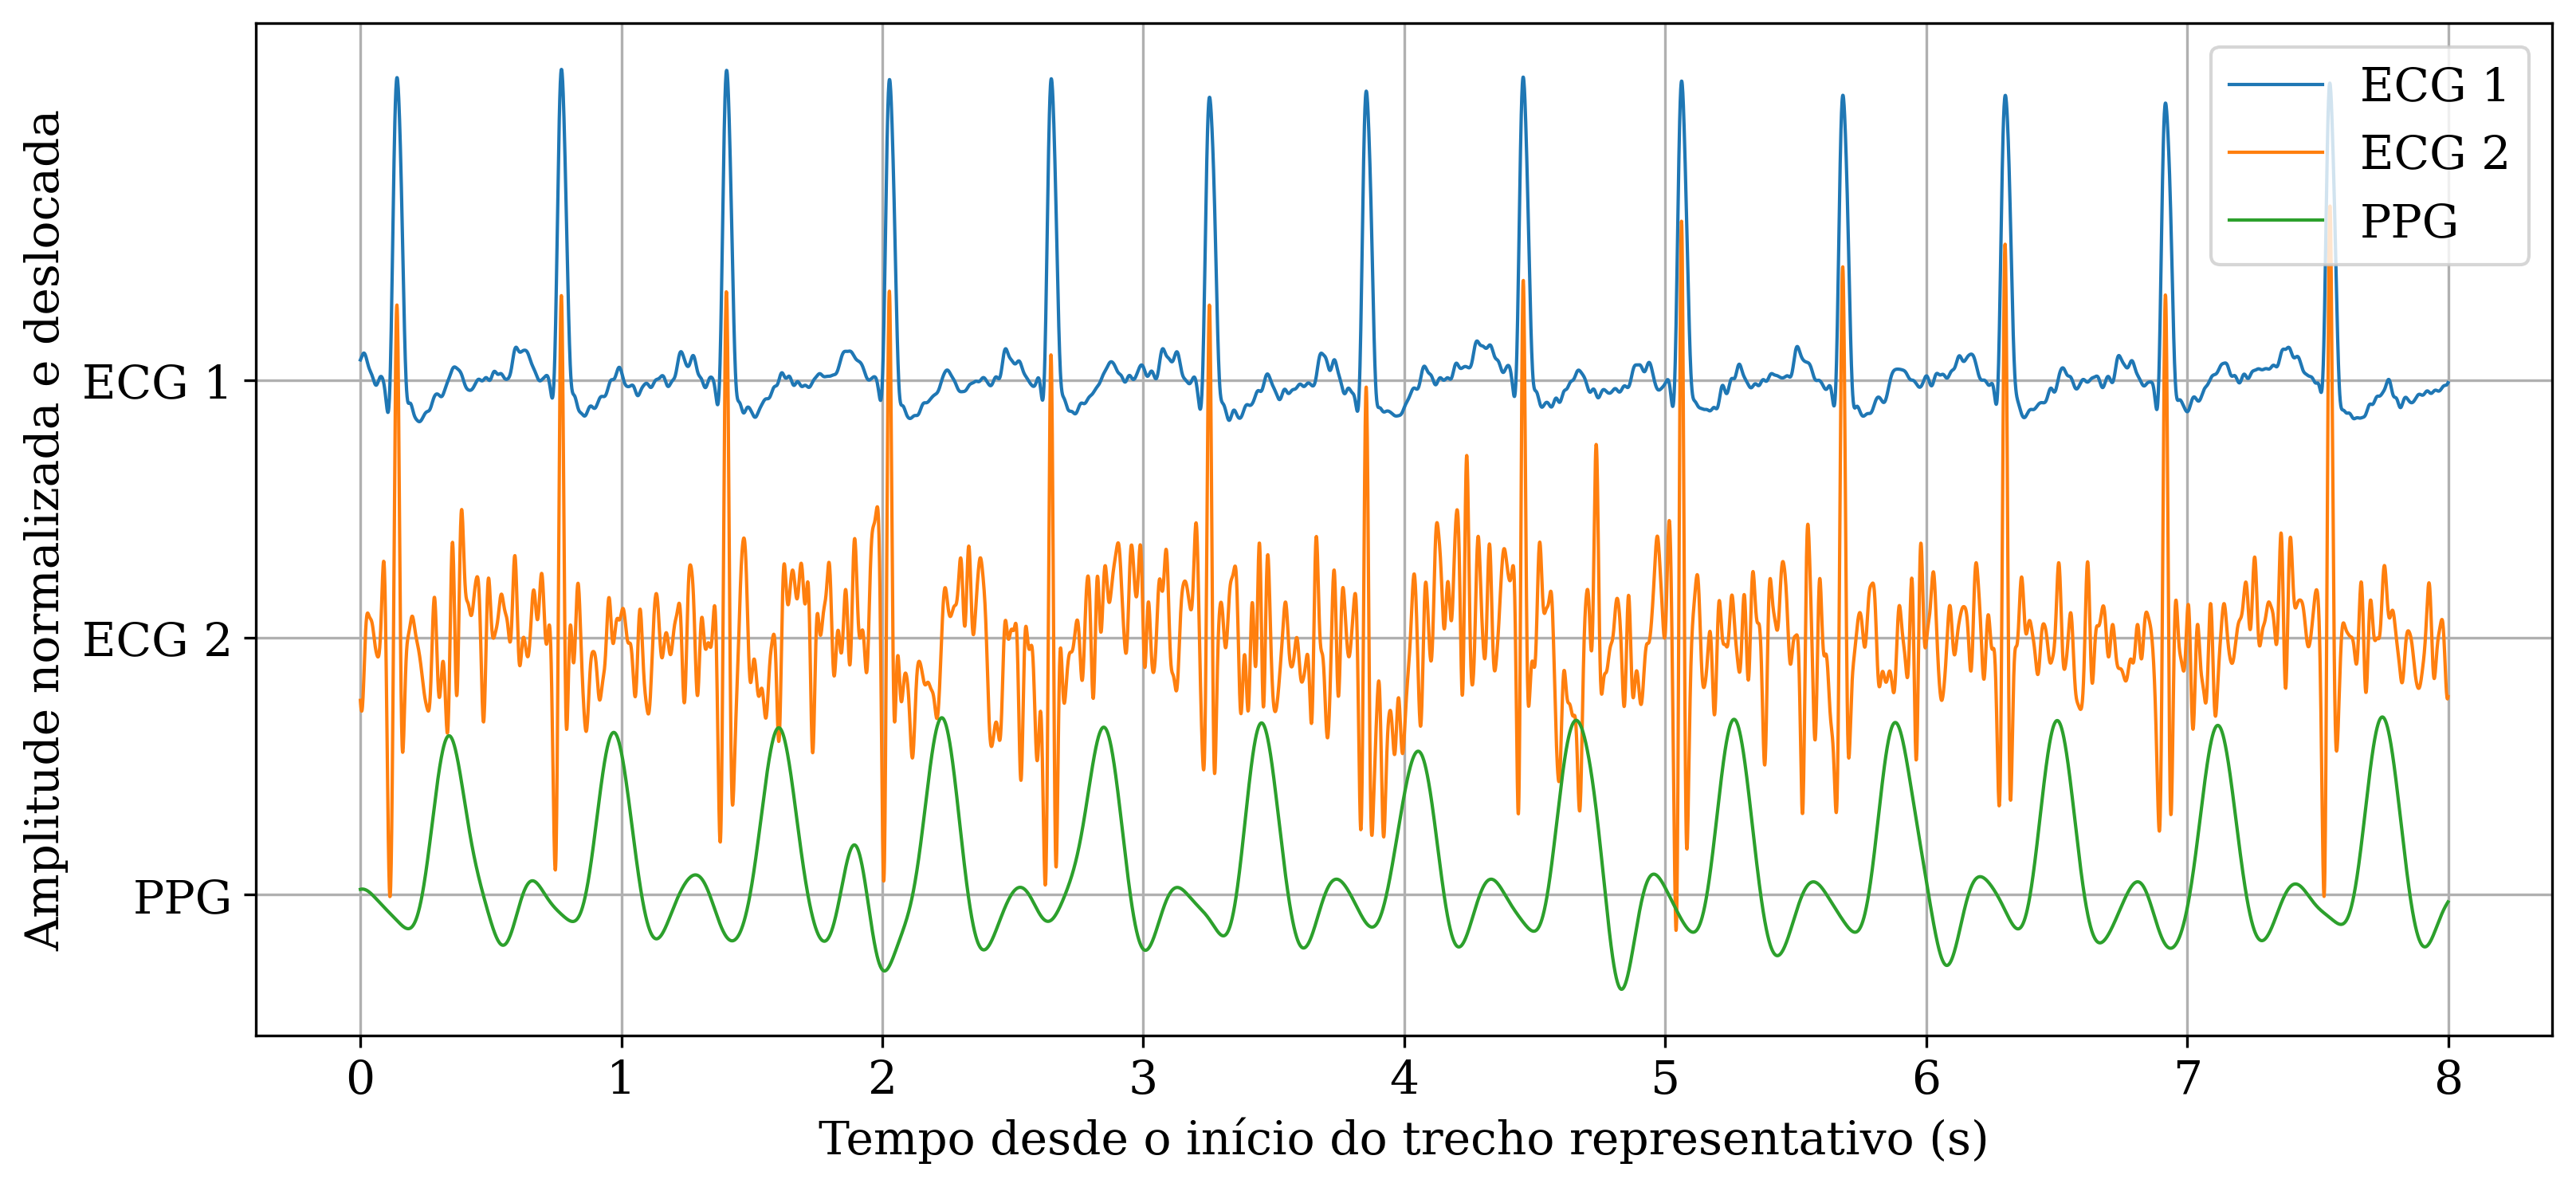
\includegraphics[width=\textwidth]{figuras/figura_multicanal_ecg1_ecg2_ppg.png}
    \caption[Aquisição simultânea dos sinais ECG e PPG]
    {Trecho representativo de 8~s da aquisição simultânea dos canais ECG~1, ECG~2 e PPG, apresentados em uma mesma base temporal. As amplitudes de cada canal foram normalizadas e os sinais foram deslocados verticalmente para evitar sobreposição e facilitar a comparação de sua evolução temporal. Os picos recorrentes observados nos dois canais de ECG correspondem à atividade cardíaca detectada eletricamente, enquanto as oscilações do PPG representam a resposta pulsátil periférica associada aos ciclos cardíacos.}
    \label{fig:multicanal_fisiologicos}
\end{figure}

No trecho selecionado foram identificados 13 eventos em cada um dos três canais. Os coeficientes de variação dos intervalos foram de 1,78\% para o ECG~1, 1,75\% para o ECG~2 e 1,75\% para o PPG, indicando que a região escolhida apresentava ciclos regulares e era representativa do comportamento observado na sessão.

\subsection{Resultado do primeiro canal de ECG}
\label{subsec:resultado_ecg_1}

\subsubsection{Representação no domínio do tempo}
\label{subsubsec:ecg_1_tempo}

O primeiro canal de ECG apresentou complexos de elevada amplitude e polaridade positiva, repetidos regularmente ao longo da sessão. Foram detectados 47 eventos associados aos picos R, com amplitude mediana de aproximadamente 802,35~mV na entrada do ADC após o condicionamento. O intervalo entre os percentis de 5\% e 95\% das amplitudes dos picos foi equivalente a aproximadamente 753,50 e 853,57~mV.

A Figura~\ref{fig:ecg1_bruto_filtrado} apresenta o sinal bruto e o sinal filtrado utilizado na análise. O processamento reduziu parte das variações lentas da linha de base e do conteúdo de maior frequência, preservando os complexos de maior amplitude empregados na detecção dos eventos.

\begin{figure}[!htbp]
    \centering
    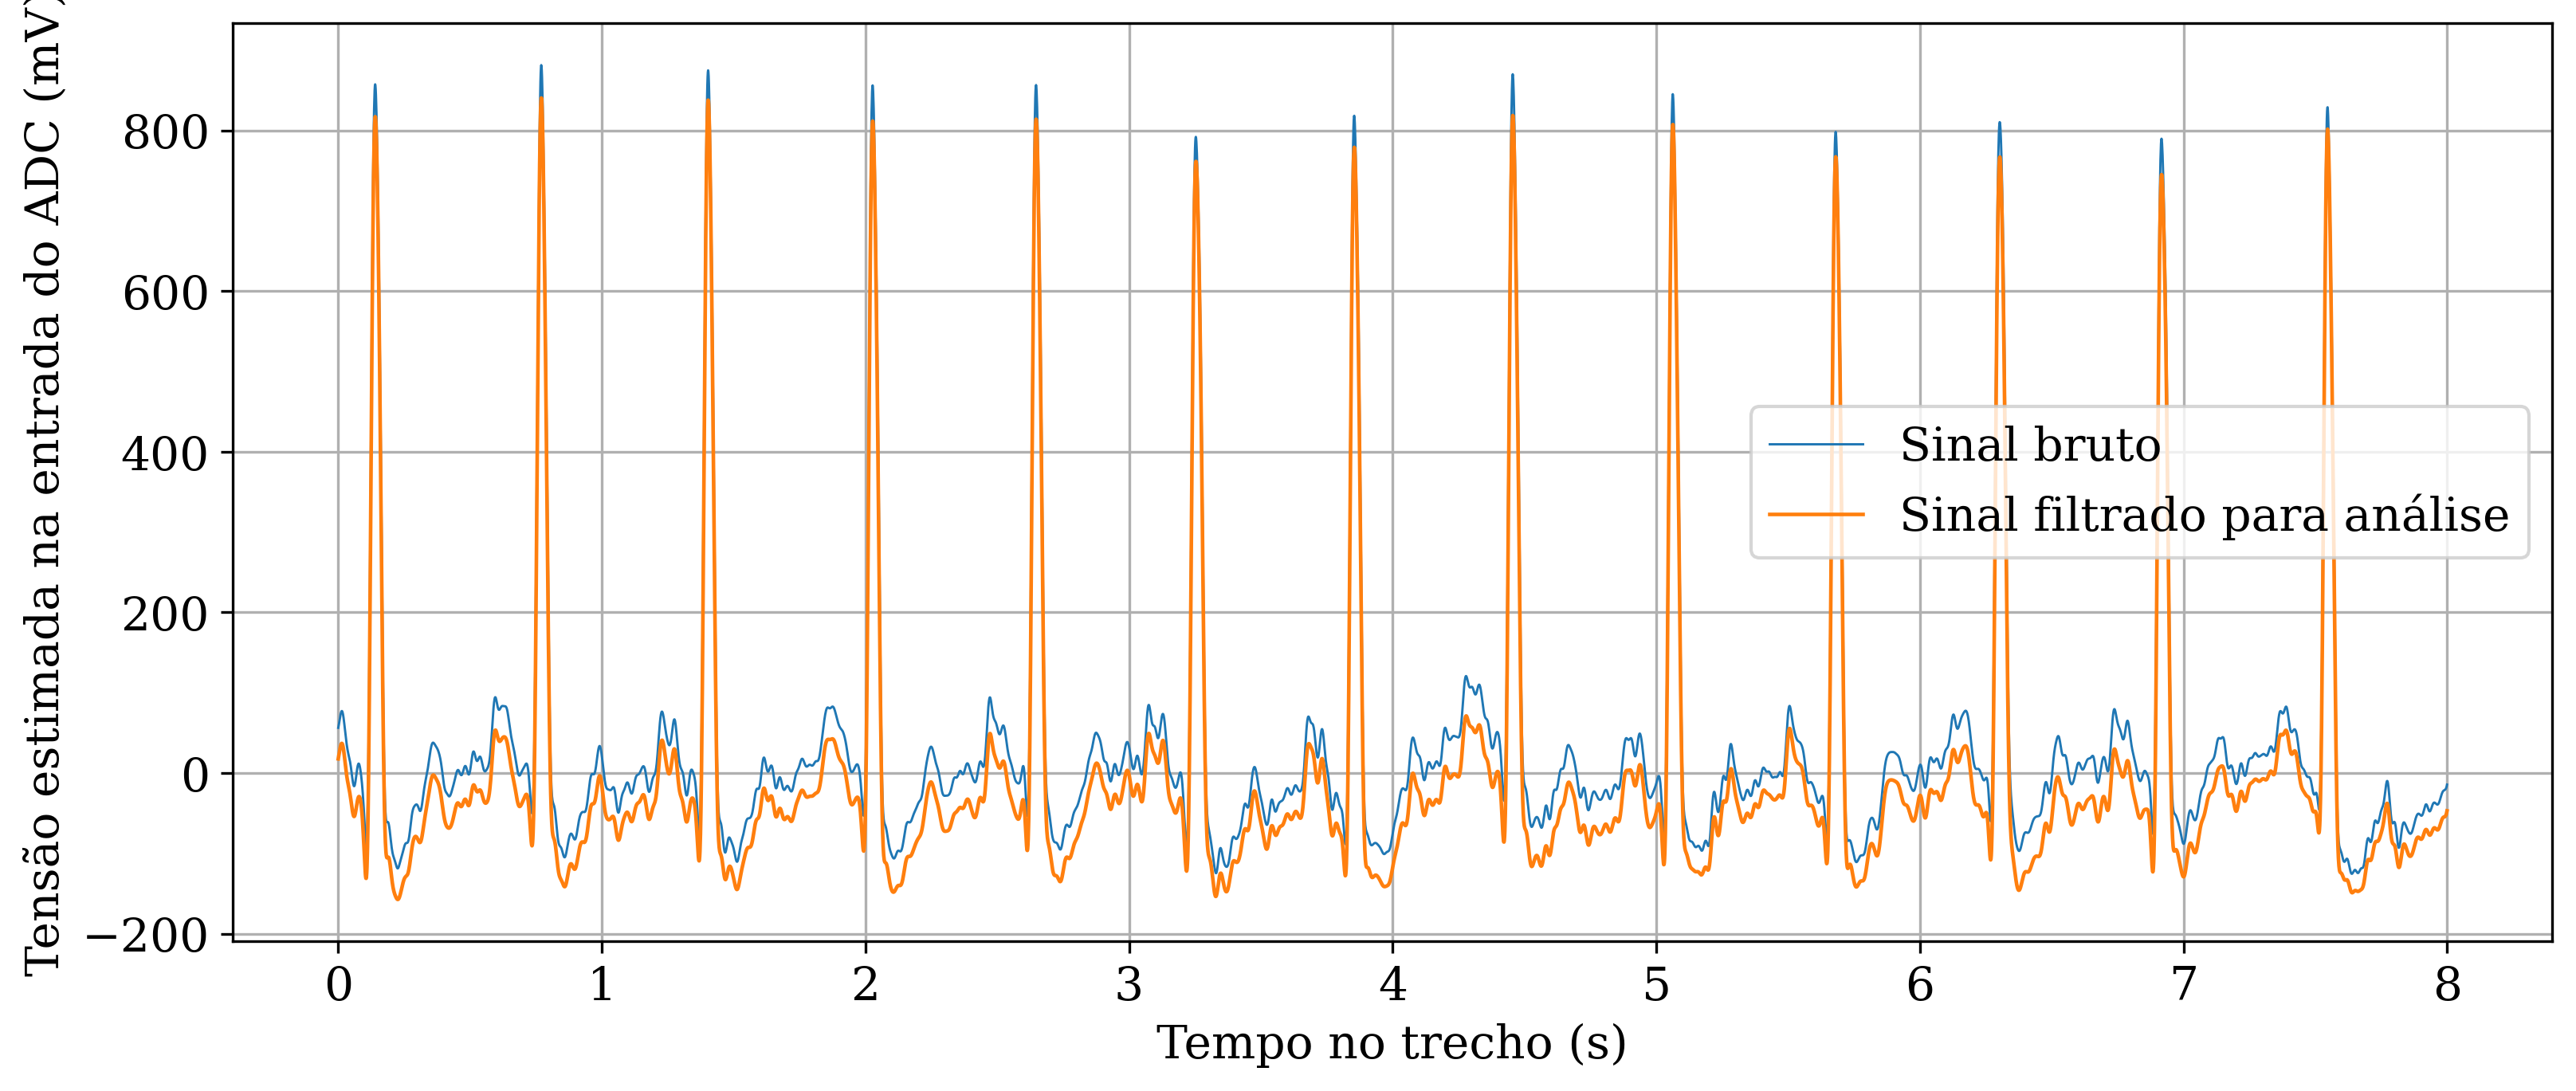
\includegraphics[width=\textwidth]{figuras/figura_ecg1_bruto_filtrado.png}
    \caption[Comparação entre os sinais bruto e filtrado do ECG~1]
    {Comparação, em um trecho representativo de 8~s, entre o sinal bruto do primeiro canal de ECG e o sinal resultante do processamento empregado na análise. A tensão foi estimada na entrada do conversor analógico-digital (ADC) e expressa em milivolts. O sinal filtrado preserva a posição temporal e a amplitude predominante dos complexos QRS, ao mesmo tempo que reduz as flutuações presentes entre os picos, facilitando sua identificação e a análise dos ciclos cardíacos.}
    \label{fig:ecg1_bruto_filtrado}
\end{figure}

A Figura~\ref{fig:ecg1_picos} apresenta os 13 picos R identificados no trecho representativo. Os eventos permaneceram claramente destacados em relação à linha de base, mesmo diante das oscilações de menor amplitude observadas entre os complexos.

\begin{figure}[!htbp]
    \centering
    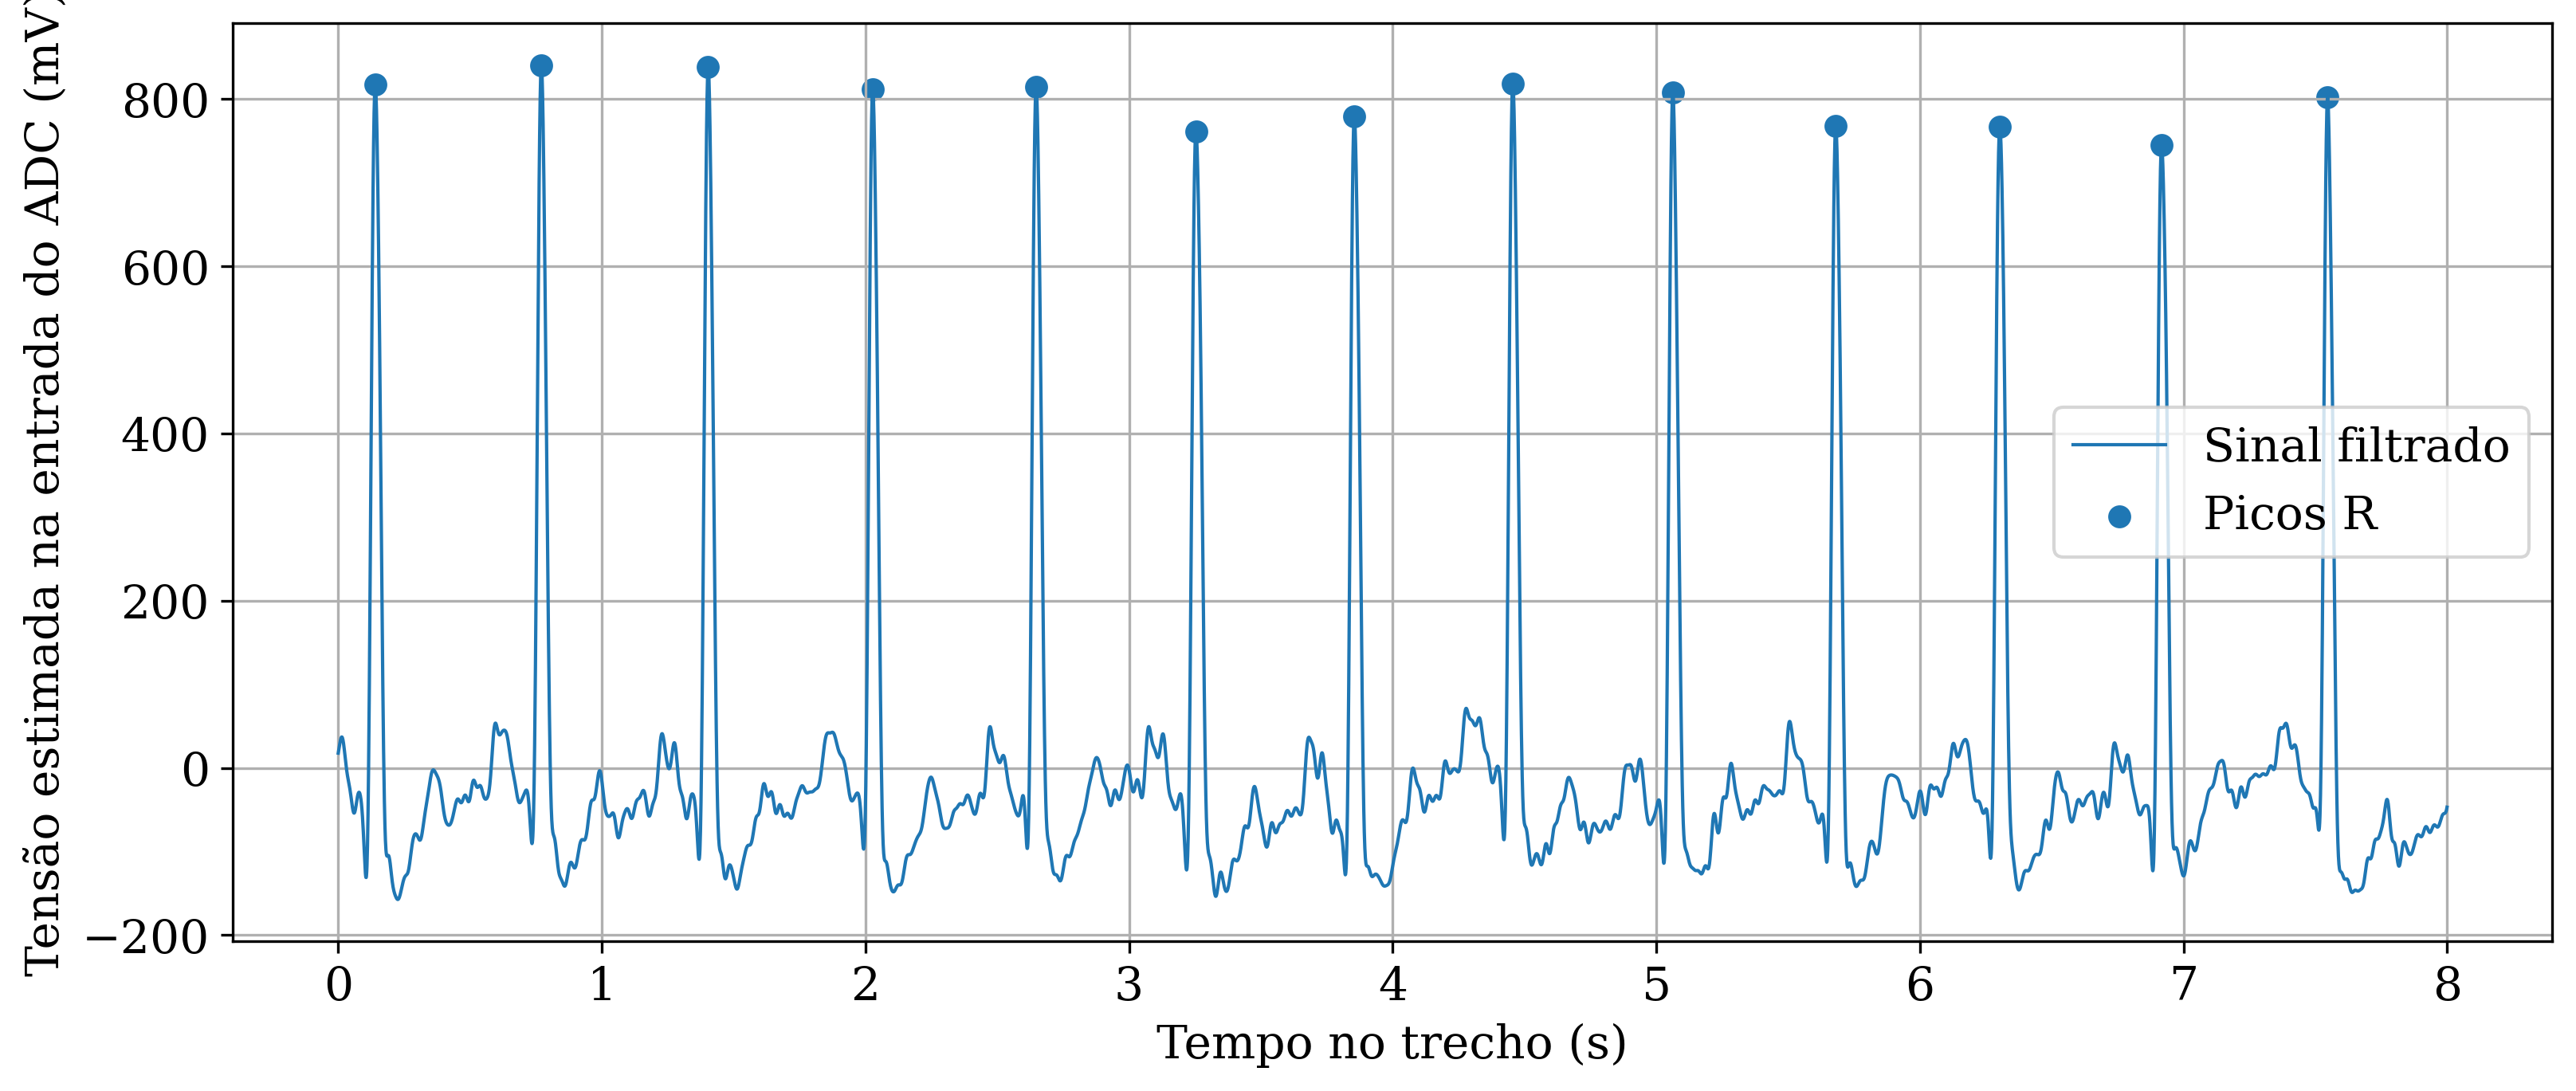
\includegraphics[width=\textwidth]{figuras/figura_ecg1_picos_r.png}
    \caption[Detecção dos picos R no primeiro canal de ECG]
    {Sinal filtrado do primeiro canal de ECG em um trecho representativo de 8~s, com a tensão estimada na entrada do conversor analógico-digital (ADC) e expressa em milivolts. Os marcadores circulares indicam os picos R identificados nos complexos QRS, utilizados como referências temporais para a análise dos ciclos cardíacos e dos intervalos entre batimentos consecutivos.}
    \label{fig:ecg1_picos}
\end{figure}

A mediana dos segmentos alinhados pelos picos R resultou no template apresentado na Figura~\ref{fig:ecg1_template}. O complexo principal apresentou amplitude pico a pico de aproximadamente 943,43~mV na entrada do ADC. Além do complexo QRS, foram encontrados candidatos morfológicos anteriores e posteriores ao evento de referência, localizados aproximadamente em $-178$~ms e $+180$~ms.

\begin{figure}[!htbp]
    \centering
    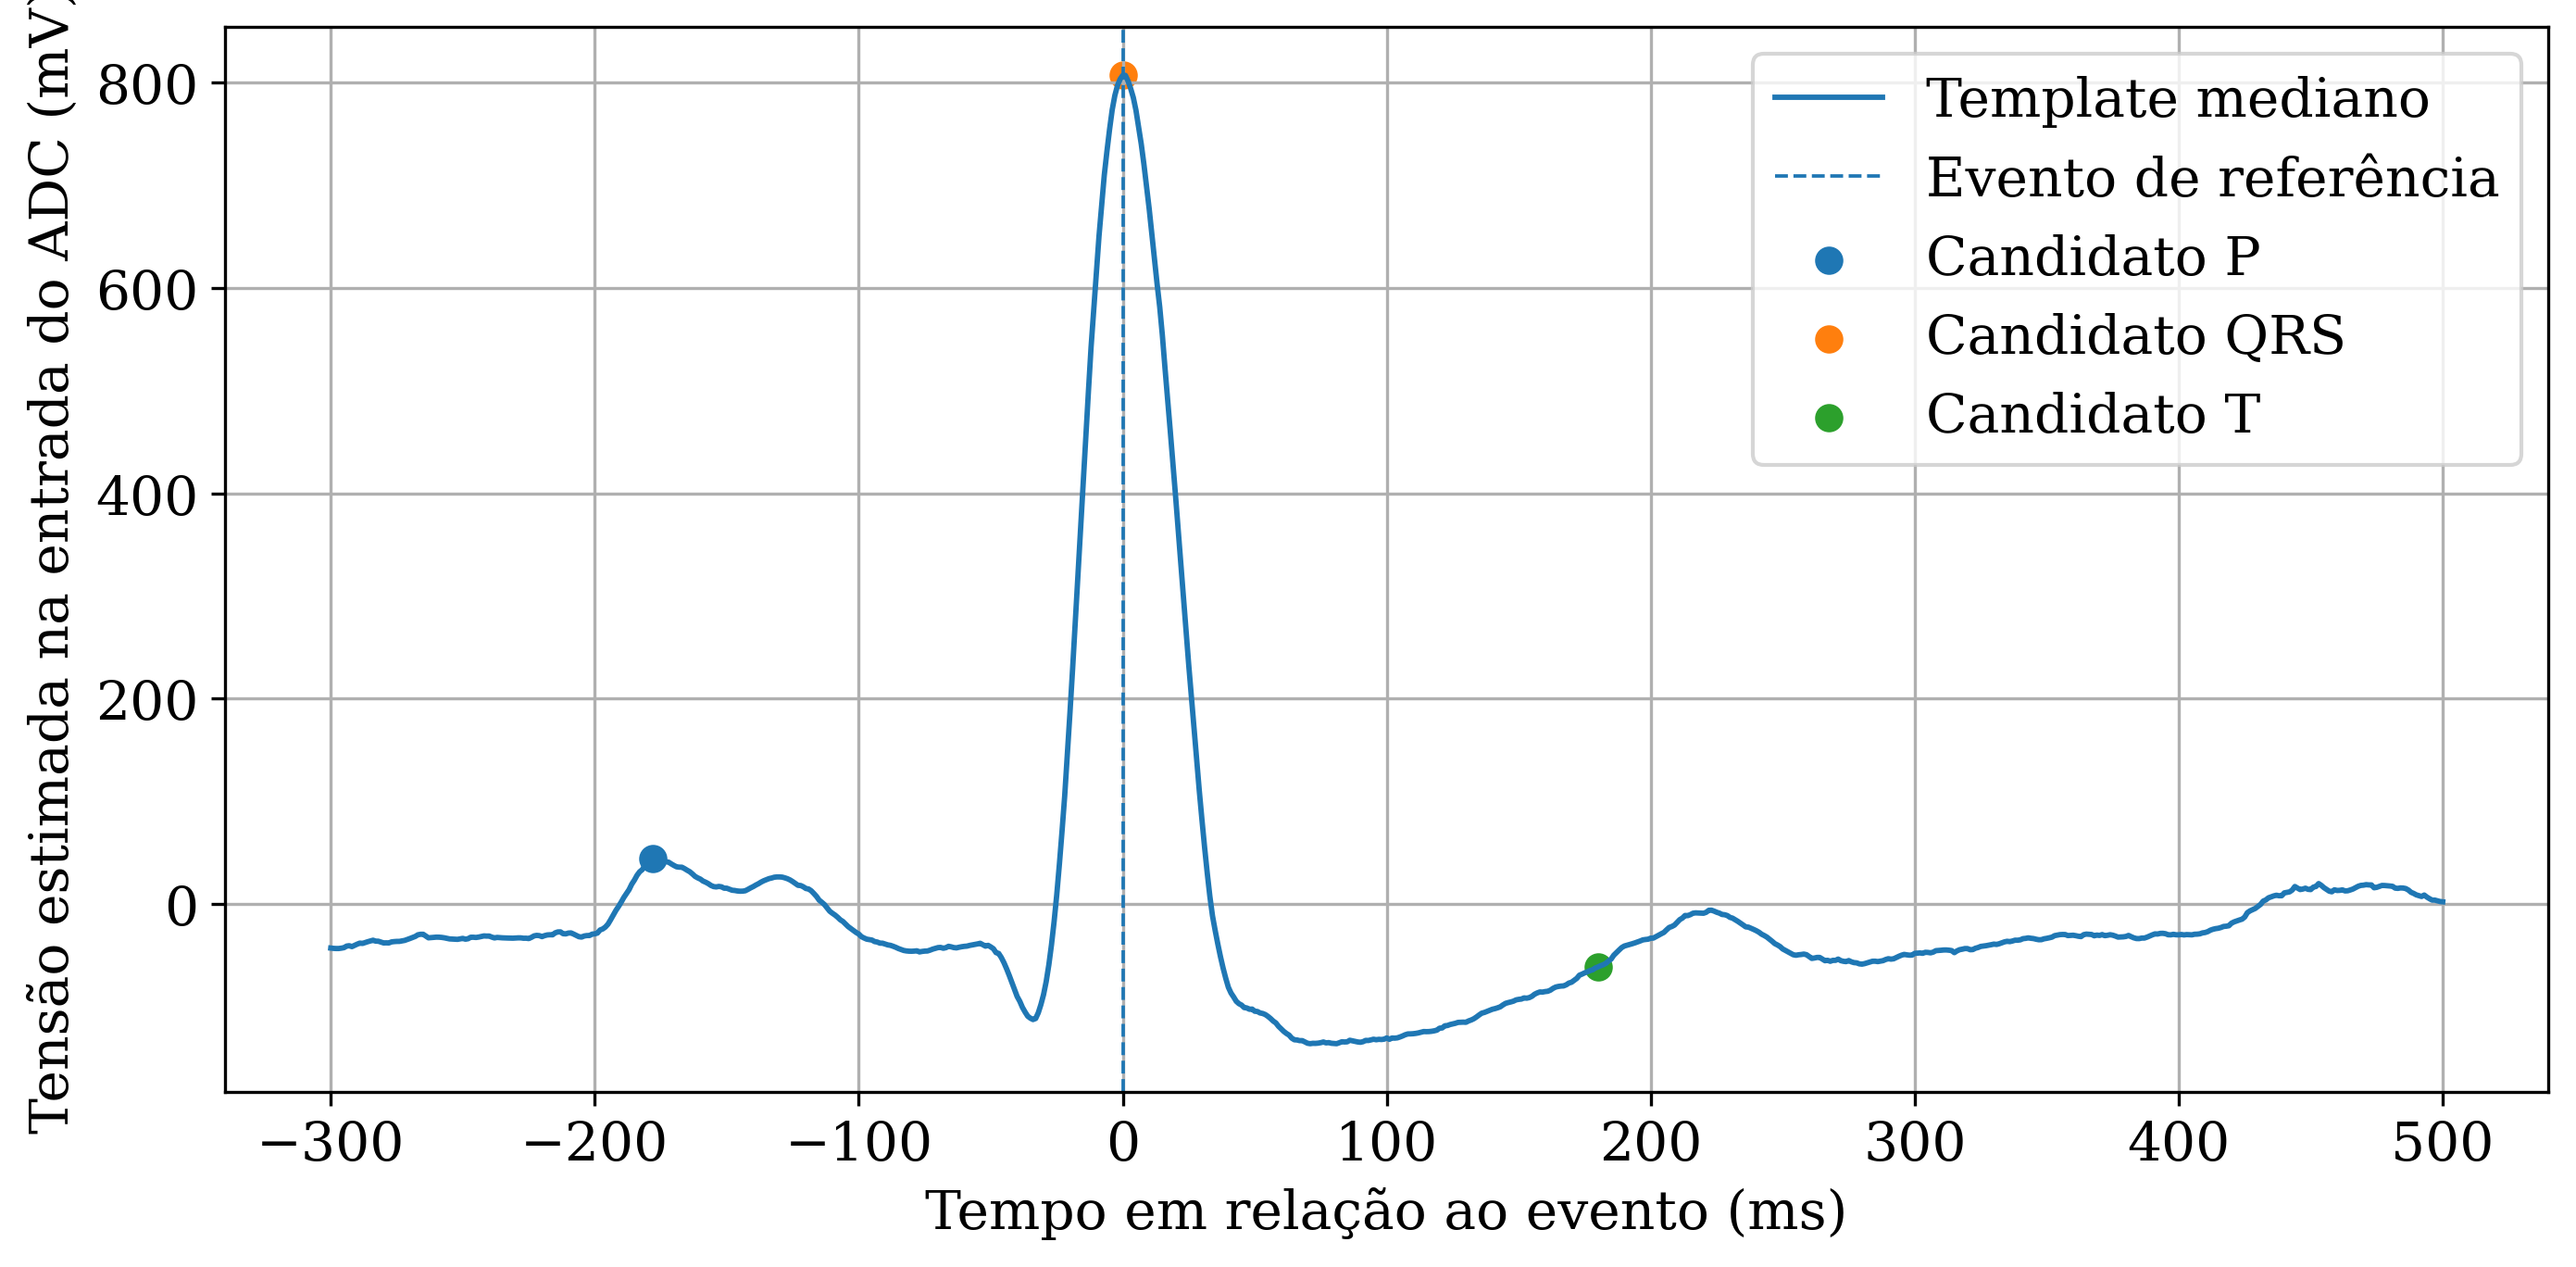
\includegraphics[width=\textwidth]{figuras/figura_ecg1_template.png}
    \caption[Template mediano do ECG~1 com candidatos às ondas cardíacas]
    {Template mediano dos ciclos cardíacos do primeiro canal de ECG, obtido após o alinhamento dos batimentos pelo pico R, definido como evento de referência em $0$~ms. A tensão estimada na entrada do conversor analógico-digital (ADC) é apresentada em milivolts. Os marcadores indicam os candidatos à onda P, ao complexo QRS e à onda T, localizados, respectivamente, antes, no instante e após o pico R.}
    \label{fig:ecg1_template}
\end{figure}

O candidato anterior ao QRS apresentou amplitude aproximada de 77,87~mV e relação com o nível de ruído de base suficiente para sua identificação pelo procedimento utilizado. O candidato posterior apresentou amplitude de aproximadamente $-27,91$~mV. Esses pontos foram interpretados apenas como estruturas morfológicas compatíveis com ondas P e T no template médio, sem atribuição de significado diagnóstico.

A linha de base apresentou variação entre os percentis de 5\% e 95\% de aproximadamente 47.285 contagens, indicando a presença de deriva lenta ao longo da sessão. Essa variação foi reduzida no sinal processado, mas permaneceu perceptível entre os complexos consecutivos.

\subsubsection{Características temporais e espectrais}
\label{subsubsec:ecg_1_metricas}

O intervalo médio entre picos R foi de 0,6306~s, enquanto a mediana foi de 0,6235~s. Esses valores corresponderam a frequências cardíacas média e mediana de 95,14 e 96,23~bpm, respectivamente. O desvio padrão dos intervalos foi de 0,0320~s e o coeficiente de variação foi de 5,07\%.

A correlação mediana entre os batimentos individuais e o template foi de 0,9947, com percentil de 5\% igual a 0,9725. Nenhum dos batimentos foi classificado como de baixa correlação pelo critério utilizado. A relação sinal-ruído calculada a partir do template foi de 16,49~dB, indicando elevada repetibilidade da morfologia média nesse canal.

A frequência dominante da densidade espectral foi de aproximadamente 4,88~Hz, enquanto a frequência mediana espectral e o centroide foram de 6,35 e 7,26~Hz. Esses valores representam a distribuição espectral da forma de onda e não devem ser confundidos com a frequência cardíaca, determinada pelos intervalos entre os picos R.

A Figura~\ref{fig:ecg1_espectro} apresenta a densidade espectral de potência do primeiro canal. A maior parte do conteúdo permaneceu concentrada abaixo de aproximadamente 40~Hz, com redução progressiva nas frequências superiores.

\begin{figure}[!htbp]
    \centering
    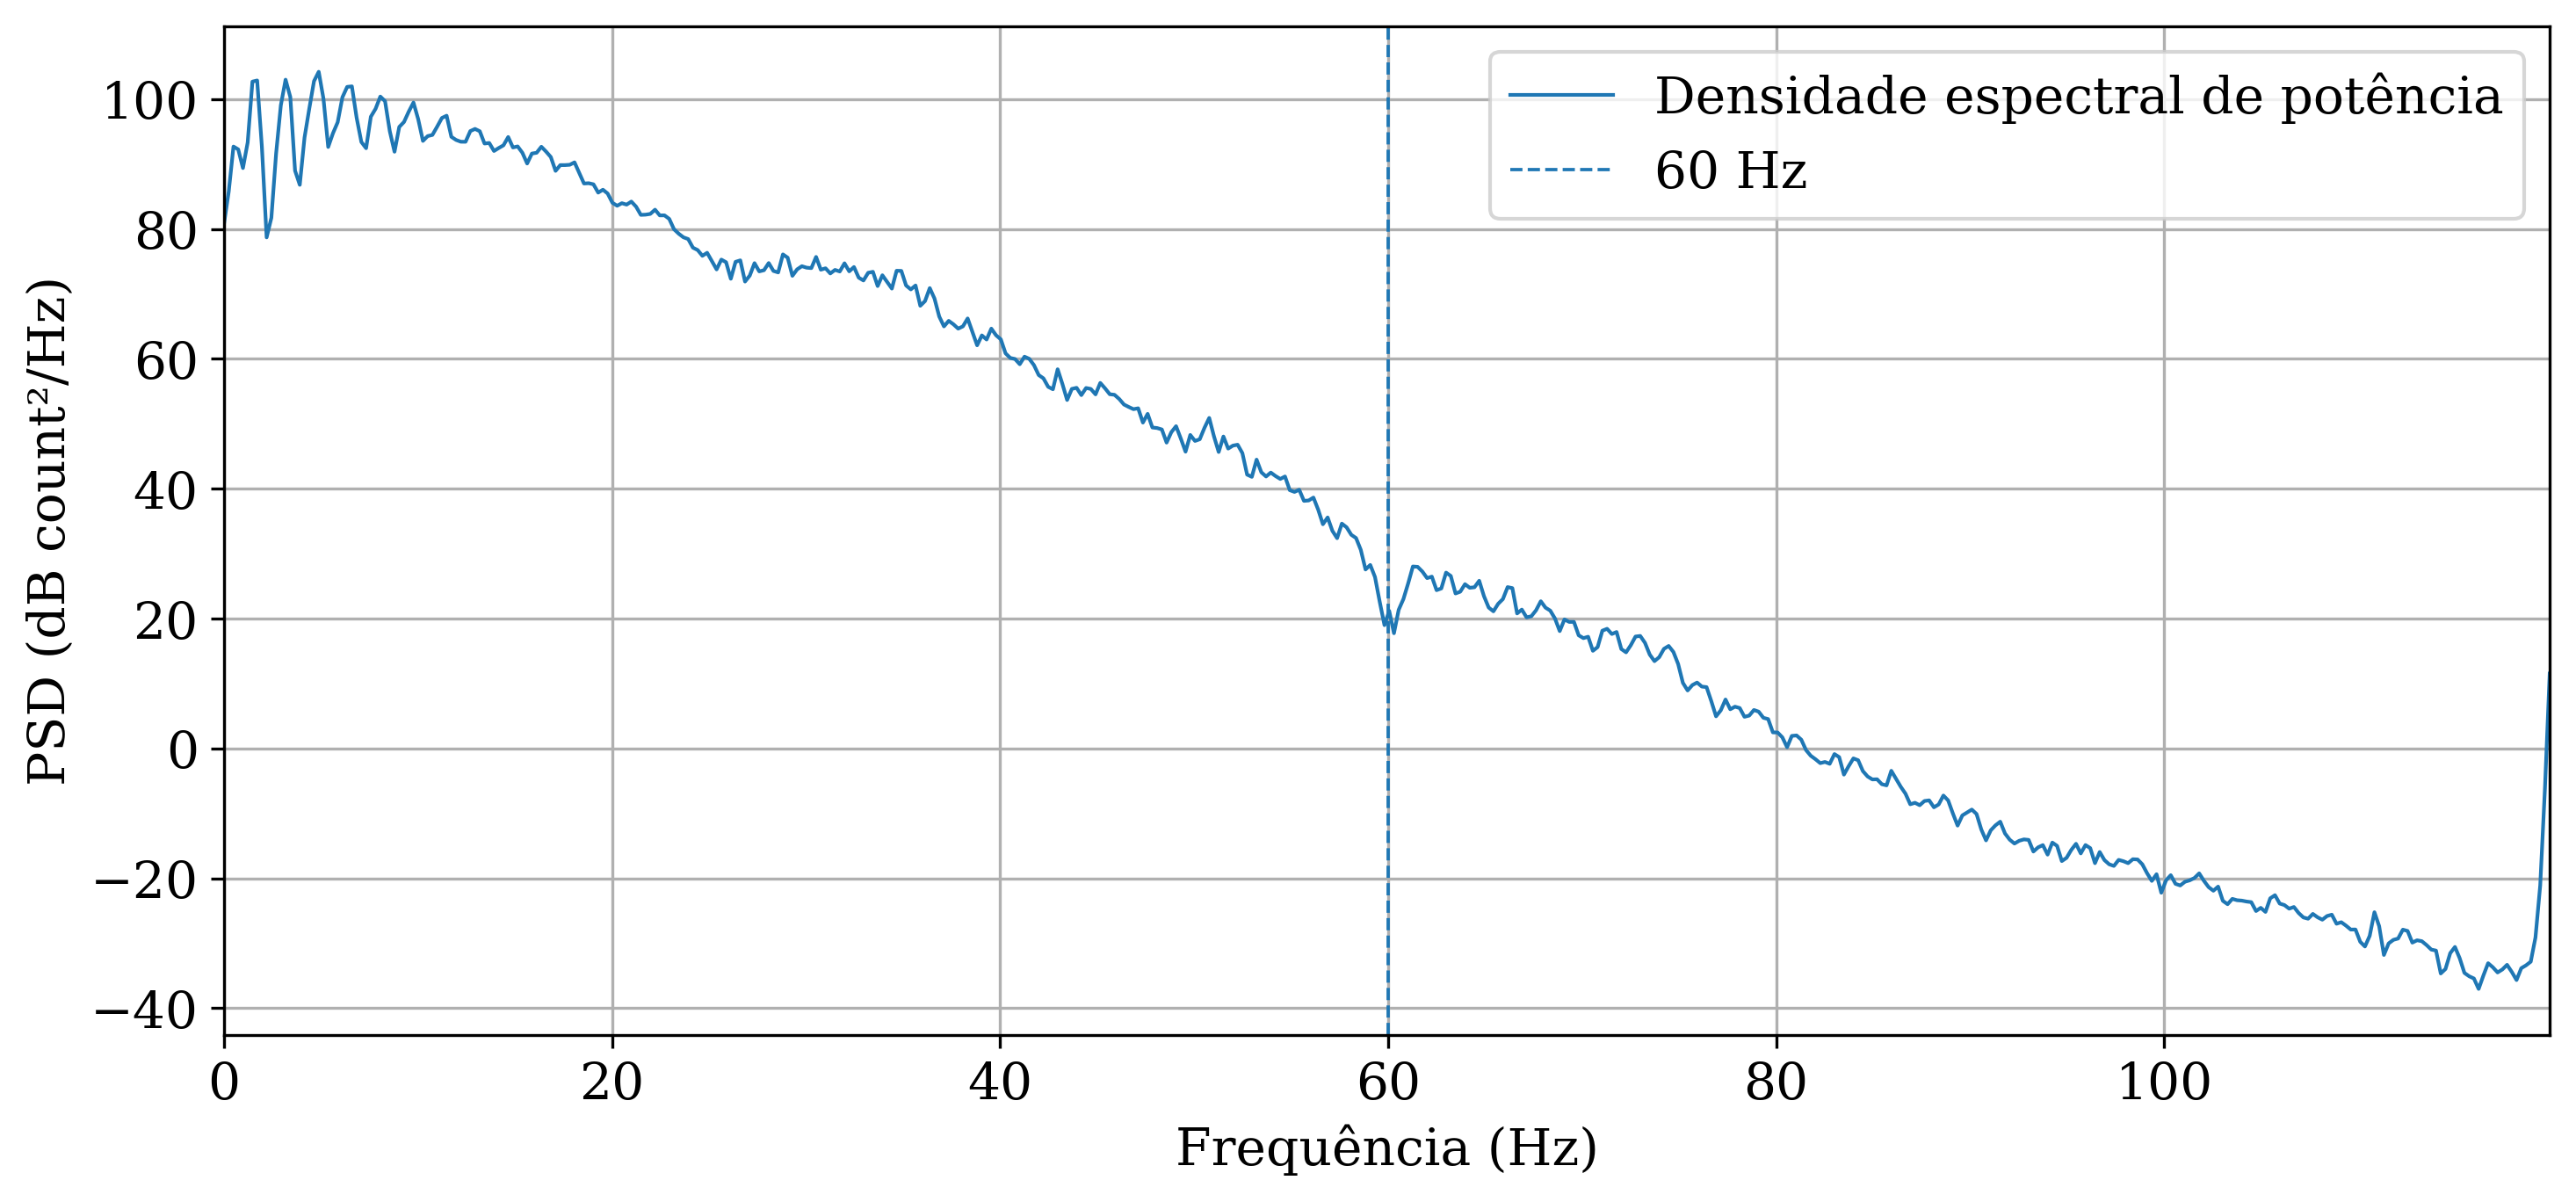
\includegraphics[width=\textwidth]{figuras/figura_ecg1_espectro.png}
    \caption[Densidade espectral de potência do ECG~1]
    {Densidade espectral de potência do primeiro canal de ECG no intervalo de 0 a 120~Hz, expressa em $\mathrm{dB\,count^2/Hz}$. A linha tracejada vertical indica a frequência de 60~Hz, associada à interferência da rede elétrica. Observa-se predominância de potência nas baixas frequências e redução progressiva do conteúdo espectral com o aumento da frequência, além de uma atenuação local nas proximidades de 60~Hz.}
    \label{fig:ecg1_espectro}
\end{figure}

A componente estimada em 60~Hz apresentou nível de $-82,89$~dB em relação ao valor eficaz do sinal filtrado. Não foi observado um pico predominante nessa frequência, indicando que a interferência da rede elétrica não constituiu a componente principal do registro analisado.

\subsubsection{Discussão do primeiro canal de ECG}
\label{subsubsec:discussao_ecg_1}

O primeiro canal apresentou a melhor relação entre amplitude, repetibilidade e separação dos eventos dentre os dois canais de ECG. Os complexos QRS foram identificados em toda a sessão, com alta correlação entre os ciclos e baixa incidência de alterações morfológicas relativas ao template.

A presença de estruturas anteriores e posteriores ao QRS no template médio foi compatível com a organização temporal esperada para um traçado eletrocardiográfico. Entretanto, como o sinal foi adquirido por um módulo de condicionamento não destinado à avaliação clínica e não foi comparado a um eletrocardiógrafo certificado, essas estruturas não foram utilizadas para estimar intervalos clínicos ou realizar interpretação diagnóstica.

A amplitude elevada correspondeu à saída condicionada do módulo AD8232 e à tensão presente na entrada do ADS1256. Dessa forma, não representa diretamente a amplitude do potencial cardíaco captado pelos eletrodos.

\subsection{Resultado do segundo canal de ECG}
\label{subsec:resultado_ecg_2}

\subsubsection{Representação no domínio do tempo}
\label{subsubsec:ecg_2_tempo}

O segundo canal também apresentou complexos de polaridade positiva sincronizados com aqueles observados no ECG~1. Foram detectados 47 picos R durante a sessão, com amplitude mediana de aproximadamente 4,73~mV na entrada do ADC. O intervalo entre os percentis de 5\% e 95\% das amplitudes foi equivalente a aproximadamente 3,44 e 5,61~mV.

A Figura~\ref{fig:ecg2_bruto_filtrado} apresenta o sinal bruto e o sinal processado. Em comparação com o primeiro canal, o ECG~2 apresentou menor amplitude e maior proporção de conteúdo irregular entre os complexos principais.

\begin{figure}[!htbp]
    \centering
    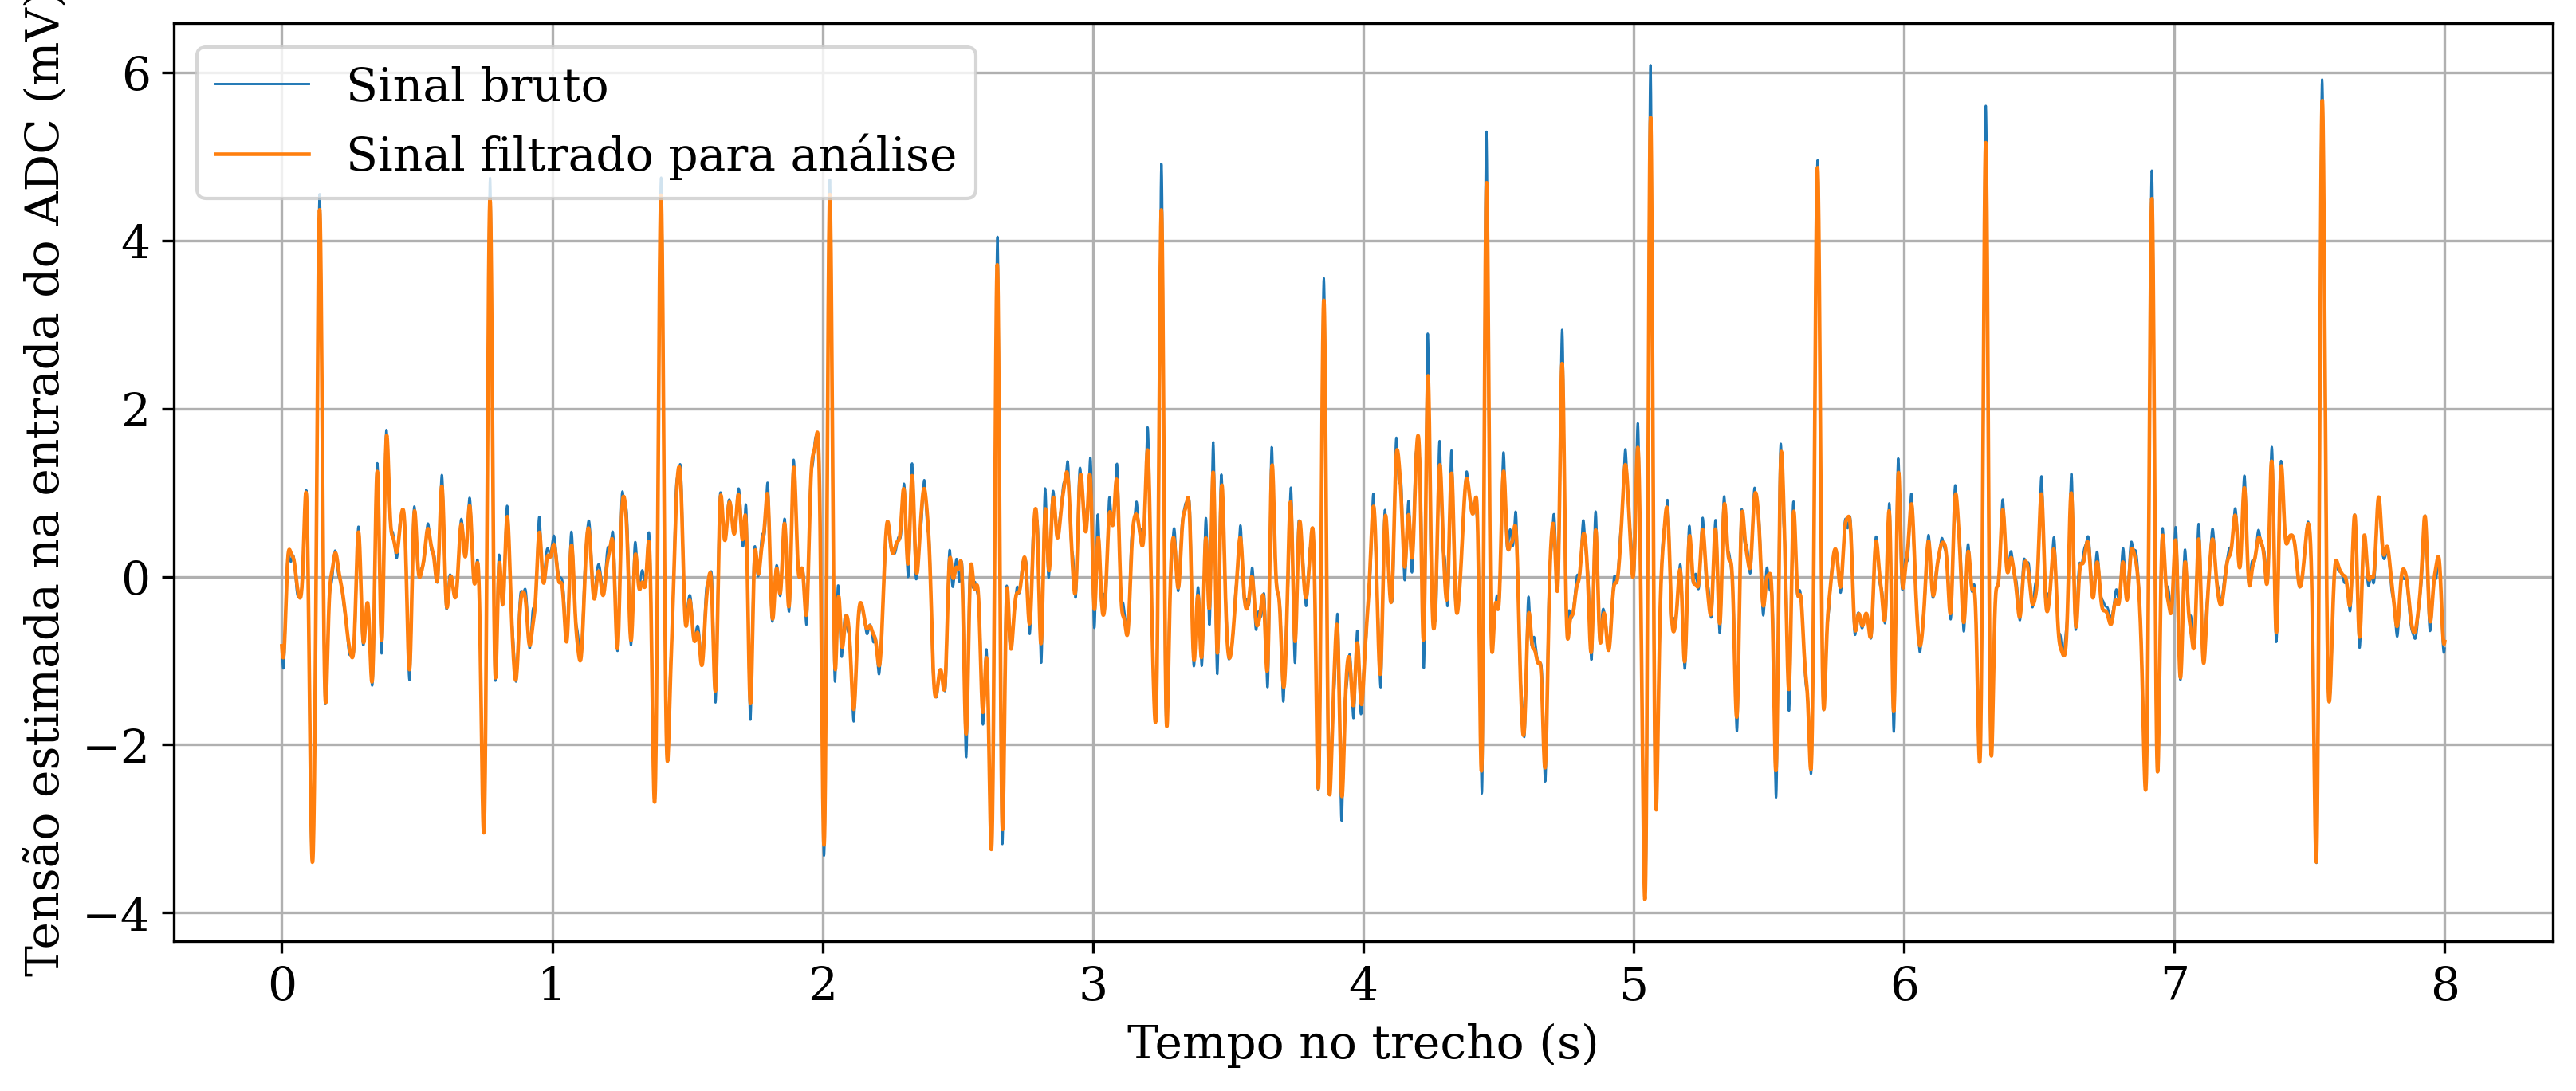
\includegraphics[width=\textwidth]{figuras/figura_ecg2_bruto_filtrado.png}
    \caption[Comparação entre os sinais bruto e filtrado do ECG~2]
    {Comparação, em um trecho representativo de 8~s, entre o sinal bruto do segundo canal de ECG e o sinal após o processamento empregado na análise. A tensão foi estimada na entrada do conversor analógico-digital (ADC) e expressa em milivolts. O sinal filtrado acompanha a evolução temporal do sinal bruto e preserva os eventos de maior amplitude, apresentando apenas pequenas alterações nas oscilações e nos valores extremos.}
    \label{fig:ecg2_bruto_filtrado}
\end{figure}

Apesar da menor relação entre os complexos e a atividade de fundo, os picos R permaneceram identificáveis, conforme apresentado na Figura~\ref{fig:ecg2_picos}. Os 13 eventos detectados no trecho representativo coincidiram temporalmente com aqueles observados no primeiro canal.

\begin{figure}[!htbp]
    \centering
    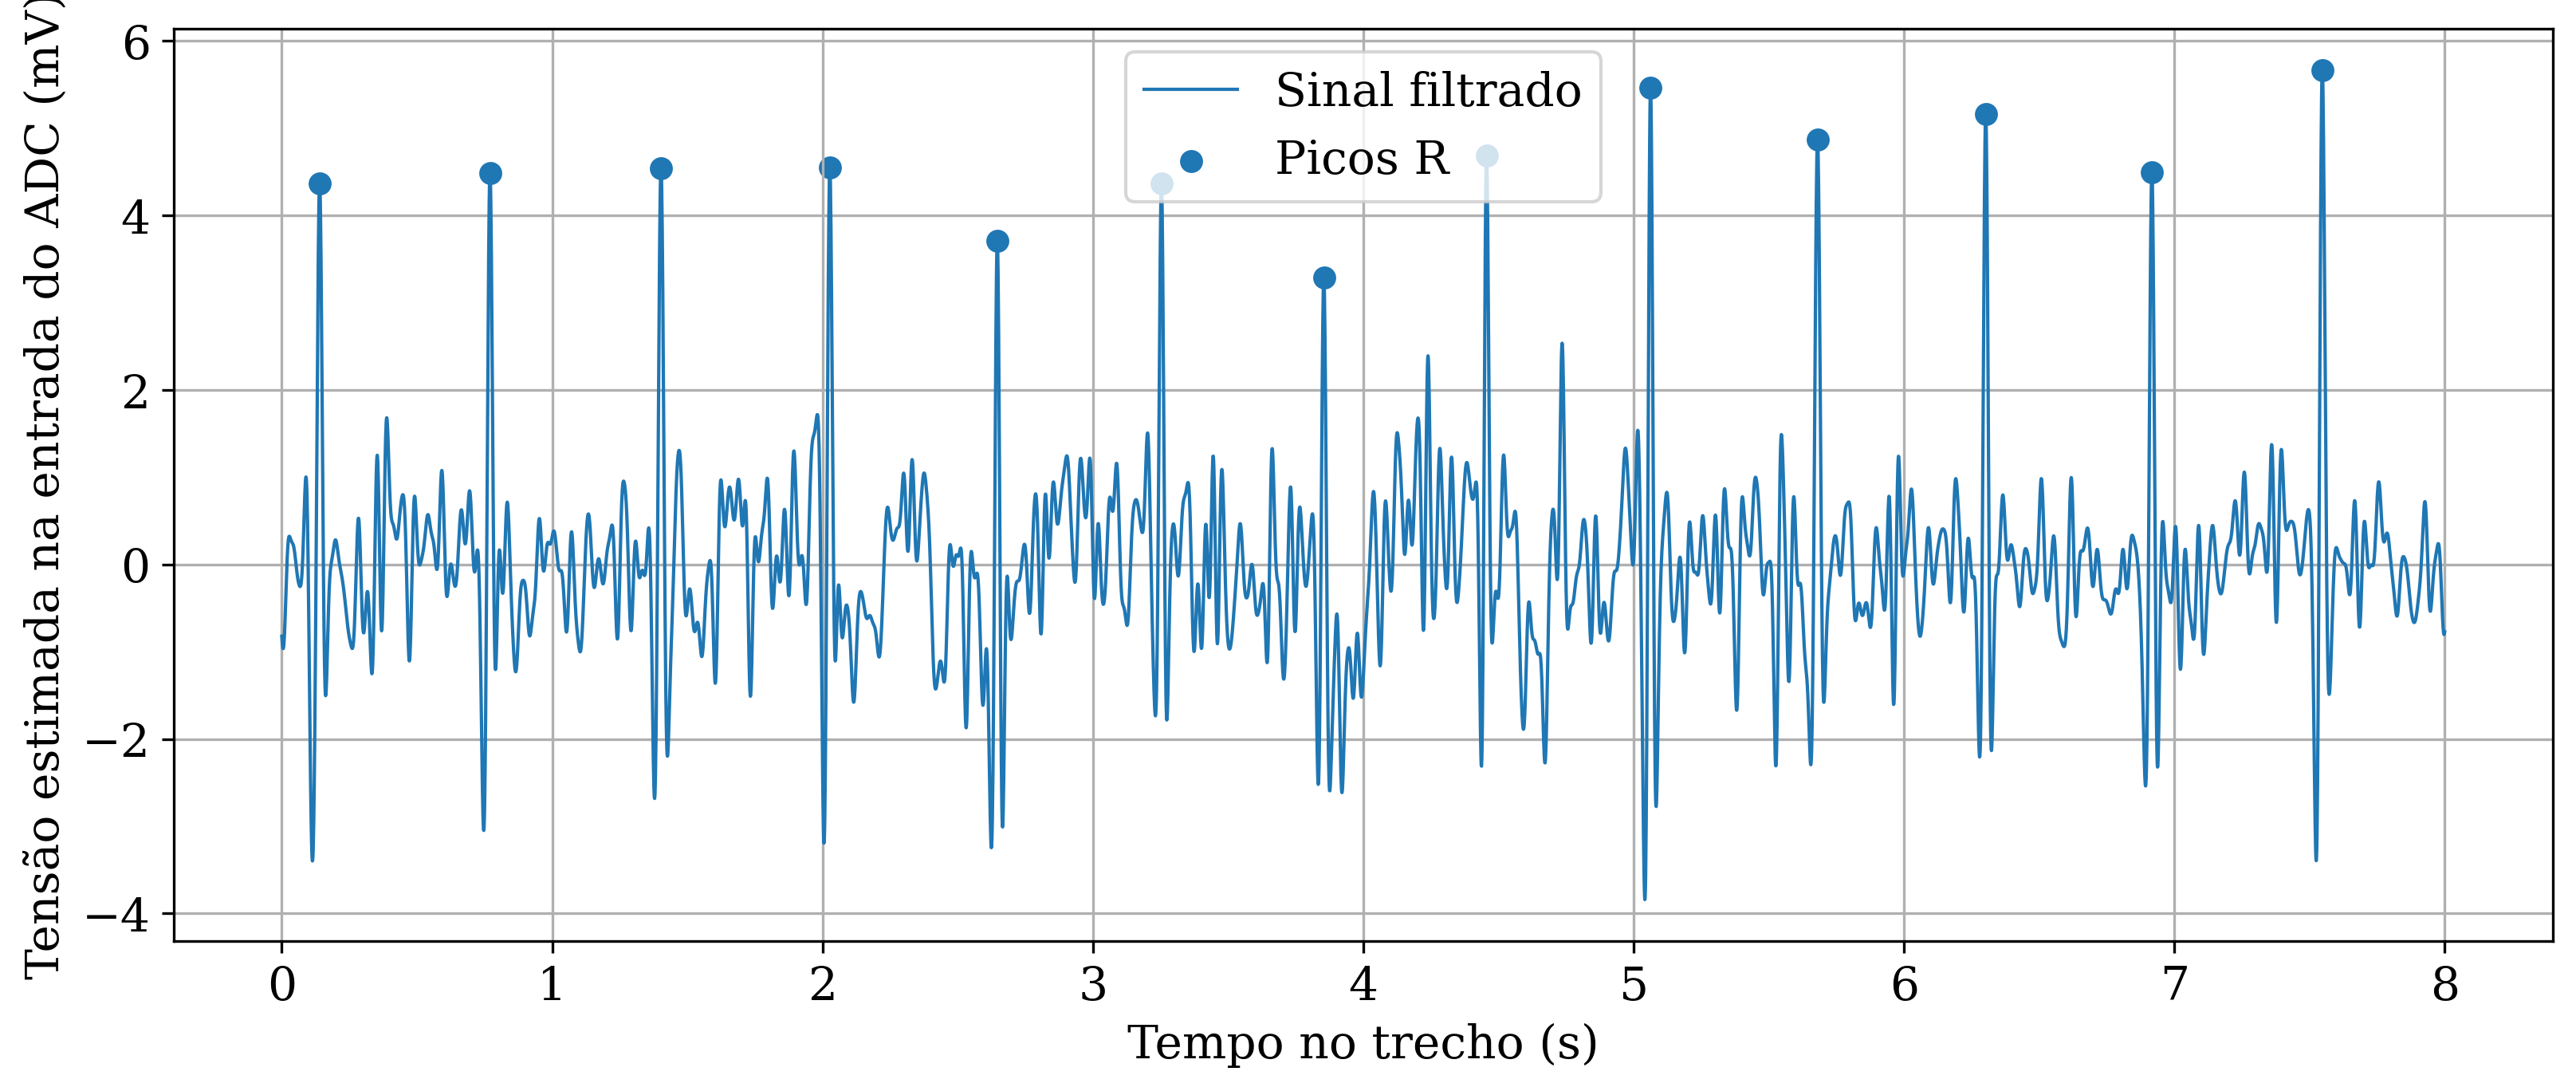
\includegraphics[width=\textwidth]{figuras/figura_ecg2_picos_r.png}
    \caption[Detecção dos picos R no segundo canal de ECG]
    {Sinal filtrado do segundo canal de ECG em um trecho representativo de 8~s, com a tensão estimada na entrada do conversor analógico-digital (ADC) e expressa em milivolts. Os marcadores circulares indicam os picos R identificados nos complexos QRS, empregados como referências temporais para a determinação dos intervalos entre batimentos consecutivos.}
    \label{fig:ecg2_picos}
\end{figure}

O template mediano do segundo canal apresentou amplitude pico a pico de aproximadamente 7,30~mV. O complexo QRS permaneceu claramente reconhecível, enquanto a estrutura anterior ao evento de referência não apresentou separação suficiente em relação ao ruído para ser classificada como uma onda P reconhecível pelo procedimento adotado. Uma estrutura posterior, localizada aproximadamente em 187~ms, apresentou comportamento compatível com um candidato à onda T.

\begin{figure}[!htbp]
    \centering
    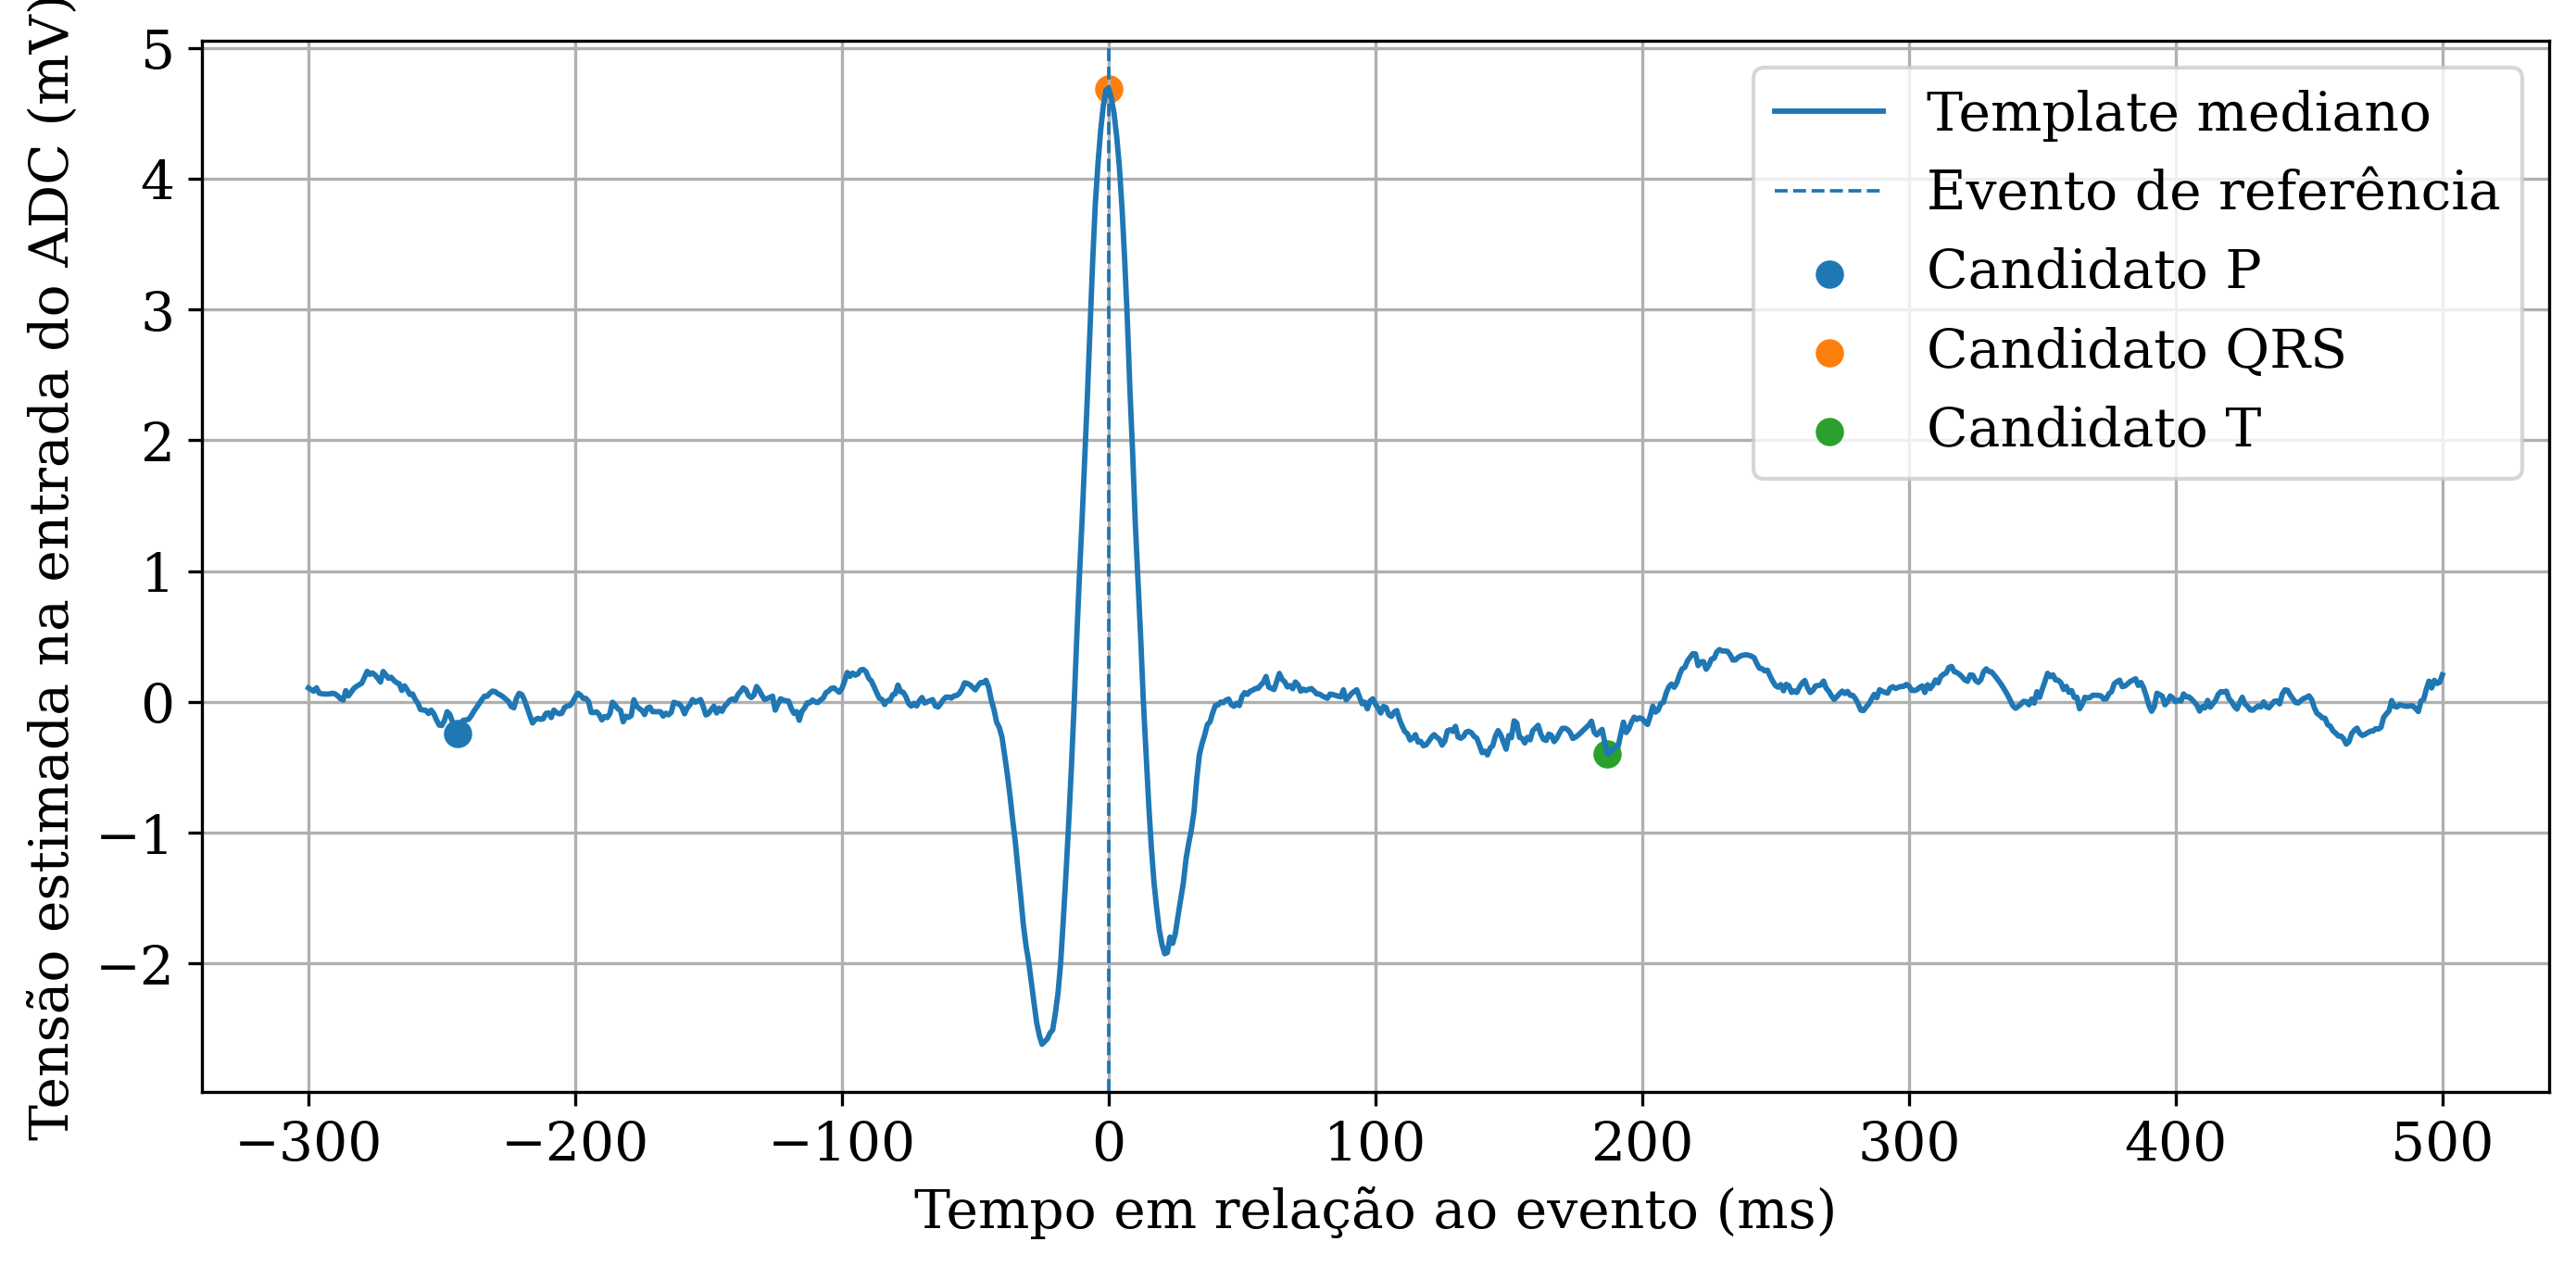
\includegraphics[width=\textwidth]{figuras/figura_ecg2_template.png}
    \caption[Template mediano do ECG~2 com candidatos morfológicos]
    {Template mediano dos ciclos cardíacos do segundo canal de ECG, obtido pelo alinhamento dos batimentos em relação ao pico R, definido como evento de referência. Os marcadores indicam os candidatos morfológicos associados à onda P, ao complexo QRS e à onda T, permitindo caracterizar sua posição temporal e amplitude no ciclo cardíaco representativo.}
    \label{fig:ecg2_template}
\end{figure}

A menor amplitude do segundo canal não deve ser interpretada diretamente como redução da atividade cardíaca. Os dois registros foram obtidos por cadeias de condicionamento e posicionamentos de eletrodos independentes, podendo apresentar ganhos, orientações e sensibilidades distintas.

\subsubsection{Características temporais e espectrais}
\label{subsubsec:ecg_2_metricas}

O intervalo médio entre picos R foi de 0,6306~s, com mediana de 0,6240~s. As frequências cardíacas média e mediana foram de 95,15 e 96,15~bpm, respectivamente. O desvio padrão dos intervalos foi de 0,0319~s e o coeficiente de variação foi de 5,06\%.

A correlação mediana dos batimentos com o template foi de 0,7859, com percentil de 5\% igual a 0,5817. Aproximadamente 17,78\% dos batimentos foram classificados como de baixa correlação, e a relação sinal-ruído do template foi de 1,37~dB. Esses valores confirmaram menor repetibilidade morfológica e maior influência do ruído em comparação com o primeiro canal.

A frequência dominante da densidade espectral foi de aproximadamente 14,16~Hz, enquanto a frequência mediana espectral foi de 17,82~Hz e o centroide correspondeu a 17,64~Hz. A maior concentração em frequências intermediárias e altas foi coerente com a presença mais acentuada de oscilações rápidas no registro.

A Figura~\ref{fig:ecg2_espectro} apresenta a densidade espectral de potência do segundo canal. A redução da potência ocorreu de forma mais gradual do que no ECG~1, indicando maior participação relativa de componentes de frequência intermediária.

\begin{figure}[!htbp]
    \centering
    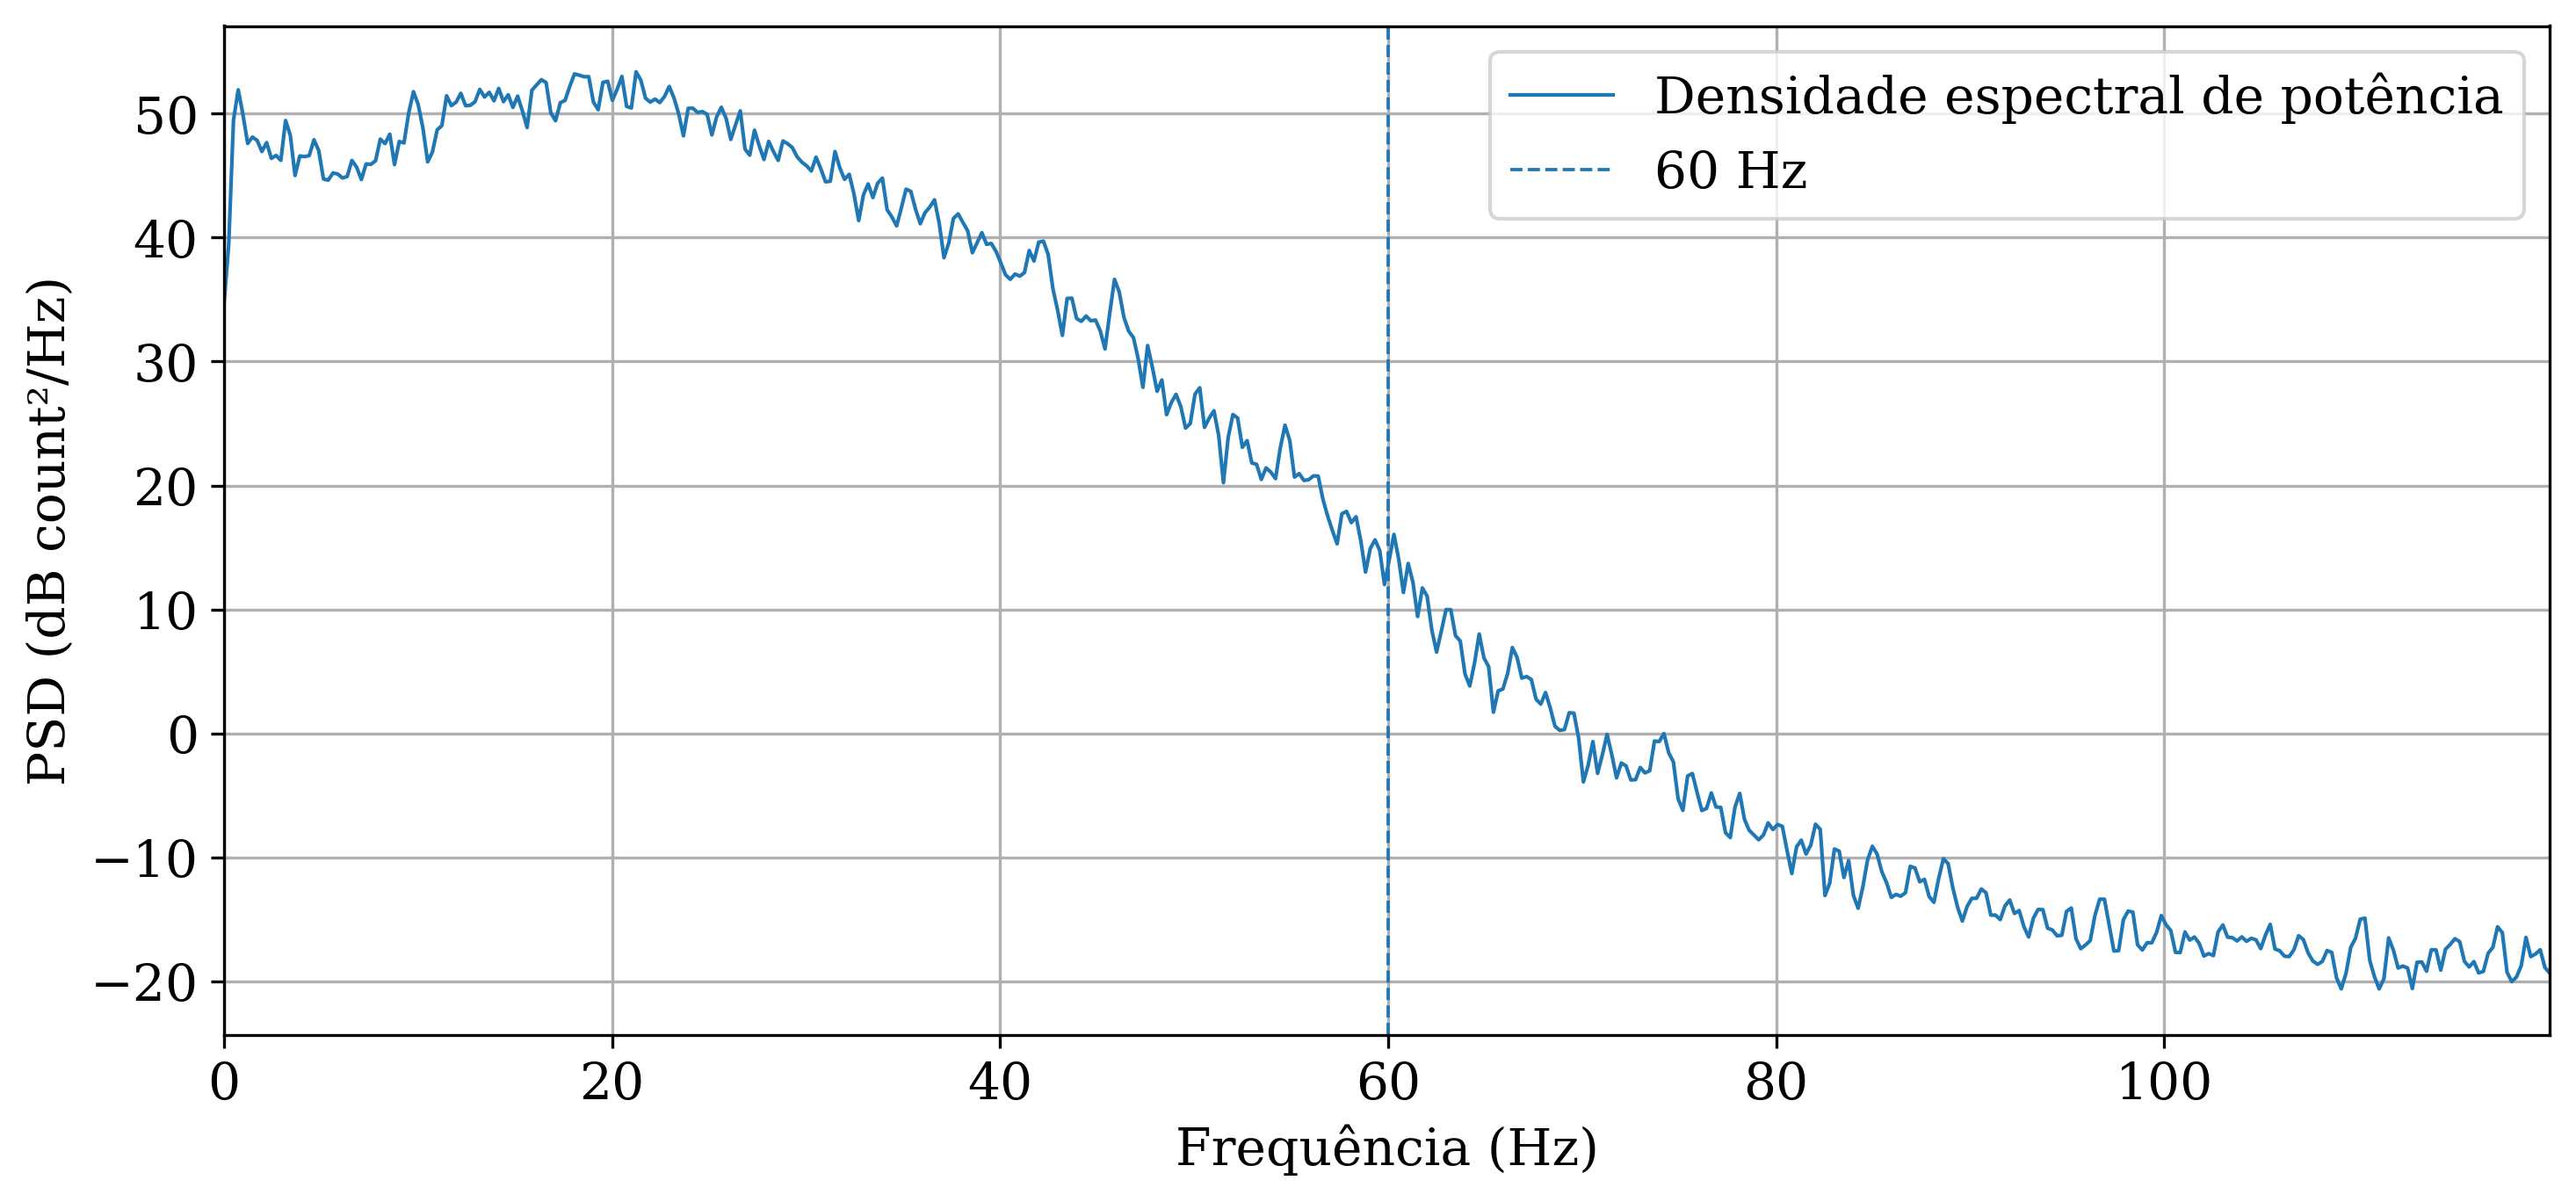
\includegraphics[width=\textwidth]{figuras/figura_ecg2_espectro.png}
    \caption[Densidade espectral de potência do ECG~2]
    {Densidade espectral de potência do segundo canal de ECG no intervalo de 0 a 120~Hz, expressa em $\mathrm{dB\,count^2/Hz}$. A linha tracejada vertical indica a frequência de 60~Hz, utilizada como referência para a avaliação de interferência proveniente da rede elétrica. Observa-se maior concentração de potência nas baixas frequências e redução progressiva do conteúdo espectral com o aumento da frequência.}
    \label{fig:ecg2_espectro}
\end{figure}

A componente estimada em 60~Hz apresentou nível de $-64,13$~dB em relação ao valor eficaz do sinal filtrado. Embora esse nível tenha sido superior ao observado no ECG~1, a frequência de 60~Hz não constituiu o pico dominante do espectro.

\subsubsection{Comparação entre os dois canais de ECG}
\label{subsubsec:comparacao_ecg}

Os dois canais apresentaram 47 picos R, todos associados entre si pelo critério de correspondência temporal. O atraso mediano do ECG~2 em relação ao ECG~1 foi de 0~ms, assim como o erro absoluto mediano de alinhamento. As frequências cardíacas médias diferiram em apenas 0,0033~bpm, correspondente a aproximadamente 0,0034\%.

A Figura~\ref{fig:comparacao_templates_ecg} apresenta os templates normalizados e alinhados pelo pico R. A coincidência temporal do evento principal é evidente, embora as formas ao redor do complexo apresentem diferenças de amplitude relativa, largura e polaridade das deflexões secundárias.

\begin{figure}[!htbp]
    \centering
    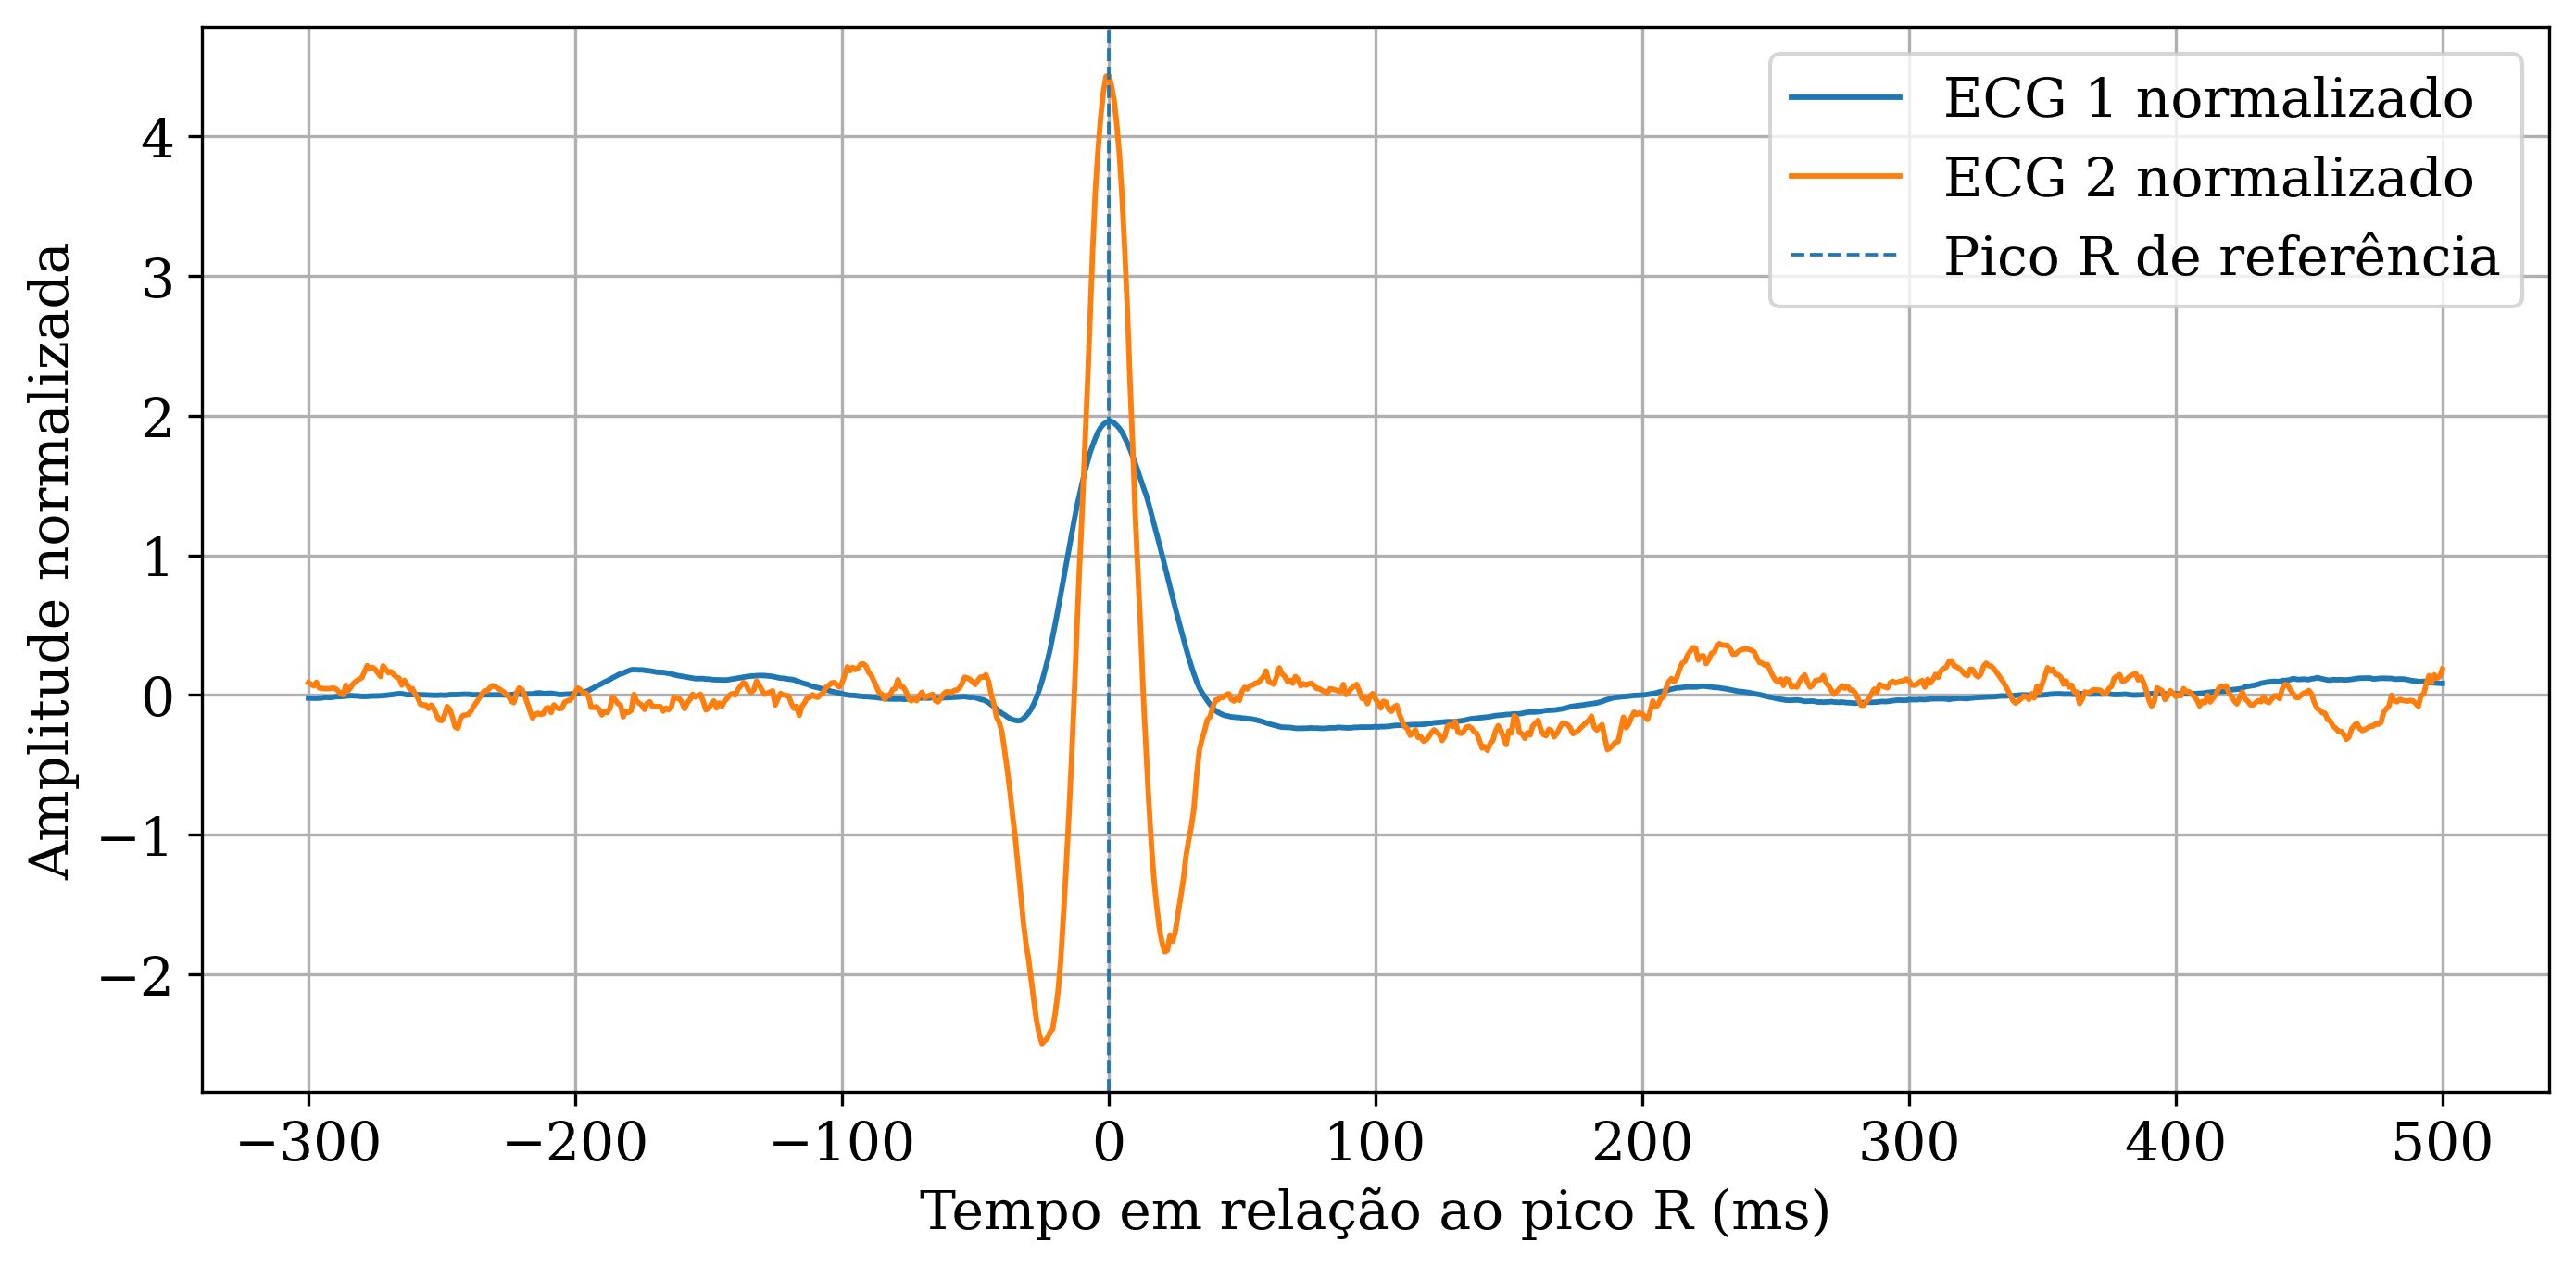
\includegraphics[width=\textwidth]{figuras/figura_comparacao_templates_ecg.png}
    \caption[Comparação dos templates normalizados dos canais de ECG]
    {Comparação dos templates normalizados dos canais ECG~1 e ECG~2 no intervalo de $-300$ a $500$~ms, obtidos a partir dos ciclos cardíacos representativos e alinhados pelo pico R. A linha tracejada vertical em $0$~ms indica o pico R de referência, permitindo comparar a morfologia, a polaridade e a distribuição temporal das componentes dos dois sinais em torno do complexo QRS.}
    \label{fig:comparacao_templates_ecg}
\end{figure}

A correlação entre os templates normalizados foi de 0,5101, indicando correspondência temporal do complexo principal, mas sem elevada semelhança morfológica global. O primeiro canal apresentou relação sinal-ruído de 16,49~dB, enquanto o segundo apresentou 1,37~dB. A amplitude mediana dos picos R na entrada do ADC foi aproximadamente 169,6 vezes maior no ECG~1.

Essas diferenças podem estar associadas ao posicionamento dos eletrodos, à orientação da derivação, às características individuais dos módulos AD8232 e às conexões utilizadas. Como as amplitudes correspondem às saídas condicionadas, não foi realizada comparação fisiológica direta entre seus valores absolutos.

Funcionalmente, os dois canais registraram os mesmos eventos cardíacos e produziram estimativas praticamente idênticas da frequência cardíaca. O ECG~1 apresentou melhor repetibilidade morfológica, enquanto o ECG~2 demonstrou que eventos cardíacos ainda podiam ser detectados em um canal de menor amplitude e maior conteúdo de ruído.

\subsection{Resultado do canal de PPG}
\label{subsec:resultado_ppg}

\subsubsection{Representação no domínio do tempo}
\label{subsubsec:ppg_tempo}

O sinal de PPG apresentou oscilações pulsáteis positivas e periódicas, com amplitude mediana de pulso de aproximadamente 50,32~mV na entrada do ADC. Foram identificados 47 picos ao longo da sessão, correspondentes ao mesmo número de eventos detectados nos canais de ECG.

A Figura~\ref{fig:ppg_bruto_filtrado} apresenta o sinal bruto e o sinal utilizado na análise. O processamento reduziu a variação lenta da linha de base e preservou os máximos pulsáteis empregados na determinação dos intervalos entre pulsos.

\begin{figure}[!htbp]
    \centering
    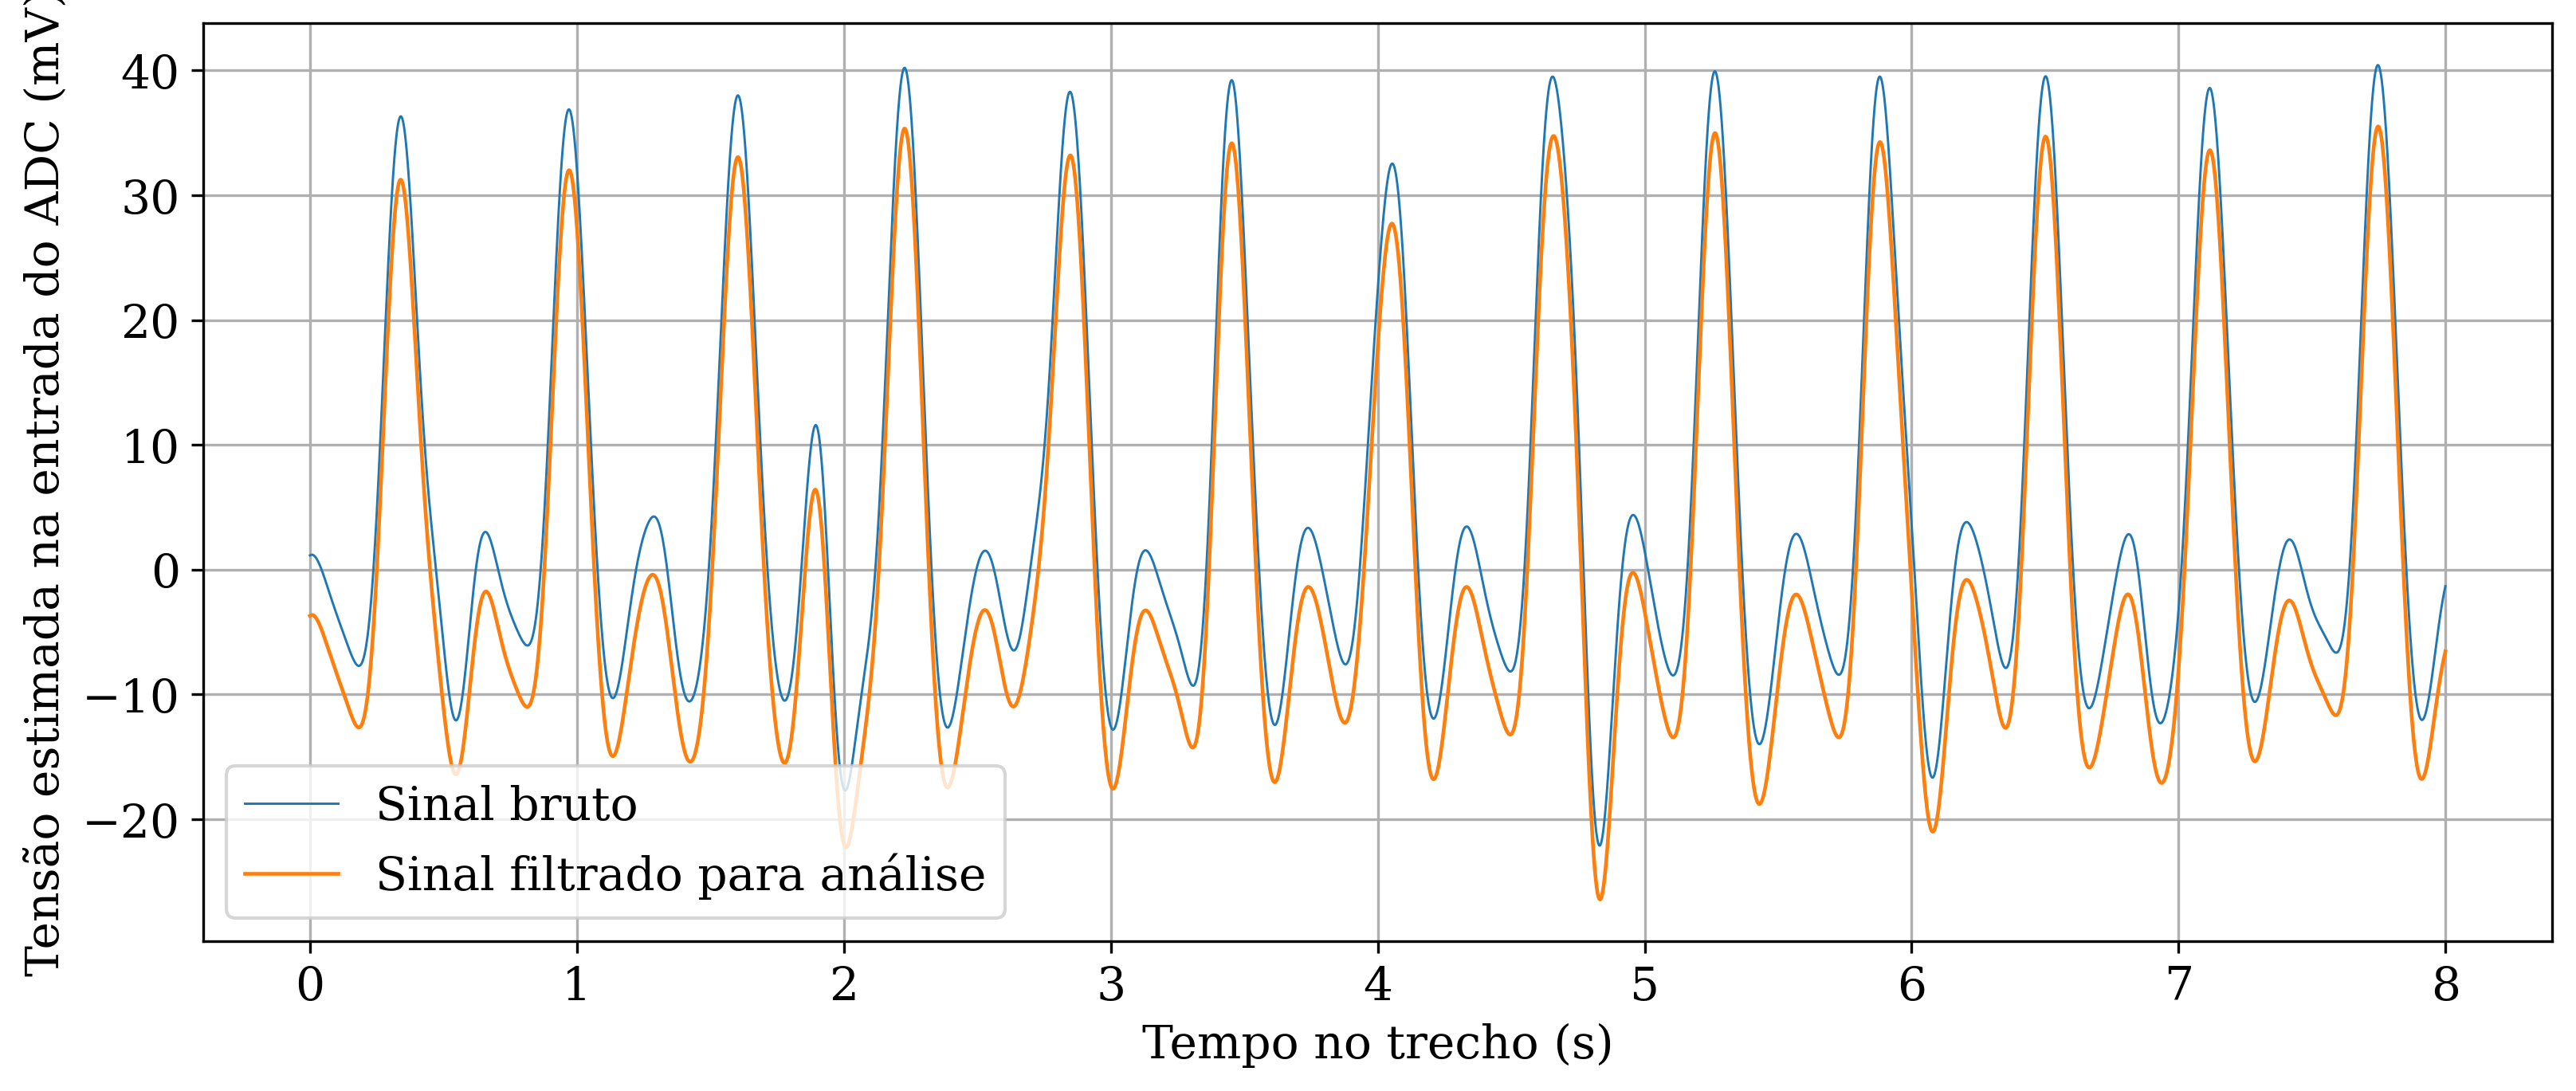
\includegraphics[width=\textwidth]{figuras/figura_ppg_bruto_filtrado.png}
    \caption[Comparação entre os sinais bruto e filtrado de PPG]
    {Comparação, em um trecho representativo de 8~s, entre o sinal bruto de fotopletismografia (PPG) e o sinal resultante do processamento empregado na análise. A tensão foi estimada na entrada do conversor analógico-digital (ADC) e expressa em milivolts. O sinal filtrado preserva a periodicidade e a posição temporal dos pulsos do sinal bruto, ao mesmo tempo que modifica seu nível de base e atenua parte das variações de menor interesse para a análise.}
    \label{fig:ppg_bruto_filtrado}
\end{figure}

Os picos identificados no trecho representativo são apresentados na Figura~\ref{fig:ppg_picos}. A maior parte dos pulsos apresentou amplitude e espaçamento semelhantes, embora tenham sido observadas variações locais em alguns ciclos.

\begin{figure}[!htbp]
    \centering
    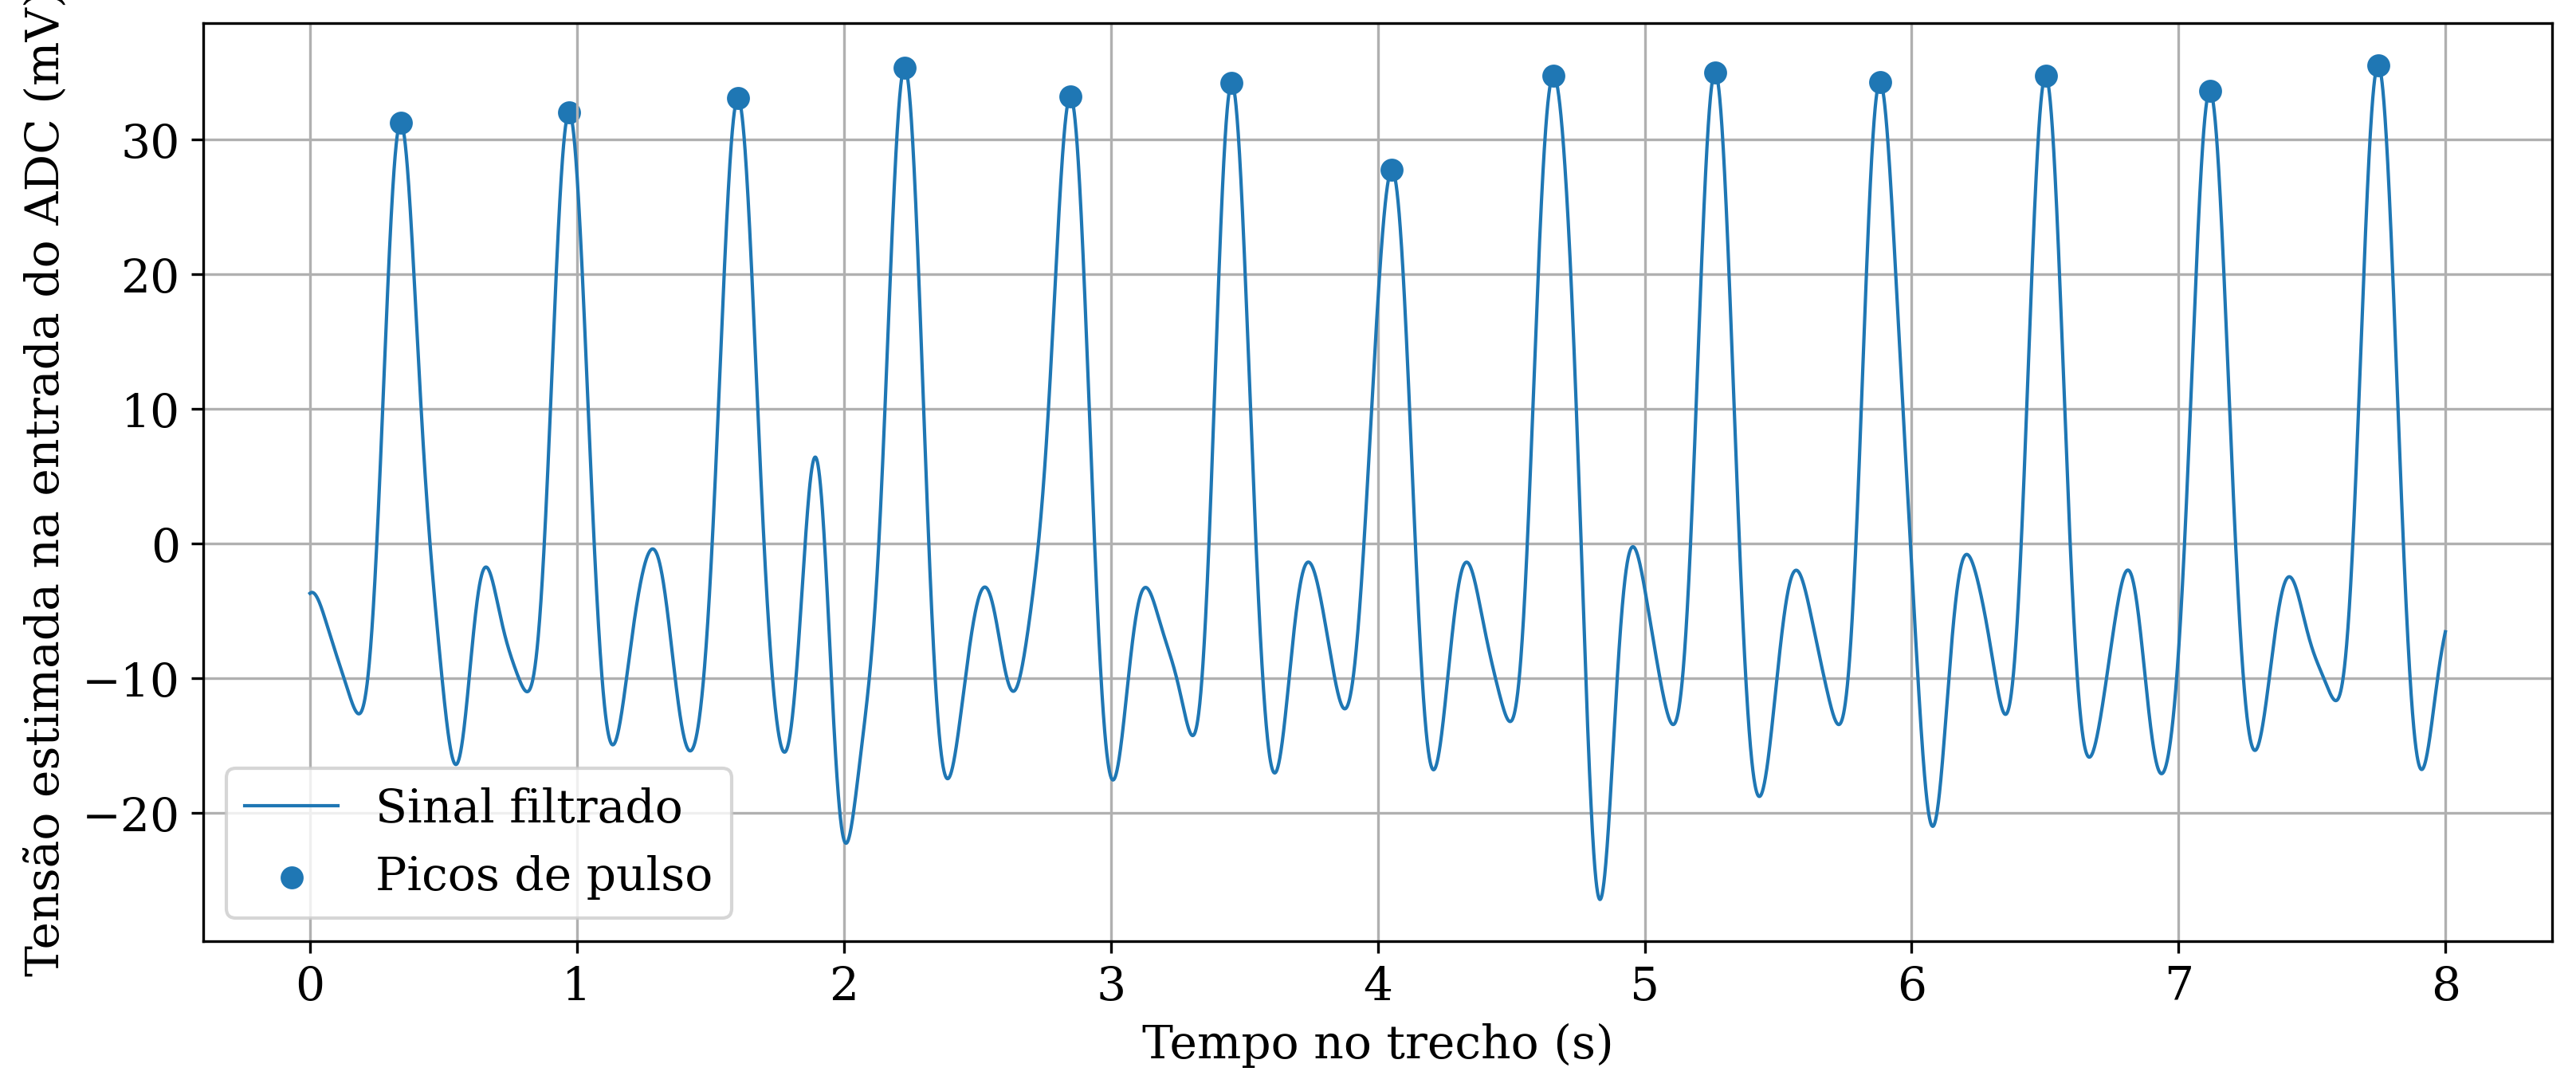
\includegraphics[width=\textwidth]{figuras/figura_ppg_picos.png}
    \caption[Detecção dos picos de pulso no sinal de PPG]
    {Sinal filtrado de fotopletismografia (PPG) em um trecho representativo de 8~s, com a tensão estimada na entrada do conversor analógico-digital (ADC) e expressa em milivolts. Os marcadores circulares indicam os picos de pulso identificados, utilizados como referências temporais para a determinação dos intervalos entre pulsos consecutivos e a estimativa da frequência cardíaca.}
    \label{fig:ppg_picos}
\end{figure}

O coeficiente de variação da amplitude pulsátil foi de 12,59\%, indicando maior variabilidade de amplitude do que aquela observada nos intervalos temporais. Essa variação pode estar relacionada à pressão de contato, ao movimento do sensor, à perfusão local ou à iluminação incidente. O registro isolado não permite separar quantitativamente essas causas.

O template mediano, apresentado na Figura~\ref{fig:ppg_template}, preservou um máximo principal largo e oscilações posteriores de menor amplitude. Essa forma foi consistente com a natureza pulsátil do sinal óptico adquirido.

\begin{figure}[!htbp]
    \centering
    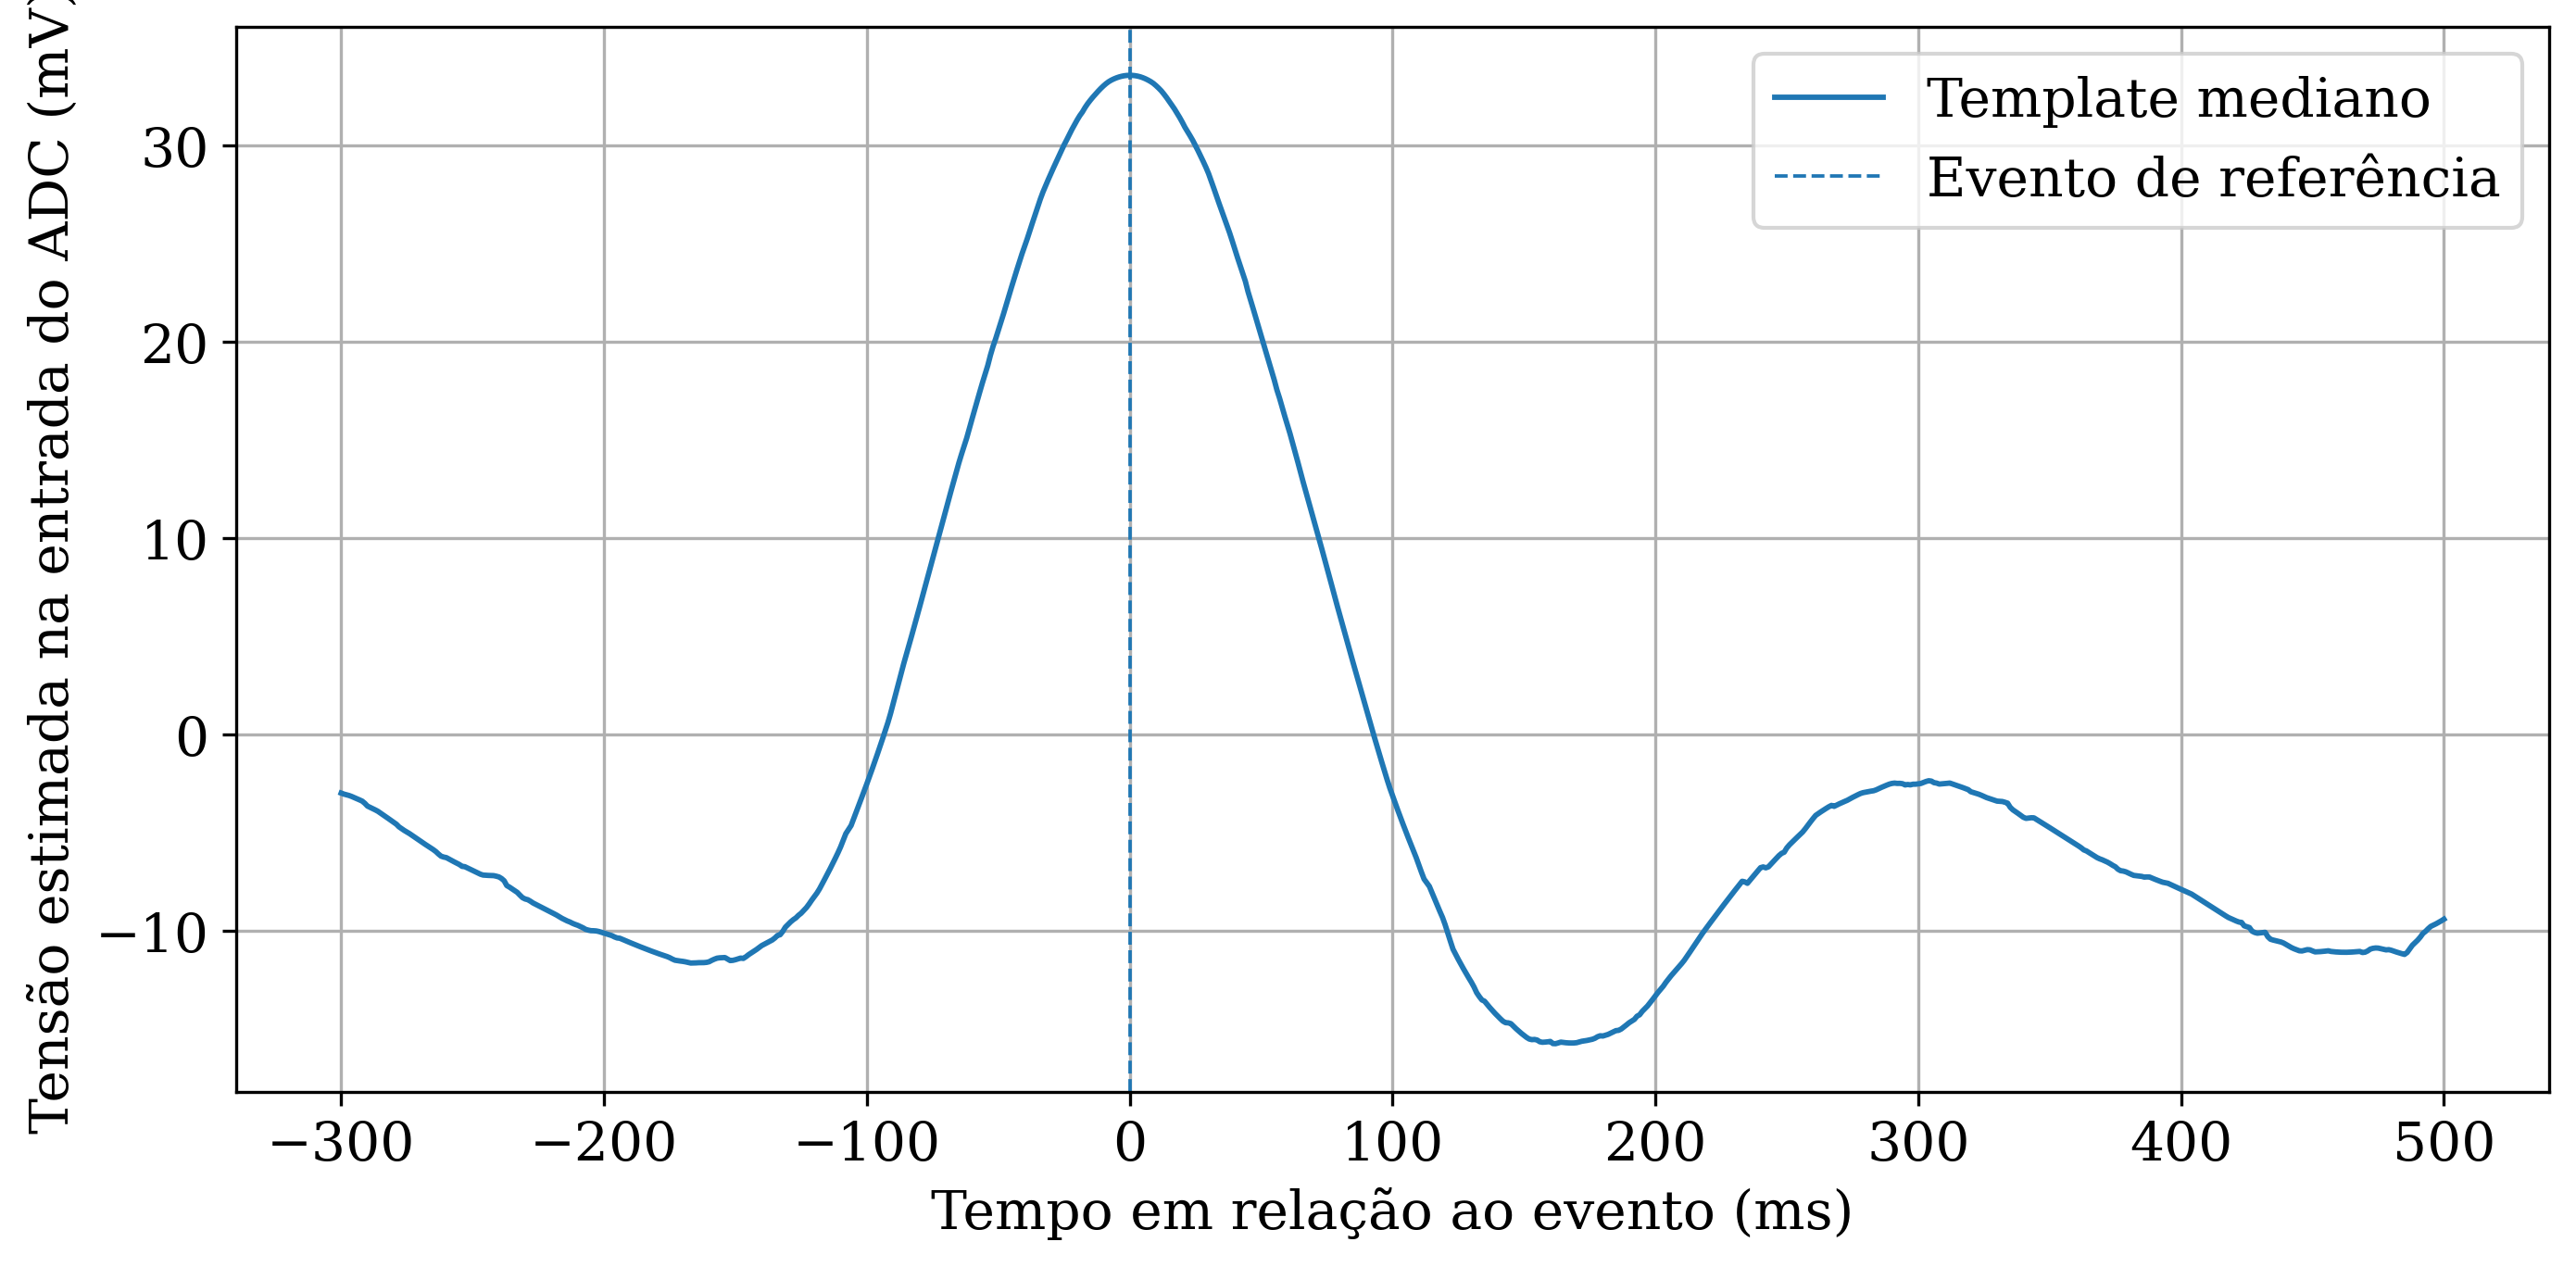
\includegraphics[width=\textwidth]{figuras/figura_ppg_template.png}
    \caption[Template mediano do sinal de PPG]
    {Template mediano dos pulsos do sinal de fotopletismografia (PPG), obtido pelo alinhamento dos ciclos em relação aos máximos pulsáteis, definidos como eventos de referência em $0$~ms. A tensão estimada na entrada do conversor analógico-digital (ADC) é apresentada em milivolts, no intervalo de $-300$ a $500$~ms em torno do pico, permitindo visualizar a morfologia representativa do pulso e suas oscilações anteriores e posteriores.}
    \label{fig:ppg_template}
\end{figure}

\subsubsection{Características temporais e espectrais}
\label{subsubsec:ppg_metricas}

O intervalo médio entre pulsos foi de 0,6306~s e a mediana correspondeu a 0,6250~s. A frequência de pulso média foi de 95,14~bpm, enquanto a mediana foi de 96,00~bpm. O desvio padrão dos intervalos foi de 0,0319~s e o coeficiente de variação foi de 5,05\%.

A correlação mediana entre os pulsos individuais e o template foi de 0,9772, com percentil de 5\% igual a 0,8886. Nenhum pulso foi classificado como de baixa correlação, e a relação sinal-ruído do template foi de 9,93~dB. Esses valores indicaram repetibilidade funcional da morfologia pulsátil durante a sessão.

A frequência dominante do espectro foi de aproximadamente 3,17~Hz, enquanto a frequência mediana espectral e o centroide foram de 2,69 e 2,55~Hz. A frequência dominante não correspondeu diretamente à frequência de pulso de aproximadamente 1,59~Hz, pois a forma de onda não era senoidal e apresentava componentes harmônicas relevantes.

A Figura~\ref{fig:ppg_espectro} mostra que a maior parte da energia permaneceu concentrada nas frequências mais baixas, com queda acentuada acima de aproximadamente 15 a 20~Hz.

\begin{figure}[htb]
    \centering
    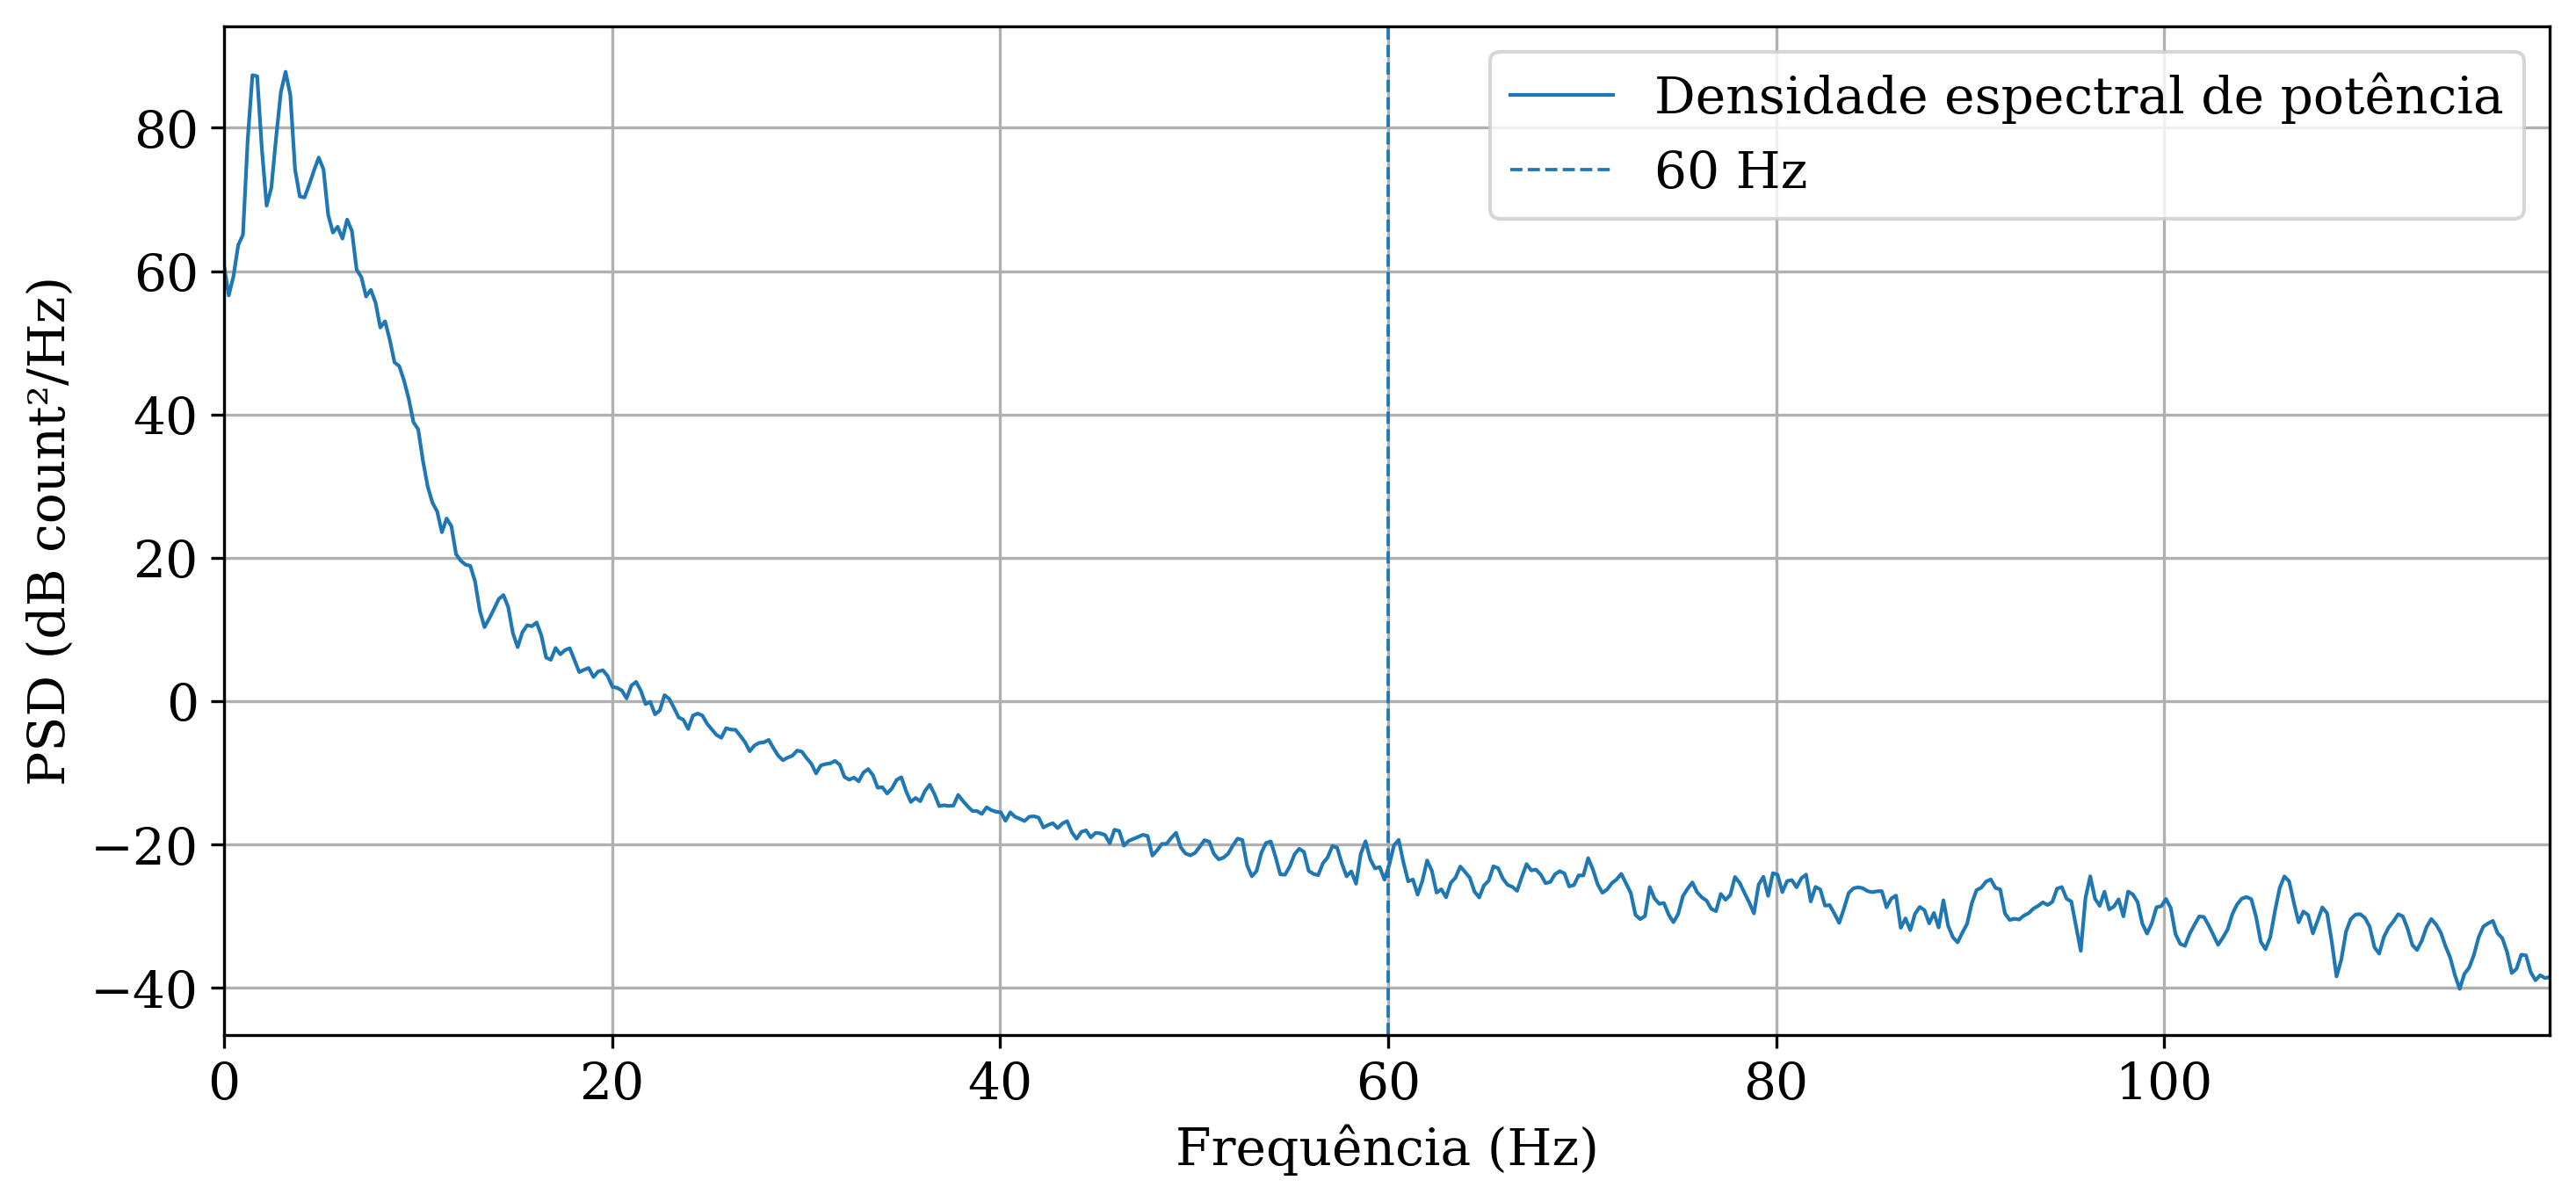
\includegraphics[width=\textwidth]{figuras/figura_ppg_espectro.png}
    \caption[Densidade espectral de potência do sinal de PPG]
    {Densidade espectral de potência do sinal de fotopletismografia (PPG) no intervalo de 0 a 120~Hz, expressa em $\mathrm{dB\,count^2/Hz}$. A linha tracejada vertical indica a frequência de 60~Hz, utilizada como referência para a avaliação de interferência proveniente da rede elétrica. Observa-se predominância do conteúdo espectral nas baixas frequências e redução acentuada da potência com o aumento da frequência.}
    \label{fig:ppg_espectro}
\end{figure}

A componente estimada em 60~Hz apresentou nível de $-78,85$~dB em relação ao valor eficaz do sinal filtrado. Não foi identificado um pico predominante nessa frequência, indicando baixa contribuição relativa da interferência da rede elétrica no sinal processado.

\subsubsection{Discussão do canal de PPG}
\label{subsubsec:discussao_ppg}

O canal apresentou variações periódicas, máximos pulsáteis repetitivos e frequência de pulso compatível com aquela obtida pelos canais de ECG. A elevada correlação entre os pulsos e o template indicou que a morfologia geral foi preservada durante o registro.

A amplitude apresentou maior variação que os intervalos temporais, comportamento esperado em sensores ópticos sujeitos a alterações de contato e movimento. Como não foram utilizados sensores independentes de pressão, iluminação ou movimento, não foi possível identificar isoladamente a origem de cada variação observada.

Os resultados demonstraram funcionamento compatível com a aquisição de PPG para fins de visualização e processamento funcional. Entretanto, não foram avaliados parâmetros como saturação periférica de oxigênio, perfusão absoluta ou indicadores clínicos derivados da forma de onda.

\subsection{Coerência funcional entre ECG e PPG}
\label{subsec:coerencia_ecg_ppg}

As frequências médias obtidas pelo ECG~1 e pelo PPG foram iguais dentro da precisão numérica da análise, correspondendo a aproximadamente 95,145~bpm. A diferença entre o ECG~2 e o PPG foi de apenas 0,0033~bpm, equivalente a aproximadamente 0,0034\%.

Foram associados 47 pares de eventos entre o ECG~1 e o PPG. O atraso aparente mediano entre o pico R e o máximo pulsátil subsequente foi de 200,006~ms, com média de 200,430~ms e desvio padrão de 1,156~ms. Para o ECG~2, o atraso aparente mediano foi de aproximadamente 201,004~ms.

A Figura~\ref{fig:coerencia_ecg_ppg} apresenta os sinais normalizados e os eventos correspondentes. Cada máximo pulsátil ocorreu depois do pico R associado, mantendo uma separação temporal aproximadamente constante ao longo do trecho analisado.

\begin{figure}[!htbp]
    \centering
    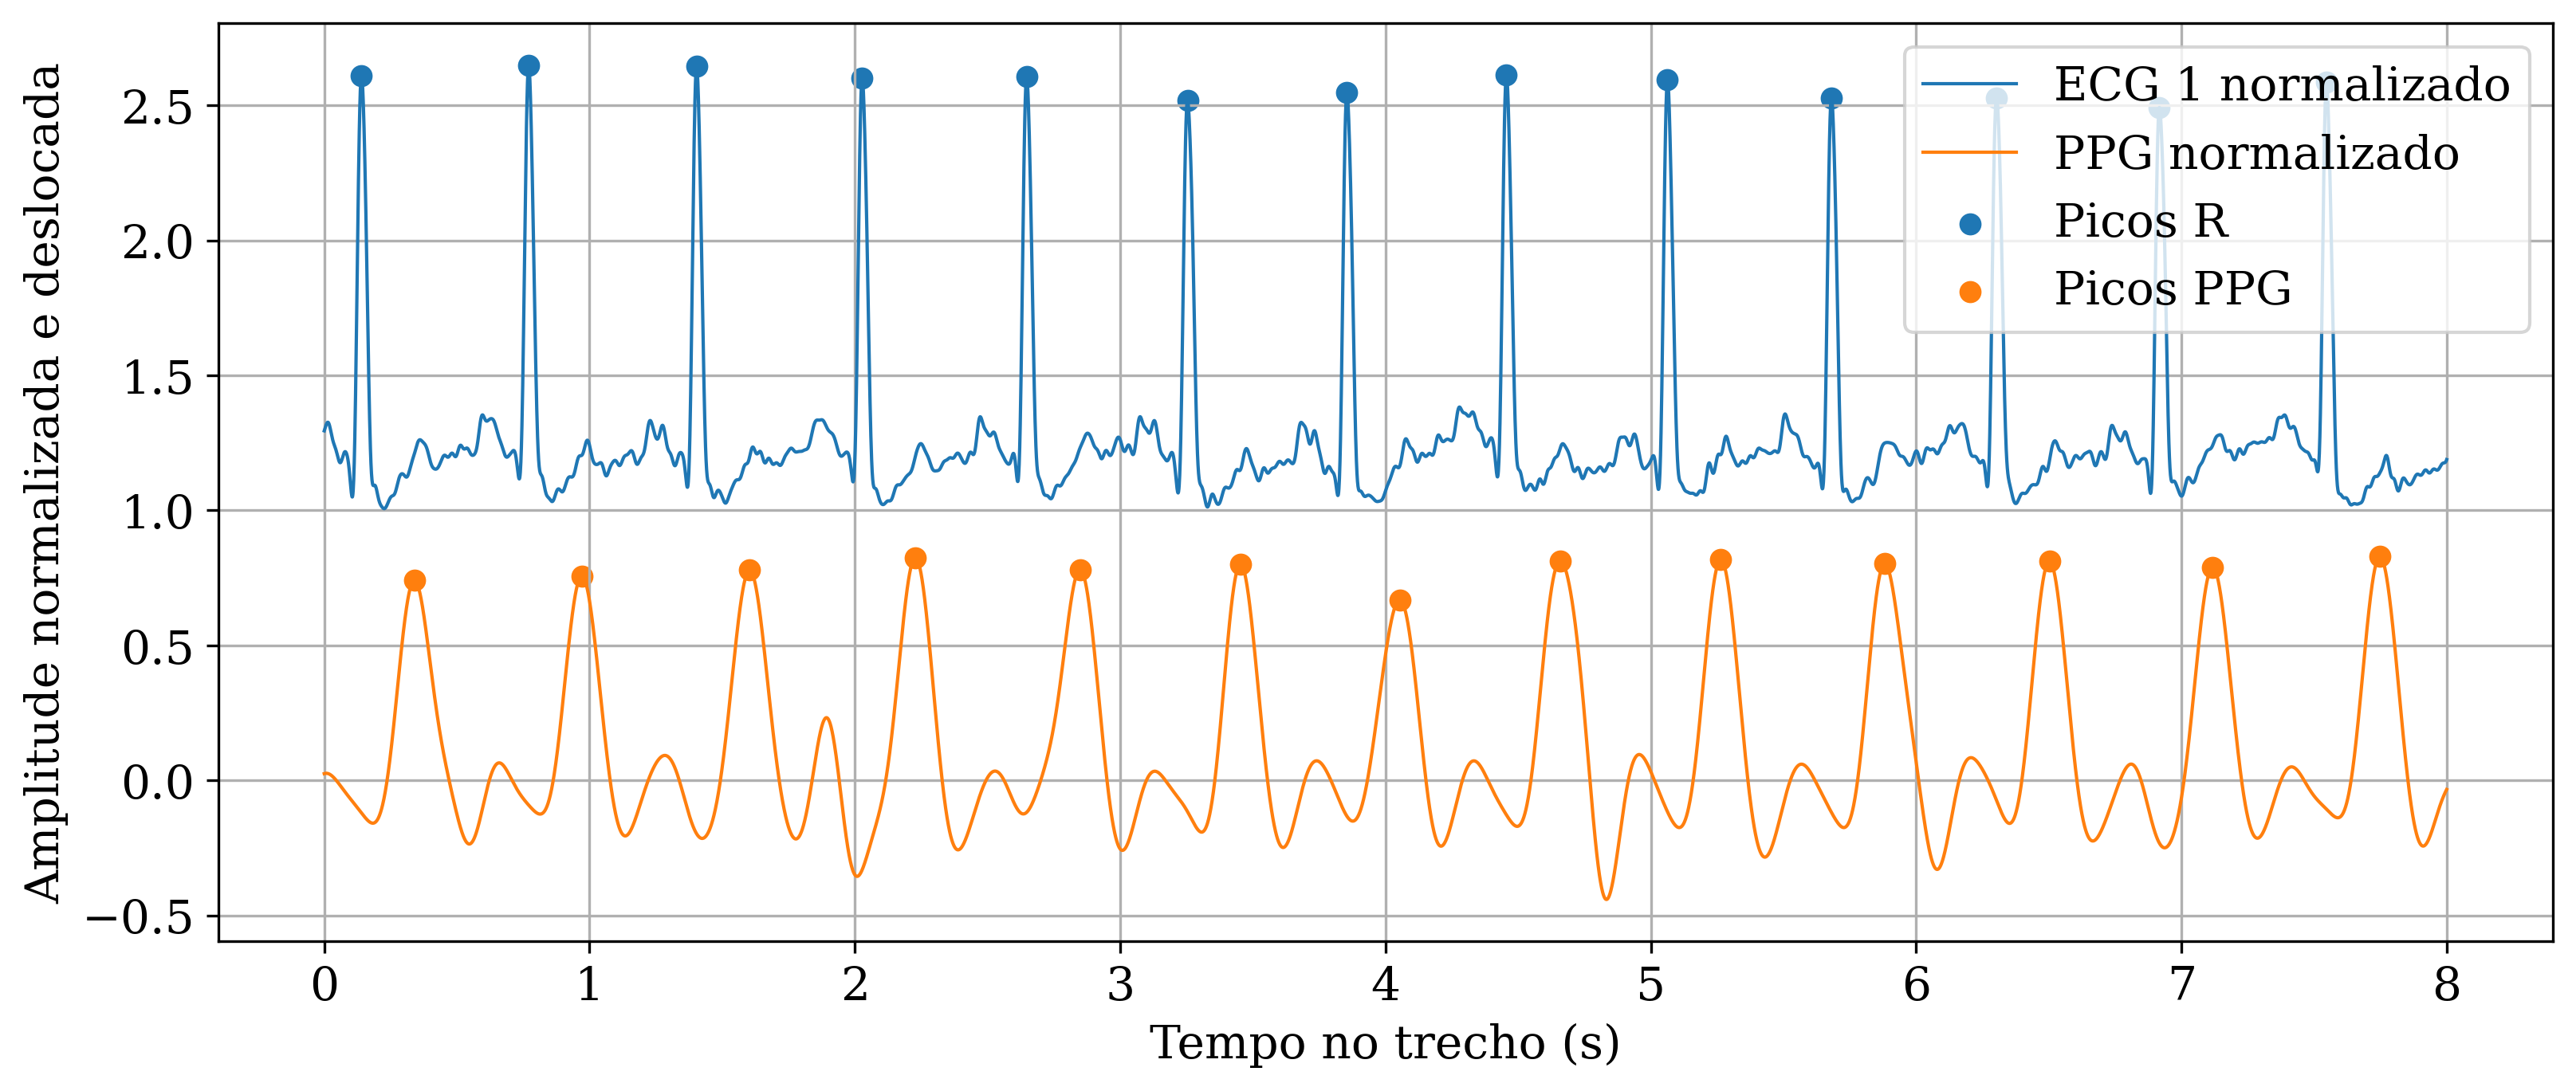
\includegraphics[width=\textwidth]{figuras/figura_coerencia_ecg_ppg.png}
    \caption[Correspondência temporal entre os picos do ECG e do PPG]
    {Comparação temporal, em um trecho representativo de 8~s, entre o primeiro canal de ECG e o sinal de fotopletismografia (PPG). Os sinais foram normalizados e deslocados verticalmente para evitar sobreposição. Os marcadores indicam os picos R detectados no ECG e os máximos pulsáteis identificados no PPG. Observa-se que cada pico do PPG ocorre após o pico R correspondente, evidenciando o atraso entre a atividade elétrica cardíaca e a chegada da onda de pulso ao local de medição periférica.}
    \label{fig:coerencia_ecg_ppg}
\end{figure}

A correspondência dos eventos e a proximidade entre as frequências forneceram evidência funcional de que os dois tipos de sinal refletiram o mesmo ritmo fisiológico durante o registro. O atraso observado foi compatível com a ocorrência do pulso periférico após a atividade elétrica cardíaca.

Esse atraso não foi interpretado como uma medida clínica de tempo de trânsito de pulso. A plataforma utiliza aquisição multiplexada, não foi sincronizada com um instrumento clínico e não passou por calibração específica para esse tipo de medição. Portanto, o valor foi utilizado apenas como indicador de coerência temporal entre os canais.

\subsection{Síntese funcional dos sinais fisiológicos}
\label{subsec:sintese_fisiologicos}

A Tabela~\ref{tab:sintese_fisiologicos} reúne os principais resultados funcionais dos três canais analisados.

\begin{table}[!htb]
    \centering
    \caption{Síntese funcional dos sinais fisiológicos adquiridos.}
    \label{tab:sintese_fisiologicos}
    \renewcommand{\arraystretch}{1.25}
    \begin{tabularx}{\textwidth}{
        >{\raggedright\arraybackslash}p{3.6cm}
        *{3}{>{\raggedright\arraybackslash}X}
    }
        \toprule
        \textbf{Parâmetro} &
        \multicolumn{1}{c}{\textbf{ECG 1}} &
        \multicolumn{1}{c}{\textbf{ECG 2}} &
        \multicolumn{1}{c}{\textbf{PPG}} \\
        \midrule

        \textbf{Tipo de sinal}
        & \multicolumn{1}{c}{ECG}
        & \multicolumn{1}{c}{ECG}
        & \multicolumn{1}{c}{PPG} \\

        \textbf{Eventos identificados}
        & \multicolumn{1}{c}{47}
        & \multicolumn{1}{c}{47}
        & \multicolumn{1}{c}{47} \\

        \textbf{Frequência média (bpm)}
        & \multicolumn{1}{c}{95,145}
        & \multicolumn{1}{c}{95,148}
        & \multicolumn{1}{c}{95,145} \\

        \textbf{Correlação mediana}
        & \multicolumn{1}{c}{0,9947}
        & \multicolumn{1}{c}{0,7859}
        & \multicolumn{1}{c}{0,9772} \\

        \textbf{Características identificadas}
        & Complexos QRS repetitivos, polaridade positiva e template com candidatos às ondas P e T.
        & Complexos QRS coincidentes com os do ECG~1, polaridade positiva e candidato posterior compatível com a onda T.
        & Componente pulsátil periódica, máximos regulares e template repetitivo. \\

        \textbf{Interferências e limitações}
        & Deriva da linha de base; amplitudes referentes à saída condicionada; componente de 60~Hz em $-82,89$~dB.
        & Menor amplitude e repetibilidade morfológica; 17,78\% dos batimentos com baixa correlação; componente de 60~Hz em $-64,13$~dB.
        & Variação de 12,59\% da amplitude pulsátil; possíveis efeitos de contato, movimento e iluminação, não separáveis a partir do registro. \\

        \bottomrule
    \end{tabularx}
\end{table}


A aquisição fisiológica apresentou taxa média próxima de 1~kS/s por canal, duração de aproximadamente 30~s e ausência de lacunas temporais. Os três canais foram identificados, armazenados e analisados na mesma base temporal, permitindo detectar 47 eventos correspondentes em cada sinal.

Os dois canais de ECG apresentaram complexos temporalmente coincidentes e estimativas praticamente idênticas da frequência cardíaca. O primeiro canal apresentou melhor repetibilidade e relação sinal-ruído, enquanto o segundo manteve a capacidade de detecção dos eventos apesar da menor amplitude e da maior irregularidade morfológica.

O canal de PPG apresentou frequência de pulso equivalente à frequência cardíaca estimada pelos canais de ECG e atraso aparente aproximadamente constante em relação aos picos R. Esses resultados demonstraram coerência funcional entre a atividade elétrica registrada pelos módulos de ECG e a variação pulsátil detectada pelo sensor óptico.

De forma geral, a plataforma foi capaz de adquirir, identificar, visualizar, armazenar e processar simultaneamente dois sinais de ECG e um sinal de PPG. Os registros apresentaram características compatíveis com os fenômenos fisiológicos esperados e foram suficientes para demonstrar o funcionamento multicanal da arquitetura, sem que isso constitua validação clínica, diagnóstica ou metrológica dos módulos utilizados.

% ============================================================================
\section{Discussão geral dos resultados}
\label{sec:discussao_geral}

Os resultados apresentados ao longo deste capítulo permitiram avaliar a plataforma em três níveis complementares. O primeiro correspondeu ao funcionamento integrado do hardware, do firmware e do software, incluindo a aquisição, a transmissão, a visualização e o armazenamento dos dados. O segundo compreendeu a verificação experimental da cadeia de aquisição por meio de sinais conhecidos, avaliados nos domínios do tempo e da frequência. O terceiro consistiu na aplicação funcional da arquitetura à aquisição simultânea de dois canais de ECG e um canal de PPG.

A análise conjunta mostrou que a plataforma foi capaz de adquirir sinais de diferentes formas, frequências e amplitudes, preservar sua identificação por canal e disponibilizar os dados brutos para processamento posterior. Ao mesmo tempo, os ensaios evidenciaram limitações relacionadas à continuidade de algumas sessões, à aquisição sequencial dos canais, à proximidade de determinadas componentes com o limite de Nyquist.

\subsection{Fidelidade dos sinais conhecidos}
\label{subsec:discussao_fidelidade}

Os ensaios com sinais conhecidos demonstraram elevada correspondência entre as frequências configuradas no gerador e as frequências estimadas a partir dos dados adquiridos. Considerando as senoides de 100 e 450~Hz, as ondas quadradas de 5 e 50~Hz e as frequências de repetição dos sinais multitom e sinc, os erros relativos permaneceram inferiores a 0,004\%. Esse resultado indica que, durante os segmentos regulares de aquisição, a base temporal utilizada pelo sistema foi suficiente para localizar corretamente as componentes fundamentais em toda a faixa experimental analisada.

As amplitudes medidas também permaneceram próximas dos valores configurados no gerador. Conforme o critério utilizado para cada forma de onda, os desvios ficaram aproximadamente entre 0,67\% e 2,94\%. Nas senoides, foi utilizada a amplitude pico a pico do sinal ou da componente fundamental ajustada, enquanto nas ondas quadradas a diferença entre os patamares representou melhor o comportamento regular da forma de onda. Nos sinais multitom e sinc, foi considerada a amplitude pico a pico observada no registro.

As comparações com o osciloscópio apresentaram diferenças geralmente limitadas a poucos pontos percentuais. Parte dessas diferenças decorreu dos critérios empregados pelos dois sistemas. O osciloscópio calculou algumas grandezas a partir dos valores extremos ou de algoritmos automáticos internos, enquanto o processamento dos dados adquiridos utilizou ajustes matemáticos, estimativas de patamares e análise dos registros completos. Assim, diferenças entre amplitude pico a pico, valor eficaz e amplitude da componente fundamental não indicam necessariamente uma alteração equivalente da forma de onda.

A senoide de 100~Hz apresentou elevada correspondência temporal com o modelo ajustado e aproximadamente dez amostras por período, permitindo reconhecer diretamente sua forma no registro. A senoide de 450~Hz também teve sua frequência fundamental corretamente identificada, mas foi representada por apenas aproximadamente 2,22 amostras por período. Nessa condição, a ligação visual entre pontos sucessivos não permite reconstruir com segurança a forma contínua do sinal, embora o ajuste e a análise espectral tenham demonstrado sua compatibilidade com uma componente próxima de 450~Hz.

A proximidade da senoide de 450~Hz com a frequência de Nyquist também afetou a interpretação das componentes harmônicas. Enquanto a fundamental permaneceu abaixo do limite e foi identificada corretamente, componentes de maior frequência puderam ultrapassar a primeira zona de Nyquist e reaparecer em frequências inferiores por rebatimento espectral. Esse comportamento reforça que o atendimento ao critério mínimo de Nyquist não garante, isoladamente, margem suficiente para a análise detalhada da morfologia ou da distorção harmônica.

As ondas quadradas evidenciaram de forma mais direta a influência da largura de banda disponível. A onda de 5~Hz apresentou patamares estáveis, ciclo de trabalho próximo de 50\% e primeiras harmônicas ímpares praticamente coincidentes com a distribuição teórica. Como sua frequência fundamental era reduzida em relação à taxa de aquisição, diversas componentes permaneceram abaixo do limite de Nyquist e contribuíram para a representação das transições.

Na onda quadrada de 50~Hz, a frequência, os patamares e o ciclo de trabalho também foram preservados, mas as harmônicas de maior ordem apresentaram atenuação progressiva. A terceira harmônica permaneceu próxima do comportamento teórico, enquanto os desvios aumentaram na quinta, na sétima e na nona harmônicas. Essa redução foi compatível com a aproximação das componentes ao limite superior da banda e com a resposta conjunta do gerador, da entrada analógica, do ADS1256 e do processo de amostragem.

Os tempos de subida e descida estimados para as ondas quadradas ficaram próximos ou abaixo de um intervalo de amostragem. Por essa razão, os valores obtidos por interpolação não representaram uma caracterização precisa das bordas analógicas. O sistema preservou a alternância entre os patamares, mas a taxa de 1~kS/s por canal não forneceu amostras intermediárias suficientes para comparar diretamente a forma das transições com as medições do osciloscópio.

O ensaio multitom demonstrou a capacidade da plataforma de separar componentes simultâneas. Os cinco tons entre 50 e 250~Hz foram identificados individualmente, com erros reduzidos de frequência e diferença máxima de amplitude relativa próxima de 0,07~dB. A preservação das amplitudes relativas indicou comportamento aproximadamente uniforme da cadeia de aquisição nessa faixa.

O sinal sinc permitiu avaliar uma forma com estrutura temporal e espectral mais ampla. O pulso principal, os cruzamentos por zero e os lóbulos laterais permaneceram reconhecíveis, enquanto o espectro apresentou linhas discretas distribuídas sob um envelope de grande largura. As diferenças em relação ao osciloscópio permaneceram limitadas a poucos pontos percentuais nas métricas temporais consideradas, embora a largura do pulso e a posição dos cruzamentos dependessem de interpolação entre amostras.

De forma geral, os ensaios mostraram que a plataforma preservou satisfatoriamente as frequências fundamentais, as amplitudes e as principais características temporais e espectrais dos sinais avaliados. As limitações tornaram-se mais evidentes nas transições rápidas e nas componentes próximas ao limite de Nyquist, condições em que uma taxa de aquisição superior e uma filtragem anti-aliasing mais restritiva ofereceriam maior margem para a análise.

\subsection{Desempenho da arquitetura multicanal}
\label{subsec:discussao_arquitetura_multicanal}

Durante os intervalos classificados como regulares, a taxa efetiva permaneceu próxima de 1~kS/s por canal. Nos três ensaios de bancada considerados na análise temporal, as taxas médias regulares ficaram entre aproximadamente 1000,14 e 1000,16~Hz, com erro inferior a 0,017\% em relação ao valor nominal. Os percentis superiores dos intervalos também permaneceram próximos de 1~ms, indicando baixa dispersão durante o funcionamento normal.

A principal limitação temporal observada nos ensaios de bancada não esteve na taxa dos intervalos regulares, mas na ocorrência ocasional de lacunas mais longas. Os percentuais estimados de perda foram de aproximadamente 3,05\% no ensaio com as senoides, 7,37\% no ensaio com as ondas quadradas e 3,52\% no ensaio com os sinais complexos. Essas interrupções reduziram a taxa global calculada sobre toda a duração das sessões, embora tenham permanecido disponíveis segmentos contíguos suficientes para as análises realizadas.

A sessão fisiológica apresentou comportamento distinto, com taxa média de aproximadamente 999,98~Hz, ausência de lacunas temporais e armazenamento de toda a aquisição em um único segmento contíguo. Esse resultado mostrou que a plataforma foi capaz de manter uma sessão multicanal de aproximadamente 30~s sem perdas detectáveis, mas a variação observada entre os diferentes registros indica que a continuidade ainda depende das condições de execução e deve ser aperfeiçoada antes de se afirmar desempenho ininterrupto em períodos prolongados.

Os quadros armazenados mantiveram ordem crescente, identificação fixa dos canais e marcações temporais monotônicas. Não foram observados saltos nos identificadores sequenciais nem troca das posições associadas às entradas. Essa organização permitiu comparar sinais adquiridos no mesmo ciclo de varredura e realizar o processamento posterior sem necessidade de reconstruir a associação entre os canais.

A utilização de um único ADS1256 implicou aquisição multiplexada. Os pares diferenciais foram selecionados sequencialmente, de modo que as amostras presentes em um mesmo quadro não foram convertidas exatamente no mesmo instante. A marcação temporal associada ao quadro representa o ciclo de aquisição, mas não elimina a pequena defasagem interna entre os canais. Essa característica não comprometeu as análises realizadas, porém deve ser considerada em aplicações que exijam sincronização temporal mais rigorosa.

Foram observadas componentes espectrais de um sinal em frequências relacionadas ao outro canal adquirido simultaneamente. Entretanto, algumas dessas componentes também coincidiram com harmônicas, aliases ou interferências externas. Por esse motivo, os resultados não permitem quantificar isoladamente a diafonia da plataforma. Uma avaliação específica exigiria excitar apenas uma entrada e manter as demais em condições elétricas controladas.

A separação entre a rotina de visualização e a rotina de armazenamento foi importante para o funcionamento da arquitetura. O software limitou a quantidade de pontos exibidos e a frequência de atualização gráfica sem reduzir o conjunto de dados gravado. Dessa forma, a interface pôde operar no Raspberry Pi 3 B+ ao mesmo tempo em que os valores brutos, as marcações temporais e os metadados eram preservados nos arquivos HDF5.

O armazenamento incremental e a possibilidade de recuperação e exportação das sessões também contribuíram para a reutilização dos dados. Os registros puderam ser processados posteriormente sem depender das operações realizadas durante a visualização, preservando a distinção entre sinal bruto e produtos derivados de filtragem ou análise.

\subsection{Adequação da plataforma para aquisição de ECG e PPG}
\label{subsec:discussao_ecg_ppg}

A aquisição fisiológica demonstrou que a arquitetura foi capaz de registrar simultaneamente dois sinais de ECG e um sinal de PPG, mantendo sua identificação e uma base temporal comum. Foram detectados 47 eventos correspondentes em cada canal, com frequências médias próximas de 95,15~bpm. A coincidência dos eventos nos dois canais de ECG e a equivalência entre a frequência cardíaca e a frequência de pulso forneceram evidência funcional de que os registros representaram o mesmo ritmo fisiológico.

O primeiro canal de ECG apresentou complexos QRS de elevada amplitude e alta repetibilidade morfológica. A correlação mediana entre os batimentos e o template foi superior a 0,99, e estruturas anteriores e posteriores ao QRS puderam ser reconhecidas no template médio. Esses elementos foram compatíveis com a organização esperada para um sinal eletrocardiográfico, embora não tenham sido utilizados para medir intervalos clínicos.

O segundo canal apresentou complexos temporalmente coincidentes com aqueles do primeiro, mas sua amplitude foi significativamente menor e a participação de ruído foi superior. A correlação mediana dos batimentos com o template foi aproximadamente 0,79, e parte dos eventos apresentou menor semelhança morfológica. Ainda assim, todos os picos R foram associados aos eventos do primeiro canal e produziram praticamente a mesma estimativa de frequência cardíaca.

A diferença entre os canais demonstrou a influência do posicionamento dos eletrodos, da orientação da derivação, das características dos módulos de condicionamento e das conexões utilizadas. Como as amplitudes foram medidas após a etapa de condicionamento, seus valores não representam diretamente os potenciais presentes na superfície corporal e não permitem comparação fisiológica absoluta entre os canais.

O sinal de PPG apresentou máximos pulsáteis regulares, template repetitivo e frequência de pulso equivalente àquela obtida pelos canais de ECG. A amplitude pulsátil apresentou maior variação que os intervalos temporais, comportamento compatível com a sensibilidade dos sensores ópticos a alterações de contato, pressão, movimento e iluminação.

As componentes de 60~Hz permaneceram abaixo do conteúdo principal dos sinais processados. O segundo canal de ECG apresentou maior participação relativa dessa frequência que o primeiro canal e o PPG, mas ela não constituiu a componente dominante em nenhum dos registros. A filtragem digital contribuiu para reduzir interferências e deriva de linha de base, mantendo os dados brutos disponíveis para reprocessamento.

O atraso aparente entre os picos R e os máximos do PPG permaneceu próximo de 200~ms e apresentou baixa dispersão no trecho analisado. Esse resultado reforçou a coerência temporal entre a atividade elétrica cardíaca e a resposta pulsátil periférica. Entretanto, o valor não foi interpretado como medida clínica de tempo de trânsito de pulso, pois a arquitetura utiliza aquisição multiplexada e não foi calibrada ou comparada com um sistema clínico para essa finalidade.

Os resultados fisiológicos demonstraram adequação funcional inicial da plataforma para ECG e PPG. Essa conclusão se restringe à capacidade de adquirir, visualizar, armazenar e processar sinais com características compatíveis com os fenômenos esperados. Não foram avaliados desempenho diagnóstico, segurança para uso assistencial, exatidão de parâmetros clínicos ou conformidade regulatória de um equipamento médico.


\subsection{Limitações experimentais}
\label{subsec:limitacoes_experimentais}

A primeira limitação decorreu da utilização de um único conversor multiplexado. Os canais foram lidos sequencialmente e não de forma estritamente simultânea. Embora os dados tenham sido organizados no mesmo quadro, existe uma defasagem entre as conversões individuais, que não foi medida separadamente para cada entrada.

A marcação temporal foi associada ao quadro multicanal e não individualmente a cada conversão. Essa organização foi suficiente para os ensaios realizados, mas limita aplicações que dependam de sincronização precisa entre eventos muito rápidos em canais diferentes.

As lacunas temporais observadas em algumas sessões de bancada constituíram outra limitação. A causa específica das interrupções não foi isolada experimentalmente e pode envolver a transmissão USB bloqueante, o fluxo de armazenamento, a concorrência com outras operações ou a interação entre as diferentes camadas do sistema. Embora os segmentos contíguos tenham permitido realizar as análises previstas, a ocorrência dessas lacunas limita o uso do protótipo em aplicações que exijam registro ininterrupto de eventos transitórios.

Cada configuração de bancada foi avaliada a partir de uma sessão principal de aproximadamente 30~s. Não foram realizadas repetições suficientes para caracterizar estatisticamente a variabilidade entre montagens, inicializações ou dias de ensaio. Dessa forma, os resultados descrevem o comportamento observado nas sessões analisadas e não representam intervalos de confiança para o desempenho geral da plataforma.

O osciloscópio foi utilizado como referência visual e paramétrica, principalmente por meio de capturas e medições automáticas. Não foram empregados registros numéricos integralmente sincronizados entre o osciloscópio e a plataforma para todas as formas de onda. Por esse motivo, a comparação foi baseada em grandezas como frequência, amplitude, valor eficaz, ciclo de trabalho e largura do pulso, e não em uma comparação ponto a ponto de todos os sinais.

A senoide de 450~Hz e as harmônicas superiores da onda quadrada de 50~Hz ficaram próximas do limite de Nyquist. Nessa região, a representação temporal possui poucos pontos por período e as componentes acima de 500~Hz estão sujeitas a aliasing. Essa condição limita a análise das harmônicas e impede inferir a forma analógica completa somente a partir dos dados adquiridos.

Os tempos de subida e descida das ondas quadradas também não puderam ser determinados com precisão, pois ocorreram em uma escala próxima ao período de amostragem. As estimativas interpoladas descrevem a transição entre amostras, mas não substituem a medição realizada por um instrumento com largura de banda e taxa de amostragem superiores.

A aquisição fisiológica foi direcionada à demonstração funcional e não incluiu comparação simultânea com eletrocardiógrafo, oxímetro ou outro equipamento clínico certificado. Também não foram adotados protocolos destinados a avaliar diferentes sujeitos, posições anatômicas, condições de movimento ou variações ambientais. Consequentemente, os resultados não permitem atribuir exatidão clínica às frequências, amplitudes, intervalos ou morfologias obtidas.

Os artefatos presentes nos sinais fisiológicos não puderam ser associados isoladamente a movimento, pressão de contato, iluminação, posicionamento dos eletrodos ou características dos módulos. A ausência de sensores auxiliares de movimento, pressão ou luminosidade impediu separar quantitativamente essas contribuições.

A presença de componentes coincidentes com o sinal aplicado ao outro canal não permitiu determinar diretamente a diafonia, pois algumas frequências também correspondiam a harmônicas, aliases ou interferência da rede. Uma caracterização específica exigiria entradas terminadas de forma controlada e excitação individual de cada canal.

A expansão para outros sinais fisiológicos foi prevista na arquitetura, mas não foi demonstrada experimentalmente além do ECG e do PPG. O quarto canal incluiu uma informação auxiliar de temperatura no arquivo analisado, mas esse dado não foi submetido a uma avaliação funcional equivalente àquela realizada para os demais sinais.

Por fim, as dimensões, a massa, a autonomia da bateria e o custo médio de reposição ainda devem ser consolidados para permitir uma avaliação quantitativa completa da portabilidade e do baixo custo. A montagem em placa perfurada foi adequada ao protótipo acadêmico, mas uma versão destinada a uso fora de bancada exigiria placa de circuito impresso, estrutura mecânica, conectores protegidos e avaliação adicional de segurança elétrica.


\chapter{Conclusão}
\label{cap:conclusao}

Este trabalho apresentou o desenvolvimento e a verificação experimental de uma plataforma portátil e modular destinada à aquisição, à visualização, ao processamento e ao armazenamento de múltiplos sinais fisiológicos. A proposta partiu da necessidade de uma solução experimental aberta, capaz de integrar módulos de condicionamento distintos em uma cadeia comum de digitalização e processamento, mantendo acesso aos dados brutos, identificação dos canais e possibilidade de expansão do hardware e do software.

A arquitetura desenvolvida integrou módulos independentes de condicionamento, o conversor analógico-digital ADS1256, uma placa STM32 Black Pill e uma Raspberry Pi 3 Model B+. A STM32 foi responsável pelo controle do conversor, pelo chaveamento sequencial dos quatro pares diferenciais, pela organização das amostras em quadros e pela transmissão dos dados por USB CDC. Na Raspberry Pi, o software realizou a recepção, a validação e a separação dos dados por canal, além de disponibilizar visualização nos domínios do tempo e da frequência, aplicação de filtros digitais e armazenamento incremental das sessões em arquivos HDF5.

A separação entre aquisição, visualização, processamento e armazenamento constituiu um dos principais resultados da implementação. Os valores brutos foram preservados independentemente das operações aplicadas na interface, permitindo que os sinais fossem posteriormente reabertos, exportados e submetidos a novas rotinas de análise. Dessa forma, o sistema não ficou limitado às métricas ou aos filtros disponíveis durante a aquisição, possibilitando auditoria, reprocessamento e desenvolvimento incremental de novas formas de análise.

A verificação da cadeia de aquisição com sinais conhecidos demonstrou que a plataforma foi capaz de preservar as principais características temporais e espectrais das formas de onda avaliadas. Nos ensaios com senoides de 100~Hz e 450~Hz, ondas quadradas de 5~Hz e 50~Hz, sinal multitom e sinal sinc, os erros relativos de frequência permaneceram inferiores a 0,004\%. As amplitudes adquiridas também permaneceram próximas aos valores configurados no gerador e às medidas obtidas pelo osciloscópio, considerando as diferenças entre os critérios de cálculo empregados pelos dois sistemas.

Os ensaios também evidenciaram os limites impostos pela taxa de 1~kS/s por canal. A senoide de 100~Hz apresentou aproximadamente dez amostras por período e elevada correspondência com o modelo ajustado. Para a senoide de 450~Hz, a frequência fundamental foi identificada corretamente, mas a disponibilidade de aproximadamente 2,22 amostras por período restringiu a representação direta da forma de onda e reduziu a margem em relação ao limite de Nyquist.

Nas ondas quadradas, os patamares, os períodos e os ciclos de trabalho foram preservados. A onda de 5~Hz apresentou componentes harmônicas próximas da distribuição teórica de uma onda quadrada ideal, enquanto a onda de 50~Hz mostrou atenuação crescente das harmônicas de maior ordem. Os tempos de subida e descida não puderam ser caracterizados com precisão, pois as transições ocorreram em uma escala próxima ao intervalo de amostragem.

O sinal multitom demonstrou que a plataforma foi capaz de identificar e separar cinco componentes simultâneas distribuídas entre 50 e 250~Hz, mantendo pequena variação relativa de amplitude entre os tons. O sinal sinc permitiu verificar a aquisição de uma forma de onda com pulso principal, cruzamentos por zero, lóbulos laterais e conteúdo espectral amplo. Esses resultados mostraram que a cadeia não se restringiu à aquisição de sinais periódicos simples, mantendo capacidade de representar sinais com estruturas temporais e espectrais compostas.

A análise do desempenho temporal mostrou que, nos intervalos regulares, a taxa efetiva permaneceu próxima de 1~kS/s por canal, com erros inferiores a 0,017\% nas sessões de bancada consideradas. A principal limitação não esteve na frequência do ciclo regular de aquisição, mas na ocorrência ocasional de lacunas temporais. Os registros de bancada apresentaram percentuais estimados de perdas entre aproximadamente 3,05\% e 7,37\%, embora tenham mantido segmentos contíguos suficientes para as análises realizadas.

A aquisição fisiológica apresentou comportamento mais estável. Durante aproximadamente 30~s, foram armazenados 29.750 quadros com taxa média próxima de 1~kS/s, sem lacunas temporais, saltos de sequência ou marcações não monotônicas. Os dois canais de ECG e o canal de PPG foram mantidos em uma mesma base temporal e identificados corretamente durante toda a sessão.

Nos sinais fisiológicos, foram detectados 47 eventos correspondentes nos dois canais de ECG e no PPG, com frequência média próxima de 95,15~bpm. O primeiro canal de ECG apresentou complexos QRS bem definidos e elevada repetibilidade morfológica. O segundo canal apresentou menor amplitude e maior participação de ruído, mas manteve coincidência temporal dos eventos e estimativa de frequência cardíaca equivalente à do primeiro canal.

O canal de PPG apresentou variações pulsáteis regulares, morfologia repetitiva e frequência de pulso compatível com a frequência cardíaca estimada pelos sinais de ECG. O atraso aparente entre os picos R e os máximos pulsáteis permaneceu próximo de 200~ms, fornecendo evidência funcional de que os sinais estavam associados ao mesmo ciclo cardiovascular. Esse valor não foi interpretado como medida clínica, uma vez que a plataforma não foi calibrada para determinar tempo de trânsito de pulso e utiliza aquisição multiplexada.

Os resultados fisiológicos demonstraram a capacidade funcional da arquitetura de adquirir simultaneamente sinais de naturezas elétrica e óptica, preservar sua identificação, armazená-los e permitir análises temporais, espectrais e morfológicas. Essa demonstração não constitui validação clínica ou diagnóstica. As amplitudes analisadas correspondem às saídas dos módulos de condicionamento na entrada do conversor, e não diretamente aos potenciais fisiológicos originais.

Em relação aos objetivos específicos, foram implementadas a arquitetura de hardware, a configuração e o controle do conversor, a aquisição multicanal, a transmissão estruturada, o software de recepção, a visualização durante a coleta, o armazenamento dos dados brutos e as rotinas básicas de filtragem e análise. A cadeia foi verificada experimentalmente com sinais conhecidos e aplicada à aquisição de ECG e PPG.

A escalabilidade foi demonstrada pela divisão da plataforma em módulos funcionais, pela disponibilidade de quatro pares diferenciais e pela organização configurável dos canais no firmware e no software. A portabilidade foi demonstrada funcionalmente pelo uso da Raspberry Pi, da tela integrada e da alimentação por bateria. A utilização de componentes comerciais e de ferramentas de software amplamente disponíveis sustenta a proposta de uma solução de custo reduzido em comparação com sistemas laboratoriais dedicados.

O objetivo geral pode, portanto, ser considerado substancialmente atendido. Foi entregue uma plataforma funcional capaz de adquirir, identificar, visualizar, processar e armazenar múltiplos sinais, mantendo acesso aos dados brutos e interfaces que permitem sua expansão. A ressalva principal refere-se ao requisito de aquisição contínua, uma vez que, apesar da ausência de perdas na sessão fisiológica, as lacunas observadas em parte dos ensaios de bancada mostram que a continuidade ainda não foi garantida em todas as condições de operação.

A contribuição concreta do trabalho consiste na disponibilização de uma base experimental integrada e reutilizável para aquisição multicanal de sinais fisiológicos. Antes do desenvolvimento, os diferentes módulos de sensores, a conversão analógico-digital, o controle, a visualização e o armazenamento constituíam elementos separados. Após sua integração, tornou-se possível conectar módulos de condicionamento distintos a um núcleo comum, acompanhar os sinais durante a coleta, preservar os registros brutos e realizar novas análises sem depender de um equipamento dedicado a um único tipo de sinal.

A plataforma desenvolvida não substitui equipamentos médicos certificados e não se destina à tomada de decisão clínica. Seu uso atual está voltado à pesquisa, ao ensino, à prototipagem e à avaliação experimental de sistemas de aquisição. Eventual evolução para uma aplicação assistencial exigiria verificação de segurança elétrica, desempenho metrológico, biocompatibilidade dos elementos de contato, proteção dos dados, confiabilidade de longo prazo e atendimento aos requisitos regulatórios aplicáveis.

\section{Possibilidades de aperfeiçoamento}
\label{sec:possibilidades_aperfeicoamento}

O aperfeiçoamento prioritário consiste na redução das lacunas temporais observadas nos ensaios de bancada. Entre as modificações tecnicamente viáveis estão a implementação de buffers adicionais no firmware, o envio não bloqueante por USB, o agrupamento de múltiplos quadros em uma única transferência e a revisão da concorrência entre recepção, gravação e atualização da interface. Essas alterações devem ser acompanhadas por ensaios prolongados que permitam verificar a continuidade durante períodos superiores aos utilizados neste trabalho.

A sincronização entre os canais pode ser aprimorada pela inclusão de uma marcação temporal associada a cada conversão ou pela adoção de conversores capazes de amostragem simultânea. Essa modificação seria especialmente relevante para análises que dependam de diferenças temporais pequenas entre canais, como propagação de pulsos, relações de fase ou comparação de eventos rápidos.

A cadeia analógica pode ser aperfeiçoada com filtros anti-aliasing definidos para cada tipo de sinal e com possibilidade de configurar taxas de aquisição diferentes conforme o conteúdo espectral dos canais. Para sinais com componentes próximas a 500~Hz ou com transições rápidas, uma taxa superior a 1~kS/s proporcionaria maior margem para representação temporal e análise harmônica.

A montagem em placa perfurada pode ser substituída por uma placa de circuito impresso dedicada, com conectores protegidos, distribuição de alimentação revisada, planos de referência e blindagem apropriada. Uma estrutura mecânica integrada também permitiria caracterizar de forma mais completa as dimensões, a massa, a resistência física e a autonomia do sistema.

A caracterização experimental pode ser ampliada por meio de repetições das sessões, ensaios de longa duração, avaliação controlada da diafonia, medições com entradas terminadas e comparação numérica sincronizada com instrumentos de referência. Nos sinais fisiológicos, futuras avaliações podem incluir diferentes posicionamentos de eletrodos, condições de movimento, sensores de referência e comparação simultânea com equipamentos clínicos, mantendo-se a distinção entre verificação técnica e validação para uso assistencial.

A arquitetura permite ainda a integração de módulos destinados a outros sinais, como temperatura, atividade eletrodérmica, eletromiografia e respiração. A inclusão desses módulos deverá considerar suas faixas de amplitude, conteúdo espectral, necessidades de condicionamento, segurança elétrica e impacto sobre a taxa de aquisição dos canais já implementados.

Com esses aperfeiçoamentos, a plataforma poderá evoluir de um protótipo acadêmico funcional para uma infraestrutura experimental mais robusta, capaz de apoiar estudos envolvendo aquisição prolongada, integração de novos sensores e desenvolvimento de métodos de processamento de sinais fisiológicos, preservando o caráter aberto e modular estabelecido neste trabalho.

% ==============================================================================
% Referências
% ==============================================================================
\bibliography{referencias}

\end{document}
